% Arquivo LaTeX de exemplo de dissertação/tese a ser apresentada à CPG do IME-USP
%
% Criação: Jesús P. Mena-Chalco
% Revisão: Fabio Kon e Paulo Feofiloff
% Adaptação para UTF8, biblatex e outras melhorias: Nelson Lago
%
% Except where otherwise indicated, these files are distributed under
% the MIT Licence. The example text, which includes the tutorial and
% examples as well as the explanatory comments in the source, are
% available under the Creative Commons Attribution International
% Licence, v4.0 (CC-BY 4.0) - https://creativecommons.org/licenses/by/4.0/


%%%%%%%%%%%%%%%%%%%%%%%%%%%%%%%%%%%%%%%%%%%%%%%%%%%%%%%%%%%%%%%%%%%%%%%%%%%%%%%%
%%%%%%%%%%%%%%%%%%%%%%%%%%%%%%% PREÂMBULO LaTeX %%%%%%%%%%%%%%%%%%%%%%%%%%%%%%%%
%%%%%%%%%%%%%%%%%%%%%%%%%%%%%%%%%%%%%%%%%%%%%%%%%%%%%%%%%%%%%%%%%%%%%%%%%%%%%%%%

% A opção twoside (frente-e-verso) significa que a aparência das páginas pares
% e ímpares pode ser diferente. Por exemplo, as margens podem ser diferentes ou
% os números de página podem aparecer à direita ou à esquerda alternadamente.
% Mas nada impede que você crie um documento "só frente" e, ao imprimir, faça
% a impressão frente-e-verso.
%
% Aqui também definimos a língua padrão do documento
% (a última da lista) e línguas adicionais.
\documentclass[12pt,twoside,brazilian,english]{book}
% \documentclass[12pt,twoside,english,brazilian]{book}

% Ao invés de definir o tamanho das margens, vamos definir os tamanhos do
% texto, do cabeçalho e do rodapé, e deixamos a package geometry calcular
% o tamanho das margens em função do tamanho do papel. Assim, obtemos o
% mesmo resultado impresso, mas com margens diferentes, se o tamanho do
% papel for diferente.
\usepackage[a4paper]{geometry}

\geometry{
  textwidth=152mm,
  hmarginratio=12:17, % 24:34 -> com papel A4, 24mm + 152mm + 34mm = 210mm
  textheight=237mm,
  vmarginratio=8:7, % 32:28 -> com papel A4, 32mm + 237mm + 28mm = 297mm
  headsep=11mm, % distância entre a base do cabeçalho e o texto
  headheight=21mm, % qualquer medida grande o suficiente, p.ex., top - headsep
  footskip=10mm,
  marginpar=20mm,
  marginparsep=5mm,
}

% Vários pacotes e opções de configuração genéricos; para personalizar o
% resultado, modifique estes arquivos.
%%%%%%%%%%%%%%%%%%%%%%%%%%%%%%%%%%%%%%%%%%%%%%%%%%%%%%%%%%%%%%%%%%%%%%%%%%%%%%%%
%%%%%%%%%%%%%%%%%%%%%%% CONFIGURAÇÕES E PACOTES BÁSICOS %%%%%%%%%%%%%%%%%%%%%%%%
%%%%%%%%%%%%%%%%%%%%%%%%%%%%%%%%%%%%%%%%%%%%%%%%%%%%%%%%%%%%%%%%%%%%%%%%%%%%%%%%

% Vários comandos auxiliares para o desenvolvimento de packages e classes;
% aqui, usamos em alguns comandos de formatação e condicionais.
\usepackage{etoolbox}
%\RequirePackage{pdftexcmds}
\usepackage{letltxmacro}
%\usepackage{ltxcmds}

% LaTeX 3
\usepackage{expl3}
\usepackage{xparse}

%\usepackage{filehook}

% Detecta se estamos usando pdftex, luatex, xetex etc.
\usepackage{iftex}

%\usepackage{xfp} % Floating-point calculations

\usepackage{regexpatch}

% O projeto LaTeX3 renomeou algumas macros em 2019-03-05 e removeu
% a compatibilidade com os nomes antigos em 2020-07-17 a partir de
% 2021-01-01 (veja o arquivo l3deprecation.dtx e o changelog em
% https://github.com/latex3/latex3/blob/main/l3kernel/CHANGELOG.md).
% Isso afetou a package regexpatch: versões antigas da package não
% funcionam com versões novas de LaTeX e vice-versa. Infelizmente,
% ubuntu 21.04 (hirsute) e debian 11 (bullseye) incluem essas versões
% incompatíveis e, portanto, a package regexpatch não funciona nesses
% ambientes. Talvez fosse possível contornar esse problema com a
% package latexrelease, mas isso afetaria muitos outros recursos.
% Ao invés disso, vamos restaurar manualmente a compatibilidade.
% TODO: remover isto após debian bullseye se tornar obsoleta,
%       provavelmente no final de 2024.
\makeatletter
\ExplSyntaxOn
\@ifpackagelater{regexpatch}{2021/03/21}
  {} % Se regexpatch é "nova", expl3 deve ser também; nada a fazer
  {
    % Talvez o correto seja 2021/01/01, mas na prática o resultado é o mesmo
    \@ifpackagelater{expl3}{2020/07/17}
      {
        % As versões são incompatíveis; vamos recuperar as macros preteridas
        \cs_gset:Npn \token_get_prefix_spec:N { \cs_prefix_spec:N }
        \cs_gset:Npn \token_get_arg_spec:N { \cs_argument_spec:N }
        \cs_gset:Npn \token_get_replacement_spec:N { \cs_replacement_spec:N }
      }
      {} % As duas packages são antigas e, portanto, compatíveis entre si
  }
\ExplSyntaxOff
\makeatother

% Algumas packages dependem de xpatch e tentam carregá-la, causando conflitos
% com regexpatch. Como regexpatch oferece todos os recursos de xpatch (ela
% é uma versão estendida de xpatch, mas ainda considerada experimental), vamos
% fazê-las acreditar que xpatch já foi carregada.
\makeatletter
\@ifpackagelater{regexpatch}{2020/10/06}
    {\expandafter\xdef\csname ver@xpatch.sty\endcsname{2020/03/25}}
    {\expandafter\xdef\csname ver@xpatch.sty\endcsname{2012/10/02}}
\makeatother

% Acrescenta a correção deste bug (contida na release 2018-11-28):
% https://github.com/latex3/latex2e/issues/94 . Se a correção não
% puder ser aplicada, temos uma versão de LaTeX que já a incorpora.
% Esse bug afeta apenas textos em duas colunas.
% TODO: remover após ubuntu 18.04 se tornar obsoleta (abril/2023)
\makeatletter
\patchcmd\@combinedblfloats{\box\@outputbox}{\unvbox\@outputbox}{}{}
\makeatother

% Arithmetic expressions in \set{length,counter} & \addto{length,counter};
% commands \widthof, \heightof, \depthof, \totalheightof, \settototalheight
\usepackage{calc}

% Algumas packages "padrão" da AMS, que são praticamente obrigatórias.
% Algumas delas devem ser carregadas antes de unicode-math ou das
% definições das fontes do documento. É preciso carregar amsthm após
% amsmath para o comando \qedhere funcionar dentro do ambiente align.
\usepackage{amssymb}
\usepackage{amsmath}
\usepackage{amsthm}

% "fontenc" é um parâmetro do NFSS (sistema de gestão de fontes do
% LaTeX; consulte "texdoc fntguide" e "texdoc fontenc"). O default
% é OT1, mas ele tem algumas limitações; a mais importante é que,
% com ele, palavras acentuadas não podem ser hifenizadas. Por
% conta disso, quase todos os documentos LaTeX utilizam o fontenc
% T1. A escolha do fontenc tem consequências para as fontes que
% podem ser usadas com NFSS; hoje em dia T1 tem mais opções de
% qualidade, então não se perde nada em usá-lo. A package fontspec
% (para gestão de fontes usando outro mecanismo, compatível apenas
% com lualatex e xelatex) carrega fontenc automaticamente, mas
% usando outra codificação ("TU" e não "T1"). Ainda assim, é útil
% carregar o fontenc T1 (antes de carregar fontspec!) para o caso
% de alguma fonte "antiga" ser utilizada no documento (embora isso
% não seja recomendado: lualatex e xelatex só são capazes de
% hifenizar palavras acentuadas com o fontenc TU).
\usepackage[T1]{fontenc}

\ifPDFTeX
  % O texto está escrito em utf8.
  \usepackage[utf8]{inputenc}

  % Várias packages que definem as fontes do documento carregam fontaxes,
  % mas carregamos aqui porque, com qualquer fonte, ela permite utilizar
  % small caps + itálico. Algumas raras packages de fontes podem causar
  % conflitos com fontaxes, em geral por utilizarem a package "concorrente"
  % nfssext-cfr.
  %
  % TODO A funcionalidade pela qual faz sentido carregar fontaxes aqui
  %      (small caps + itálico) foi incorporada ao kernel do LaTeX na
  %      versão 2020-02-02, então está em TeXLive 2021. Remover isto
  %      quando arxiv usar TeXLive >= 2021 e ubuntu 20.04 (focal) for
  %      descontinuada (abril de 2025). As packages que precisam de
  %      fontaxes podem continuar a carregá-la sem problemas.
  \usepackage{fontaxes}

  % LaTeX substitui algumas sequências de caracteres, como
  % "fi", "fl" e outras, por caracteres especiais ("ligaduras").
  % Para que seja possível fazer copiar/colar ou buscas por
  % textos contendo essas ligaduras, o arquivo PDF precisa
  % conter uma tabela indicando quais são elas. Com fontes
  % OTF (LuaLaTeX ou XeLaTeX) isso não costuma ser um problema,
  % mas com pdfLaTeX pode ser. Estes dois comandos (que só
  % existem no pdfLaTeX) incluem uma tabela genérica que
  % funciona para a maioria das fontes. Veja a seção 5 de
  % http://www.tug.org/TUGboat/Articles/tb29-1/tb91thanh-fonts.pdf
  % Note que alguns visualizadores de PDF tentam "adivinhar"
  % o conteúdo da tabela quando ela está incompleta ou não
  % existe, então copiar/colar e buscas podem funcionar em
  % alguns visualizadores e em outros não.
  %
  % TODO Isto foi incluído no kernel do LaTeX versão 2021-06-01,
  %      então está em TeXLive 2022. Remover isto quando arxiv
  %      usar TeXLive >= 2022 e ubuntu 22.04 (jammy) for
  %      descontinuada (abril de 2027).
  \input glyphtounicode.tex
  \pdfgentounicode=1
\else
  % Não é preciso carregar inputenc com LuaTeX e XeTeX, pois
  % com eles utf8 é obrigatório.
  \usepackage{fontspec}

  % Ao invés de usar o sistema tradicional de LaTeX para gerir
  % as fontes matemáticas, utiliza as extensões matemáticas do
  % formato otf definidas pela microsoft. Ao ativar esta package
  % o mecanismo tradicional não funciona mais! Há poucas fontes
  % com suporte a unicode-math.
  \usepackage{unicode-math}
\fi

% Acesso a símbolos adicionais, como \textrightarrow, \texteuro etc.,
% disponíveis na maioria das fontes através do fontenc TS1 ou mudando
% momentaneamente para computer modern/latin modern. Raramente útil
% com lualatex/xelatex, mas não causa problemas. Várias packages de
% fontes carregam textcomp, às vezes com opções específicas; assim,
% para evitar problemas, vamos carregá-la no final do preâmbulo para
% o caso de ela não ter sido carregada antes.
%
% TODO A funcionalidade oferecida por textcomp foi incorporada ao kernel
%      do LaTeX na versão 2020-02-02, então está em TeXLive 2021. Remover
%      isto quando arxiv usar TeXLive >= 2021 e ubuntu 20.04 (focal) for
%      descontinuada (abril de 2025). As packages que precisam de textcomp
%      podem continuar a carregá-la sem problemas.
\AtBeginDocument{\usepackage{textcomp}}

% TeXLive 2018 inclui a versão 2.7a da package microtype e a versão
% 1.07 de luatex. Essa combinação faz aparecer um bug:
% https://tex.stackexchange.com/a/476742
% Aqui, aplicamos a solução sugerida, que não tem "contra-indicações".
% TODO: remover após ubuntu 18.04 se tornar obsoleta (abril/2023)
\ifLuaTeX
  \usepackage{luatexbase}
\fi

% microajustes no tamanho das letras, espaçamento etc. para melhorar
% a qualidade visual do resultado.
\usepackage{microtype}

% Alguns "truques" (sujos?) para minimizar over/underfull boxes.
%
% Para fazer um texto justificado, é preciso modificar o tamanho dos espaços
% em cada linha para mais ou para menos em relação ao seu tamanho ideal. Para
% escolher as quebras de linha, TeX vai percorrendo o texto procurando lugares
% possíveis para quebrar as linhas considerando essa flexibilidade mas dentro
% de um certo limite mínimo/máximo. Nesse processo, ele associa a cada possível
% linha o valor *badness*, que é o nível de distorção do tamanho dos espaços
% daquela linha em relação ao ideal, e ignora opções que tenham badness muito
% grande (esse limite é dado por \tolerance). Depois de encontradas todas
% as possíveis quebras de linha e a badness de cada uma, TeX calcula as
% *penalties* das quebras encontradas, que são uma medida de quebras "ruins".
% Por exemplo, na configuração padrão, quebrar uma linha hifenizando uma
% palavra gera uma penalty de 50; já uma quebra que faça a última linha
% do parágrafo ficar sozinha na página seguinte gera uma penalty de 150.
% Finalmente, TeX calcula a "feiúra" de cada possível linha (demerits)
% com base na badness e nas penalties e escolhe a solução que minimiza os
% demerits totais do parágrafo. Os comandos \linebreak e \pagebreak funcionam
% simplesmente acrescentando uma penalty negativa ao lugar desejado para a
% quebra.
%
% Para cada fonte, o espaço entre palavras tem um tamanho ideal, um
% tamanho mínimo e um tamanho máximo (é possível obter os valores com
% \number\fontdimenX\font\relax, veja https://tex.stackexchange.com/q/88991 ).
% TeX nunca reduz um espaço para menos que o mínimo da fonte, mas pode
% aumentá-lo para mais que o máximo. Se os espaços de uma linha ficam
% com o tamanho ideal, a badness da linha é 0; se o tamanho é
% reduzido/aumentado 50% do mínimo/máximo, a badness da linha é 12; se
% o tamanho é reduzido/aumentado para o mínimo/máximo, a badness é 100,
% e assim por diante. O valor máximo possível para badness é 10.000, que
% significa "badness infinita". Como é feito o cálculo: se as medidas
% do espaço definidas pela fonte são "x plus y minus z" e o tamanho
% final do espaço é "x + k*y" ou "x - k*z", a badness é 100*(k^3). Com
% Libertinus corpo 12, os valores são "3pt plus 1.5pt minus .9996pt",
% Então se o espaço tiver sido aumentado para 3.75pt, o fator é 0.5 e
% a badness é 100*(.5^3) = 12.
%
% \tolerance indica a badness máxima que TeX aceita para uma linha; seu valor
% default é 200. Assim, aumentar para, digamos, 300 ou 400, permite que
% TeX escolha parágrafos com maior variação no espaçamento entre as palavras.
% No entanto, no cálculo de demerits, a badness e as penalties de cada linha
% são elevadas ao quadrado, então TeX geralmente prefere escolher outras
% opções no lugar de uma linha com espaçamento ruim. Por exemplo, órfãs/viúvas
% têm demerit de 22.500 e dois hífens seguidos têm demerit de 10.000; já uma
% linha com badness 400 tem demerit 160.000. Portanto, não é surpreendente que
% a maioria dos parágrafos tenha demerits abaixo de 40.000, quase todos abaixo
% de 100.000 e praticamente nenhum acima de 1.000.000. Isso significa que, para
% a grande maioria dos parágrafos, aumentar \tolerance não faz diferença: uma
% linha com badness 400 nunca será efetivamente escolhida se houver qualquer
% outra opção com badness menor. Também fica claro que não há muita diferença
% real entre definir \tolerance como 800 ou 9.999 (a não ser fazer TeX
% trabalhar mais desnecessariamente).
%
% O problema muda de figura se TeX não consegue encontrar uma solução. Isso
% pode acontecer em dois casos: (1) o parágrafo tem ao menos uma linha que não
% pode ser quebrada com badness < 10.000 ou (2) o parágrafo tem ao menos uma
% linha que não pode ser quebrada com badness < tolerance (mas essa badness é
% menor que 10.000).
%
% No primeiro caso, se houver várias possibilidades de linhas que não podem ser
% quebradas, TeX não vai ser capaz de compará-las e escolher a melhor: todas
% têm a badness máxima (10.000) e, portanto, a que gerar menos deméritos no
% restante do parágrafo será a escolhida. Na realidade, no entanto, essas
% linhas *não* são igualmente ruins entre si, o que pode levar TeX a fazer uma
% má escolha. Para evitar isso, TeX tenta novamente aplicando
% \emergencystretch, que "faz de conta" que o tamanho máximo ideal dos espaços
% da linha é maior que o definido na fonte. Isso reduz a badness de todas as
% linhas, o que soa parecido com aumentar \tolerance. Há três diferenças, no
% entanto: (1) essa mudança só afeta os parágrafos que falharam; (2) soluções
% que originalmente teriam badness = 10.000 (e, portanto, seriam vistas como
% equivalentes) podem ser avaliadas e comparadas entre si; e (3) como a badness
% de todas as linhas diminui, a possibilidade de outras linhas que
% originalmente tinham badness alta serem escolhidas aumenta. Esse último ponto
% significa que \emergencystretch pode fazer TeX escolher linhas mais
% espaçadas, fazendo o espaçamento do parágrafo inteiro aumentar e, portanto,
% tornando o resultado mais homogêneo mesmo com uma linha particularmente ruim.
%
% É esse último ponto que justifica o uso de \emergencystretch no segundo caso
% também: apenas aumentar a tolerância, nesse caso, poderia levar TeX a
% diagramar uma linha ruim em meio a um parágrafo bom, enquanto
% \emergencystretch pode fazer TeX aumentar o espaçamento de maneira geral no
% parágrafo, minimizando o contraste da linha problemática com as demais.
% Colocando a questão de outra maneira, aumentar \tolerance para lidar com
% esses parágrafos problemáticos pode fazê-los ter uma linha especialmente
% ruim, enquanto \emergencystretch pode dividir o erro entre várias linhas.
% Assim, definir \tolerance em torno de 800 parece razoável: no caso geral,
% não há diferença e, se um desses casos difíceis não pode ser resolvido com
% uma linha de badness até 800, \emergencystretch deve ser capaz de gerar um
% resultado igual ou melhor.
%
% Penalties & demerits: https://tex.stackexchange.com/a/51264
% Definições (fussy, sloppy etc.): https://tex.stackexchange.com/a/241355
% Mais definições (hfuzz, hbadness etc.): https://tex.stackexchange.com/a/50850
% Donald Arseneau defendendo o uso de \sloppy: https://groups.google.com/d/msg/comp.text.tex/Dhf0xxuQ66E/QTZ7aLYrdQUJ
% Artigo detalhado sobre \emergencystretch: https://www.tug.org/TUGboat/tb38-1/tb118wermuth.pdf
% Esse artigo me leva a crer que algo em torno de 1.5em é suficiente

\tolerance=800
\hyphenpenalty=100 % Default 50; se o texto é em 2 colunas, 50 é melhor
\setlength{\emergencystretch}{1.5em}

% Não gera warnings para Overfull menor que 1pt
\hfuzz=1pt
\vfuzz\hfuzz

% Não gera warnings para Underfull com badness < 1000
\hbadness=1000
\vbadness=1000

% Por padrão, o algoritmo LaTeX para textos não-justificados é (muito) ruim;
% este pacote implementa um algoritmo bem melhor
\usepackage[newcommands]{ragged2e}

% ragged2e funciona porque permite que LaTeX hifenize palavras em textos
% não-justificados quando necessário. No caso de textos centralizados,
% no entanto, isso em geral não é desejável. Assim, newcommands não é
% interessante para \centering e \begin{center}. newcommands também
% causa problemas com legendas se o float correspondente usa \centering
% (o que é muito comum). Assim, vamos voltar \centering e \begin{center}
% à definição padrão.
\let\centering\LaTeXcentering
\let\center\LaTeXcenter
\let\endcenter\endLaTeXcenter

% Com ragged2e e a opção "newcommands", textos curtos não-justificados
% podem gerar warnings sobre "underfull \hbox". Não há razão para pensar
% muito nesses warnings, então melhor desabilitá-los.
% https://tex.stackexchange.com/a/18019
\makeatletter
\gappto{\raggedright}{\hbadness=\@M}
\gappto{\RaggedRight}{\hbadness=\@M}
\gappto{\raggedleft}{\hbadness=\@M}
\gappto{\RaggedLeft}{\hbadness=\@M}
\gappto{\Centering}{\hbadness=\@M} % not \centering
\gappto{\flushleft}{\hbadness=\@M}
\gappto{\FlushLeft}{\hbadness=\@M}
\gappto{\flushright}{\hbadness=\@M}
\gappto{\FlushRight}{\hbadness=\@M}
\gappto{\Center}{\hbadness=\@M} % not \center
\makeatother

% Espaçamento entre linhas configurável (\singlespacing, \onehalfspacing etc.)
\usepackage{setspace}

% LaTeX às vezes coloca notas de rodapé logo após o final do texto da
% página ao invés de no final da página; este pacote evita isso e faz
% notas de rodapé funcionarem corretamente em títulos de seções.
% Esta package deve ser carregada depois de setspace.
\usepackage[stable,bottom]{footmisc}

% Se uma página está vazia, não imprime número de página ou cabeçalho
\usepackage{emptypage}

% hyperref deve preferencialmente ser carregada próximo ao final
% do preâmbulo mas, para o caso de alguma package forçar a sua
% carga antes de executarmos \usepackage explicitamente, vamos
% garantir que estas opções estejam ativas.
\PassOptionsToPackage{
  unicode=true,
  pdfencoding=unicode,
  plainpages=false,
  pdfpagelabels,
  bookmarksopen=true,
  breaklinks=true,
  %hyperfootnotes=false, % polui desnecessariamente com bordercolor
}{hyperref}

% Carrega nomes de cores disponíveis (podem ser usados com hyperref e listings)
\usepackage[hyperref,svgnames,x11names,table]{xcolor}

% LaTeX oferece 2 pares de comandos nativos para mudar textos para caixa
% alta ou baixa: \uppercase ou \lowercase (TeX "puro") e \MakeUppercase
% ou \MakeLowecase (LaTeX), mas esses comandos têm algumas limitações
% (https://tug.org/TUGboat/tb41-1/tb127wright-case.pdf ). Esta package
% define os comandos \MakeTextUppercase e \MakeTextLowercase que resolvem
% isso.
% TODO: quando TeXLive 2023 for a versão mais antiga de LaTeX a que
%       estivermos dando suporte, podemos eliminar a package textcase
%       e usar \MakeUppercase e \MakeLowercase diretamente. A partir
%       dessa versão, essas macros usam \text_[upper|lower]case:n de
%       expl3.
\usepackage{textcase}

% Em documentos frente-e-verso, LaTeX faz o final da página terminar sempre
% no mesmo lugar (exceto no final dos capítulos). Esse comportamento pode ser
% ativado explicitamente com o comando "\flushbottom". Mas se, por alguma
% razão, o volume de texto na página é "pequeno", essa página vai ter espaços
% verticais artificialmente grandes. Uma solução para esse problema é utilizar
% "\raggedbottom" (padrão em documentos que não são frente-e-verso): com essa
% opção, as páginas podem terminar em alturas ligeiramente diferentes. Outra
% opção é corrigir manualmente cada página problemática, por exemplo com o
% comando "\enlargethispage".
%\raggedbottom
\flushbottom

% Por padrão, LaTeX coloca uma espaço aumentado após sinais de pontuação;
% Isso não é tão bom quanto alguns TeX-eiros defendem :) .
% Esta opção desabilita isso e, consequentemente, evita problemas com
% "id est" (i.e.) e "exempli gratia" (e.g.)
\frenchspacing

% Mais recursos para trechos de texto "puro" (tabs, quebras de linha etc.
% não são modificados), além do ambiente "\begin{comment}".
\usepackage{verbatim}

% Durante o processamento, LaTeX procura por arquivos adicionais necessários
% (tanto componentes do próprio LaTeX, como packages e fontes, quanto partes
% do conteúdo em si, como imagens carregadas com \includegraphics ou arquivos
% solicitados com \input ou \include) no diretório de instalação e também
% no diretório atual (ou seja, o diretório do projeto). Assim, normalmente
% é preciso usar caminhos relativos para incluir arquivos de subdiretórios:
% "\input{diretorio/arquivo}". No entanto, há duas limitações:
%
% 1. É necessário dizer "\input{diretorio/arquivo}" mesmo quando o arquivo
%    que contém esse comando já está dentro do subdiretório.
%
% 2. Isso não deve ser usado para packages ("\usepackage{diretorio/package}"),
%    embora na prática funcione.
%
% Há três maneiras recomendadas de resolver esses problemas:
%
% 1. Acrescentando os diretórios desejados ao arquivo texmf.cnf
%
% 2. Acrescentando os diretórios desejados às variáveis de ambiente
%    TEXINPUTS e BSTINPUTS
%
% 3. Colocando os arquivos adicionais na árvore TEXMF (geralmente, no
%    diretório texmf dentro do diretório do usuário).
%
% Essas soluções, no entanto, não podem ser automatizadas por este modelo
% e são um tanto complicadas para usuários menos experientes. Veja mais a
% respeito na seção 5 de "texdoc kpathsea" e em
% https://www.overleaf.com/learn/latex/Articles/An_introduction_to_Kpathsea_and_how_TeX_engines_search_for_files .
%
% A package import pode solucionar o primeiro problema, mas exige o uso
% de outro comando no lugar de \input, então não a usamos aqui.
%\usepackage{import}
%
% Uma solução mais simples é acrescentar os diretórios desejados à macro
% \input@path, originalmente criada para resolver um problema relacionado
% à portabilidade. Seu uso não é normalmente recomendado por razões de
% desempenho, mas no nosso caso (em que adicionamos apenas um diretório
% com poucos arquivos e com máquinas modernas) isso não é um problema. Veja
% https://tex.stackexchange.com/questions/241828/define-path-for-packages-in-the-latex-file-analog-of-inputpath-or-graphicspa#comment705011_241832
\csappto{input@path}{{extras/}}

%%%%%%%%%%%%%%%%%%%%%%%%%%%%%%%%%%%%%%%%%%%%%%%%%%%%%%%%%%%%%%%%%%%%%%%%%%%%%%%%
%%%%%%%%%%%%%%%%%%%%%%%%%%%%%%%%%%% LÍNGUAS %%%%%%%%%%%%%%%%%%%%%%%%%%%%%%%%%%%%
%%%%%%%%%%%%%%%%%%%%%%%%%%%%%%%%%%%%%%%%%%%%%%%%%%%%%%%%%%%%%%%%%%%%%%%%%%%%%%%%

\makeatletter
\ExplSyntaxOn

% We need to have at least some variant of Portuguese and of English
% loaded to generate the abstract/resumo, palavras-chave/keywords etc.
% We will make sure that both languages are present in the class options
% list by adding them if needed. With this, these options become global
% and therefore are seen by all packages (among them, babel).
%
% babel traditionally uses "portuguese", "brazilian", "portuges", or
% "brazil" to support the Portuguese language, using .ldf files. babel
% is also in the process of implementing a new scheme, using .ini
% files, based on the concept of "locales" instead of "languages". This
% mechanism uses the names "portuguese-portugal", "portuguese-brazil",
% "portuguese-pt", "portuguese-br", "portuguese", "brazilian", "pt",
% "pt-PT", and "pt-BR" (i.e., neither "portuges" nor "brazil"). To avoid
% compatibility problems, let's stick with "brazilian" or "portuguese"
% by substituting portuges and brazil if necessary.

\NewDocumentCommand\@IMEportugueseAndEnglish{m}{

  % Make sure any instances of "portuges" and "brazil" are replaced
  % by "portuguese" e "brazilian"; other options are unchanged.
  \seq_gclear_new:N \l_tmpa_seq
  \seq_gclear_new:N \l_tmpb_seq
  \seq_gset_from_clist:Nc \l_tmpa_seq {#1}

  \seq_map_inline:Nn \l_tmpa_seq{
    \def\@tempa{##1}
    \ifstrequal{portuges}{##1}
      {
        \GenericInfo{sbc2019}{}{Substituting~language~portuges~->~portuguese}
        \def\@tempa{portuguese}
      }
      {}
    \ifstrequal{brazil}{##1}
      {
        \GenericInfo{}{Substituting~language~brazil~->~brazilian}
        \def\@tempa{brazilian}
      }
      {}
    \seq_gput_right:NV \l_tmpb_seq {\@tempa}
  }

  % Remove the leftmost duplicates (default is to remove the rightmost ones).
  % Necessary in case the user did "portuges,portuguese", "brazil,brazilian"
  % or some variation: When we substitute the language, we end up with the
  % exact same language twice, which may mess up the main language selection.
  \seq_greverse:N \l_tmpb_seq
  \seq_gremove_duplicates:N \l_tmpb_seq
  \seq_greverse:N \l_tmpb_seq

  % If the user failed to select some variation of English and Portuguese,
  % we add them here. We also remember which ones of portuguese/brazilian,
  % english/american/british etc. were selected.
  \exp_args:Nnx \regex_extract_all:nnNTF
    {\b(portuguese|brazilian)\b}
    {\seq_use:Nn \l_tmpb_seq {,}}
    \l_tmpa_tl
    {
      \tl_reverse:N \l_tmpa_tl
      \xdef\@IMEpt{\tl_head:N \l_tmpa_tl}
    }
    {
      \seq_gput_left:Nn \l_tmpb_seq {brazilian}
      \gdef\@IMEpt{brazilian}
    }

  \exp_args:Nnx \regex_extract_all:nnNTF
    {\b(english|american|USenglish|canadian|british|UKenglish|australian|newzealand)\b}
    {\seq_use:Nn \l_tmpb_seq {,}}
    \l_tmpa_tl
    {
      \tl_reverse:N \l_tmpa_tl
      \xdef\@IMEen{\tl_head:N \l_tmpa_tl}
    }
    {
      \seq_gput_left:Nn \l_tmpb_seq {english}
      \gdef\@IMEen{english}
    }

  \exp_args:Nc \xdef {#1} {\seq_use:Nn \l_tmpb_seq {,}}
}


% https://tex.stackexchange.com/a/43541
% This message is part of a larger thread that discusses some
% limitations of this method, but it is enough for us here.
\def\@getcl@ss#1.cls#2\relax{\def\@currentclass{#1}}
\def\@getclass{\expandafter\@getcl@ss\@filelist\relax}
\@getclass

% The three class option lists we need to update: \@unusedoptionlist,
% \@classoptionslist and one of \opt@book.cls, \opt@article.cls etc.
% according to the current class. Note that beamer.cls (and maybe
% others) does not use \@unusedoptionlist; with it, we incorrectly
% add "english,brazilian" to \@unusedoptionlist, but that does not
% cause problems.
\@IMEportugueseAndEnglish{@unusedoptionlist}
\@IMEportugueseAndEnglish{@classoptionslist}
\@IMEportugueseAndEnglish{opt@\@currentclass .cls}

\ExplSyntaxOff
\makeatother

% Babel permite definir a língua ou línguas usadas no documento e deve
% ser um dos primeiros pacotes a serem carregados. É possível definir
% as línguas como parâmetro aqui, mas já fizemos isso ao carregar a
% classe, no início do documento.
%
% A escolha da língua afeta quatro coisas:
%
% 1. A internacionalização das palavras criadas automaticamente, como
%    "Capítulo/Chapter", "Sumário/Table of Contents" etc. - babel chama
%    essas palavras de "captions";
%
% 2. A hifenização das palavras;
%
% 3. Algumas convenções tipográficas. Por exemplo, em francês é usual
%    acrescentar um espaço antes de caracteres como "?" e "!"; línguas
%    diferentes usam caracteres diferentes para as aspas tipográficas;
%    com algumas línguas asiáticas, pode ser necessário utilizar uma
%    fonte diferente etc.;
%
% 4. Atalhos (shorthands) - algumas línguas definem "atalhos" (shorthands"),
%    ou seja, tratam alguns caracteres como comandos especiais; por exemplo,
%    em francês o espaço que é colocado antes da exclamação funciona porque
%    o caracter "!" é, na verdade, um comando.
%
%%%% MUDANDO A LÍNGUA E HIFENIZAÇÃO %%%%
%
% Cada documento tem uma língua padrão; quando usamos pequenos trechos em
% outra língua, como por exemplo em citações, queremos alterar apenas os
% aspectos 2, 3 e 4; nesse caso, a troca da língua deve ser feita com
% \foreignlanguage{língua}{texto} ou com \begin{otherlanguage*}{língua}.
% Para alterar todos os quatro aspectos, deve-se usar \selectlanguage{língua}
% (que altera a língua padrão a partir desse ponto) ou
% \begin{otherlanguage}{língua}{texto}, que faz a alteração apenas até
% \end{otherlanguage}. Se você quiser apenas desabilitar a hifenização de
% um trecho de texto, pode usar \begin{hyphenrules}{nohyphenation}.
% Finalmente, com \babeltags é possível definir comandos curtos como
% "\textbr" (para "brazilian") que são equivalentes a \foreignlanguage.
%
%%%% PERSONALIZANDO CAPTIONS %%%%
%
% É possível personalizar os captions. Para versões de babel a partir
% de 3.51 (lançada em outubro de 2020), basta fazer
% \setlocalecaption{english}{contents}{Table of Contents}. Com versões
% anteriores, por razões históricas há dois mecanismos para fazer isso,
% então é preciso checar qual deve ser usado para cada língua (veja a
% documentação de babel ou faça um teste). São eles:
%
%   1. \renewcommand\spanishchaptername{Capítulo}
%
%   2. \addto\captionsenglish{\renewcommand\contentsname{Table of Contents}}
%      (este é o mais comum)
%
% Esses métodos valem também para a bibliografia, mas apenas se você
% estiver usando bibtex; com biblatex, que é o padrão neste modelo, é
% melhor usar o comando "\DefineBibliographyStrings" (veja a documentação
% de biblatex).
%
% Quando babel faz uma troca de língua, ele executa \extraslíngua e, se for
% necessário trocar os "captions", \captionslíngua (ou seja, os comandos
% acima modificam \captionslíngua). Então, se você quiser executar algo a
% mais quando uma língua é selecionada, faça \addto\extrasenglish{\blah}.
\usepackage{babel}
\usepackage{iflang}

% Por padrão, LaTeX utiliza maiúsculas no início de cada palavra nestas
% expressões ("Lista de Figuras"); vamos usar maiúsculas apenas na primeira
% palavra.
\addto\captionsbrazilian{%
  \renewcommand\listfigurename{Lista de figuras}%
  \renewcommand\listtablename{Lista de tabelas}%
  \renewcommand\indexname{Índice remissivo}%
}

% Alguns pacotes (tikz, siunitx) usam, além de babel, este pacote como
% auxiliar para a tradução de palavras-chave, como os meses do ano.
\usepackage{translator}

%%%%%%%%%%%%%%%%%%%%%%%%%%%%%%%%%%%%%%%%%%%%%%%%%%%%%%%%%%%%%%%%%%%%%%%%%%%%%%%%
%%%%%%%%%%%%%%%%%%%%%%%%%%%%%%%%%%% FONTE %%%%%%%%%%%%%%%%%%%%%%%%%%%%%%%%%%%%%%
%%%%%%%%%%%%%%%%%%%%%%%%%%%%%%%%%%%%%%%%%%%%%%%%%%%%%%%%%%%%%%%%%%%%%%%%%%%%%%%%

% LaTeX normalmente usa quatro tipos de fonte:
%
% * uma fonte serifada, para o corpo do texto;
% * uma fonte com design similar à anterior, para modo matemático;
% * uma fonte sem serifa, para títulos ou "entidades". Por exemplo, "a classe
%   \textsf{TimeManager} é responsável..." ou "chamamos \textsf{primos} os
%   números que...". Observe que em quase todos os casos desse tipo é mais
%   adequado usar negrito ou itálico;
% * uma fonte "teletype", para trechos de programas.
%
% A escolha de uma família de fontes para o documento normalmente é feita
% carregando uma package específica que, em geral, seleciona as quatro fontes
% de uma vez.
%
% LaTeX usa por default a família de fontes "Computer Modern". Essas fontes
% precisaram ser re-criadas diversas vezes em formatos diferentes, então há
% diversas variantes dela. Com o fontenc OT1 (default "ruim" do LaTeX), a
% versão usada é a BlueSky Computer Modern, que é de boa qualidade, mas com
% os problemas do OT1. Com fontenc T1 (padrão deste modelo e recomendado), o
% LaTeX usa o conjunto "cm-super". Com fontspec (ou seja, com LuaLaTeX e
% XeLaTeX), LaTeX utiliza a versão "Latin Modern". Ao longo do tempo, versões
% diferentes dessas fontes foram recomendadas como "a melhor"; atualmente, a
% melhor opção para usar a família Computer Modern é a versão "Latin Modern".
%
% Você normalmente não precisa lidar com isso, mas pode ser útil saber: O
% mecanismo tradicionalmente usado por LaTeX para gerir fontes é o NFSS
% (veja "texdoc fntguide"). Ele funciona com todas as versões de LaTeX,
% mas só com fontes que foram adaptadas para funcionar com LaTeX. LuaLaTeX
% e XeLaTeX podem usar NFSS mas também são capazes de utilizar um outro
% mecanismo (através da package fontspec), que permite utilizar quaisquer
% fontes instaladas no computador.

\ifPDFTeX
    % Usando pdfLaTeX

    % Ativa Latin Modern como a fonte padrão.
    \usepackage{lmodern}

    % Alguns truques para melhorar a aparência das fontes Latin Modern;
    % eles não funcionam com LuaLaTeX e XeLaTeX.

    % Latin Modern não tem fontes bold + Small Caps, mas cm-super sim;
    % assim, vamos ativar o suporte às fontes cm-super (sem ativá-las
    % como a fonte padrão do documento) e configurar substituições
    % automáticas para que a fonte Latin Modern seja substituída por
    % cm-super quando o texto for bold + Small Caps.
    \usepackage{fix-cm}

    % Com Latin Modern, é preciso incluir substituições para o encoding TS1
    % também por conta dos números oldstyle, porque para inclui-los nas fontes
    % computer modern foi feita uma hack: os dígitos são declarados como sendo
    % os números itálicos da fonte matemática e, portanto, estão no encoding TS1.
    %
    % Primeiro forçamos o LaTeX a carregar a fonte Latin Modern (ou seja, ler
    % o arquivo que inclui "DeclareFontFamily") e, a seguir, definimos a
    % substituição
    \fontencoding{TS1}\fontfamily{lmr}\selectfont
    \DeclareFontShape{TS1}{lmr}{b}{sc}{<->ssub * cmr/bx/n}{}
    \DeclareFontShape{TS1}{lmr}{bx}{sc}{<->ssub * cmr/bx/n}{}

    \fontencoding{T1}\fontfamily{lmr}\selectfont
    \DeclareFontShape{T1}{lmr}{b}{sc}{<->ssub * cmr/bx/sc}{}
    \DeclareFontShape{T1}{lmr}{bx}{sc}{<->ssub * cmr/bx/sc}{}

    % Latin Modern não tem "small caps + itálico", mas tem "small caps + slanted";
    % vamos definir mais uma substituição aqui.
    \fontencoding{T1}\fontfamily{lmr}\selectfont % já feito acima, mas tudo bem
    \DeclareFontShape{T1}{lmr}{m}{scit}{<->ssub * lmr/m/scsl}{}
    \DeclareFontShape{T1}{lmr}{bx}{scit}{<->ssub * lmr/bx/scsl}{}

    % Se fizermos mudanças manuais na fonte Latin Modern, estes comandos podem
    % vir a ser úteis
    %\newcommand\lmodern{%
    %  \renewcommand{\oldstylenums}[1]{{\fontencoding{TS1}\selectfont ##1}}%
    %  \fontfamily{lmr}\selectfont%
    %}
    %
    %\DeclareRobustCommand\textlmodern[1]{%
    %  {\lmodern #1}%
    %}
\else
    % Com LuaLaTex e XeLaTeX, Latin Modern é a fonte padrão. Existem
    % diversas packages e "truques" para melhorar alguns aspectos de
    % Latin Modern, mas eles foram feitos para pdflatex (veja mais
    % acima). Assim, se você pretende usar Latin Modern como a fonte
    % padrão do documento, é melhor usar pdfLaTeX. Deve ser possível
    % implementar essas melhorias com fontspec também, mas este modelo
    % não faz isso, apenas ativamos Small Caps aqui.

    \ifLuaTeX
      % Com LuaTeX, basta indicar o nome de cada fonte; para descobrir
      % o nome "certo", use o comando "otfinfo -i" e veja os itens
      % "preferred family" e "full name"
      \setmainfont{Latin Modern Roman}[
        SmallCapsFont = {LMRomanCaps10-Regular},
        ItalicFeatures = {
          SmallCapsFont = {LMRomanCaps10-Oblique},
        },
        SlantedFont = {LMRomanSlant10-Regular},
        SlantedFeatures = {
          SmallCapsFont = {LMRomanCaps10-Oblique},
          BoldFont = {LMRomanSlant10-Bold}
        },
      ]
    \fi

    \ifXeTeX
      % Com XeTeX, é preciso informar o nome do arquivo de cada fonte.
      \setmainfont{lmroman10-regular.otf}[
        SmallCapsFont = {lmromancaps10-regular.otf},
        ItalicFeatures = {
          SmallCapsFont = {lmromancaps10-oblique.otf},
        },
        SlantedFont = {lmromanslant10-regular.otf},
        SlantedFeatures = {
          SmallCapsFont = {lmromancaps10-oblique.otf},
          BoldFont = {lmromanslant10-bold.otf}
        },
      ]
    \fi
\fi

% Algumas packages mais novas que tratam de fontes funcionam corretamente
% tanto com fontspec (LuaLaTeX/XeLaTeX) quanto com NFSS (qualquer versão
% de LaTeX, mas menos poderoso que fontspec). No entanto, muitas funcionam
% apenas com NFSS. Nesse caso, em LuaLaTeX/XeLaTeX é melhor usar os
% comandos de fontspec, como exemplificado mais abaixo.

% É possível mudar apenas uma das fontes. Em particular, a fonte
% teletype da família Computer Modern foi criada para simular
% as impressoras dos anos 1970/1980. Sendo assim, ela é uma fonte (1)
% com serifas e (2) de espaçamento fixo. Hoje em dia, é mais comum usar
% fontes sem serifa para representar código-fonte. Além disso, ao imprimir,
% é comum adotar fontes que não são de espaçamento fixo para fazer caber
% mais caracteres em uma linha de texto. Algumas opções de fontes para
% esse fim:
%\usepackage{newtxtt} % Não funciona com fontspec (lualatex / xelatex)
%\usepackage{DejaVuSansMono}
% inconsolata é uma boa fonte, mas não tem variante itálico
%\ifPDFTeX
%  \usepackage[narrow]{inconsolata}
%\else
%  \setmonofont{inconsolatan}
%\fi
\usepackage[scale=.85]{sourcecodepro}

% Ao invés da família Computer Modern, é possível usar outras como padrão.
% Uma ótima opção é a libertine, similar (mas não igual) à Times mas com
% suporte a Small Caps e outras qualidades. A fonte teletype da família
% é serifada, então é melhor definir outra; a opção "mono=false" faz
% o pacote não carregar sua própria fonte, mantendo a escolha anterior.
% Versões mais novas de LaTeX oferecem um fork desta fonte, libertinus.
% As packages libertine/libertinus funcionam corretamente com pdfLaTeX,
% LuaLaTeX e XeLaTeX.
% TODO: remover suporte a Libertine no final de 2022
\makeatletter
\IfFileExists{libertinus.sty}
    {
      \usepackage[mono=false]{libertinus}
      % Com LuaLaTeX/XeLaTeX, Libertinus configura também
      % a fonte matemática; aqui só precisamos corrigir \mathit
      \ifLuaTeX
        \setmathfontface\mathit{Libertinus Serif Italic}
      \fi
      \ifXeTeX
        % O nome de arquivo da fonte mudou na versão 2019-04-04
        \@ifpackagelater{libertinus-otf}{2019/04/03}
            {\setmathfontface\mathit{LibertinusSerif-Italic.otf}}
            {\setmathfontface\mathit{libertinusserif-italic.otf}}
      \fi
    }
    {
      % Libertinus não está disponível; vamos usar libertine
      \usepackage[mono=false]{libertine}

      % Com Libertine, é preciso modificar também a fonte
      % matemática, além de \mathit
      \ifLuaTeX
        \setmathfont{Libertinus Math}
        \setmathfontface\mathit{Linux Libertine O Italic}
      \fi

      \ifXeTeX
        \setmathfont{libertinusmath-regular.otf}
        \setmathfontface\mathit{LinLibertine_RI.otf}
      \fi
    }
\makeatother

\ifPDFTeX
  % A família libertine por padrão não define uma fonte matemática
  % específica para pdfLaTeX; uma opção que funciona bem com ela:
  %\usepackage[libertine]{newtxmath}
  % Outra, provavelmente melhor:
  \usepackage{libertinust1math}
\fi

% Ativa apenas a fonte biolinum, que é a fonte sem serifa da família.
%\IfFileExists{libertinus.sty}
%  \usepackage[sans]{libertinus}
%\else
%  \usepackage{biolinum}
%\fi

% Também é possível usar a Times como padrão; nesse caso, a fonte
% sem serifa usualmente é a Helvetica. Mas provavelmente libertine
% é uma opção melhor.
%\ifPDFTeX
%  \usepackage[helvratio=0.95,largesc]{newtxtext}
%  \usepackage{newtxtt} % Fonte teletype
%  \usepackage{newtxmath}
%\else
%  % Clone da fonte Times como fonte principal
%  \setmainfont{TeX Gyre Termes}
%  \setmathfont[Scale=MatchLowercase]{TeX Gyre Termes Math}
%  % TeX Gyre Termes Math tem um bug e não define o caracter
%  % \setminus; Vamos contornar esse problema usando apenas
%  % esse caracter da fonte STIX Two Math
%  \setmathfont[range=\setminus]{STIX Two Math}
%  % Clone da fonte Helvetica como fonte sem serifa
%  \setsansfont{TeX Gyre Heros}
%  % Clone da Courier como fonte teletype, mas provavelmente
%  % é melhor utilizar sourcecodepro
%  %\setmonofont{TeX Gyre Cursor}
%\fi

% Cochineal é outra opção de qualidade; ela define apenas a fonte
% com serifa.
%
% Com NFSS (recomendado no caso de cochineal):
%\usepackage{cochineal}
%\usepackage[cochineal,vvarbb]{newtxmath}
%\usepackage[cal=boondoxo]{mathalfa}
%
% Com fontspec (até a linha "setmathfontface..."):
%
%\setmainfont{Cochineal}[
%  Extension=.otf,
%  UprightFont=*-Roman,
%  ItalicFont=*-Italic,
%  BoldFont=*-Bold,
%  BoldItalicFont=*-BoldItalic,
%  %Numbers={Proportional,OldStyle},
%]
%
%\DeclareRobustCommand{\lfstyle}{\addfontfeatures{Numbers=Lining}}
%\DeclareTextFontCommand{\textlf}{\lfstyle}
%\DeclareRobustCommand{\tlfstyle}{\addfontfeatures{Numbers={Tabular,Lining}}}
%\DeclareTextFontCommand{\texttlf}{\tlfstyle}
%
%% Cochineal não tem uma fonte matemática; com fontspec, provavelmente
%% o melhor a fazer é usar libertinus.
%\setmathfont{Libertinus Math}
%\setmathfontface\mathit{Cochineal-Italic.otf}

% gentium inclui apenas uma fonte serifada, similar a Garamond, que busca
% cobrir todos os caracteres unicode
%\usepackage{gentium}

% LaTeX normalmente funciona com fontes que foram adaptadas para ele, ou
% seja, ele não usa as fontes padrão instaladas no sistema: para usar
% uma fonte é preciso ativar o pacote correspondente, como visto acima.
% É possível escapar dessa limitação e acessar as fontes padrão do sistema
% com XeTeX ou LuaTeX. Com eles, além dos pacotes de fontes "tradicionais",
% pode-se usar o pacote fontspec para usar fontes do sistema.
%\usepackage{fontspec}
%\setmainfont{DejaVu Serif}
%\setmainfont{Charis SIL}
%\setsansfont{DejaVu Sans}
%\setsansfont{Libertinus Sans}[Scale=1.1]
%\setmonofont{DejaVu Sans Mono}

% fontspec oferece vários recursos interessantes para manipular fontes.
% Por exemplo, Garamond é uma fonte clássica; a versão EBGaramond é muito
% boa, mas não possui versões bold e bold-italic; aqui, usamos
% CormorantGaramond ou Gentium para simular a versão bold.
%\setmainfont{EBGaramond12}[
%  Numbers        = {Lining,} ,
%  Scale          = MatchLowercase ,
%  UprightFont    = *-Regular ,
%  ItalicFont     = *-Italic ,
%  BoldFont       = gentiumbasic-bold ,
%  BoldItalicFont = gentiumbasic-bolditalic ,
%%  BoldFont       = CormorantGaramond Bold ,
%%  BoldItalicFont = CormorantGaramond Bold Italic ,
%]
%
%\newfontfamily\garamond{EBGaramond12}[
%  Numbers        = {Lining,} ,
%  Scale          = MatchLowercase ,
%  UprightFont    = *-Regular ,
%  ItalicFont     = *-Italic ,
%  BoldFont       = gentiumbasic-bold ,
%  BoldItalicFont = gentiumbasic-bolditalic ,
%%  BoldFont       = CormorantGaramond Bold ,
%%  BoldItalicFont = CormorantGaramond Bold Italic ,
%]

% Crimson tem Small Caps, mas o recurso é considerado "em construção".
% Vamos utilizar Gentium para Small Caps
%\setmainfont{Crimson}[
%  Numbers           = {Lining,} ,
%  Scale             = MatchLowercase ,
%  UprightFont       = *-Roman ,
%  ItalicFont        = *-Italic ,
%  BoldFont          = *-Bold ,
%  BoldItalicFont    = *-Bold Italic ,
%  SmallCapsFont     = Gentium Plus ,
%  SmallCapsFeatures = {Letters=SmallCaps} ,
%]
%
%\newfontfamily\crimson{Crimson}[
%  Numbers           = {Lining,} ,
%  Scale             = MatchLowercase ,
%  UprightFont       = *-Roman ,
%  ItalicFont        = *-Italic ,
%  BoldFont          = *-Bold ,
%  BoldItalicFont    = *-Bold Italic ,
%  SmallCapsFont     = Gentium Plus ,
%  SmallCapsFeatures = {Letters=SmallCaps} ,
%]

% Com o pacote fontspec, também é possível usar o comando "\fontspec" para
% selecionar uma fonte temporariamente, sem alterar as fontes-padrão do
% documento.

%%%%%%%%%%%%%%%%%%%%%%%%%%%%%%%%%%%%%%%%%%%%%%%%%%%%%%%%%%%%%%%%%%%%%%%%%%%%%%%%
%%%%%%%%%%%%%%%%%%%%%%%%%%%%% FIGURAS / FLOATS %%%%%%%%%%%%%%%%%%%%%%%%%%%%%%%%%
%%%%%%%%%%%%%%%%%%%%%%%%%%%%%%%%%%%%%%%%%%%%%%%%%%%%%%%%%%%%%%%%%%%%%%%%%%%%%%%%

% LaTeX escolhe automaticamente o "melhor" lugar para colocar cada float.
% Por padrão, ele tenta colocá-los no topo da página e depois no pé da
% página; se não tiver sucesso, vai para a página seguinte e recomeça.
% Se esse algoritmo não tiver sucesso "logo", LaTeX cria uma página só
% com floats. É possível modificar esse comportamento com as opções de
% posicionamento: "tp", por exemplo, instrui LaTeX a considerar apenas
% o topo da página ou uma página só de floats (ignorando o pé da página),
% e "htbp" o instrui para tentar "aqui" como a primeira opção. A ordem
% dessas opções não é relevante: dentre as opções disponíveis, LaTeX
% sempre tenta "aqui, topo, pé, página". Os pacotes "float" e "floatrow"
% acrescentam a opção "H", que significa "aqui, incondicionalmente".
%
% A escolha do "melhor" lugar leva em conta os parâmetros abaixo, mas é
% possível ignorá-los com a opção de posicionamento "!". Dado que os
% valores default não são muito bons para floats "grandes" ou documentos
% com muitos floats, é muito comum usar "!" ou "H". No entanto, modificando
% estes parâmetros o algoritmo automático tende a funcionar melhor. Ainda
% assim, vale ler a discussão a respeito na seção "Limitações do LaTeX"
% deste modelo.

% Fração da página que pode ser ocupada por floats no topo. Default: 0.7
\renewcommand{\topfraction}{.8}
% Idem para documentos em colunas e floats que tomam as 2 colunas. Default: 0.7
%\renewcommand{\dbltopfraction}{.7}
% Fração da página que pode ser ocupada por floats no pé. Default: 0.3
%\renewcommand{\bottomfraction}{.3}
% Fração mínima da página que deve conter texto. Default: 0.2
%\renewcommand{\textfraction}{.2}
% Numa página só de floats, fração mínima que deve ser ocupada. Default: 0.5
% floatpagefraction *deve* ser menor que topfraction.
\renewcommand{\floatpagefraction}{.66}
% Idem para documentos em colunas e floats que tomam as 2 colunas. Default: 0.5
\renewcommand{\dblfloatpagefraction}{.66}
% Máximo de floats no topo da página. Default: 2
\setcounter{topnumber}{3}
% Idem para documentos em colunas e floats que tomam as 2 colunas. Default: 2
%\setcounter{dbltopnumber}{2}
% Máximo de floats no pé da página. Default: 1
\setcounter{bottomnumber}{2}
% Máximo de floats por página. Default: 3
\setcounter{totalnumber}{5}

% A package float é amplamente utilizada; ela permite definir novos tipos
% de float e também acrescenta a possibilidade de definir "H" como opção de
% posicionamento do float, que significa "aqui, incondicionalmente". No
% entanto, ela tem algumas fragilidades e não é atualizada desde 2001.
% floatrow é uma versão aprimorada e com mais recursos da package "float",
% mas também não é atualizada desde 2009. Aqui utilizamos alguns recursos
% disponibilizados por ambas e é possível escolher qual delas utilizar.
% Um dos principais recursos dessas packages é permitir a criação de novos
% tipos de float; veja o arquivo source-code.tex para um exemplo.
%\usepackage{float}
\usepackage{floatrow}

% Por padrão, LaTeX prefere colocar floats no topo da página que
% onde eles foram definidos; vamos mudar isso. Este comando depende
% do pacote "floatrow", carregado logo acima.
\floatplacement{table}{htbp}
\floatplacement{figure}{htbp}

% Em alguns casos, um float pode aparecer antes do local do texto em que
% foi definido (ou seja, no topo da página ao invés do meio da página).
% Esta package garante que floats (tabelas e figuras) só apareçam após
% o local no texto em que foram definidos; veja os detalhes em
% https://tex.stackexchange.com/a/297580 . Note que, se o float tem a
% opção "h", normalmente LaTeX *não* coloca o float no topo da página
% atual: se o float não pode ser colocado "here", ele é delegado para
% a página seguinte. Portanto, com a opção "h" flafter em geral não faz
% diferença.
\usepackage{flafter}

% Às vezes um float pode ser adiado por muitas páginas; é possível forçar
% LaTeX a imprimir todos os floats pendentes com o comando \clearpage mas,
% para isso, o usuário deve identificar os casos problemáticos e inserir
% \clearpage manualmente. Esta package acrescenta o comando \FloatBarrier,
% que executa \clearpage apenas se necessário no local em que é chamado.
% "above" e "below" desabilitam a barreira quando os floats estão na mesma
% página. A desvantagem de placeins é que, para funcionar, ela gera quebras
% de página que muitas vezes são inesperadas; em muitos casos, é melhor
% fazer ajustes manualmente.
\usepackage[above,below]{placeins}

% Em documentos com duas colunas, floats normalmente são colocados como
% parte de uma das colunas. No entanto, é possível usar "\begin{figure*}"
% ou "\begin{table*}" para criar floats que ocupam as duas colunas. Floats
% "duplos" desse tipo têm algumas limitações:
%
% 1. Mesmo que haja espaço disponível na página atual, eles são sempre
%    inseridos na página seguinte ao lugar em que foram definidos (então
%    é comum defini-los antes do lugar "certo" para compensar isso)
%
% 2. Eles só podem aparecer no topo da página ou em uma página de floats,
%    ou seja, nunca "here" nem no pé da página.
%
% 3. Em alguns casos, eles podem aparecer fora da ordem em relação aos
%    demais floats do mesmo tipo (o que não acontece com floats "normais")
%
% Esta package:
%
% 1. Soluciona parcialmente o primeiro problema: floats "duplos" podem
%    aparecer na página em que são definidos se sua definição está contida
%    no texto da coluna da esquerda;
%
% 2. Soluciona o segundo problema: floats "duplos" podem aparecer tanto no
%    topo quanto no pé da página. Observe que eles *não* podem aparecer
%    "here" porque isso não faz sentido: a figura interromperia o fluxo
%    do texto da "outra" coluna (ainda assim, as packages midfloat e cuted
%    permitem fazer isso).
%
% 3. Soluciona o terceiro problema.
\usepackage{stfloats}

% Às vezes é interessante utilizar uma imagem mais larga que o texto.
% Por padrão, \centering *não* vai centralizar a imagem corretamente
% nesse caso. Com esta package, podemos acrescentar a opção "center"
% ao comando \includegraphics para resolver esse problema:
% \noindent\includegraphics[width=1.2\textwidth,center]{imagem}.
% A package tem muitos outros recursos também
\usepackage[export]{adjustbox}

% Define o ambiente "\begin{landscape} -- \end{landscape}"; o texto entre
% esses comandos é impresso em modo paisagem, podendo se estender por várias
% páginas. A rotação não inclui os cabeçalhos e rodapés das páginas.
% O principal uso desta package é em conjunto com a package longtable: se
% você precisa mostrar uma tabela muito larga (que precisa ser impressa em
% modo paisagem) e longa (que se estende por várias páginas), use
% "\begin{landscape}" e "\begin{longtable}" em conjunto. Note que o modo
% landscape entra em ação imediatamente, ou seja, "\begin{landscape}" gera
% uma quebra de página no local em que é chamado. Na maioria dos casos, o
% que se quer não é isso, mas sim um "float paisagem"; isso é o que a
% package rotating oferece (veja abaixo).
\usepackage{pdflscape}

% Define dois novos tipos de float: sidewaystable e sidewaysfigure, que
% imprimem a figura ou tabela sozinha em uma página em modo paisagem. Além
% disso, permite girar elementos na página de diversas outras maneiras.
\usepackage[figuresright,clockwise]{rotating}

% Captions com fonte menor, indentação normal, corpo do texto
% negrito e nome do caption itálico
\usepackage[
  font=small,
  format=plain,
  labelfont=bf,up,
  textfont=it,up]{caption}

% Em geral, a package caption é capaz de "adivinhar" se o caption
% está acima ou abaixo da figura/tabela, mas isso não funciona
% corretamente com longtable. Aqui, forçamos a package a considerar
% que os captions ficam abaixo das tabelas.
\captionsetup*[longtable]{position=bottom}

% Sub-figuras (e seus captions) - observe que existe uma package chamada
% "subfigure", mas ela é obsoleta; use esta no seu lugar.
\usepackage{subcaption}

% Permite criar imagens com texto ao redor
%\usepackage{wrapfig}
% Esta é similar, mas me parece uma opção melhor:
%\usepackage{cutwin}

% Permite incorporar um arquivo PDF como uma página adicional. Útil se
% for necessário importar uma imagem ou tabela muito grande ou ainda
% para definir uma capa personalizada.
\usepackage{pdfpages}

% Permite importar figuras. LaTeX "tradicional" só é capaz de trabalhar com
% figuras EPS; hoje em dia não há nenhuma boa razão para usar essa versão.
% Já pdfTeX, XeTeX e LuaTeX podem usar figuras nos formatos PDF, JPG e PNG.
% Em algumas instalações, essas versões conseguem converter automaticamente
% arquivos EPS para PDF, mas não isso é garantido, então é melhor evitar o
% formato EPS.
\usepackage{graphicx}

% Caixas de texto coloridas
%\usepackage{tcolorbox}


%%%%%%%%%%%%%%%%%%%%%%%%%%%%%%%%%%%%%%%%%%%%%%%%%%%%%%%%%%%%%%%%%%%%%%%%%%%%%%%%
%%%%%%%%%%%%%%%%%%%%%%%%%%%%%%%%%% TABELAS %%%%%%%%%%%%%%%%%%%%%%%%%%%%%%%%%%%%%
%%%%%%%%%%%%%%%%%%%%%%%%%%%%%%%%%%%%%%%%%%%%%%%%%%%%%%%%%%%%%%%%%%%%%%%%%%%%%%%%

% Tabelas simples são fáceis de fazer em LaTeX; tabelas com alguma sofisticação
% são trabalhosas, pois é difícil controlar alinhamento, largura das colunas,
% distância entre células etc. Ou seja, é muito comum que a tabela final fique
% "torta". Por isso, em muitos casos, vale mais a pena gerar a tabela em uma
% planilha, como LibreOffice calc ou excel, transformar em PDF e importar como
% figura, especialmente se você quer controlar largura/altura das células
% manualmente etc. No entanto, se você quiser fazer as tabelas em LaTeX para
% garantir a consistência com o tipo e o tamanho das fontes, é possível e o
% resultado é muito bom. Aqui há alguns pacotes que incrementam os recursos de
% tabelas do LaTeX e alguns comandos pré-prontos que podem facilitar um pouco
% seu uso.

% LaTeX por padrão não permite notas de rodapé dentro de tabelas. De maneira
% geral, notas de rodapé em tabelas são consideradas "ruins" em termos de
% tipografia, mas às vezes são necessárias. Se esse é o caso, o recomendado
% é que as notas de rodapé apareçam no "rodapé" da tabela, com numeração
% própria, e não no rodapé da página. Você pode fazer isso com esta package:
\usepackage{threeparttable}
% Formatação personalizada das notas de threeparttable:
\appto{\TPTnoteSettings}{\footnotesize\itshape}
\def\TPTtagStyle{\textit}
% Outra opção é a package ctable, que ainda oferece vários outros
% recursos mas usa uma sintaxe diferente.
%\usepackage{ctable}

% Se você realmente quer notas de rodapé em tabelas que aparecem como as
% demais notas de rodapé (no final da página e mantendo a sequência numérica),
% você pode usar a package abaixo. No entanto, ela não funciona com floats
% duplos (floats que ocupam toda a largura da página em um documento de duas
% colunas) e, em alguns casos, a nota pode desaparecer ou aparecer em uma
% página diferente da tabela (mova o lugar do texto em que ela é definida
% para resolver esse problema).
\usepackage{tablefootnote}

% Por padrão, cada coluna de uma tabela tem a largura do maior texto contido
% nela, ou seja, se uma coluna contém uma célula muito larga, LaTeX não
% força nenhuma quebra de linha e a tabela "estoura" a largura do papel. A
% solução simples, nesses casos, é inserir uma ou mais quebras de linha
% manualmente, o que além de deselegante não é totalmente trivial (é preciso
% usar \makecell).
% Esta package estende o ambiente tabular para permitir definir um tamanho
% fixo para uma ou mais colunas; nesse caso, LaTeX quebra as linhas se uma
% célula é larga demais para a largura definida. Encontrar valores "bons"
% para as larguras das colunas, no entanto, também é um trabalho manual
% um tanto penoso. As packages tabularx e tabulary permitem configurar
% algumas colunas como "largura automática", evitando a necessidade da
% definição manual. Finalmente, ltxtable permite utilizar tabularx e
% longtable juntas. Neste modelo, não usamos tabularx/tabulary, mas você
% pode carregá-las se quiser.
\usepackage{array}

% Permite alinhar os elementos de uma coluna pelo ponto decimal; dê
% preferência à package siunitx (carregada em utils.tex), que também
% oferece esse recurso e muitos outros.
%\usepackage{dcolumn}

% Define tabelas do tipo "longtable", similares a "tabular" mas que podem ser
% divididas em várias páginas. "longtable" também funciona corretamente com
% notas de rodapé. Note que, como uma longtable pode se estender por várias
% páginas, não faz sentido colocá-las em um float "table". Por conta disso,
% longtable define o comando "\caption" internamente.
\usepackage{longtable}

% Permite agregar linhas de tabelas, fazendo colunas "compridas"
\usepackage{multirow}

% Cria comando adicional para possibilitar a inserção de quebras de linha
% em uma célula de tabela, entre outros
\usepackage{makecell}

% Modifica (melhora) o layout default das tabelas e acrescenta os comandos
% \toprule, \bottomrule, \midrule e \cmidrule. Vale muito a pena ler a
% documentação desta package!
\usepackage{booktabs}

% Permite colorir linhas, colunas ou células
\usepackage{colortbl}

% Ao invés de digitar os dados de uma tabela dentro do seu documento,
% você pode fazer LaTeX ler os dados de um arquivo CSV e criar uma
% tabela automaticamente com uma destas duas packages:
%\usepackage{csvsimple}     % mais simples
%\usepackage{pgfplotstable} % mais complexa

% Você também pode se interessar pelo ambiente "tabbing", que permite
% criar tabelas simples com algumas vantagens em relação a "tabular",
% ou por esta package, que permite criar tabulações.
%\usepackage{tabto}

%%%%%%%%%%%%%%%%%%%%%%%%%%%%%%%%%%%%%%%%%%%%%%%%%%%%%%%%%%%%%%%%%%%%%%%%%%%%%%%%
%%%%%%%%%%%%%%% CAPA E PÁGINAS PRELIMINARES (TESE/DISSERTAÇÃO)  %%%%%%%%%%%%%%%%
%%%%%%%%%%%%%%%%%%%%%%%%%%%%%%%%%%%%%%%%%%%%%%%%%%%%%%%%%%%%%%%%%%%%%%%%%%%%%%%%

% Formatação de datas de acordo com a língua
\usepackage[useregional]{datetime2}
\DTMusemodule{brazilian}{portuges}
\DTMnewdatestyle{month-year}{%
  \renewcommand*{\DTMdisplaydate}[4]{##2,\space##1}%
  \renewcommand*{\DTMDisplaydate}{\DTMdisplaydate}%
}

\makeatletter


%%%%%%%%%%%%%%%%%%%%%%%%%%%%%%%%%%%%%%%%%%%%%%%%%%%%%%%%%%%%%%%%%%%%%%%%%%%%%%%%
%%%%%%%%%%%%%%%%%%%%% TEXTOS PADRÃO EM PT E EN PARA A CAPA %%%%%%%%%%%%%%%%%%%%%
%%%%%%%%%%%%%%%%%%%%%%%%%%%%%%%%%%%%%%%%%%%%%%%%%%%%%%%%%%%%%%%%%%%%%%%%%%%%%%%%

% \extrasLANGUAGE vs \captionsLANGUAGE: https://tex.stackexchange.com/a/354197

% Palavras fixas a serem traduzidas
\providecommand\keywordsname{} % Keywords / Palavras-chave
\providecommand\programname{} % Program / Programa
\providecommand\committeename{} % Examining committee / Comissão julgadora
\providecommand\advisorname{} % Advisor / Orientador(a)
\providecommand\coadvisorname{} % Co-advisor / Coorientador(a)
\providecommand\workname{} % Report, Thesis / Tese, Dissertação, Monografia
\providecommand\degreename{} % Masters, Doctorate, Bachelor / Mestrado, Doutorado, Bacharelado
\providecommand\titlename{} % Master, Doctor, Bachelor / Mestre(a), Doutor(a), Bacharel
\providecommand\@assembleLicenseText[1]{O conteúdo deste trabalho
                                        é publicado sob a licença #1}

% Textos longos a serem traduzidos
\providecommand\@coverTCCText{}
\providecommand\@coverQualiText{}
\providecommand\@coverThesisText{}
\providecommand\@institutionBlockText{} % Só para TCC
\providecommand\@provisionalFrontmatterText{}
\providecommand\@finalFrontmatterText{}
\providecommand\@institution{}

% Este não precisa ser traduzido, o texto em inglês não utiliza
\providecommand\@bywhom{%
  \ifdefstring{\@authorGender}{masc}
    {pelo candidato \@author}
    {pela candidata \@author}%
}

%%%%%%%%%% PORTUGUÊS %%%%%%%%%%
\expandafter\addto\csname captions\@IMEpt\endcsname{%
  \DTMrenewdatestyle{month-year}{%
    \renewcommand*{\DTMdisplaydate}[4]
      {\DTMportugesmonthname{##2}\space de\space##1}%
  }%
  \renewcommand\keywordsname{Palavras-chave}%
  \renewcommand\programname{Programa}%
  \renewcommand\committeename{Comissão julgadora}%
  \renewcommand\advisorname{%
    \iftoggle{@tcc}{%
      \ifdefstring{\@advisorGender}{masc}
        {Supervisor}
        {Supervisora}%
    }{%
      \ifdefstring{\@advisorGender}{masc}
        {Orientador}
        {Orientadora}%
    }%
  }%
  \renewcommand\coadvisorname[1]{%
    \iftoggle{@tcc}{%
      \ifcsstring{@coadvisor#1Gender}{masc}
        {Cossupervisor}
        {Cossupervisora}%
    }{%
      \ifcsstring{@coadvisor#1Gender}{masc}
        {Coorientador}
        {Coorientadora}%
    }%
  }%
  \renewcommand\workname{%
    \iftoggle{@tcc}
      {Monografia}
      {\iftoggle{@qualificacao}
        {Exame de Qualificação}
        {\iftoggle{@doutorado}
          {Tese}
          {Dissertação}%
        }%
      }%
  }%
  \renewcommand\degreename{%
    \iftoggle{@doutorado}
      {Doutorado}
      {\iftoggle{@mestrado}
        {Mestrado}
        {\iftoggle{@tcc}
          {Bacharelado}
          {Nível não definido!}%
        }%
      }%
  }%
  \renewcommand\titlename{%
    \iftoggle{@doutorado}
      {\ifdefstring{\@authorGender}{masc}{Doutor}{Doutora}}
      {\iftoggle{@mestrado}
        {\ifdefstring{\@authorGender}{masc}{Mestre}{Mestra}}
        {\iftoggle{@tcc}
          {Bacharel}{Nível não definido!}%
        }%
      }%
  }%
  %
  %
  \renewcommand\@coverTCCText{%
    Monografia Final\vspace{.5\baselineskip}\\
    \@macCDXCIX{} --- Trabalho de\\
    Formatura Supervisionado%
  }%
  \renewcommand\@coverQualiText{%
    Relatório apresentado ao\\
    Instituto de Matemática e Estatística\\
    da Universidade de São Paulo\\
    para exame de qualificação de\\
    \degreename{} em Ciências%
  }%
  \renewcommand\@coverThesisText{%
    \workname{} apresentada ao\\
    Instituto de Matemática e Estatística\\
    da Universidade de São Paulo\\
    para obtenção do título de\\
    \titlename{} em Ciências%
  }%
  \renewcommand\@institutionBlockText{%
    Universidade de São Paulo\\
    Instituto de Matemática e Estatística\\
    Bacharelado em Ciência da Computação%
  }%
  \renewcommand\@provisionalFrontmatterText{%
    \iftoggle{@qualificacao}{%
      Esta é a versão original do texto de qualificação elaborado
      \@bywhom{}, tal como submetido à Comissão Julgadora.%
    }{%
      Esta é a versão original da \MakeTextLowercase{\workname} elaborada
      \@bywhom{}, tal como submetida à Comissão Julgadora.%
    }%
  }%
  \renewcommand\@finalFrontmatterText{%
    Esta versão da \MakeTextLowercase{\workname} contém as correções e alterações
    sugeridas pela Comissão Julgadora durante a defesa da versão
    original do trabalho, realizada em \DTMusedate{@defensedate}.\\[1\baselineskip]
    Uma cópia da versão original está disponível no Instituto de
    Matemática e Estatística da Universidade de São Paulo.%
  }%
  \renewcommand\@institution{%
    Instituto de Matemática e Estatística,
    Universidade de São Paulo%
  }%
  \renewcommand{\@assembleLicenseText}[1]{O conteúdo deste trabalho
                                          é publicado sob a licença #1}%
}


%%%%%%%%%% INGLÊS %%%%%%%%%%
\expandafter\addto\csname captions\@IMEen\endcsname{%
  \DTMrenewdatestyle{month-year}{%
    \renewcommand*{\DTMdisplaydate}[4]
      {\DTMenglishmonthname{##2},\space##1}%
  }%
  \renewcommand\keywordsname{Keywords}%
  \renewcommand\programname{Program}%
  \renewcommand\committeename{Examining Committee}
  \renewcommand\advisorname{%
    \iftoggle{@tcc}{Supervisor}{Advisor}%
  }%
  \renewcommand\coadvisorname[1]{%
    \iftoggle{@tcc}{Co-supervisor}{Coadvisor}%
  }%
  % "Tese" e "dissertação" têm sentido contrário em língua inglesa:
  % http://guides.lib.berkeley.edu/dissertations_theses
  % https://www.grad.ubc.ca/handbook-graduate-supervision/graduate-thesis
  % Como "Thesis" é o nome genérico, vamos usar para mestrado e doutorado
  %
  %%%%%
  %
  % Nomes possíveis para o TCC em inglês:
  %
  % * monograph/monography
  %     usado para trabalho de alto nível de um autor "senior",
  %     então não faz sentido para um trabalho de graduação.
  %
  % * undergraduate thesis / bachelor's thesis
  %     plausível, mas no nosso caso report parece melhor.
  %
  % * senior project / senior thesis / honor thesis
  %     usado para "TCCs" de caráter fortemente acadêmico;
  %     não é o caso aqui.
  %
  % * essay / report
  %     razoável, porque trata-se de um texto/relato
  %     sobre o projeto de TCC.
  \renewcommand\workname{%
    \iftoggle{@tcc}
      {Capstone Project Report}
      {\iftoggle{@qualificacao}
        {Qualifying Exam}
        {Thesis}%
      }%
  }%
  \renewcommand\degreename{%
    \iftoggle{@doutorado}
      {Doctorate}
      {\iftoggle{@mestrado}
        {Master's}
        {\iftoggle{@tcc}
          {Bachelor}
          {Nível não definido!}%
        }%
      }%
  }%
  \renewcommand\titlename{%
    \iftoggle{@doutorado}
      {Doctor}
      {\iftoggle{@mestrado}
        {Master}
        {\iftoggle{@tcc}
          {Bachelor}%
          {Nível não definido!}%
        }%
      }%
  }%
  %
  %
  \renewcommand\@coverTCCText{%
    Final Essay\vspace{.5\baselineskip}\\
    \@macCDXCIX{} --- Capstone Project%
  }%
  \renewcommand\@coverQualiText{%
    Report presented to the\\
    Institute of Mathematics and Statistics\\
    of the University of São Paulo\\
    for the \titlename{} of Science\\
    qualifying examination\\%
  }%
  \renewcommand\@coverThesisText{%
    \workname{} presented to the\\
    Institute of Mathematics and Statistics\\
    of the University of São Paulo\\
    in partial fulfillment\\
    of the requirements\\
    for the degree of\\
    \titlename{} of Science%
  }%
  \renewcommand\@institutionBlockText{%
    University of São Paulo\\
    Institute of Mathematics and Statistics\\
    Bachelor of Computer Science%
  }%
  \renewcommand\@provisionalFrontmatterText{%
    \iftoggle{@qualificacao}{%
      This is the original version of the qualifying text prepared
      by candidate \@author, as submitted to the Examining Committee.%
    }{%
      This is the original version of the \MakeTextLowercase{\workname} prepared
      by candidate \@author, as submitted to the Examining Committee.%
    }%
  }%
  \renewcommand\@finalFrontmatterText{%
    This version of the \MakeTextLowercase{\workname} includes the corrections
    and modifications suggested by the Examining Committee during
    the defense of the original version of the work, which took
    place on \DTMusedate{@defensedate}.\\[1\baselineskip]
    A copy of the original version is available at the Institute of
    Mathematics and Statistics of the University of São Paulo.%
  }%
  \renewcommand\@institution{%
    Institute of Mathematics and Statistics,
    University of São Paulo%
  }%
  \renewcommand{\@assembleLicenseText}[1]{The content of this work is
                                          published under the #1 license}%
}


%%%%%%%%%%%%%%%%%%%%%%%%%%%%%%%%%%%%%%%%%%%%%%%%%%%%%%%%%%%%%%%%%%%%%%%%%%%%%%%%
%%%%%%%%%%%%%%%%%%%%%%% COLETA E DEFINIÇÃO DE METADADOS %%%%%%%%%%%%%%%%%%%%%%%%
%%%%%%%%%%%%%%%%%%%%%%%%%%%%%%%%%%%%%%%%%%%%%%%%%%%%%%%%%%%%%%%%%%%%%%%%%%%%%%%%

\renewcommand\author[2][masc]{
  \gdef\@author{#2}
  \gdef\@authorGender{#1}
  \hypersetup{pdfauthor={\@author}}
}

\NewDocumentCommand{\orientador}{O{masc} m}{
  \gdef\@advisor{#2}
  \gdef\@advisorGender{#1}
}

% Mais de um coorientador é raro, mas acontece
\ExplSyntaxOn
\newcounter{numberOfCoadvisors}
\NewDocumentCommand\coorientador{O{masc} m}{
    \stepcounter{numberOfCoadvisors}
    \tl_gclear_new:c {@coadvisor\Roman{numberOfCoadvisors}}
    \tl_gclear_new:c {@coadvisor\Roman{numberOfCoadvisors}Gender}

    \tl_set:cn {@coadvisor\Roman{numberOfCoadvisors}} {#2}
    \tl_set:cn {@coadvisor\Roman{numberOfCoadvisors}Gender} {#1}
}

\seq_gclear_new:N \@committeeMembers

\newtoggle{@mestrado}
\newtoggle{@doutorado}
\newtoggle{@tcc}
\newtoggle{@qualificacao}
\newtoggle{@finalversion}

% Opções usando LaTeX3 (veja texdoc l3keys).
\keys_define:nn { IME / defense }
  {
    % Chaves à esquerda definem as variáveis à direita
    data .code:n= {\DTMsavedate{@defensedate}{#1}},
    data .value_required:n = true,
    nivel .choice:,
    nivel / mestrado .code:n = {\@mestrado},
    nivel / masters .code:n = {\@mestrado},
    nivel / dissertacao .code:n = {\@mestrado},
    nivel / doutorado .code:n = {\@doutorado},
    nivel / phd .code:n = {\@doutorado},
    nivel / tese .code:n = {\@doutorado},
    nivel / graduacao .code:n = {\@tcc},
    nivel / bachelor .code:n = {\@tcc},
    nivel / tcc .code:n = {\@tcc},
    nivel .value_required:n = true,
    quali .code:n = {\ifstrequal{#1}{true}{\toggletrue{@qualificacao}}{\togglefalse{@qualificacao}}},
    quali .default:n = {true},
    definitiva .code:n = {\ifstrequal{#1}{true}{\toggletrue{@finalversion}}{\togglefalse{@finalversion}}},
    definitiva .default:n = {true},
    provisoria .code:n = {\ifstrequal{#1}{true}{\togglefalse{@finalversion}}{\toggletrue{@finalversion}}},
    provisoria .default:n = {true},
    programa .tl_gset:N = \@program,
    program .value_required:n = true,
    apoio .tl_gset:N = \@financing,
    apoio .value_required:n = true,
    local .tl_gset:N = \@defenselocation,
    local .value_required:n = true,
    direitos .tl_gset:N = \@license,
    direitos .value_required:n = true,
    fichacatalografica .tl_gset:N = \@catalogingData,
    fichacatalografica .value_required:n = true,
    membrobanca .code:n = {\seq_gput_right:Nn \@committeeMembers {#1}},
    membrobanca .value_required:n = true,
  }

\NewDocumentCommand\defesa{+m}{%
  \keys_set:nn {IME/defense}{#1}

  \exp_args:NV \str_case:nnF \@license
    {
      {CC-BY}{\gdef\@license{\@assembleLicenseText{CC~BY~4.0}\\
        \href{https\c_colon_str//creativecommons.org/licenses/by/4.0/}{%
        (Creative~Commons~Attribution~4.0~International~License)}}
        \hypersetup{pdflicenseurl={https://creativecommons.org/licenses/by/4.0/}}
      }

      {CC-BY-NC}{\gdef\@license{\@assembleLicenseText{CC~BY-NC~4.0}\\
        \href{https\c_colon_str//creativecommons.org/licenses/by-nc/4.0/}{%
        (Creative~Commons~Attribution-NonCommercial~4.0~International~License)}}
        \hypersetup{pdflicenseurl={https://creativecommons.org/licenses/by-nc/4.0/}}
      }

      {CC-BY-ND}{\gdef\@license{\@assembleLicenseText{CC~BY-ND~4.0}\\
        \href{https\c_colon_str//creativecommons.org/licenses/by-nd/4.0/}{%
        (Creative~Commons~Attribution-NoDerivatives~4.0~International~License)}}
        \hypersetup{pdflicenseurl={https://creativecommons.org/licenses/by-nc-nd/4.0/}}
      }

      {CC-BY-SA}{\gdef\@license{\@assembleLicenseText{CC~BY-SA~4.0}\\
        \href{https\c_colon_str//creativecommons.org/licenses/by-sa/4.0/}{%
        (Creative~Commons~Attribution-ShareAlike~4.0~International~License)}}
        \hypersetup{pdflicenseurl={https://creativecommons.org/licenses/by-sa/4.0/}}
      }

      {CC-BY-NC-SA}{\gdef\@license{\@assembleLicenseText{CC~BY-NC-SA~4.0}\\
        \href{https\c_colon_str//creativecommons.org/licenses/by-nc-sa/4.0/}{%
        (Creative~Commons~Attribution-NonCommercial-ShareAlike~4.0~International~License)}}
        \hypersetup{pdflicenseurl={https://creativecommons.org/licenses/by-nc-sa/4.0/}}
      }

      {CC-BY-NC-ND}{\gdef\@license{\@assembleLicenseText{CC~BY-NC-ND~4.0}\\
        \href{https\c_colon_str//creativecommons.org/licenses/by-nc-nd/4.0/}{%
        (Creative~Commons~Attribution-NonCommercial-NoDerivatives~4.0~International~License)}}
        \hypersetup{pdflicenseurl={https://creativecommons.org/licenses/by-nc-nd/4.0/}}
      }
    }
    % If there is no match, use the user-supplied text
    {}
}

\seq_gclear_new:N \@seqkeywordspt
\seq_gclear_new:N \@seqkeywordsen
\newcommand*{\palavrachave}[1]{\seq_gput_right:Nn \@seqkeywordspt {#1}}
\newcommand*{\keyword}[1]{\seq_gput_right:Nn \@seqkeywordsen {#1}}

% Na impressão, as palavras-chave são separadas por pontos
\newcommand*{\@keywordspt}{\seq_use:Nn \@seqkeywordspt {.\space}.}
\newcommand*{\@keywordsen}{\seq_use:Nn \@seqkeywordsen {.\space}.}

% Para inclusão nos metadados com hyperxmp, são separadas por vírgulas
\newcommand*{\@commakeywordspt}{\seq_use:Nn \@seqkeywordspt {,}}
\newcommand*{\@commakeywordsen}{\seq_use:Nn \@seqkeywordsen {,}}

\ExplSyntaxOff

\NewDocumentCommand{\@doutorado}{}{
  \toggletrue{@doutorado}
  \togglefalse{@mestrado}
  \togglefalse{@tcc}
}

\NewDocumentCommand{\@mestrado}{}{
  \togglefalse{@doutorado}
  \toggletrue{@mestrado}
  \togglefalse{@tcc}
}

\NewDocumentCommand{\@tcc}{}{
  \togglefalse{@mestrado}
  \togglefalse{@doutorado}
  \toggletrue{@tcc}
}

% Defaults quando o usuário não define alguma dessas variáveis.
% Não podemos usar \title ou \author aqui porque esses comandos
% dependem de hyperref, que ainda não foi carregada.
\providecommand\@author{Autor não definido!}
\orientador{Orientador não definido!}
\DTMsavedate{@defensedate}{1970-01-01}
\providecommand\@program{Programa não definido!}
\providecommand\@financing{}
\providecommand\@defenselocation{Local não definido!}
\providecommand\@license{Direitos não definidos!}
\providecommand\@title{Título não definido!}
\providecommand\@titlept{Título em português não definido!}
\providecommand\@titleen{Título em inglês não definido!}
\providecommand\@resumo{Resumo não definido!}
\providecommand\@abstract{Abstract não definido!}


%%%%%%%%%%%%%%%%%%%%%%%%%%%%%%%%%%%%%%%%%%%%%%%%%%%%%%%%%%%%%%%%%%%%%%%%%%%%%%%%
%%%%%%%%%%%%%%%%%%%%%%%%%%%%%% TÍTULO E SUBTÍTULO %%%%%%%%%%%%%%%%%%%%%%%%%%%%%%
%%%%%%%%%%%%%%%%%%%%%%%%%%%%%%%%%%%%%%%%%%%%%%%%%%%%%%%%%%%%%%%%%%%%%%%%%%%%%%%%

\ExplSyntaxOn

% Opções usando LaTeX3 (veja texdoc l3keys).
\keys_define:nn { IME / title }
  {
    % Chaves à esquerda definem as variáveis à direita
    titlept .tl_gset:N = \@titlept,
    titlept .value_required:n = true,
    titleen .tl_gset:N = \@titleen,
    titleen .value_required:n = true,
    subtitlept .tl_gset:N = \@subtitlept,
    subtitlept .value_required:n = true,
    subtitleen .tl_gset:N = \@subtitleen,
    subtitleen .value_required:n = true,
  }

\RenewDocumentCommand\title{m}{
  \keys_set:nn {IME/title}{#1}

  \bgroup
  % O título deve existir nas duas línguas; o subtítulo é opcional,
  % mas se houver também deve existir nas duas línguas.
  \IfLanguagePatterns{brazilian}
    {
      \global\let\@title\@titlept
      \ifdefvoid{\@subtitlept}
        {}
        {\global\let\@subtitle\@subtitlept}

      \let\@mainlangtitle\@titlept
      \let\@mainlangsubtitle\@subtitlept
      \let\@otherlangtitle\@titleen
      \let\@otherlangsubtitle\@subtitleen
      \def\@otherlangname{en}
    }
    {
      \global\let\@title\@titleen
      \ifdefvoid{\@subtitleen}
        {}
        {\global\let\@subtitle\@subtitleen}

      \let\@mainlangtitle\@titleen
      \let\@mainlangsubtitle\@subtitleen
      \let\@otherlangtitle\@titlept
      \let\@otherlangsubtitle\@subtitlept
      \def\@otherlangname{pt}
    }

  % Insere os metadados XMP no arquivo PDF final.
  % \@IMEremoveLinebreaksEtc está definida em hyperlinks.tex.

  \@IMEremoveLinebreaksEtc{\@mainlangtitle}
  \@IMEremoveLinebreaksEtc{\@mainlangsubtitle}
  \@IMEremoveLinebreaksEtc{\@otherlangtitle}
  \@IMEremoveLinebreaksEtc{\@otherlangsubtitle}

  \hypersetup{
    pdftitle={\@mainlangtitle
              \ifdefvoid{\@mainlangsubtitle}{}{:~\@mainlangsubtitle}%
             },
  }

  \XMPLangAlt{\@otherlangname}{
      pdftitle={\@otherlangtitle
                \ifdefvoid{\@otherlangsubtitle}{}{:~\@otherlangsubtitle}%
               },
  }

  % XMPLangAlt undefines "\do"; this may cause
  % problems with biblatex, but we do not need
  % to worry here because we are in a group.
  % https://github.com/plk/biblatex/issues/1105
  \egroup
}

\ExplSyntaxOff


%%%%%%%%%%%%%%%%%%%%%%%%%%%%%%%%%%%%%%%%%%%%%%%%%%%%%%%%%%%%%%%%%%%%%%%%%%%%%%%%
%%%%%%%%%%%%%%%%%%%%%%%%%%%%%%%%%% DEDICATÓRIA %%%%%%%%%%%%%%%%%%%%%%%%%%%%%%%%%
%%%%%%%%%%%%%%%%%%%%%%%%%%%%%%%%%%%%%%%%%%%%%%%%%%%%%%%%%%%%%%%%%%%%%%%%%%%%%%%%

% A dedicatória vai em uma página separada, sem numeração,
% com o texto alinhado à direita e margens esquerda e
% superior muito grandes. Vamos fazer isso com uma minipage.
\newenvironment{dedicatoria} {
  \hypersetup{pageanchor=false} % Veja comentário em \maketitle

  \if@openright\cleardoublepage\else\clearpage\fi

  \thispagestyle{empty}
  \vspace*{140mm plus 0mm minus 100mm}
  \noindent
  \begin{FlushRight}
     \begin{minipage}[b][100mm][b]{100mm}
       \begin{FlushRight}
         \itshape
} {
       \end{FlushRight}
     \end{minipage}\hspace*{3em}
  \end{FlushRight}
  \vspace*{50mm plus 0mm minus 10mm}
  \if@openright\cleardoublepage\else\clearpage\fi

  \hypersetup{pageanchor=true}
}


%%%%%%%%%%%%%%%%%%%%%%%%%%%%%%%%%%%%%%%%%%%%%%%%%%%%%%%%%%%%%%%%%%%%%%%%%%%%%%%%
%%%%%%%%%%%%%%%%%%%%%%%%%%%%%%%%%%% RESUMO %%%%%%%%%%%%%%%%%%%%%%%%%%%%%%%%%%%%%
%%%%%%%%%%%%%%%%%%%%%%%%%%%%%%%%%%%%%%%%%%%%%%%%%%%%%%%%%%%%%%%%%%%%%%%%%%%%%%%%

% A página de resumo deve existir em português e inglês; ambas as versões
% utilizam o mesmo environment.

\NewDocumentCommand{\resumo}{+m}{%
  \long\gdef\@resumo{#1}%

  \bgroup
  \@IMEremoveLinebreaksEtc{\@resumo}
  \IfLanguagePatterns{brazilian}
    {
      \hypersetup{
        pdfsubject={\@resumo},
        pdfkeywords={\@commakeywordspt},
      }
    }
    {
      \XMPLangAlt{pt}{pdfsubject={\@resumo}}
      % o item "keywords" não pode ser traduzido

      % XMPLangAlt undefines "\do"; this may cause
      % problems with biblatex, but we do not need
      % to worry here because we are in a group.
      % https://github.com/plk/biblatex/issues/1105
    }
  \egroup

  \bgroup\bgroup % Dois grupos aninhados, veja a documentação da package babel
  \expandafter\selectlanguage\expandafter{\@IMEpt}
  \begin{IMEabstract}\@resumo\end{IMEabstract}
  \egroup\egroup
}

\DeclareDocumentCommand{\abstract}{+m}{%
  \long\gdef\@abstract{#1}%

  \bgroup
  \@IMEremoveLinebreaksEtc{\@abstract}
  \IfLanguagePatterns{brazilian}
    {
      \XMPLangAlt{en}{pdfsubject={\@abstract}}
      % o item "keywords" não pode ser traduzido

      % XMPLangAlt undefines "\do"; this may cause
      % problems with biblatex, but we do not need
      % to worry here because we are in a group.
      % https://github.com/plk/biblatex/issues/1105
    }
    {
      \hypersetup{
        pdfsubject={\@abstract},
        pdfkeywords={\@commakeywordsen},
      }
    }
  \egroup

  \bgroup\bgroup % Dois grupos aninhados, veja a documentação da package babel
  \expandafter\selectlanguage\expandafter{\@IMEen}
  \begin{IMEabstract}\@abstract\end{IMEabstract}
  \egroup\egroup
}

\NewDocumentEnvironment{IMEabstract}{} {
  \if@openright\cleardoublepage\else\clearpage\fi
  \thispagestyle{empty}

    \begin{center}\Large\bfseries\abstractname\end{center}

  \vspace*{2em plus 1em minus 1em}

  \footnotesize

  % Esse é o jeito mais simples de mudar as margens de um parágrafo:
  % faz de conta que é uma lista
  \begin{list}{}{\rightmargin 4em \leftmargin 4em}
    \item\@selfReference
  \end{list}

  \vspace*{1em plus 1em minus 0em}
} {
  % Impede uma quebra de página entre esta linha e a próxima, ou seja,
  % entre a última linha do resumo/abstract e as palavras-chave.
  \@afterheading

  \vspace*{1em plus 1em minus .5em}

  \begingroup

      \setlength{\leftmargini}{\widthof{\textbf{\keywordsname:}\quad}}
      \setlength{\labelwidth}{\widthof{\textbf{\keywordsname:}}}
      \setlength{\labelsep}{\widthof{\quad}}

      \begin{description}
        \item[\keywordsname:]\IfLanguagePatterns{brazilian}
                             {\@keywordspt}
                             {\@keywordsen}%
      \end{description}

  \endgroup
}


%%%%%%%%%%%%%%%%%%%%%%%%%%%%%%%%%%%%%%%%%%%%%%%%%%%%%%%%%%%%%%%%%%%%%%%%%%%%%%%%
%%%%%%%%%%%%%%%%%%%%%% IMPRIME A CAPA E A FOLHA DE ROSTO %%%%%%%%%%%%%%%%%%%%%%%
%%%%%%%%%%%%%%%%%%%%%%%%%%%%%%%%%%%%%%%%%%%%%%%%%%%%%%%%%%%%%%%%%%%%%%%%%%%%%%%%

\RenewDocumentCommand\maketitle{}{
  % Embora as páginas iniciais *pareçam* não ter numeração, a numeração
  % existe, só não é impressa. Os comandos \frontmatter, \mainmatter,
  % \pagenumbering etc. reiniciam a contagem de páginas quando os números
  % passam a ser impressos. Isso significa que há mais de uma página com
  % o número "1". O pacote hyperref não lida bem com essa situação, então
  % vamos desabilitar hyperlinks para números de páginas aqui.
  \hypersetup{pageanchor=false}
  \bgroup
  \onehalfspacing

  \@IMEcover
  \iftoggle{@tcc}{}{\@IMEtitlePage}
  \@IMEversoPage

  \egroup
  \if@openright\cleardoublepage\else\clearpage\fi
  \hypersetup{pageanchor=true}
}

% Layout da capa
\NewDocumentCommand{\@IMEcover}{} {
  \cleardoublepage
  \thispagestyle{empty}

  \begin{hyphenrules}{nohyphenation}
      \iftoggle{@tcc}{\@institutionBlock}{}
      \@titleBlock
      \vspace*{\fill}
      \@detailsBlock
  \end{hyphenrules}
}

% Layout para a página de rosto (duas versões, de acordo
% com a Resolução CoPGr 6018 de 13/10/2011)
\NewDocumentCommand{\@IMEtitlePage}{} {
  \if@openright\cleardoublepage\else\clearpage\fi
  \thispagestyle{empty}

  \begin{hyphenrules}{nohyphenation}
      \@titleBlock
      \vspace*{2cm plus 2cm minus 1cm}
      \@versionInfoBlock
      \vspace*{3.5cm plus 3cm minus 3.5cm}
      \iftoggle{@finalversion}{\@committeeBlock}{}
      \vspace*{2cm plus 2cm minus 2cm}
  \end{hyphenrules}
}

\NewDocumentCommand{\@IMEversoPage}{}{
  \clearpage
  \thispagestyle{empty}
  \ifcsvoid{@catalogingData}
    {\vspace*{4cm}}
    {\vspace*{2cm}}

  \begin{list}{}{\rightmargin 3em \leftmargin 3em}
    \onehalfspacing\centering\footnotesize\itshape
    \item\@license
  \end{list}

  \ifcsvoid{@catalogingData} {} {\vspace{\fill}\@catalogingData}

  \vspace{1cm minus 1cm}
}


%%%%%%%%%%%%%%%%%%%%%%%%%%%%%%%%%%%%%%%%%%%%%%%%%%%%%%%%%%%%%%%%%%%%%%%%%%%%%%%%
%%%%%%%%%%%%%%%%%%%%%%%% POSIÇÃO DOS ELEMENTOS NA CAPA %%%%%%%%%%%%%%%%%%%%%%%%%
%%%%%%%%%%%%%%%%%%%%%%%%%%%%%%%%%%%%%%%%%%%%%%%%%%%%%%%%%%%%%%%%%%%%%%%%%%%%%%%%

% O IME usa uma capa padrão de cartolina para todas as teses/dissertações.
% Essa capa tem uma janela recortada por onde se vê o título e o autor do
% trabalho. Ela fica centralizada na página, tem 100m de largura, 60mm de
% altura e começa 47mm abaixo do topo da página. Como o documento já tem
% margens definidas pelo usuário, precisamos calcular quanto precisamos
% acrescentar ou subtrair dessas margens para colocar o título e autor
% na posição exata (na verdade, com uma pequena folga: 49mm abaixo do topo
% da página, 96mm de largura e 56mm de altura).
%
% Para centralizar horizontalmente, poderíamos pensar em usar "\center",
% mas isso não funciona porque ele centraliza o texto em relação à coluna
% de texto, não à página. Assim, como as margens esquerda e direita do
% documento podem ser diferentes, a janela não ficaria na posição correta.
% O que faremos, então, é colocar essa janela em uma minipage e calcular
% a margem esquerda para que essa minipage fique centralizada.
%
% Além disso, outros elementos da capa também não podem ser centralizados
% com "\center", porque eles ficariam desalinhados em relação à janela
% com o título e autor. Vamos colocar esses outros elementos em uma
% minipage também, mas de tamanho diferente da anterior.
%
% Então, precisamos calcular três valores: a margem adicional em relação ao
% topo da página, a margem esquerda da janela com título e autor e a margem
% esquerda para os demais elementos centralizados da página.

\AtEndPreamble{
  % Calcula o valor das margens (após geometry ser carregada)

  % A distância entre o topo da página e o início do texto (fora o cabeçalho)
  % é dada por (1in + \voffset + \headsep + \topmargin + \headheight).
  % Queremos colocar a caixa com o título 49mm abaixo do topo, então:
  \dimgdef\@topTitleBlockMargin{49mm - (1in + \voffset + \headsep + \topmargin + \headheight)}

  % Quando \vspace é usado no início da página, ele não tem efeito; como
  % não é isso que queremos, vamos usar \vspace*. No entanto, \vspace*
  % é implementado inserindo uma \hrule de espessura zero e depois
  % acrescentando o espaço solicitado. O resultado não é exatamente
  % o esperado, pois \topskip, \parskip e \baselineskip interagem com
  % \vspace* de maneira um tanto complexa:
  % https://tex.stackexchange.com/a/247516
  %
  % Aqui, vamos compensar essa diferença. Note que, se a primeira linha
  % da página tivesse um tamanho de fonte especial, seria necessário
  % usar o valor de \baselineskip correspondente a essa fonte. Além
  % disso, definimos espaçamento simples porque o \vspace* mencionado
  % acima é executado com espaçamento simples.
  \bgroup
  \setstretch {\setspace@singlespace}% \singlespacing adds \baselineskip
  \dimgdef\@topTitleBlockMargin{\@topTitleBlockMargin - \baselineskip - \parskip}
  \egroup

  % Queremos colocar a caixa com o título centralizada na página. "\center"
  % centraliza em função da área de texto, não da página inteira, então
  % não podemos usá-lo, pois as margens esquerda e direita podem ser
  % diferentes. A distância entre a borda esquerda/interna do papel e o
  % início do texto é dada por (1in + \hoffset + \oddsidemargin), então:
  \dimgdef\@leftTitleBlockMargin{(\paperwidth - 96mm)/2 - (1in + \hoffset + \oddsidemargin)}
  \dimgdef\@coverLeftMargin{(\paperwidth - 160mm)/2 - (1in + \hoffset + \oddsidemargin)}
}


%%%%%%%%%%%%%%%%%%%%%%%%%%%%%%%%%%%%%%%%%%%%%%%%%%%%%%%%%%%%%%%%%%%%%%%%%%%%%%%%
%%%%%%%%%%%%% OS ELEMENTOS QUE COMPÕEM A CAPA E A FOLHA DE ROSTO %%%%%%%%%%%%%%%
%%%%%%%%%%%%%%%%%%%%%%%%%%%%%%%%%%%%%%%%%%%%%%%%%%%%%%%%%%%%%%%%%%%%%%%%%%%%%%%%

% Com fontspec (ou seja, lualatex/xelatex), o comando \oldstylenums funciona
% com qualquer fonte que tenha suporte a números old-style. Já com pdflatex,
% o comando para escolher números old style depende da fonte em uso. Nesse
% caso, se não soubermos qual a fonte atual (ou seja, não é nem libertine
% nem libertinus), vamos usar latin modern e torcer para o resultado não ser
% muito discrepante do restante do texto.

% 499 = CDXCIX
\@ifpackageloaded{fontspec}
  {\providecommand{\@macCDXCIX}{mac~\oldstylenums{499}}}
  {
    \providecommand{\@macCDXCIX}{{\fontfamily{lmr}\selectfont mac~\oldstylenums{499}}}

    \@ifpackageloaded{libertinus}
      {\renewcommand{\@macCDXCIX}{{\LibertinusSerifOsF mac~499}}}
      {}

    \@ifpackageloaded{libertine}
      {\renewcommand{\@macCDXCIX}{{\libertineOsF mac~499}}}
      {}
  }

\newcommand{\@coverText}{
  \bgroup
  \setstretch{.9}

  \iftoggle{@tcc}
    {\@coverTCCText}
    {\iftoggle{@qualificacao}{\@coverQualiText}{\@coverThesisText}}
  \par
  \egroup
}

\ExplSyntaxOn
\newcounter{@IMEtmpcnt}
\newcommand*{\@coverPeople} {%
  \begin{tabular}{rl}
    \iftoggle{@tcc}{}{\programname : & \@program \tabularnewline}
    \advisorname : & \@advisor \tabularnewline
    \setcounter{@IMEtmpcnt}{0}%
    \int_while_do:nNnn {\value{@IMEtmpcnt}} < {\value{numberOfCoadvisors}} {%
      \stepcounter{@IMEtmpcnt}%
      \coadvisorname{\Roman{@IMEtmpcnt}}: & \csuse{@coadvisor\Roman{@IMEtmpcnt}} \tabularnewline
    }%
  \end{tabular}
}

\ExplSyntaxOff

\newcommand{\@selfReference} {%
  \bgroup
  \IfLanguagePatterns{brazilian}
    {%
      \let\@currlangtitle\@titlept
      \let\@currlangsubtitle\@subtitlept
    }
    {%
      \let\@currlangtitle\@titleen
      \let\@currlangsubtitle\@subtitleen
    }%
  \@IMEremoveLinebreaksEtc{\@currlangtitle}%
  \@IMEremoveLinebreaksEtc{\@currlangsubtitle}%
  \@author.
  \textbf{\@currlangtitle\ifdefvoid{\@currlangsubtitle}{}{: \textit{\@currlangsubtitle}}}.
  \workname{} (\degreename).
  \@institution,
  São Paulo, \DTMfetchyear{@defensedate}.%
  \egroup
}

% Só para TCC
\newcommand{\@institutionBlock}{

    % A posição do quadro de título é fixa em relação à página;
    % a posição deste quadro é definida em função da posição do
    % quadro de título. Assim, primeiro vamos encontrar onde
    % deve começar o quadro do título. Veja os comentários em
    % \@titleBlock para entender o mecanismo.
    \bgroup
    \hfuzz=60pt % Não precisa avisar que estamos invadindo a margem direita aqui

    \setstretch {\setspace@singlespace}% \singlespacing adds \baselineskip

    \vspace*{\@topTitleBlockMargin}
    \ifdeflength{\@normalstrutheight}
      {}
      {\newlength{\@normalstrutheight}}
    \settoheight{\@normalstrutheight}{\strut}
    \vspace{-\@normalstrutheight}

    % Estamos alinhados com o quadro do título do trabalho,
    % mas não é isso que queremos: a parte inferior deste
    % quadro deve ficar 15mm acima do quadro de título e
    % este quadro tem 20mm de altura, então precisamos subir:
    \vspace{-20mm} % Espaço ocupado por este quadro
    \vspace{-15mm} % Espaço entre este quadro e o quadro de título

    \noindent\strut%
    \hspace*{\@coverLeftMargin}%
%    \fbox{%
      \begin{minipage}[t][20mm][s]{160mm}
        \vspace{0pt plus 20mm}

        \centering\large

        \textsc{\@institutionBlockText}

        \vspace{0pt plus 20mm}
      \end{minipage}
%    }% fbox
    \par

    % Agora precisamos voltar o "cursor" para o começo da página
    % para que o quadro de título seja inserido no lugar certo.
    % Para isso, vamos:
    %
    % 1. Chegar novamente ao início do quadro de título e
    %
    % 2. Retroceder o tamanho da margem superior

    % compensa o espaço inserido por \par logo acima
    \vspace{-\parskip}
    \egroup

    % A altura da minipage já compensou o \vspace{-20mm} acima;
    % ainda precisamos compensar o \vspace{-15mm}
    \vspace{15mm}

    % Agora estamos no início do quadro de título, então
    % podemos recuar exatamente o tamanho da margem superior.
    \vspace{-\@topTitleBlockMargin}
}

% O quadro com o título e o autor que deve ser visível
% através da janela na capa.
\NewDocumentCommand{\@titleBlock}{} {

    \bgroup
    \setstretch {\setspace@singlespace}% \singlespacing adds \baselineskip

    % Este espaço coloca o topo da próxima linha
    % na posição que queremos:
    \vspace*{\@topTitleBlockMargin}

    % No entanto, a próxima linha contém apenas
    % uma minipage, e definir o topo de uma linha
    % desse tipo é complicado. Assim, vamos:
    %
    % 1. Acrescentar um \strut a essa linha;
    %
    % 2. mover o baseline dessa linha para o topo do \strut;
    %
    % 3. Alinhar o topo da minipage ao baseline da linha.
    %
    % Sobre alinhamento de minipages:
    % https://en.wikibooks.org/wiki/LaTeX/Boxes

    \ifdeflength{\@normalstrutheight}
      {}
      {\newlength{\@normalstrutheight}}
    \settoheight{\@normalstrutheight}{\strut}
    \vspace{-\@normalstrutheight}

    \noindent\strut
    \hspace*{\@leftTitleBlockMargin}%
%    \fbox{%
      \begin{minipage}[t][56mm][s]{96mm}
          \vspace*{2cm plus 1.5cm minus 1.8cm}

          \centering\large

          \textbf{\@title}

          \vspace{0.3cm plus 0.2cm minus 0.1cm}

          \ifdefvoid{\@subtitle}{}{\textbf{\textit{\@subtitle}}}

          \vspace{1cm plus 1cm minus 0.6cm}

          \@author

          \vspace*{2cm plus 1.5cm minus 1.8cm}
      \end{minipage}%
%    }% fbox
    \par
    \egroup
}

% As demais informações da capa
\NewDocumentCommand{\@detailsBlock}{} {

  \bgroup
  \hfuzz=60pt % Não precisa avisar que estamos invadindo a margem direita aqui
  \onehalfspacing
  \noindent
  \hspace*{\@coverLeftMargin}%
%  \fbox{%
    \begin{minipage}[t][130mm][s]{160mm}
      \begin{center}
        \Large

        \vspace*{0.3cm plus 0.5cm minus 0.3cm}

        \textsc{\@coverText}

        \vspace*{1.5cm plus 0.5cm minus 0.5cm}

        \large\@coverPeople

        \vspace*{2.5cm plus 1cm minus 1cm}

        \normalsize

        \bgroup
        \singlespacing
        \@financing\par
        \egroup

        \vspace*{1cm plus 1cm minus 0.3cm}

        \@defenselocation

        \iftoggle{@tcc}
          {\DTMfetchyear{@defensedate}}
          {\DTMsetdatestyle{month-year}\DTMusedate{@defensedate}}

      \end{center}
    \end{minipage}%
%  }% fbox
  \par
  \egroup
}

% As informações da banca que vão apenas na versão definitiva
% da página de rosto
\ExplSyntaxOn
\NewDocumentCommand{\@committeeBlock}{} {
    \bgroup
    \onehalfspacing
    \begin{minipage}[t][][t]{\textwidth}
      \begin{quote}
        \normalsize\noindent\committeename :\par
        \begin{list}{}
        {
          \setlength{\leftmargin}{0pt}
          \setlength{\itemsep}{.1\baselineskip}
          \setlength{\topsep}{\baselineskip}
        }
          \item[] \seq_use:Nn \@committeeMembers {\item[]}
        \end{list}
      \end{quote}
    \end{minipage}
    \par
    \egroup
}
\ExplSyntaxOff

% A informação sobre a versão provisória ou definitiva
\NewDocumentCommand{\@versionInfoBlock}{} {%
  % As diretrizes dizem que "A natureza do trabalho, o grau pretendido, o
  % nome da instituição a que é submetido e a área de concentração devem
  % ser alinhados a partir do meio da parte impressa da página para a
  % margem direita, tanto na folha de rosto como na folha de avaliação."
  %
  % Assim, queremos alinhar o texto à direita com uma grande margem
  % à esquerda. Uma solução simples é alinhar o texto à direita
  % e inserir uma minipage. Dentro dela, definimos o texto
  % também alinhado à direita.

  \bgroup
  \onehalfspacing
  \begin{FlushRight}
    %\fbox{
      % Margem direita + 80mm de largura significa que a minipage
      % começa mais ou menos no meio da página.
      \begin{minipage}[t][50mm][s]{80mm}
        \begin{FlushRight}
          \normalsize
          \iftoggle{@finalversion}{%
            \@finalFrontmatterText%
          } {%
            \@provisionalFrontmatterText%
          }%
        \end{FlushRight}
        \vspace*{0pt plus 50mm}
      \end{minipage}
      \par
    %} % fbox
  \end{FlushRight}
  \egroup
}


%%%%%%%%%%%%%%%%%%%%%%%%%%%%%%%%%%%%%%%%%%%%%%%%%%%%%%%%%%%%%%%%%%%%%%%%%%%%%%%%
%%%%%%%%%%%%%%%%%%%%%%%%%%%%%% METADADOS XMP %%%%%%%%%%%%%%%%%%%%%%%%%%%%%%%%%%%
%%%%%%%%%%%%%%%%%%%%%%%%%%%%%%%%%%%%%%%%%%%%%%%%%%%%%%%%%%%%%%%%%%%%%%%%%%%%%%%%

% TODO: Com versões recentes de hyperxmp (final de 2020), não é
%       recomendado definir pdflang; no futuro, isto deve ser mudado.
\AtEndPreamble{
\IfLanguagePatterns{brazilian}
  {
    \hypersetup{
      pdflang={pt},
      pdfmetalang={pt},
    }
  }
  {
    \hypersetup{
      pdflang={en},
      pdfmetalang={en},
    }
  }
}


%%%%%%%%%%%%%%%%%%%%%%%%%%%%%%%%%%%%%%%%%%%%%%%%%%%%%%%%%%%%%%%%%%%%%%%%%%%%%%%%
%%%%%%%%%%%%%%%%%%%%%%%%%%%%% SUMÁRIO E SEÇÕES %%%%%%%%%%%%%%%%%%%%%%%%%%%%%%%%%
%%%%%%%%%%%%%%%%%%%%%%%%%%%%%%%%%%%%%%%%%%%%%%%%%%%%%%%%%%%%%%%%%%%%%%%%%%%%%%%%

% titlesec permite definir formatação personalizada de títulos, seções etc.
% Observe que titlesec é incompatível com os comandos refsection
% e refsegment do pacote biblatex!
% Esta package utiliza titlesec e implementa a possibilidade de incluir
% uma imagem no título dos capítulos com o comando \imgchapter (leia
% os comentários no arquivo da package).
\usepackage{imagechapter} % carregado do diretório extras (veja basics.tex)

\makeatother
 % capa, páginas preliminares e alguns detalhes
%%%%%%%%%%%%%%%%%%%%%%%%%%%%%%%%%%%%%%%%%%%%%%%%%%%%%%%%%%%%%%%%%%%%%%%%%%%%%%%%
%%%%%%%%%%%%%%%%%%%%%%% SUMÁRIO, CABEÇALHOS, SEÇÕES %%%%%%%%%%%%%%%%%%%%%%%%%%%%
%%%%%%%%%%%%%%%%%%%%%%%%%%%%%%%%%%%%%%%%%%%%%%%%%%%%%%%%%%%%%%%%%%%%%%%%%%%%%%%%

% Formatação personalizada do sumário, lista de tabelas/figuras etc.
%\usepackage{titletoc}

% titlesec permite definir formatação personalizada de títulos, seções etc.
% Observe que titlesec é incompatível com os comandos refsection
% e refsegment do pacote biblatex!
% Vamos usar titlesec apenas
% para fazer títulos, seções etc. não serem justificados.
\usepackage[raggedright]{titlesec}

% Permite saber o número total de páginas; útil para colocar no
% rodapé algo como "página 3 de 10" com "\thepage\ de \zpageref{LastPage}"
%\usepackage{zref-lastpage,zref-user}

% Permite definir cabeçalhos e rodapés
%\usepackage{fancyhdr}

% Personalização de cabeçalhos e rodapés com o estilo deste modelo
\usepackage{imeusp-headers} % carregado do diretório extras (veja basics.tex)

% biblatex pode ser configurado para inserir a bibliografia no sumário;
% bibtex não oferece essa possibilidade. Com esta package, resolvemos
% esse problema.
\usepackage[nottoc,notlot,notlof]{tocbibind}

% Só olha até o nível 2 (subseções) para gerar o sumário e os
% cabeçalhos, ou seja, não coloca nomes de subsubseções (nível 3)
% no sumário nem nos cabeçalhos.
\setcounter{tocdepth}{2}

% Só numera até o nível 2 (subseções, como 2.3.1), ou seja, não numera
% sub-subseções (como 2.3.1.1). Veja que isso afeta referências
% cruzadas: se você fizer \ref{uma-sub-subsecao} sem que ela seja
% numerada, a referência vai apontar para a seção um nível acima.
\setcounter{secnumdepth}{2}

% Normalmente, o capítulo de introdução não deve ser numerado, mas
% deve aparecer no sumário. Por padrão, LaTeX não oferece uma solução
% para isso, então criamos aqui os comandos \unnumberedchapter,
% \unnumberedsection e \unnumberedsubsection.
\newcommand{\unnumberedchapter}[2][]{
  \ifblank{#1}
    {
      \chapter*{#2}
      \phantomsection
      \addcontentsline{toc}{chapter}{#2}
      \chaptermark{#2}
    }
    {
      \chapter*{#2}
      \phantomsection
      \addcontentsline{toc}{chapter}{#1}
      \chaptermark{#1}
    }
}

\newcommand{\unnumberedsection}[2][]{
  \ifblank{#1}
    {
      \section*{#2}
      \phantomsection
      \addcontentsline{toc}{section}{#2}
      \sectionmark{#2}
    }
    {
      \section*{#2}
      \phantomsection
      \addcontentsline{toc}{section}{#1}
      \sectionmark{#1}
    }
}

\newcommand{\unnumberedsubsection}[2][]{
  \ifblank{#1}
    {
      \subsection*{#2}
      \phantomsection
      \addcontentsline{toc}{subsection}{#2}
    }
    {
      \subsection*{#2}
      \phantomsection
      \addcontentsline{toc}{subsection}{#1}
    }
}


%%%%%%%%%%%%%%%%%%%%%%%%%%%%%%%%%%%%%%%%%%%%%%%%%%%%%%%%%%%%%%%%%%%%%%%%%%%%%%%%
%%%%%%%%%%%%%%%%%%%%%%%%%% ESPAÇAMENTO E ALINHAMENTO %%%%%%%%%%%%%%%%%%%%%%%%%%%
%%%%%%%%%%%%%%%%%%%%%%%%%%%%%%%%%%%%%%%%%%%%%%%%%%%%%%%%%%%%%%%%%%%%%%%%%%%%%%%%

% LaTeX por default segue o estilo americano e não faz a indentação da
% primeira linha do primeiro parágrafo de uma seção; este pacote ativa essa
% indentação, como é o estilo brasileiro
\usepackage{indentfirst}

% A primeira linha de cada parágrafo costuma ter um pequeno recuo para
% tornar mais fácil visualizar onde cada parágrafo começa. Além disso, é
% possível colocar um espaço em branco entre um parágrafo e outro. Esta
% package coloca o espaço em branco e desabilita o recuo; como queremos
% o espaço *e* o recuo, é preciso guardar o valor padrão do recuo e
% redefini-lo depois de carregar a package.
% TODO: depois que ubuntu 18.04 se tornar obsoleta (abril/2023), remover
%       as linhas "oldparindent" e carregar a package com a opção "indent".
\newlength\oldparindent
\setlength\oldparindent\parindent
\usepackage[parfill]{parskip}
\setlength\parindent\oldparindent


%%%%%%%%%%%%%%%%%%%%%%%%%%%%%%%%%%%%%%%%%%%%%%%%%%%%%%%%%%%%%%%%%%%%%%%%%%%%%%%%
%%%%%%%%%%%%%%%%%%%%%%%%%% EPÍGRAFE E NOTAS DE RODAPÉ %%%%%%%%%%%%%%%%%%%%%%%%%%
%%%%%%%%%%%%%%%%%%%%%%%%%%%%%%%%%%%%%%%%%%%%%%%%%%%%%%%%%%%%%%%%%%%%%%%%%%%%%%%%

% O formato padrão do pacote epigraph é bem feinho...
% Outra opção para epígrafes é o pacote quotchap
\usepackage{epigraph}

\setlength\epigraphwidth{.85\textwidth}

% Sem linha entre o texto e o autor
\setlength{\epigraphrule}{0pt}

% Ambiente auxiliar para colocar margem à direita da epígrafe
% (como sempre, o modo mais simples de mudar as margens de um
% pagrágrafo é fazer de conta que é uma lista)
\newenvironment{epShiftLeft}
  {
    \par\begin{list}{}
      {
        \leftmargin 0pt
        \labelwidth 0pt
        \labelsep 0pt
        \itemsep 0pt
        \topsep 0pt
        \partopsep 0pt
        \rightmargin 2em
      }
    \item\FlushRight
  }
  {
    \end{list}
    % O espaço padrão que epigraph coloca entre a citação
    % e o autor é muito pequeno; vamos aumentar um pouco
    \vspace*{.3\baselineskip}
  }

\renewcommand\textflush{epShiftLeft}
\renewcommand\sourceflush{epShiftLeft}

\newcommand{\epigrafe}[2] {%
  \ifstrempty{#2}{
    \epigraph{\itshape #1}{}
  }{
    \epigraph{\itshape #1}{--- #2}
  }
}

% Formato personalizado para as notas de rodapé. Copiado quase
% literalmente do exemplo na documentação das classes-padrão de
% LaTeX2e (texdoc classes). Seria possível fazer algo similar
% usando list{} com um único item usando \@thefnmark como label.

% \footnotesep não é um espaço adicional, mas sim um strut que
% existe no começo de cada nota. É por isso que o valor é "grande"
% (\baselineskip) mas a separação de fato é pequena.
\makeatletter
\renewcommand\@makefntext[1]{%
    \setlength{\footnotesep}{1\baselineskip}%
    \@setpar{%
        \@@par
        \@tempdima = \hsize
        \advance\@tempdima-4pt\relax
        \parshape \@ne 4pt \@tempdima
    }%
    \par
    \parindent 1em\noindent
    \parskip .3\baselineskip
    \hbox to \z@{\hss\@makefnmark\,}#1%
}
\makeatother

% \maketitle redefine as notas de rodapé (\thanks) para usar símbolos
% ao invés de números, mas essa não é a única mudança. \maketitle
% também muda \@makefnmark para que a indicação de nota de rodapé
% não ocupe espaço horizontal (isso é feito com \rlap). Isso é feito
% porque a lista de autores em geral é similar a
% \author{Fulano\thanks{instituição 1}, Ciclano\thanks{instituição 2}}.
% Com essa mudança, a nota aparece acima da vírgula entre os autores.
% Mas isso significa que\maketitle precisa também modificar \@makefntext
% para que esse efeito aconteça apenas na lista de autores e não na
% nota em si. Assim, como criamos um novo formato para as notas de
% rodapé, precisamos mudar o formato em \maketitle também.
\makeatletter
\newcommand\@maketitlemakefntext[1]{%
    \setlength{\footnotesep}{1\baselineskip}%
    \@setpar{%
        \@@par
        \@tempdima = \hsize
        \advance\@tempdima-4pt\relax
        \parshape \@ne 4pt \@tempdima
    }%
    \par
    \parindent 1em\noindent
    \parskip .3\baselineskip
    \hbox to \z@{\hss\@textsuperscript{\normalfont\@thefnmark}\,}#1%
}

\patchcmd\maketitle
  {\long\def\@makefntext}
  {\let\@makefntext\@maketitlemakefntext\long\def\@disabledmakefntext}
  {}{}

\makeatother

%%%%%%%%%%%%%%%%%%%%%%%%%%%%%%%%%%%%%%%%%%%%%%%%%%%%%%%%%%%%%%%%%%%%%%%%%%%%%%%%
%%%%%%%%%%%%%%%%%%%%%%%%%%%%%% ÍNDICE REMISSIVO %%%%%%%%%%%%%%%%%%%%%%%%%%%%%%%%
%%%%%%%%%%%%%%%%%%%%%%%%%%%%%%%%%%%%%%%%%%%%%%%%%%%%%%%%%%%%%%%%%%%%%%%%%%%%%%%%

% Cria índice remissivo. Este pacote precisa ser carregado antes de hyperref.
% A criação do índice remissivo depende de um programa auxiliar, que pode ser
% o "makeindex" (default) ou o xindy. xindy é mais poderoso e lida melhor com
% línguas diferentes e caracteres acentuados, mas o programa não está mais
% sendo mantido e índices criados com xindy não funcionam em conjunto com
% hyperref. Se quiser utilizar xindy mesmo assim, é possível contornar esse
% segundo problema configurando hyperref para *não* gerar hyperlinks no
% índice (mais abaixo) e configurando xindy para que ele gere esses hyperlinks
% por conta própria. Para isso, modifique a chamada ao pacote imakeidx (aqui)
% e altere as opções do pacote hyperref.
\providecommand\theindex{} % evita erros de compilação se a classe não tem index
%\usepackage[xindy]{imakeidx} % usando xindy
\usepackage{imakeidx} % usando makeindex

% Cria o arquivo de configuração para xindy lidar corretamente com hyperlinks.
\begin{filecontents*}{hyperxindy.xdy}
(define-attributes ("emph"))
(markup-locref :open "\hyperpage{" :close "}" :attr "default")
(markup-locref :open "\textbf{\hyperpage{" :close "}}" :attr "textbf")
(markup-locref :open "\textit{\hyperpage{" :close "}}" :attr "textit")
(markup-locref :open "\emph{\hyperpage{" :close "}}" :attr "emph")
\end{filecontents*}

% Cria o arquivo de configuração para makeindex colocar um cabeçalho
% para cada letra do índice.
\begin{filecontents*}{mkidxhead.ist}
headings_flag 1
heading_prefix "{\\bfseries "
heading_suffix "}\\nopagebreak\n"
\end{filecontents*}

% Por padrão, o cabeçalho das páginas do índice é feito em maiúsculas;
% vamos mudar isso e deixar fancyhdr definir a formatação
\indexsetup{
  othercode={\chaptermark{\indexname}},
}

\makeindex[
  noautomatic,
  intoc,
  % Estas opções são usadas por xindy
  % "-C utf8" ou "-M lang/latin/utf8.xdy" são truques para contornar este
  % bug, que existe em outras distribuições tambem:
  % https://bugs.launchpad.net/ubuntu/+source/xindy/+bug/1735439
  % Se "-C utf8" não funcionar, tente "-M lang/latin/utf8.xdy"
  %options=-C utf8 -M hyperxindy.xdy,
  %options=-M lang/latin/utf8.xdy -M hyperxindy.xdy,
  % Estas opções são usadas por makeindex
  options=-s mkidxhead.ist -l -c,
]

\PassOptionsToPackage{
  % hyperref não gera hyperlinks corretos em índices remissivos criados
  % com xindy; assim, é possível desabilitar essa função aqui e gerar os
  % os hyperlinks através da configuração de xindy definida anteriormente.
  % Com makeindex (o default), quem precisa criar os hyperlinks é hyperref.
  %hyperindex=false,
}{hyperref}

%%%%%%%%%%%%%%%%%%%%%%%%%%%%%%%%%%%%%%%%%%%%%%%%%%%%%%%%%%%%%%%%%%%%%%%%%%%%%%%%
%%%%%%%%%%%%%%%%%%%%%%%%%%%%%%% BIBLIOGRAFIA %%%%%%%%%%%%%%%%%%%%%%%%%%%%%%%%%%%
%%%%%%%%%%%%%%%%%%%%%%%%%%%%%%%%%%%%%%%%%%%%%%%%%%%%%%%%%%%%%%%%%%%%%%%%%%%%%%%%

% Tradicionalmente, bibliografias no LaTeX são geradas com uma combinação entre
% LaTeX (muitas vezes usando o pacote natbib) e um programa auxiliar chamado
% bibtex. Nesse esquema, LaTeX e natbib são responsáveis por formatar as
% referências ao longo do texto e a formatação da bibliografia fica por conta
% do programa bibtex. A configuração dessa formatação é feita através de um
% arquivo auxiliar de "estilo", com extensão ".bst". Vários journals etc.
% fornecem o arquivo .bst que corresponde ao formato esperado da bibliografia.
%
% bibtex e natbib funcionam bem e, se você tiver alguma boa razão para usá-los,
% obterá bons resultados. No entanto, bibtex tem dois problemas: não lida
% corretamente com caracteres acentuados (embora, na prática, funcione com
% os caracteres usados em português) e o formato .bst, que define a formatação
% da bibliografia, é complexo e pouco flexível.
%
% Por conta disso, a comunidade está migrando para um novo sistema chamado
% biblatex. No biblatex, as formatações da bibliografia e das citações são
% feitas pelo próprio pacote biblatex, dentro do LaTeX. Assim, é bem mais fácil
% modificar e personalizar o estilo da bibliografia. biblatex usa o mesmo
% formato de arquivo de dados do bibtex (".bib") e, portanto, não é difícil
% migrar de um para o outro. biblatex também usa um programa auxiliar (biber),
% mas não para realizar a formatação da bibliografia. A maior desvantagem de
% biblatex é que ele é significativamente mais lento que bibtex.
%
% Observe que biblatex pode criar bibliografias independentes por capítulo
% ou outras divisões do texto. Normalmente é preciso indicar essas seções
% manualmente, mas as opções "refsection" e "refsegment" fazem biblatex
% identificar cada capítulo/seção/etc como uma nova divisão desse tipo.
% No entanto, refsection e refsegment são incompatíveis com o pacote
% titlesec, mencionado em imeusp-formatting.tex. Se você pretende criar
% bibliografias independentes por seções, há duas soluções: (1) desabilitar
% o pacote titlesec; (2) indicar as seções manualmente.
%
% Algumas dicas de configuração:
% https://tex.stackexchange.com/q/12806
% https://github.com/PaulStanley/biblatex-tutorial/releases

\PassOptionsToPackage{
  natbib=true, % Reconhece a sintaxe de natbib (\citet, \citep)
  hyperref=true, % Ativa o suporte ao pacote hyperref
  % Se um item da bibliografia tem língua definida (com langid), permite
  % hifenizar com base na língua selecionada.
  autolang=hyphen,
  % Inclui, em cada item da bibliografia, links para as páginas onde o
  % item foi citado
  backref=true,
}{biblatex}

% Este arquivo é executado antes de carregarmos biblatex, então precisamos
% adiar a execução deste comando. Não carregamos biblatex neste arquivo
% porque o usuário pode querer modificar o estilo bibliográfico, que é
% definido por um parâmetro na hora da carga da package.
\AtEndPreamble{
  % TODO: remover menção ao bug de atendvi/hyperxmp em 2024
  % Impede que um item da bibliografia seja dividido em duas páginas.
  % À parte a estética, isso contorna este bug, que afeta links na
  % úlima página do trabalho, ou seja, pode afetar a bibliografia
  % (atenddvi pode ser carregada por hyperxmp):
  % https://github.com/ho-tex/atenddvi/issues/1
  \AtBeginBibliography{\interlinepenalty=10000\raggedbottom}
}

\makeatletter
\AtEndPreamble{
  % backrefs só fazem sentido com documentos grandes
  \ifboolexpr{test {\@ifclassloaded{book}} or test {\@ifclassloaded{report}}}
    {}
    {\ExecuteBibliographyOptions{backref=false,}}
}
\makeatother

%%%%%%%%%%%%%%%%%%%%%%%%%%%%%%%%%%%%%%%%%%%%%%%%%%%%%%%%%%%%%%%%%%%%%%%%%%%%%%%%
%%%%%%%%%%%%%%%%%%%%%%%%%% HIPERLINKS E REFERÊNCIAS %%%%%%%%%%%%%%%%%%%%%%%%%%%%
%%%%%%%%%%%%%%%%%%%%%%%%%%%%%%%%%%%%%%%%%%%%%%%%%%%%%%%%%%%%%%%%%%%%%%%%%%%%%%%%

% O comando \ref por padrão mostra apenas o número do elemento a que se
% refere; assim, é preciso escrever "veja a Figura~\ref{grafico}" ou
% "como visto na Seção~\ref{sec:introducao}". Usando o pacote hyperref
% (carregado mais abaixo), esse número é transformado em um hiperlink.
%
% Se você quiser mudar esse comportamento, ative as packages varioref
% e cleveref e também as linhas "labelformat" e "crefname" mais abaixo.
% Nesse caso, você deve escrever apenas "veja a \ref{grafico}" ou
% "como visto na \ref{sec:introducao}" etc. e o nome do elemento será
% gerado automaticamente como hiperlink.
%
% Se, além dessa mudança, você quiser usar os recursos de varioref ou
% cleveref, mantenha as linhas labelformat comentadas e use os comandos
% \vref ou \cref, conforme sua preferência, também sem indicar o nome do
% elemento, que é inserido automaticamente. Vale lembrar que o comando
% \vref de varioref pode causar problemas com hyperref, impedindo a
% geração do PDF final.
%
% ATENÇÃO: varioref, hyperref e cleveref devem ser carregadas nessa ordem!
%\usepackage{varioref}

%\labelformat{figure}{Figura~#1}
%\labelformat{table}{Tabela~#1}
%\labelformat{equation}{Equação~#1}
%% Isto não funciona corretamente com os apêndices; o comando seguinte
%% contorna esse problema
%%\labelformat{chapter}{Capítulo~#1}
%\makeatletter
%\labelformat{chapter}{\@chapapp~#1}
%\makeatother
%\labelformat{section}{Seção~#1}
%\labelformat{subsection}{Seção~#1}
%\labelformat{subsubsection}{Seção~#1}

% Cria hiperlinks para capítulos, seções, \ref's, URLs etc.
\usepackage{hyperref}

\providetoggle{IMEcolorlinks}
\providetoggle{IMEhidelinks}
\newcommand\hidelinks{\toggletrue{IMEhidelinks}}
\newcommand\colorlinks{\toggletrue{IMEcolorlinks}}
\newcommand\nocolorlinks{\togglefalse{IMEcolorlinks}}
\colorlinks
\AtEndPreamble{
  \iftoggle{IMEhidelinks}
    {\hypersetup{hidelinks}}
    {
      \iftoggle{IMEcolorlinks}{
        \hypersetup{
          colorlinks=true, % também desabilita pdfborderstyle
          %citecolor=black,
          %linkcolor=black,
          %urlcolor=black,
          %filecolor=black,
          citecolor=DarkGreen,
          linkcolor=NavyBlue,
          urlcolor=DarkRed,
          filecolor=green,
          anchorcolor=black,
        }
      }{
        \hypersetup{
          colorlinks=false,
          pdfborder={0 0 .6},
          pdfborderstyle={/S/U/W .6},
          urlbordercolor=DodgerBlue,
          citebordercolor=green!30!white,
          linkbordercolor=blue!30!white,
          filebordercolor=green!30!white,
        }
      }
    }
}

%\usepackage[nameinlink,noabbrev,capitalise]{cleveref}
%% cleveref não tem tradução para o português
%\crefname{figure}{Figura}{Figuras}
%\crefname{table}{Tabela}{Tabelas}
%\crefname{chapter}{Capítulo}{Capítulos}
%\crefname{section}{Seção}{Seções}
%\crefname{subsection}{Seção}{Seções}
%\crefname{subsubsection}{Seção}{Seções}
%\crefname{appendix}{Apêndice}{Apêndices}
%\crefname{subappendix}{Apêndice}{Apêndices}
%\crefname{subsubappendix}{Apêndice}{Apêndices}
%\crefname{line}{Linha}{Linhas}
%\crefname{subfigure}{Figura}{Figuras}
%\crefname{equation}{Equação}{Equações}
%\crefname{listing}{Código-fonte}{Códigos-fonte}
%\crefname{lstlisting}{Código-fonte}{Códigos-fonte}
%\crefname{lstnumber}{Linha}{Linhas}
%\crefrangelabelformat{chapter}{#3#1#4~a~#5#2#6}
%\crefrangelabelformat{section}{#3#1#4~a~#5#2#6}
%\newcommand{\crefrangeconjunction}{ e }
%\newcommand{\crefpairconjunction}{ e }
%\newcommand{\crefmiddleconjunction}{, }
%\newcommand{\creflastconjunction}{ e }
%\crefmultiformat{type}{first}{second}{middle}{last}
%\crefrangemultiformat{type}{first}{second}{middle}{last}

% ao criar uma referência hyperref para um float, a referência aponta
% para o final do caption do float, o que não é muito bom. Este pacote
% faz a referência apontar para o início do float (é possível personalizar
% também). Esta package é incompatível com a classe beamer (usada para
% criar posters e apresentações), então testamos a compatibilidade antes
% de carregá-la.
\ifboolexpr{
  test {\ifcsdef{figure}} and
  test {\ifcsdef{figure*}} and
  test {\ifcsdef{table}} and
  test {\ifcsdef{table*}}
}{\usepackage[all]{hypcap}}{}

% hyperref detecta url's definidas com \url que começam com "http" e
% "www" e cria links adequados. No entanto, quando a url não começa
% com essas strings (por exemplo, "usp.br"), hyperref considera que
% se trata de um link para um arquivo local. Isto força todas as
% \url's que não tem esquema definido a serem do tipo http.
\hyperbaseurl{http://}


%%%%%%%%%%%%%%%%%%%%%%%%%%%%%%%%%%%%%%%%%%%%%%%%%%%%%%%%%%%%%%%%%%%%%%%%%%%%%%%%
%%%%%%%%%%%%%%%%%%%%%%%%%%%%%%%% METADADOS XMP %%%%%%%%%%%%%%%%%%%%%%%%%%%%%%%%%
%%%%%%%%%%%%%%%%%%%%%%%%%%%%%%%%%%%%%%%%%%%%%%%%%%%%%%%%%%%%%%%%%%%%%%%%%%%%%%%%

% XMP (eXtensible Metadata Platform) é um mecanismo proposto pela Adobe
% para a inclusão dos metadados de um documento no próprio documento.
% Esta package se integra com hyperref e não depende de praticamente
% nenhuma modificação em documentos que já utilizam os mecanismos de
% hyperref para a definição de metadados PDF. Ela deve ser carregada
% depois de hyperref mas antes de as opções relacionadas a metadados
% de hyperref serem definidas.

% HACK ALERT! As versões 5.5 e 5.6 de hyperxmp podem "confundir" latexmk,
% fazendo a compilação do documento entrar em um laço infinito. Essas
% versões, assim como a 5.7 que corrige o problema, foram incluídas no
% TeXLive durante o ano de 2020, ou seja, nem a primeira versão nem a
% última atualização de TeXLive 2020 são afetadas. Ainda assim, aqui
% contornamos o problema desabilitando o recurso relacionado (o cálculo
% automático de "byteCount", ou seja, do tamanho aproximado do documento).
% TODO: remover esse código após 2024. Ao mesmo tempo, também podemos
%       desabilitar a package letltxmacro, que é usada apenas aqui.
\ifPDFTeX
  \LetLtxMacro\HACKoldpdffilesize\pdffilesize
  \renewcommand\pdffilesize[1]{}
\fi
\usepackage{hyperxmp}
\ifPDFTeX
  \LetLtxMacro\pdffilesize\HACKoldpdffilesize
\fi

% HACK ALERT! hyperxmp usa atenddvi, que tem este bug:
% https://github.com/ho-tex/atenddvi/issues/1 . Aparentemente, ele não
% afeta xelatex (cf https://github.com/latex3/latex2e/issues/94 ), então
% só precisamos nos preocupar com pdflatex e lualatex. Com pdflatex,
% hyperxmp não deveria utilizar atenddvi, mas às vezes usa. Com lualatex,
% atenddvi parece também não ser necessária, pois hyperxmp não usa
% \special ou \write com lualatex. Então, vamos deixar hyperxmp carregar
% atenddvi mas (1) vamos impedi-la de funcionar e (2) vamos garantir que
% hyperxmp sempre use AtEndDocument com pdflatex e lualatex. Há ainda um
% outro truque para contornar esse problema na configuração da bibliografia,
% mas não podemos ter certeza de que apenas a bibliografia pode ser afetada
% por este bug.

% TODO: esse bug foi resolvido com o lançamento do LaTeX 2020-10-01, que
%       deve ser incluído no TeXlive 2021. Assim, provavelmente podemos
%       remover isto em abril/2025 (veja o comentário em \NeedsTeXFormat)
\makeatletter
\ifXeTeX
\else
  \let\AtEndDvi@AtBeginShipout\relax
  \let\AtEndDvi@CheckImpl\relax
  \let\hyxmp@at@end\AtEndDocument
\fi
\makeatother

% Às vezes é necessário forçar quebras de linha no título para a capa, mas
% essas quebras não devem aparecer em outros lugares (especialmente nos
% metadados XMP). hyperref e hyperxmp removem essas quebras automaticamente,
% mas isso pode fazer duas palavras ficarem grudadas. Estas macros "apagam"
% esses comandos de maneira mais cuidadosa. Elas são utilizadas aqui e em
% imeusp-thesis.

\makeatletter
\ExplSyntaxOn

% Primeiro definimos a regex que vamos usar. O que estamos fazendo aqui é
% "(regex1)|(regex2)|(regex3)|(regex4)"
\regex_const:Nn \@IMEbreakRegex
  {
    ( \c{break} ) % Encontra "\break"
    |
    ( \c{newline} ) % Encontra "\newline"
    |
      % Isto encontra:
      % 1. A control sequence "\linebreak" -> "\c{linebreak}"
      % 2. Opcionalmente seguida de "[NÚMERO]" -> "( \s*\x{5B}\s*\d\s*\x{5D} )?"
    ( \c{linebreak} (\s*\x{5B}\s*\d\s*\x{5D})? )
    |
      % Isto encontra:
      % 1. A control sequence "\\" (quebra de linha) -> "\c{\\}"
      % 2. Optionalmente seguida de "[...]" -> "( \s*\x{5B}\s*...\s*\x{5D} )?"
      % 3. Onde "..." é qualquer dimensão TeX válida
      %    (veja o exemplo de regex em texdoc interface3)
    ( \c{\\}
      ( \s*\x{5B}\s*
          [\+\-]?(\d+|\d*\.\d+)\s*((?i)pt|in|[cem]m|ex|[bs]p|[dn]d|[pcn]c)
        \s*\x{5D}
      )?
    )
  }

\newcommand{\@IMEremoveLinebreaksEtc}[1]{
    % Primeiro, substitui todas as quebras de linha por espaços
    \regex_replace_all:NnN \@IMEbreakRegex {\ } #1

    % Depois elimina eventuais notas de rodapé
    \regex_replace_all:nnN {\s*\c{footnote}} {\c{@gobble}} #1
    \regex_replace_all:nnN {\s*\c{thanks}} {\c{@gobble}} #1

    % Depois transforma URLs em texto simples
    \regex_replace_all:nnN {\c{url}} {\c{@firstofone}} #1
    \regex_replace_all:nnN {\c{href}} {\c{@secondoftwo}} #1

    % Substitui \par (ou uma linha em branco) por um caractere de nova linha
    \regex_replace_all:nnN {\c{par}} {\n} #1

    % Depois elimina espaços repetidos
    \regex_replace_all:nnN {\h+} {\ } #1
    \regex_replace_all:nnN {\ \n} {\n} #1
    \regex_replace_all:nnN {\n+} {\n} #1
}

\ExplSyntaxOff
\makeatother

% Agora inserimos de fato os metadados essenciais XMP no arquivo PDF. Se
% o documento é uma tese/dissertação no formato do IME, outros metadados
% são definidos em imeusp-thesis e sobrescrevem o que está definido aqui.
\makeatletter

\let\@cleantitle\@title
\let\@cleanauthor\@author
\@IMEremoveLinebreaksEtc{\@cleantitle}
\@IMEremoveLinebreaksEtc{\@cleanauthor} % pode incluir \thanks

\hypersetup{
  pdfauthor={\@cleanauthor},
  pdftitle={\@cleantitle},
}

\makeatother

%\nocolorlinks % para impressão em P&B
% Para formatar código-fonte (ex. em Java). listings funciona bem mas
% tem algumas limitações (https://tex.stackexchange.com/a/153915 ).
% Se isso for um problema, a package minted pode oferecer resultados
% (muito) melhores; a desvantagem é que ela depende de um programa
% externo, o pygments (escrito em python).
%
% listings também não tem suporte específico a pseudo-código, mas
% incluímos uma configuração para isso que deve ser suficiente.
% Caso contrário, há diversas packages específicas para a criação
% de pseudocódigo:
%
%  * a mais comum é algorithmicx ("\usepackage{algpseudocode}");
%
%  * algorithm2e é bastante flexível, mas um tanto complexa;
%
%  * clrscode3e foi usada no livro "Introduction to Algorithms",
%    de Cormen, Leiserson, Rivert e Stein;
%
%  * pseudocode foi usada no livro "Combinatorial Algorithms",
%    de Kreher e Stinson;
%
%  * algpseudocodex é uma package relativamente nova similar
%    a algorithmicx/algpseudocode mas com diversas melhorias;
%
%  * pseudo também é relativamente nova; ela funciona de forma
%    um pouco diferente das demais e é bastante customizável.
%
% A diferença entre essas packages e listings/minted é que estas
% últimas "entendem" o código e aplicam a formatação automaticamente,
% enquanto com as packages acima o usuário precisa usar comandos LaTeX
% para definir a formatação.
%
% algorithmicx/algpseudocode, algorithm2e, clrscode3e, pseudocode
% e algpseudocodex usam uma "linguagem" própria baseada em comandos
% LaTeX que pode ser facilmente modificada pelo usuário (ou seja,
% é fácil fazer pseudocódigo em português). Segue um exemplo com
% algpseudocodex, provavelmente a opção mais interessante dentre
% este grupo (note o comando "\While", que imprime automaticamente
% a palavra-chave "while" e ajusta a indentação):
%
% \begin{algorithmic}[1]
%   \Function{Euclid}{$a, b$} \Comment{The g.c.d. of a and b}
%     \State $r\gets a\bmod b$
%     \While{$r\not=0$} \Comment{We have the answer if r is 0}
%       \State $a\gets b$
%       \State $b\gets r$
%       \State $r\gets a\bmod b$
%     \EndWhile
%     \State \textbf{return} $b$ \Comment{The gcd is b}
%   \EndFunction
% \end{algorithmic}
%
% pseudo não usa uma "linguagem" própria desse tipo; ao invés disso,
% ela oferece comandos para a formatação direta de palavras-chave,
% variáveis, indentação etc. Um exemplo ("\\", "\\+" e "\\-" controlam
% as quebras de linha e a indentação):
%
% \begin{pseudo}
%    \kw{Function} \fn{Euclid}(a, b) \ct{The g.c.d. of a and b} \\+
%      $r\gets a\bmod b$ \\
%      \kw{while} $r\not=0$ \ct{We have the answer if r is 0} \\+
%        $a\gets b$ \\
%        $b\gets r$ \\
%        $r\gets a\bmod b$ \\-
%      \kw{end} \\
%      \kw{return} $b$ \ct{The gcd is b} \\-
%    \kw{end}
% \end{pseudo}

\usepackage{listings}
\usepackage{lstautogobble}
% Carrega a "linguagem" pseudocode para listings
\appto{\lstaspectfiles}{,lstpseudocode.sty}
\appto{\lstlanguagefiles}{,lstpseudocode.sty}
% Estes dois são carregados do diretório extras (veja basics.tex)
\lstloadaspects{simulatex,invisibledelims,pseudocode}
\lstloadlanguages{[base]pseudocode,[english]pseudocode,[brazilian]pseudocode}

% O pacote listings não lida bem com acentos! No caso dos caracteres acentuados
% usados em português é possível contornar o problema com a tabela abaixo.
% From https://en.wikibooks.org/wiki/LaTeX/Source_Code_Listings#Encoding_issue
\lstset{literate=
  {á}{{\'a}}1 {é}{{\'e}}1 {í}{{\'i}}1 {ó}{{\'o}}1 {ú}{{\'u}}1
  {Á}{{\'A}}1 {É}{{\'E}}1 {Í}{{\'I}}1 {Ó}{{\'O}}1 {Ú}{{\'U}}1
  {à}{{\`a}}1 {è}{{\`e}}1 {ì}{{\`i}}1 {ò}{{\`o}}1 {ù}{{\`u}}1
  {À}{{\`A}}1 {È}{{\'E}}1 {Ì}{{\`I}}1 {Ò}{{\`O}}1 {Ù}{{\`U}}1
  {ä}{{\"a}}1 {ë}{{\"e}}1 {ï}{{\"i}}1 {ö}{{\"o}}1 {ü}{{\"u}}1
  {Ä}{{\"A}}1 {Ë}{{\"E}}1 {Ï}{{\"I}}1 {Ö}{{\"O}}1 {Ü}{{\"U}}1
  {â}{{\^a}}1 {ê}{{\^e}}1 {î}{{\^i}}1 {ô}{{\^o}}1 {û}{{\^u}}1
  {Â}{{\^A}}1 {Ê}{{\^E}}1 {Î}{{\^I}}1 {Ô}{{\^O}}1 {Û}{{\^U}}1
  {Ã}{{\~A}}1 {ã}{{\~a}}1 {Õ}{{\~O}}1 {õ}{{\~o}}1
  {œ}{{\oe}}1 {Œ}{{\OE}}1 {æ}{{\ae}}1 {Æ}{{\AE}}1 {ß}{{\ss}}1
  {ű}{{\H{u}}}1 {Ű}{{\H{U}}}1 {ő}{{\H{o}}}1 {Ő}{{\H{O}}}1
  {ç}{{\c c}}1 {Ç}{{\c C}}1 {ø}{{\o}}1 {å}{{\r a}}1 {Å}{{\r A}}1
  {€}{{\euro}}1 {£}{{\pounds}}1 {«}{{\guillemotleft}}1
  {»}{{\guillemotright}}1 {ñ}{{\~n}}1 {Ñ}{{\~N}}1 {¿}{{?`}}1
}

% Opções default para o pacote listings
% Ref: http://en.wikibooks.org/wiki/LaTeX/Packages/Listings
\lstset{
  columns=[l]fullflexible,            % do not try to align text with proportional fonts
  basicstyle=\footnotesize\ttfamily,  % the font that is used for the code
  numbers=left,                       % where to put the line-numbers
  numberstyle=\footnotesize\ttfamily, % the font that is used for the line-numbers
  stepnumber=1,                       % the step between two line-numbers. If it's 1 each line will be numbered
  numbersep=20pt,                     % how far the line-numbers are from the code
  autogobble,                         % ignore irrelevant indentation
  commentstyle=\color{Brown}\upshape,
  stringstyle=\color{black},
  identifierstyle=\color{DarkBlue},
  keywordstyle=\color{cyan},
  showspaces=false,                   % show spaces adding particular underscores
  showstringspaces=false,             % underline spaces within strings
  showtabs=false,                     % show tabs within strings adding particular underscores
  %frame=single,                       % adds a frame around the code
  framerule=0.6pt,
  tabsize=2,                          % sets default tabsize to 2 spaces
  captionpos=b,                       % sets the caption-position to bottom
  breaklines=true,                    % sets automatic line breaking
  breakatwhitespace=false,            % sets if automatic breaks should only happen at whitespace
  escapeinside={\%*}{*)},             % if you want to add a comment within your code
  backgroundcolor=\color[rgb]{1.0,1.0,1.0}, % choose the background color.
  rulecolor=\color{darkgray},
  extendedchars=true,
  inputencoding=utf8,
  xleftmargin=30pt,
  xrightmargin=10pt,
  framexleftmargin=25pt,
  framexrightmargin=5pt,
  framesep=5pt,
}

% Um exemplo de estilo personalizado para listings (tabulações maiores)
\lstdefinestyle{wider} {
  tabsize = 4,
  numbersep=15pt,
  xleftmargin=25pt,
  framexleftmargin=20pt,
}

% Outro exemplo de estilo personalizado para listings (sem cores)
\lstdefinestyle{nocolor} {
  commentstyle=\color{darkgray}\upshape,
  stringstyle=\color{black},
  identifierstyle=\color{black},
  keywordstyle=\color{black}\bfseries,
}

% Um exemplo de definição de linguagem para listings (XML)
\lstdefinelanguage{XML}{
  morecomment=[s]{<!--}{-->},
  morecomment=[s]{<!-- }{ -->},
  morecomment=[n]{<!--}{-->},
  morecomment=[n]{<!-- }{ -->},
  morestring=[b]",
  morestring=[s]{>}{<},
  morecomment=[s]{<?}{?>},
  morekeywords={xmlns,version,type}% list your attributes here
}

% Estilo padrão para a "linguagem" pseudocode
\lstdefinestyle{pseudocode}{
  basicstyle=\rmfamily\small,
  commentstyle=\itshape,
  keywordstyle=\bfseries,
  identifierstyle=\itshape,
  % as palavras "function" e "procedure"
  procnamekeystyle=\bfseries\scshape,
  % funções precedidas por function/procedure ou com \func{}
  procnamestyle=\ttfamily,
  specialidentifierstyle=\ttfamily\bfseries,
}
\lstset{defaultdialect=[english]{pseudocode}}

% A package listings tem seu próprio mecanismo para a criação de
% captions, lista de programas etc. Neste modelo não usamos esses
% recursos (veja mais abaixo), mas utilizamos estes nomes:
\addto\extrasbrazil{%
  \gdef\lstlistlistingname{Lista de programas}%
  \gdef\lstlistingname{Programa}%
}
\addto\extrasbrazilian{%
  \gdef\lstlistlistingname{Lista de programas}%
  \gdef\lstlistingname{Programa}%
}
\addto\extrasenglish{%
  \gdef\lstlistlistingname{List of Programs}%
  \gdef\lstlistingname{Program}%
}

% Novo tipo de float para programas, possível graças à package float
% ou floatrow.
% Observe que a lista de floats de cada tipo é criada automaticamente
% pela package float/floatrow, mas precisamos:
%  1. Definir o nome do comando ("\begin{program}")
%  2. Definir o nome do float em cada língua ("Figura X", "Programa X")
%  3. Definir a extensão do arquivo temporário a ser usada. Pode ser
%     qualquer coisa, desde que não haja repetições. Aqui, usamos "lop";
%     lembre-se que LaTeX já usa várias outras, como "lof", "lot" etc.,
%     então seja cuidadoso na escolha!
%  4. Acrescentar os comandos correspondentes em paginas-preliminares.tex

\makeatletter
\@ifpackageloaded{floatrow}
  {
    \ifcsundef{chapter}
        % O novo ambiente se chama "program" ("\begin{program}") e a extensão
        % temporária é "lop"
        {\DeclareNewFloatType{program}{placement=htbp,fileext=lop}}
        {\DeclareNewFloatType{program}{placement=htbp,fileext=lop,within=chapter}}

    % Ajusta ligeiramente o espaçamento do estilo "ruled".
    \DeclareFloatVCode{customrule}{{\kern 0pt\hrule\kern 2.5pt\relax}}
    \floatsetup[program]{style=ruled,precode=customrule}
  }
  {
    % Não temos a package floatrow; vamos assumir que temos a package float.

    % O estilo padrão do novo float a ser criado (veja mais sobre isso na
    % documentação da package float). Para "program" usamos "ruled", mas
    % para outros floats provavelmente é melhor usar o mesmo formato de
    % Figuras e Tables (plain).
    \floatstyle{ruled}

    \ifcsundef{chapter}
        % O novo ambiente se chama "program" ("\begin{program}") e a extensão
        % temporária é "lop"
        {\newfloat{program}{htbp}{lop}}
        {\newfloat{program}{htbp}{lop}[chapter]}

    % Retorna o estilo dos floats para o padrão
    \floatstyle{plain}
  }
\makeatother

\captionsetup*[program]{style=ruled,position=top}

% "Program X / Programa X" e "Lista de programas / List of Programs"
\floatname{program}{\lstlistingname}
\gdef\programlistname{\lstlistlistingname}

% Se um programa é maior que uma página, ele não pode ser inserido em
% um float. Nesse caso, vamos criar o ambiente "programruledcaption",
% que cria a mesma estrutura visual e os mesmos captions que os floats
% do tipo "program", mas sem ser um float. Para isso, vamos usar recursos
% da package framed (a package tcolorbox poderia ter sido usada também).
%
% Observe que "programruledcaption" funciona *apenas* para os floats do
% tipo "program". Se quiser criar algo similar para outro tipo de float,
% você vai precisar criar um novo comando ("myfloatruledcaption")
% copiando os comandos abaixo e modificando-os conforme necessário.
\newsavebox{\programCaptionTextBox}
\usepackage{framed}
\newenvironment{programruledcaption}[2][]{
  % All spacing measurements were adjusted to visually reproduce
  % the float captions
  \setlength\fboxsep{0pt}

  % topsep means space before AND after
  \setlength\topsep{.28\baselineskip plus .3\baselineskip minus 0pt}

  \vspace{.3\baselineskip} % Some extra top space

  % For whatever reason, the framed package actually calls "\captionof"
  % multiple times, messing up the counter. We need to prevent this,
  % so we put the caption in a box once and reuse the box.

  \savebox{\programCaptionTextBox}{%
    \parbox[b]{\textwidth}{%
      \ifstrempty{#1}
        {\captionof{program}[#2]{#2}}%
        {\captionof{program}[#1]{#2}}%
    }
  }

  \def\fullcaption{
    \vspace*{-.325\baselineskip}
    \noindent\usebox{\programCaptionTextBox}%
    \vspace*{-.56\baselineskip}%
    \kern 2pt\hrule\kern 2pt\relax
  }

  \def\FrameCommand{
    \hspace{-.007\textwidth}%
    \CustomFBox
      {\fullcaption}
      {\vspace{.13\baselineskip}}
      {.8pt}{.4pt}{0pt}{0pt}
  }

  \def\FirstFrameCommand{
    \hspace{-.007\textwidth}%
    \CustomFBox
      {\fullcaption}
      {\hfill\textit{cont}\enspace$\longrightarrow$}
      {.8pt}{0pt}{0pt}{0pt}
  }

  \def\MidFrameCommand{
    \hspace{-.007\textwidth}%
    \CustomFBox
      {$\longrightarrow$\enspace\textit{cont}\par\vspace*{.3\baselineskip}}
      {\hfill\textit{cont}\enspace$\longrightarrow$}
      {0pt}{0pt}{0pt}{0pt}
  }

  \def\LastFrameCommand{
    \hspace{-.007\textwidth}%
    \CustomFBox
      {$\longrightarrow$\enspace\textit{cont}\par\vspace*{.3\baselineskip}}
      {\vspace{.13\baselineskip}}
      {0pt}{.4pt}{0pt}{0pt}
  }

  \MakeFramed{\FrameRestore}

}{
  \endMakeFramed
}

%%%%%%%%%%%%%%%%%%%%%%%%%%%%%%%%%%%%%%%%%%%%%%%%%%%%%%%%%%%%%%%%%%%%%%%%%%%%%%%%
%%%%%%%%%%%%%%%%%%%%%%%%%%%% OUTROS PACOTES ÚTEIS %%%%%%%%%%%%%%%%%%%%%%%%%%%%%%
%%%%%%%%%%%%%%%%%%%%%%%%%%%%%%%%%%%%%%%%%%%%%%%%%%%%%%%%%%%%%%%%%%%%%%%%%%%%%%%%

% Você provavelmente vai querer ler a documentação de alguns destes pacotes
% para personalizar algum aspecto do trabalho ou usar algum recurso específico.

% melhorias e recursos adicionais para o modo matemático; leia a documentação
\usepackage{mathtools}

% Permite mostrar itens "cancelados" em fórmulas matemáticas, como:
% 2a = 2(b+1)
% \cancel{2}a = \cancel{2}(b+1)
% a = b+1
\usepackage{cancel}

% A classe Book inclui o comando \appendix, que (obviamente) permite inserir
% apêndices no documento. No entanto, não há suporte similar para anexos. Esta
% package acrescenta alguns recursos adicionais para apêndices; vamos usá-la
% para permitir colocar a palavra "Apêndice" no sumário e também para definir
% o comando \annex.
\usepackage{appendix}
\noappendicestocpagenum

\makeatletter

% Altera a formatação da palavra "Apêndice" no sumário
%
% Não queremos a linha "Apêndice" como a última da página no sumário;
% para isso:
%
% 1. Acrescentamos um pouco de espaço elástico logo antes dela
%
% 2. Colocamos uma sugestão de quebra de página
%
% 3. Usamos \@afterheading
%
% 1 e 2 incentivam (mas não forçam) LaTeX a realizar a quebra antes
% dela e 3 força LaTeX a mantê-la na mesma página que a próxima linha.
%
% \addtocontents pode pregar peças se usamos \include; contornamos
% com \immediate: https://tex.stackexchange.com/a/13926
\renewcommand\addappheadtotoc{%
  \begingroup
    \let\origwrite\write
    \def\write{\immediate\origwrite}%
    \addtocontents{toc}{{\large\vspace{0pt plus 2\baselineskip minus 0pt}}}%
    \addtocontents{toc}{\protect\pagebreak[2]}%
    \addtocontents{toc}{\vspace{.8\baselineskip}}%
    \addtocontents{toc}{{\large\bfseries\hspace{-1.3em}\appendixtocname\par}}%
    \addtocontents{toc}{\protect\@afterheading}%
  \endgroup
}

\let\@IMErealAppendixname\appendixname
\let\@IMErealAppendixtocname\appendixtocname
\let\@IMErealAppendixpagename\appendixpagename
\def\appendixname{\@IMErealAppendixname}
\def\appendixtocname{\@IMErealAppendixtocname}
\def\appendixpagename{\@IMErealAppendixpagename}

\providecommand\annexname{Annex}
\providecommand\annextocname{Annexes}
\providecommand\annexpagename{Annexes}

\addto\captionsbrazil{%
  \renewcommand\annexname{Anexo}%
  \renewcommand\annextocname{Anexos}%
  \renewcommand\annexpagename{Anexos}%
  \renewcommand\@IMErealAppendixname{Apêndice}%
  \renewcommand\@IMErealAppendixtocname{Apêndices}%
  \renewcommand\@IMErealAppendixpagename{Apêndices}%
}

\addto\captionsbrazilian{%
  \renewcommand\annexname{Anexo}%
  \renewcommand\annextocname{Anexos}%
  \renewcommand\annexpagename{Anexos}%
  \renewcommand\@IMErealAppendixname{Apêndice}%
  \renewcommand\@IMErealAppendixtocname{Apêndices}%
  \renewcommand\@IMErealAppendixpagename{Apêndices}%
}

\addto\captionsenglish{%
  \renewcommand\annexname{Annex}%
  \renewcommand\annextocname{Annexes}%
  \renewcommand\annexpagename{Annexes}%
  \renewcommand\@IMErealAppendixname{Appendix}%
  \renewcommand\@IMErealAppendixtocname{Appendixes}%
  \renewcommand\@IMErealAppendixpagename{Appendixes}%
}

\let\@IMEorigAppendix\appendix
\renewcommand\appendix{%
    \def\appendixname{\@IMErealAppendixname}
    \def\appendixtocname{\@IMErealAppendixtocname}
    \def\appendixpagename{\@IMErealAppendixpagename}
    \def\Hy@appendixstring{appendix}%
    \@IMEorigAppendix
}

\newcommand\annex{%
    \def\Hy@appendixstring{annex}
    \def\appendixname{\annexname}
    \def\appendixtocname{\annextocname}
    \def\appendixpagename{\annexpagename}
    \@IMEorigAppendix
}

\makeatother

% Para inserir separações no texto que não correspondem a seções com um nome
% definido, é comum usar um ornamento ou florão (em inglês e francês: fleuron).
% Esta package define o comando \froufrou que insere um florão desse tipo.
\usepackage{froufrou} % carregado do diretório extras (veja basics.tex)

% Formatação personalizada das listas "itemize", "enumerate" e
% "description", além de permitir criar novos tipos de listas.
% Com a opção "inline", a package define os novos ambientes "itemize*",
% "description*" e "enumerate*", que fazem os itens da lista como
% parte de um único parágrafo. Como ela causa problemas com
% beamer, apenas a carregamos se não estivermos usando beamer.
\makeatletter
\@ifclassloaded{beamer}
  {}
  {\usepackage[inline]{enumitem}}
\makeatother

% Sublinhado e outras formas de realce de texto
\usepackage{soul}
\usepackage{soulutf8}

% Melhorias e personalização do sublinhado com soul (comando \ul)

% Distância e largura do sublinhado
\setul{1.4pt}{.5pt}

% btul -> "Better Underline" (https://alexwlchan.net/2017/10/latex-underlines/ )
% Sublinhado sem cruzar as linhas descendentes dos caracteres
\usepackage[outline]{contour}
\contourlength{1.1pt}
\newcommand{\btul}[2][white]{%
  \contourlength{1.1pt}%
  \setul{1.4pt}{.5pt}%
  \ul{{\phantom{#2}}}% Faz o sublinhado; precisa das chaves adicionais!
  \llap{\contour{#1}{#2}}% Escreve o texto com fundo branco/colorido
}

% TODO: siunitx removed option "binary-units" in 2021;
%       we can remove this option here after, say, 2025.
% Vários recursos para apresentação de números e grandezas (unidades, notação
% científica, melhor apresentação de números longos etc.), além de permitir
% alinhar números em tabelas pelo ponto decimal (como a package dcolumn)
% através do tipo de coluna "S". Por exemplo, \si{\ohm}, \si{\celsius},
% \si{\milli\litre} (apenas as unidades) ou \SI{10}{\hertz} (a grandeza e a
% unidade), ou \num[round-mode=places,round-precision=4]{3.1415926} -> 3,1416.

\usepackage[binary-units]{siunitx}
\sisetup{
  mode=text,
  round-mode=places,
}

% siunitx usa a package translator para apresentar estas expressões na
% língua do documento; vamos fornecer as traduções para o português.
\providetranslation[to=Portuguese]{to (numerical range)}{a}
\providetranslation[to=Portuguese]{and}{e}
\addto\extrasbrazil{\sisetup{output-decimal-marker = {,}}}
\addto\extrasbrazilian{\sisetup{output-decimal-marker = {,}}}

% Citações melhores; se você pretende fazer citações de textos
% relativamente extensos, vale a pena ler a documentação. biblatex
% utiliza recursos deste pacote.
\usepackage{csquotes}

\usepackage{url}
% URL com fonte sem serifa ao invés de teletype
\urlstyle{sf}

% Permite inserir comentários, muito bom durante a escrita do texto;
% você também pode se interessar pela package pdfcomment.
\usepackage[textsize=scriptsize,colorinlistoftodos,textwidth=2.5cm]{todonotes}
\presetkeys{todonotes}{color=orange!40!white}{}

% Comando para fazer notas com highlight no texto correspondente:
% \hltodo[texto][opções]{comentário}
\makeatletter
\if@todonotes@disabled
  \NewDocumentCommand{\hltodo}{O{} O{} +m}{#1}
\else
  \NewDocumentCommand{\hltodo}{O{} O{} +m}{
    \ifstrempty{#1}{}{\texthl{#1}}%
    \todo[#2]{#3}{}%
  }
\fi
\makeatother

% Vamos reduzir o espaçamento entre linhas nas notas/comentários
\makeatletter
\xpatchcmd{\@todo}
  {\renewcommand{\@todonotes@text}{#2}}
  {\renewcommand{\@todonotes@text}{\begin{spacing}{0.5}#2\end{spacing}}}
  {}
  {}
\makeatother

% Outras ferramentas que podem ser úteis durante a preparação do texto:

% Faz LaTeX mostrar um traço ao lado de linhas "overfull".
%\overfullrule=1mm

% Faz LaTeX mostrar labels e referências bibliográficas:
%\usepackage{showkeys}

% Faz LaTeX mostrar linhas e traços indicando espaçamento, kerning etc.
% Funciona apenas com lualatex.
%\usepackage{lua-visual-debug}

% Além disso, o programa checkcites, instalado juntamente com LaTeX,
% indica problemas com citações bibliográficas.

% Símbolos adicionais: \degree, \celsius, \ohm, \micro, \perthousand.
% Provavelmente é melhor usar os recursos da package siunitx.
%\usepackage{gensymb}

% Permite criar listas como glossários, listas de abreviaturas etc.
% https://en.wikibooks.org/wiki/LaTeX/Glossary
%\usepackage{glossaries}

% Permite formatar texto em colunas
\usepackage{multicol}

% Gantt charts; útil para fazer o cronograma para o exame de
% qualificação, por exemplo.
\usepackage{pgfgantt}

% Estes parâmetros definem a aparência das gantt charts e variam
% em função da fonte do documento.
\ganttset{
    vgrid,
    x unit=1.7em,
    y unit title=3ex,
    y unit chart=4ex,
    % O "strut" é necessário para alinhar o baseline dos nomes dos meses
    title label font=\strut\footnotesize,
    group label font=\footnotesize\bfseries,
    bar label font=\footnotesize,
    milestone label font=\footnotesize\itshape,
    % "align=right" é necessário para \ganttalignnewline funcionar
    group label node/.append style={align=right},
    bar label node/.append style={align=right},
    milestone label node/.append style={align=right},
    group incomplete/.append style={fill=black!50},
    bar/.append style={fill=black!25,draw=black},
    bar incomplete/.append style={fill=white,draw=black},
    % Não é preciso imprimir "0%"
    progress label text=\ifnumequal{#1}{0}{}{(#1\%)},
    % Formato e tamanho dos elementos
    title height=.9,
    group top shift=.4,
    group left shift=0,
    group right shift=0,
    group peaks tip position=0,
    group peaks width=.2,
    group peaks height=.3,
    milestone height=.4,
    milestone top shift=.4,
    milestone left shift=.8,
    milestone right shift=.2,
}

% Em inglês, tanto o nome completo quanto a abreviação do mês de maio
% são "May"; por conta disso, na tradução em português LaTeX erra a
% abreviação. Como talvez usemos o nome inteiro do mês em outro lugar,
% ao invés de forçar a tradução para "Mai" globalmente, fazemos isso
% apenas em ganttchart.
\AtBeginEnvironment{ganttchart}{\deftranslation[to=Portuguese]{May}{Mai}}

% Ilustrações, diagramas, gráficos etc. criados diretamente em LaTeX.
% Também é útil se você quiser importar gráficos gerados com GnuPlot.
\usepackage{tikz}

% Gráficos gerados diretamente em LaTeX; é possível usar tikz para
% isso também.
\usepackage{pgfplots}
% sobre níveis de compatibilidade do pgfplots, veja
% https://tex.stackexchange.com/a/81912
%\pgfplotsset{compat=1.14} % TeXLive 2016
%\pgfplotsset{compat=1.15} % TeXLive 2017
%\pgfplotsset{compat=1.16} % TeXLive 2019
\pgfplotsset{compat=newest}

% Importação direta de arquivos gerados por gnuplot com o
% driver/terminal "lua tikz"; esta package não faz parte da
% instalação padrão do LaTeX, mas sim do gnuplot.
%\usepackage{gnuplot-lua-tikz}

% O formato pdf permite anexar arquivos ao documento, que aparecem
% na página como ícones "clicáveis"; esta package implementa esse
% recurso em LaTeX.
%\usepackage{attachfile}

% Notas de rodapé "órfãs", ou seja, textos que aparecem junto
% das notas de rodapé mas que não têm referência em nenhum lugar.
% "0" desabilita o marcador porque não existe o 0-ésimo símbolo.
\newcommand\detachedfootnote[1]{%
    \bgroup
    \renewcommand\thefootnote{\fnsymbol{footnote}}%
    \renewcommand\thempfootnote{\fnsymbol{mpfootnote}}%
    \footnotetext[0]{#1}%
    \egroup
}

% Os comandos \TeX e \LaTeX são nativos do LaTeX; esta package acrescenta
% comandos para vários outros logos da família TeX. Você provavelmente não
% precisa desse recurso e, portanto, pode removê-la.
\usepackage{hologo}
\providecommand{\XeLaTeX}{\hologo{XeLaTeX}}


% Diretórios onde estão as figuras; com isso, não é preciso colocar o caminho
% completo em \includegraphics (e nem a extensão).
\graphicspath{{figuras/},{logos/}}

% Comandos rápidos para mudar de língua:
% \en -> muda para o inglês
% \br -> muda para o português
% \texten{blah} -> o texto "blah" é em inglês
% \textbr{blah} -> o texto "blah" é em português
\babeltags{br = brazilian, en = english}

% Bibliografia
\usepackage[
  style=extras/plainnat-ime, % variante de autor-data, similar a plainnat
  %style=alphabetic, % similar a alpha
  %style=numeric, % comum em artigos
  %style=authoryear-comp, % autor-data "padrão" do biblatex
  %style=apa, % variante de autor-data, muito usado
  %style=abnt,
]{biblatex}

%%%%%%%%%%%%%%%%%%%%%%%%%%%%%%%%%%%%%%%%%%%%%%%%%%%%%%%%%%%%%%%%%%%%%%%%%%%%%%%%
%%%%%%%%%%%%%%%%%%%%%%%%%%%%%%%%%% Barzi coisas %%%%%%%%%%%%%%%%%%%%%%%%%%%%%%%%
%%%%%%%%%%%%%%%%%%%%%%%%%%%%%%%%%%%%%%%%%%%%%%%%%%%%%%%%%%%%%%%%%%%%%%%%%%%%%%%%
\usepackage{pifont}
% \usepackage{url}
\usepackage{amsthm} % pra "teoremas" nao numerados
\newtheorem*{theorem}{Naturalness Hypothesis}

\usepackage{xcolor}
\usepackage[most]{tcolorbox}
\definecolor{backquote}{RGB}{249,245,233}
\newtcolorbox{myquote}[1][]{%
    enhanced, breakable, 
    size=small,
    frame hidden, boxrule=0pt,
    sharp corners,
    colback=backquote,
    width=0.85\linewidth,
    center,
    #1
}
% \ShellEscape{cp /usr/local/share/latexmk/LatexMk ./LatexMk}

\usepackage{minted} % pra fazer syntax highlight em codigo q eu escrever
\newenvironment{code}{\captionsetup{type=listing}}{}

\usepackage{tabularx}

%mfinger
\newcommand{\mfinger}[1]{\todo[color=green!30]{#1}}
\newcommand{\mfingeri}[1]{\todo[color=green!30,inline]{#1}}

%barzi
% \newcommand{\barzi}[1]{\todo[]{#1}}
\newcommand{\barzi}[1]{\todo[inline]{#1}}


% \DeclareUnicodeCharacter{0301}{*************************************} %religar caso bib de pau de novo

%%%%%%%%%%%%%%%%%%%%%%%%%%%%%%%%%%%%%%%%%%%%%%%%%%%%%%%%%%%%%%%%%%%%%%%%%%%%%%%%
%%%%%%%%%%%%%%%%%%%%%%%%%%%%%%%%%% METADADOS %%%%%%%%%%%%%%%%%%%%%%%%%%%%%%%%%%%
%%%%%%%%%%%%%%%%%%%%%%%%%%%%%%%%%%%%%%%%%%%%%%%%%%%%%%%%%%%%%%%%%%%%%%%%%%%%%%%%

% O arquivo com os dados bibliográficos para biblatex; você pode usar
% este comando mais de uma vez para acrescentar múltiplos arquivos
\addbibresource{bibliografia.bib}

% Este comando permite acrescentar itens à lista de referências sem incluir
% uma referência de fato no texto (pode ser usado em qualquer lugar do texto)
%\nocite{bronevetsky02,schmidt03:MSc, FSF:GNU-GPL, CORBA:spec, MenaChalco08}
% Com este comando, todos os itens do arquivo .bib são incluídos na lista
% de referências
%\nocite{*}

% É possível definir como determinadas palavras podem (ou não) ser
% hifenizadas; no entanto, a hifenização automática geralmente funciona bem
\babelhyphenation{documentclass latexmk soft-ware clsguide} % todas as línguas
\babelhyphenation[brazilian]{Fu-la-no}
\babelhyphenation[english]{what-ever}

% Estes comandos definem o título e autoria do trabalho e devem sempre ser
% definidos, pois além de serem utilizados para criar a capa, também são
% armazenados nos metadados do PDF.
\title{
    % Obrigatório nas duas línguas
    titlept={Utilizando técnicas de processamento de linguagem natural para refatoração automática de código},
    titleen={Using Natural Language Processing techniques for automated code refactoring},
    % Opcional, mas se houver deve existir nas duas línguas
    % subtitlept={um subtítulo},
    % subtitleen={a subtitle},
    % shorttitle={NLP Code}, % pelo jeito n existe mais esse comando  algo mudou da quali pra ca, mas n sei se isso eh ruim pra mim na real
}

\author{Alan Barzilay}

% Para TCCs, este comando define o supervisor
\orientador{Prof. Dr. Marcelo Finger}

% Se não houver, remova; se houver mais de um, basta
% repetir o comando quantas vezes forem necessárias
% \coorientador{Prof. Dr. Ciclano de Tal}
% \coorientador[fem]{Profª. Drª. Beltrana de Tal}

% A página de rosto da versão para depósito (ou seja, a versão final
% antes da defesa) deve ser diferente da página de rosto da versão
% definitiva (ou seja, a versão final após a incorporação das sugestões
% da banca).
\defesa{
  nivel=mestrado, % mestrado, doutorado ou tcc
  % É a versão para defesa ou a versão definitiva?
  definitiva,
  % É qualificação?
  %quali,
  programa={Computer Science},%{Ciência da Computação},
  membrobanca={Prof. Dr. Eduardo Martins Guerra -- UNIBZ},
  % Em inglês, não há o "ª"
  %membrobanca{Prof. Dr. Fulana de Tal (advisor) -- IME-USP [sem ponto final]},
  membrobanca={Prof. Dr. Maurício Finavaro Aniche -- TU Delft},
  membrobanca={Prof. Dr. Aline Marins Paes Carvalho -- UFF},
  % Se não houve bolsa, remova
  %
  % Norma sobre agradecimento por auxílios da FAPESP:
  % https://fapesp.br/11789/referencia-ao-apoio-da-fapesp-em-todas-as-formas-de-divulgacao
  %
  % Norma sobre agradecimento por auxílios da CAPES (Portaria 206,
  % de 4 de Setembro de 2018):
  % https://www.in.gov.br/materia/-/asset_publisher/Kujrw0TZC2Mb/content/id/39729251/do1-2018-09-05-portaria-n-206-de-4-de-setembro-de-2018-39729135
  %
  %apoio={O presente trabalho foi realizado com apoio da Coordenação
  %       de Aperfeiçoamento\\ de Pessoal de Nível Superior -- Brasil
  %       (CAPES) -- Código de Financiamento 001}, % o código é sempre 001
  %
  %apoio={This study was financed in part by the Coordenação de
  %       Aperfeiçoamento\\ de Pessoal de Nível Superior -- Brasil
  %       (CAPES) -- Finance Code 001}, % o código é sempre 001
  %
  %apoio={Durante o desenvolvimento deste trabalho, o autor recebeu\\
  %       auxílio financeiro da FAPESP -- processo nº aaaa/nnnnn-d},
  %
  %apoio={During the development if this work, the author received\\
  %       financial support from FAPESP -- grant \#aaaa/nnnnn-d},
  %
  apoio={This study was financed in part by the \textit{Coordenação de Aperfeiçoamento de Pessoal de Nível Superior – Brasil} (CAPES) – Finance Code 001. This study was also financed in part by the grant \#2020/02679-4 from the São Paulo Research Foundation (FAPESP). },
  local={São Paulo},
  data=2023-09-01, % YYYY-MM-DD
  % A licença do seu trabalho. Use CC-BY, CC-BY-NC, CC-BY-ND, CC-BY-SA,
  % CC-BY-NC-SA ou CC-BY-NC-ND para escolher a licença Creative Commons
  % correspondente (o sistema insere automaticamente o texto da licença).
  % Se quiser estabelecer regras diferentes para o uso de seu trabalho,
  % converse com seu orientador e coloque o texto da licença aqui, mas
  % observe que apenas TCCs sob alguma licença Creative Commons serão
  % acrescentados ao BDTA. Se você tem alguma intenção de publicar o
  % trabalho comercialmente no futuro, sugerimos a licença CC-BY-NC-ND.
  % direitos={CC-BY}, % Creative Commons Attribution 4.0 International License
  %direitos={CC-BY-NC-ND}, % Creative Commons Attribution / NonCommercial /
                           % NoDerivatives 4.0 International License
  %direitos={Autorizo a reprodução e divulgação total ou parcial
  %          deste trabalho, por qualquer meio convencional ou
  %          eletrônico, para fins de estudo e pesquisa, desde que
  %          citada a fonte.},
  direitos={I authorize the complete or partial reproduction and disclosure
           of this work by any conventional or electronic means for study
           and research purposes, provided that the source is acknowledged.},
  % Para gerar a ficha catalográfica, acesse https://fc.ime.usp.br/,
  % preencha o formulário e escolha a opção "Gerar Código LaTeX".
  % Basta copiar e colar o resultado aqui.
  fichacatalografica={% Este codigo depende das packages calc, setspace e ragged2e
% (ja incluidas no modelo LaTeX do IME-USP)
\begingroup\centering\singlespacing\small
\hyphenrules{nohyphenation}\hbadness=10000
Ficha catalográfica elaborada com dados inseridos pelo(a) autor(a)\\
Biblioteca Carlos Benjamin de Lyra\\
Instituto de Matemática e Estatística\\
Universidade de São Paulo\par
\vspace{2\baselineskip}\hrule\vspace{.8\baselineskip}
\RaggedRightRightskip 0pt plus 30pt minus 0pt\relax
\RaggedRightParfillskip 20pt plus 40pt minus 10pt\relax
\ttfamily\hspace{2em}\begin{minipage}[t]{125mm}
\RaggedRight\sloppy\setlength{\parindent}{\widthof{123}}

\noindent Barzilay, Alan

Utilizando técnicas de processamento de linguagem natural para refatoração automática de código / Alan Barzilay; orientador, Marcelo Finger. - São Paulo, 2023.

117 p.: il.

\vspace{1\baselineskip}


\vspace{1\baselineskip}


Dissertação (Mestrado) - Programa de Pós-Graduação em Ciência da Computação / Instituto de Matemática e Estatística / Universidade de São Paulo.

Bibliografia

Versão original

\vspace{1\baselineskip}


\vspace{1\baselineskip}


1. Aprendizado de Máquina. 2. Refatoração. 3. Processamento de Linguagem Natural. 4. Engenharia de Software. I. Finger, Marcelo. II. Título.

\end{minipage}\par
\vspace{1\baselineskip}\hrule\vspace{.5\baselineskip}\rmfamily
Bibliotecárias do Serviço de Informação e Biblioteca\\
Carlos Benjamin de Lyra do IME-USP, responsáveis pela\\
estrutura de catalogação da publicação de acordo com a AACR2:\\
Maria Lúcia Ribeiro CRB-8/2766; Stela do Nascimento Madruga CRB 8/7534.
\par\endgroup},
}

%%%%%%%%%%%%%%%%%%%%%%%%%%%%%%%%%%%%%%%%%%%%%%%%%%%%%%%%%%%%%%%%%%%%%%%%%%%%%%%%
%%%%%%%%%%%%%%%%%%%%%%% AQUI COMEÇA O CONTEÚDO DE FATO %%%%%%%%%%%%%%%%%%%%%%%%%
%%%%%%%%%%%%%%%%%%%%%%%%%%%%%%%%%%%%%%%%%%%%%%%%%%%%%%%%%%%%%%%%%%%%%%%%%%%%%%%%

\begin{document}

%%%%%%%%%%%%%%%%%%%%%%%%%%% CAPA E PÁGINAS INICIAIS %%%%%%%%%%%%%%%%%%%%%%%%%%%%

% Aqui começa o conteúdo inicial que aparece antes do capítulo 1, ou seja,
% página de rosto, resumo, sumário etc. O comando frontmatter faz números
% de página aparecem em algarismos romanos ao invés de arábicos e
% desabilita a contagem de capítulos.
\frontmatter

\pagestyle{plain}

\onehalfspacing % Espaçamento 1,5 na capa e páginas iniciais

\maketitle % capa e folha de rosto

%%%%%%%%%%%%%%%% DEDICATÓRIA, AGRADECIMENTOS, RESUMO/ABSTRACT %%%%%%%%%%%%%%%%%%

\begin{dedicatoria}
\href{https://xkcd.com/114/}{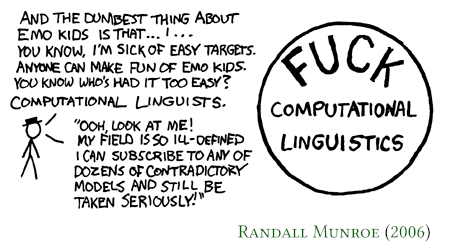
\includegraphics[scale=0.85]{figuras/xkcd.png} }
\nocite{xkcd}
\label{xkcd}
% Esta seção é opcional e fica numa página separada; ela pode ser usada para
% uma dedicatória ou epígrafe.
\end{dedicatoria}

% Reinicia o contador de páginas (a próxima página recebe o número "i") para
% que a página da dedicatória não seja contada.
\pagenumbering{roman}

% Agradecimentos:
% Se o candidato não quer fazer agradecimentos, deve simplesmente eliminar
% esta página. A epígrafe, obviamente, é opcional; é possível colocar
% epígrafes em todos os capítulos. O comando "\chapter*" faz esta seção
% não ser incluída no sumário.
\chapter*{Agradecimentos}
% \epigrafe{Do. Or do not. There is no try.}{Mestre Yoda}

Gostaria de agradecer à minha família pelo apoio e sustento que me proporcionaram ao longo dessa longa jornada como mestrando. Especialmente meu primo, David Barzilai, que me acompanhou enquanto eu escrevia parte dessa tese e até me abrigou em sua casa por uns dias enquanto eu terminava mais uma versão do texto.

Ainda sobre abrigo, gostaria de agradecer meu amigo Lucas Magno por sempre me receber de portas abertas em sua sala. A vida acadêmica pode ser bem solitária, mas sempre ter com quem bandejar certamente ajuda.

Gostaria também de agradecer meus amigos Mauricio, Zeca e a família deles\footnote{Menos a gata Gigi} por sempre me receberem e me alimentarem quando eu ia passar o dia trabalhando lá. Não sei o por que eles achavam tão razoável e normal eu ir lá com tanta frequência mas sou muito grato por isso.
Além de me receberem, eles auxiliaram essa tese de diversas formas diretas e indiretas; por exemplo, o Zeca, a Lira e a Júlia Rissin me resgataram de carro uma madrugada quando fiquei ilhado no meio do nada voltando da casa deles. E ainda quando o Mauricio resgatou todos os dados perdidos do HD quando o disco \texttt{sdb} da máquina ratel faleceu com o ``tec-tec da morte''.

Falando na ratel, gostaria de agradecer ao Sergio Ricardo Milare e ao William Alexandre Miura Gnann da seção de informática do IME pela ajuda com essa máquina e em recuperar a última versão do meu código que eu tinha esquecido de dar \texttt{git push}. Tecnicamente a ratel nem era responsabilidade deles então sou muito grato por sempre serem tão solícitos e não só ignorarem nossos emails falando que eu quebrei a ratel de novo. 

Gostaria de aproveitar para também agradecer a equipe dos restaurantes universitários, equipes de limpeza da USP, responsáveis da sala do chá do IME, a secretaria da pós do IME, o Renato Geh, Felipe "Sub" Serras e demais RDs e representantes do corpo estudantil, o Nelson Lago, o professor Carlinhos (que me fez desistir das minhas ideias ruins e só entrar no mestrado do IME logo) e todos os outros funcionários e professores do IME e da USP que me proporcionaram as condições de desenvolver esse projeto.


Não posso deixar de agradecer meu querido orientador Marcelo Finger que sempre me deu muita liberdade e apoio ao longo do projeto, sempre trazendo novas ideias e oportunidades para mim.

Gostaria de agradecer a Júlia Rissin também pela ajuda com os gráficos, me salvando de apresentar uma tese cheia de \textit{printscreens}.


Gostaria também de agradecer todos os meus amigos e colegas que fizeram parte dessa minha jornada do mestrado, como o Gabriel Morete, Lucas Arenstein, Thiago Lima, Rebecca Helena, Pedro Souza (cara mais fascinado por \texttt{git} que eu já vi), Thiago Tarraf Varella, Estêvão, Pedro Bruel, Rodrigo Berezovsky, Arieh Szafir Goldstein, Matheus Castello, Roger Bravo, e meu colegas do LIAMF, por conta da pandemia nossa convivência foi curta mas foi um prazer conhecer todos vocês.


Por fim gostaria de agradecer meu grande amigo Patrick Eli Catach. Por conta da distância entre a Inglaterra e o Brasil as oportunidades de nos vermos são raras, mas isso nunca o impediu de se interessar pelo meu trabalho --- às vezes até mais do que eu --- e de sempre ser o primeiro a querer ler meus rascunhos incompletos.
Seu apoio foi muito importante para mim e para esse projeto, seja me recebendo nas suas raras visitas ao Brasil ou quando ele veio me visitar na Holanda e passamos boa parte do tempo discutindo meu projeto, silenciosamente trabalhando lado a lado ou até mesmo vindo me cobrar de mandar minha tese para ele ler. Para ele, a maioria desses acontecimentos devem ter sido corriqueiros e sem muito significado, mas para um amigo que mora tão longe e que poderia ter facilmente acabado se afastando e perdendo o contato ao sair do país --- como aconteceu com tantos outros no meio desse êxodo acadêmico --- sua dedicação e sinceridade foram extremamente marcantes. 

\textit{I would also like to thank Minaksie Ramsoekh for all the help in getting to Delft and during my stay there.}


\textit{They say science is built on-top of the shoulders of giants, however due to an archaic publishing model and corporate greed most of the population has no access to these giants to even attempt to climb on-top of them. That is why I would like to thank everyone involved in the dissemination of free and open science and in particular to Alexandra Elbakyan and her project Sci-Hub which was essential in the realization of this thesis.}


%!TeX root=../tese.tex
%("dica" para o editor de texto: este arquivo é parte de um documento maior)
% para saber mais: https://tex.stackexchange.com/q/78101

% As palavras-chave são obrigatórias, em português e em inglês, e devem ser
% definidas antes do resumo/abstract. Acrescente quantas forem necessárias.
\palavrachave{Aprendizado de Máquina}
\palavrachave{Refatoração}
\palavrachave{Processamento de Linguagem Natural}
\palavrachave{Engenharia de Software}


\keyword{Machine Learning}
\keyword{Code Refactoring}
\keyword{Natural Language Processing}
\keyword{Software Engineering}


% O resumo é obrigatório, em português e inglês. Estes comandos também
% geram automaticamente a referência para o próprio documento, conforme
% as normas sugeridas da USP.
\resumo{
Técnicas de processamento de linguagem natural podem ser aplicadas aos mais diversos textos, não somente àqueles redigidos em  linguagens humanas como também àqueles redigidos em linguagens ditas artificiais, como códigos escritos em linguagens de programação.
Refatoração de código é uma técnica fundamental em engenharia de software, sendo utilizada tanto como uma ferramenta para garantir a qualidade do código como também como um passo importante na expansão de funcionalidades e depuração.
Nesse trabalho propomos um modelo para refatoração automática de código. Ao utilizar diretamente o código fonte como entrada em nosso modelo de processamento de código nós obtemos automaticamente sugestões de refatorações do tipo extração de função. 
O modelo proposto consiste em uma rede neural capaz de receber uma representação vetorial do código a ser refatorado e gerar uma representação da refatoração sugerida.
Essa rede foi treinada com base numa lista de repositórios de código obtida através de uma colaboração com a TU Delft na Holanda. Com base nessa lista foi criado o maior dataset de refatorações de extração de função existente --- até o momento da publicação dessa tese --- sendo 60\% maior do que o segundo maior dataset de seu tipo. Além disso, nosso modelo final atingiu uma acurácia de teste de 0.7275.
}

\abstract{
Natural Language Processing techniques can be applied to text in general, not only to human language but also to artificial languages such as software code. Code refactoring is a fundamental software engineering technique used both as a quality assurance tool and an important step in code correction and functionality enhancement. 
In this work, we propose a novel code refactoring model.
By utilizing source code as input to our model we obtain automated suggestions of function extraction code refactoring in order to achieve better readability and attain good practices in general. The proposed model consists of a neural network that receives a vectorial representation of the source code and outputs a representation of the suggested refactored code. This network was trained based on a list of repositories provided through a collaboration with TU Delft Holland. Based on this list we created the biggest existing function extraction refactoring dataset --- as of the time this thesis was presented --- being \%60 bigger than the second biggest dataset of its type. Furthermore, our final model achieved a test accuracy of 0.7275.
}




%%%%%%%%%%%%%%%%%%%%%%%%%%% LISTAS DE FIGURAS ETC. %%%%%%%%%%%%%%%%%%%%%%%%%%%%%

% Como as listas que se seguem podem não incluir uma quebra de página
% obrigatória, inserimos uma quebra manualmente aqui.
\makeatletter
\if@openright\cleardoublepage\else\clearpage\fi
\makeatother

% Todas as listas são opcionais; Usando "\chapter*" elas não são incluídas
% no sumário. As listas geradas automaticamente também não são incluídas por
% conta das opções "notlot" e "notlof" que usamos para a package tocbibind.

% Normalmente, "\chapter*" faz o novo capítulo iniciar em uma nova página, e as
% listas geradas automaticamente também por padrão ficam em páginas separadas.
% Como cada uma destas listas é muito curta, não faz muito sentido fazer isso
% aqui, então usamos este comando para desabilitar essas quebras de página.
% Se você preferir, comente as linhas com esse comando e des-comente as linhas
% sem ele para criar as listas em páginas separadas. Observe que você também
% pode inserir quebras de página manualmente (com \clearpage, veja o exemplo
% mais abaixo).
\newcommand\disablenewpage[1]{{\let\clearpage\par\let\cleardoublepage\par #1}}

% Nestas listas, é melhor usar "raggedbottom" (veja basics.tex). Colocamos
% a opção correspondente e as listas dentro de um grupo para ativar
% raggedbottom apenas temporariamente.
\bgroup
\raggedbottom

%%%%% Listas criadas manualmente

\chapter*{List of Abbreviations}
% \disablenewpage{\chapter*{Lista de abreviaturas}}

\begin{tabular}{rl}
    NLP & Natural Language Processing \\
    ML & Machine Learning \\
    LSP & Language Server Protocol \\
    AST & Abstract Syntax Tree \\
    DFA & Discrete Finite Automata \\
    GloVe & Global Vectors (for Word Representation) \\
    SQuAD & Stanford Question Answering Dataset  \\
    BERT & Bidirectional Encoder Representations from Transformers \\
    SBERT & Sentence-BERT \\
    RoBERTa & Robustly optimized BERT approach \\
    ALBERT & A Lite BERT \\
    QA & Question Answering \\
    dbmc1 & distiluse-base-multilingual-cased-v1 \\
    Ptr-Net & Pointer Network \\
    RNN & Recurrent Neural Network \\
    LSTM & Long Short-Term Memory \\
    TPE & Tree-structured Parzen Estimator \\
    Acc & Accuracy \\
    Val & Validation \\
    IDE & Integrated Development Environment \\
    ORM & Object Relational Mapping  \\
    FAPESP & São Paulo Research Foundation (Fundação de Amparo à Pesquisa do Estado de São Paulo) \\
    BEPE & Grant for Research Abroad (Bolsa Estágio de Pesquisa no Exterior) \\
    TUDelft & Delft University of Technology (Technische Universiteit Delft) \\
    SERG & Software Engineering Research Group\\
\end{tabular}

%\chapter*{Lista de símbolos}
% \disablenewpage{\chapter*{Lista de símbolos}}

% \begin{tabular}{rl}
%   $\omega$ & Frequência angular\\
%     $\psi$ & Função de análise \emph{wavelet}\\
%     $\Psi$ & Transformada de Fourier de $\psi$\\
% \end{tabular}

% Quebra de página manual
\clearpage

%%%%% Listas criadas automaticamente

% Você pode escolher se quer ou não permitir a quebra de página
\listoffigures
% \disablenewpage{\listoffigures}

% Você pode escolher se quer ou não permitir a quebra de página
\listoftables
% \disablenewpage{\listoftables}

% Esta lista é criada "automaticamente" pela package float quando
% definimos o novo tipo de float "program" (em utils.tex)
% Você pode escolher se quer ou não permitir a quebra de página
% \listof{program}{\programlistname}
\renewcommand\listoflistingscaption{List of Programs}
\listoflistings
% \disablenewpage{\listof{program}{\programlistname}}

% Sumário (obrigatório)
\tableofcontents

\egroup % Final de "raggedbottom"


% Referências indiretas ("x", veja "y") para o índice remissivo (opcionais,
% pois o índice é opcional). É comum colocar esses itens no final do documento,
% junto com o comando \printindex, mas em alguns casos isso torna necessário
% executar texindy (ou makeindex) mais de uma vez, então colocar aqui é melhor.
% \index{Inglês|see{Língua estrangeira}}
% \index{Figuras|see{Floats}}
% \index{Tabelas|see{Floats}}
% \index{Código-fonte|see{Floats}}
% \index{Subcaptions|see{Subfiguras}}
% \index{Sublegendas|see{Subfiguras}}
% \index{Equações|see{Modo matemático}}
% \index{Fórmulas|see{Modo matemático}}
% \index{Rodapé, notas|see{Notas de rodapé}}
% \index{Captions}
% \index{Versão original|see{Tese/Dissertação, versões}}
% \index{Versão corrigida|see{Tese/Dissertação, versões}}
% \index{Palavras estrangeiras|see{Língua estrangeira}}
% \index{Floats!Algoritmo|see{Floats, ordem}}


%%%%%%%%%%%%%%%%%%%%%%%%%%%%%%%% CAPÍTULOS %%%%%%%%%%%%%%%%%%%%%%%%%%%%%%%%%%%%%

% Aqui vai o conteúdo principal do trabalho, ou seja, os capítulos que compõem
% a dissertação/tese. O comando mainmatter reinicia a contagem de páginas,
% modifica a numeração para números arábicos e ativa a contagem de capítulos.
\mainmatter

\pagestyle{mainmatter}

% Espaçamento simples
\singlespacing



%!TeX root=../tese.tex
%("dica" para o editor de texto: este arquivo é parte de um documento maior)
% para saber mais: https://tex.stackexchange.com/q/78101

\chapter{Introduction}
\label{chap:intro}



What is the difference between computer science and software engineering? Both deal with computers, right? Are they not the same thing?

Computer science is the field focused on the theoretical powers of computers and the algorithms we write for them. Is this problem decidable? NP-complete? Can this thing be considered a Turing machine? Is P=NP? What functions can be approximated by neural networks? How can we color, with the minimal number of colors,  the vertices of a graph so that no two adjacent vertices have the same color? There are a myriad of important and interesting questions posed in this large field of study, but they are all centered around the computers and the theoretical.

This is where the computer science and software engineering fields differentiate themselves. Whereas one field is centered around computers and algorithms, the other is centered around the humans using these computers and implementing those algorithms, or to be more precise the relation and interactions between programmers and their code.

Software engineering is the field concerned with more mundane and practical aspects of programming, when we speak of code complexity we are talking about a more abstract concept than the well defined time complexity so ubiquitous in computer science theory, we are talking about the \textit{perceived} complexity of a program\footnote{This is not to say that software engineers have no interest in or knowledge of the theoretical aspects of computer science or that the two fields are completely disjoint, the best developers would take into account both the code's time complexity and its perceived complexity when writing a program.}. How easy is it to maintain? Is it readable? Can we easily test it for limit cases where bugs may be hiding? Is there code duplication that could be simplified?


Software engineering is the field of study concerned with the efficiency of the programmers and their code, not simply their code. How can we decrease the implementation time of a new feature and make developers more efficient? What are the bottlenecks in development? How do the developers organize themselves? What if they are part of a team? What about their code base? How do we measure the quality of a piece of code in regards to the value it brings to our clients or even to our own developers?

When trying to add a new feature to an existing software, a common first step is the re-writting of existing code, not the creation of new code as one might expect \citep{martinfowler}. The field of software engineering has a special name for this re-writting step, it is called \textit{refactoring}. To refactor a piece of code is to make simple and incremental changes in order to make it easier to work with and to be expanded upon. A survey from \citet{1001} shows that refactorings are a key element in the software development cycle. As can be seen in Figs.~\ref{fig:pizzas}, nearly four out of five developers in the 1,183 developers surveyed indicated that they refactored code every week or even almost every day. Two-thirds of these respondents said that they had refactoring sessions of an hour or longer during this time.



\begin{figure}
\centering
\begin{subfigure}{.5\textwidth}
  \centering
  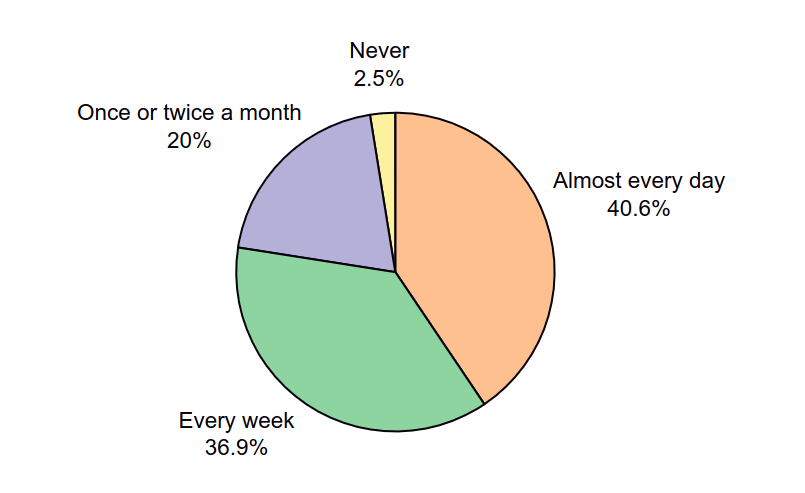
\includegraphics[width=1.2\linewidth]{figuras/q1pizza.png}
  \caption{In the past month, how
often have you performed any code refactoring? (Out of 1,181
respondents)}
  \label{fig:q1}
\end{subfigure}
\begin{subfigure}{.5\textwidth}
  \centering
  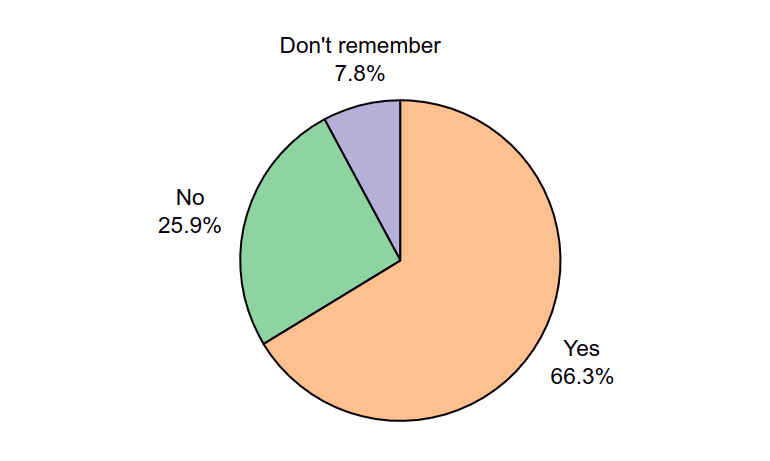
\includegraphics[width=1.2\linewidth]{figuras/q2pizza.png}
  \caption{During this time, did you ever refactor code for an hour or more in a single session? (Out of 1,145 respondents)}
  \label{fig:q2}
\end{subfigure}
\caption{Pie graphs of two of the 20 questions about refactoring answered by a group of 1,183 developers that were paying subscribers of IntelliJ Platform based IDEs. \citep{1001}}
\label{fig:pizzas}
\end{figure}


As one might expect from such an integral part of the software development cycle, extensive work \citep{1001, 7vista, abid202030} has been done to better understand how and when refactorings are done, or how to optimize and automate this often manual and repetitive task.
However, much of the work done is in order to automate a refactoring after a developer detected an opportunity and it is mediated by said developer. Let's say we want to break a long function into smaller functions, the developer has to go to the function and select the line span that they wish to extract.
The onus of refactoring the code is still on the developer, it is certainly faster than doing it manually without the help of these small automations but there is still room for improvement. Taking the same example as before, it would be even better if the IDE could suggest to the programmer which functions could use a refactoring or even which lines should be extracted. We posit that by making the refactoring process more automated and less reliant on the developer, refactoring would become even more commonplace and make developers in general more productive.

But how exactly could we achieve such automation? That is what we hope to answer in detail in the following chapters of this thesis dissertation. We intend to leverage the \textit{naturalness} of programming languages to train a machine learning model based on existing natural language processing techniques to automate refactorings of the function extraction type.


One might ask what is the ``naturalness of a programming language'' and why should we use NLP techniques in languages that are, by their very definition, non-natural but first we need to address what even is a natural language. 

The concept of natural language could be defined by what they are not: they are not artificially constructed and they are not ``rigid''. Let us take \citet{lang_file} definition of natural languages:


\begin{myquote}   
\textit{All languages exhibit all nine design features} \textbf{{\small
[as defined by \citet{hockett1960origin}:
Mode of Communication, Semanticity, Pragmatic Function, Interchangeability, Cultural Transmission, Arbitrariness, Discreteness, Displacement, Productivity]
}
} \textit{any communication system that does not is therefore not a language. Furthermore, as far as we know, only human communication
systems display all nine design features.} \textbf{[...]}

\qquad \textit{Because all languages exhibit the nine design features, does this mean that any communication system that exhibits all nine features should be considered a language? 
For example, there are formal languages, such as the formal logic used to write mathematical proofs and various computer languages. While these formal languages display all of the design features, they nevertheless differ in critical ways from languages such as English, Spanish, Mandarin, and Apache. For example, no child could ever acquire a computer language like C++ as his native language! 
Furthermore, a number of people engage in constructing languages that imitate human language as a hobby. There are many reasons that people might choose to do this. For example, the created language could be used in some sort of fictional universe, such as Klingon in the television series Star Trek or Dothraki and Valyrian in the series Game of Thrones. Or it might be designed to facilitate international communication, which was the goal of the designers of the language Esperanto. Other people, such as J.R.R. Tolkien, have constructed artificial languages just for fun.}
\par
\qquad \textit{Do we want to make a distinction between languages such as English, Spanish, Mandarin, and Apache, on the one hand, and Esperanto, Elvish, Dothraki, Valyrian, and Klingon, on the other? And how should we classify `formal' languages?
Although many of these questions are still open to debate and research, we will make the following distinctions }
\textbf{[...]}
\textit{we call natural languages, those languages that have evolved naturally in a speech community. The lexicon and grammar of a natural language have developed through generations of native speakers of that language. A constructed language, on the other hand, is one that has been specifically invented by a human and that may or may not imitate all the properties of a natural language.} \\\citet{lang_file}
\end{myquote}


Essentially, natural languages are languages that changed and evolved naturally alongside humans and are used for communication. That is not to say that a constructed language cannot become a natural language, an example is Modern Hebrew which was reconstructed and expanded from Ancient Hebrew (a liturgical and dead language) and then adopted by a particular community\footnote{The matter of Modern Hebrew's ``creation'', ``revival'' or ``(Re)vernacularization''\citep{spolsky1995conditions} and its characterization as a constructed language is a point of contention, this discussion is out of the scope of this work but we refer readers interested in a primer on the subject to \citet{izre2003emergence}.}.
We used non rigid to describe natural languages because of this capacity to change and evolve as well as its semantical robustness, even if a text contains a few mistakes its meaning may still be grasped while programming languages are brittle to mistakes (e.g. typos in variable names or parameter order inversion can drastically change the meaning of code or even break it).

\citet{lang_file} also brings us a sort of definition for formal languages:

\begin{myquote}
\textit{The distinction between constructed languages and formal languages is that formal languages are not the sort of system that a child can acquire naturally.} \\\citet{lang_file}
\end{myquote}


Although this is not wrong, most computer scientists would find it lacking as a definition. A more common formulation would be to define it as the set of all strings that can be derived from a formal grammar. That is to say, a formal language is defined (or generated) by its grammar and a piece of text can be identified as part of a formal language if it can be ``recognized'' by its grammar (i.e. parsed). More formally, a generative grammar is defined by a 4-tuple $(N, \Sigma, P, S)$ where $N$ is the set of non-terminal symbols, $\Sigma$ the set of terminal symbols (disjoint of $N$), $P$ the set of production or generation rules and $S$ the sentence or start symbol.

Table~\ref{table:grammar} depicts an example of the production rules part of a formal grammar for syntactically correct infix algebraic expressions for three variables, namely x, y and z, and depicts Fig~\ref{fig:parsetree} an example of a parse tree generated with these production rules for the expression $(x + y) \times x - z \times y / (x + x)$.


\begin{figure}[!ht]
\centerline{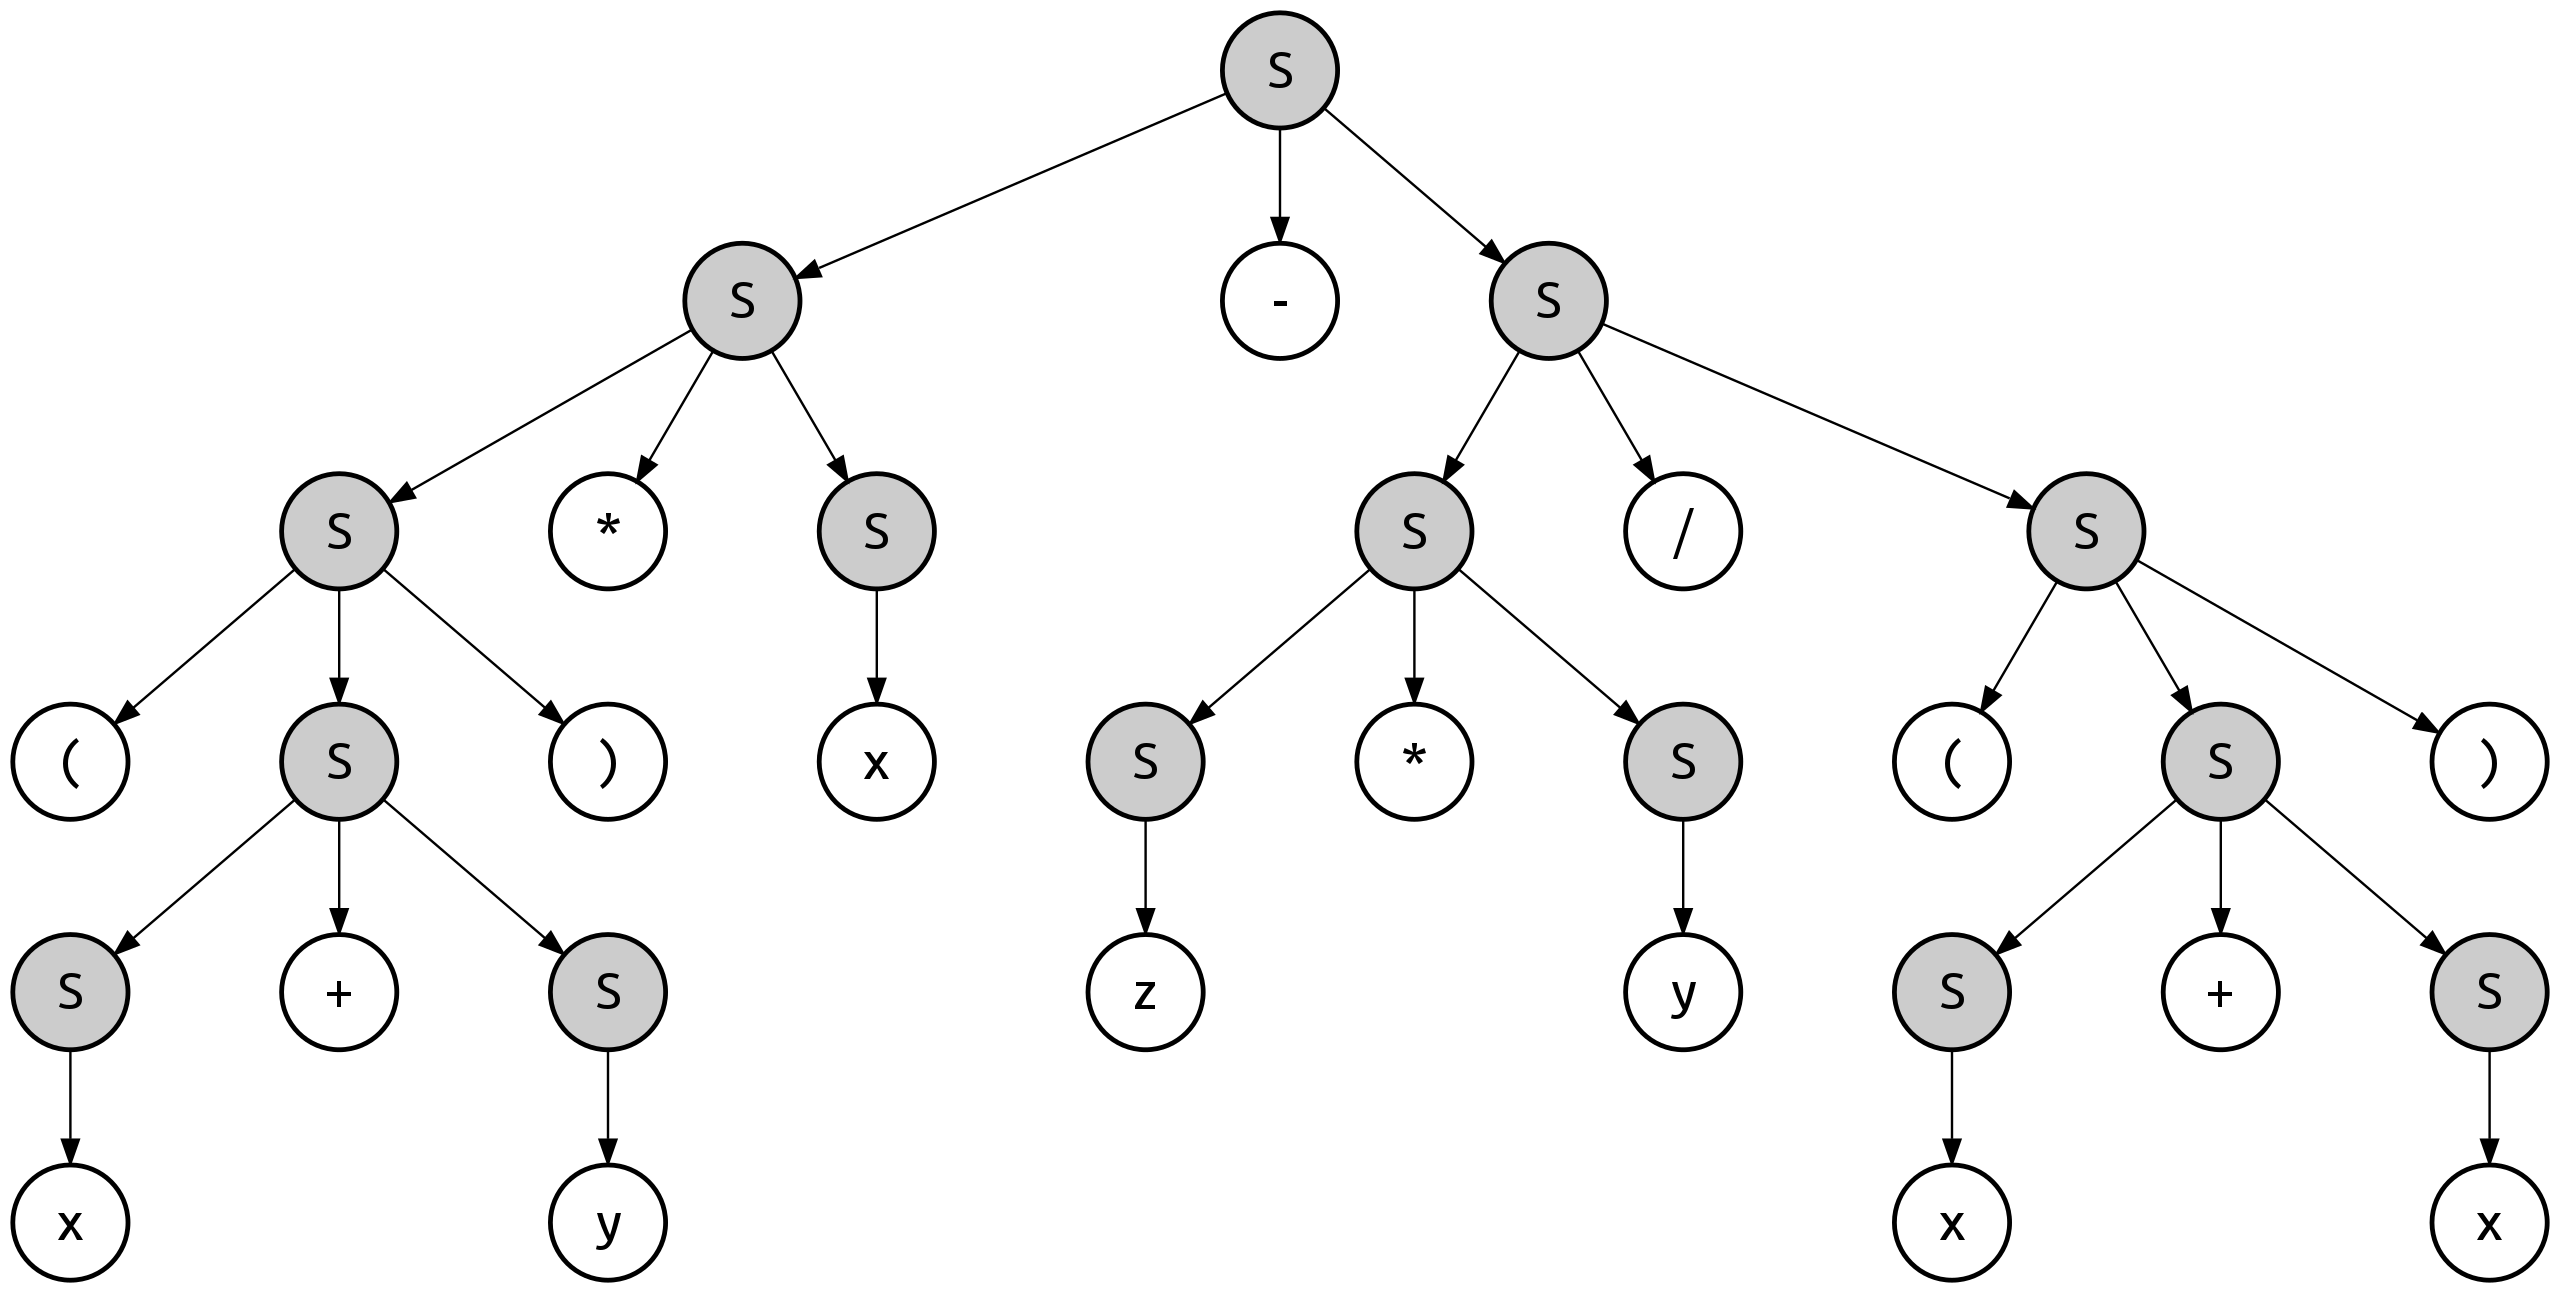
\includegraphics[width=\textwidth]{figuras/parse_tree_grammar.png}   }
\caption{One of the possible parse trees for the expression $(x + y) \times x - z \times y / (x + x)$ created from the production rules in Table~\ref{table:grammar}. Image from \citet{parse_tree}.}
\label{fig:parsetree}
\end{figure}

\begin{table}[]
\begin{tabular}{llll}
$S \rightarrow x$   &&& $S \rightarrow S + S$      \\
$S \rightarrow y$   &&& $S \rightarrow S - S$      \\
$S \rightarrow z$   &&& $S \rightarrow S \times S$ \\
$S \rightarrow (S)$ &&& $S \rightarrow S / S$     
\end{tabular}
\caption{Production rules of a formal grammar for syntactically correct infix algebraic expressions for three variables, namely x, y and z. In essence, the grammar is defined by these 8 production rules forming the $P$ set, $\{x, y, z, +, -, (, ), \times, /\}$ as the terminal symbols set $\Sigma$, $\{S\}$ as the set of non-terminal symbols $N$ and $S$ as the start symbol. Note that this grammar is ambiguous so it has multiple possible parse trees. }
\label{table:grammar}
\end{table}


Formal languages, such as programming languages, can still change and evolve, however this happens as punctuated changes (e.g. the release of Python 3 to substitute Python 2 and the sub-sequential break of compatibility) and in contrast to natural languages that work in a bottom up fashion through social dynamics \citep{croft2008evolutionary}, programming languages are designed top-down by a few designers for many users.

These are not their only differences, another example is that it is not clear if it is feasible to create a translation between natural languages such that the meaning is completely preserved\footnote{And also highly dependent on the definition of \textit{meaning} being used.}. However every mainstream\footnote{There are programming languages that are not developed with universal computation in mind, such as the BlooP \citep{bloop} and Charity \citep{charity} languages, however they are not widely adopted in the industry nor posses a sizable user base.} programming language is Turing complete \citep{turing} so it is always possible\footnote{Anyone who has worked in code translation may tell you that this can be ``easier said than done''. Code portability can be a challenging subject even if we ignore unusual Turing complete languages such as Microsoft's PowerPoint \citep{ppt}.} to exactly translate a piece of code from one language to another.

Nevertheless machine translation between natural languages is an ever thriving research topic. Furthermore, in recent years the area of NLP has seen explosive growth together with new neural network architectures (GRU \citep{GRU}, Transformers \citep{attention_is_all_you_need}, ELMo \citep{ELMo}, BERT \citep{BERT} to name only a few recent ones) and a skyrocketing success reaching even mainstream popularity through large language models such as GPT-4 \citep{gpt4} and LLaMA \citep{llama}. On the other hand, the use and success of machine learning models for analogous tasks in programming languages (e.g. translation between programming languages or transpilation) has been comparatively moderate so far.



Despite having several differences, natural and programming languages also share a series of particularly interesting commonalities that allow the application of models and techniques originally devised for NLP tasks into analogous programming language processing tasks.






This idea is succinctly defined in the naturalness hypothesis:


\begin{myquote}
\textbf{Naturalness Hypothesis. }
\textit{
Software is a form of human communication; software corpora have similar statistical properties to natural language corpora; and these properties can be exploited to build better software engineering tools.}  \\\citet{allamanis2018survey}
\end{myquote}

This insight that programming may be seen as a form of human communication is not by any means new and can be traced back to Donald E. Knuth concept of \textit{literate programming} from his titular work Literate Programming:

\begin{myquote}
\textit{I believe that the time is ripe
for significantly better documentation of programs, and
that we can best achieve this by considering programs
to be works of literature. Hence, my title: `Literate
Programming.'}
\\
\\
\qquad\textit{ Let us change our traditional attitude to the construction of programs: Instead of imagining that our
main task is to instruct a computer what to do, let us
concentrate rather on explaining to human beings what
we want a computer to do.}
\\
\\
\qquad \textit{The practitioner of literate programming can be regarded as an essayist, whose main concern is with exposition and excellence of style. Such an author, with
thesaurus in hand, chooses the names of variables carefully and explains what each variable means. He or she strives for a program that is comprehensible because its
concepts have been introduced in an order that is best
for human understanding, using a mixture of formal
and informal methods that re{\"i}nforce each other. }\\\citet{knuth1984literate}\end{myquote}


Although the naturalness hypothesis may not seem surprising to some, it is worth understanding the genesis of this naturalness. 

As stated by \citet{allamanis2018survey} ``\textit{naturalness of code seems to have a strong connection with the fact that developers prefer to write \citep{Allamanis_2014} and read \citep{7180076} code that is conventional, idiomatic, and familiar because it helps understanding and maintaining software systems}''.

This leads to the idea that code artifacts may contain recurring and predictable patterns that can be leveraged by machine learning models to perform a plethora of different tasks, in a not dissimilar way to how recurring and predictable patterns in linguistic corpora have been successfully utilized in NLP models.

\citet{naturalidade_original} demonstrated that corpus-based statistical language models can capture a high level of regularity in software, even more so than in english, and that this is not an artifact of the programming language syntax but rather it arises from the naturalness of the code.

They reason that, like natural languages, software is repetitive and predictable:

\begin{myquote}
    \textit{We begin with the conjecture that \emph{most software is also natural}, in the sense that it is created by humans at work, with all the attendant constraints and limitations} \textbf{[...]}
    \\
    \\
    \qquad \textit{Programming languages, in theory, are complex, flexible and powerful, but the programs that \underline{real} people \underline{actually} write are mostly simple and rather repetitive, and thus they have usefully predictable statistical properties that can be captured in \underline{statistical language models} and leveraged for software engineering tasks. }\\\citet{naturalidade_original} 
\end{myquote}

An important point raised was that \textbf{most} software is also natural, not all code ever written. One could easily argue that the hypothesis of human communication can be discarded when we are dealing with esoteric programming languages such as brainfuck \citep{brainfuck}, Piet \citep{piet} or Malbolge \citep{malbolge}, aptly named after the 8th circle of Hell from \citet{alighieri1788divina}. Fig.~\ref{fig:eso} presents three code snippets to help clarify how convoluted and deliberately obtuse esoteric languages can be designed to be. 
Being less extreme, not all code could be said to be ``readable'' or to be clearly and well structured, e.g. an inexperienced programmer's code\footnote{Recent evidence actually suggests that the amateur nature of inexperienced programmers may actually be beneficial for the corpus as was described in testimony given by Replit’s Head of AI in \citet{podcast_replit}, where they claim to have obtained a 50\% increase in performance when fine tuning their model on the replit codebase --- which contains a lot of code from people still in the process of learning how to program. However, our point stands that even if not all code could be considered natural it is likely relegated to a small part of softwares at large and would end up as an issue of data quality the same way data quality is an issue for NLP corpora.}, may not conform to best practices and contain confusing or out-write miss-leading function and variable names. If this is sufficient to classify the code as not natural is a matter out of the scope of this project, however we posit that those are rare instances in large successful projects that usually have naming conventions, contributing guidelines and code quality metrics and as such would not have a huge impact on data quality and training performance.

\begin{figure}[!ht]
\centerline{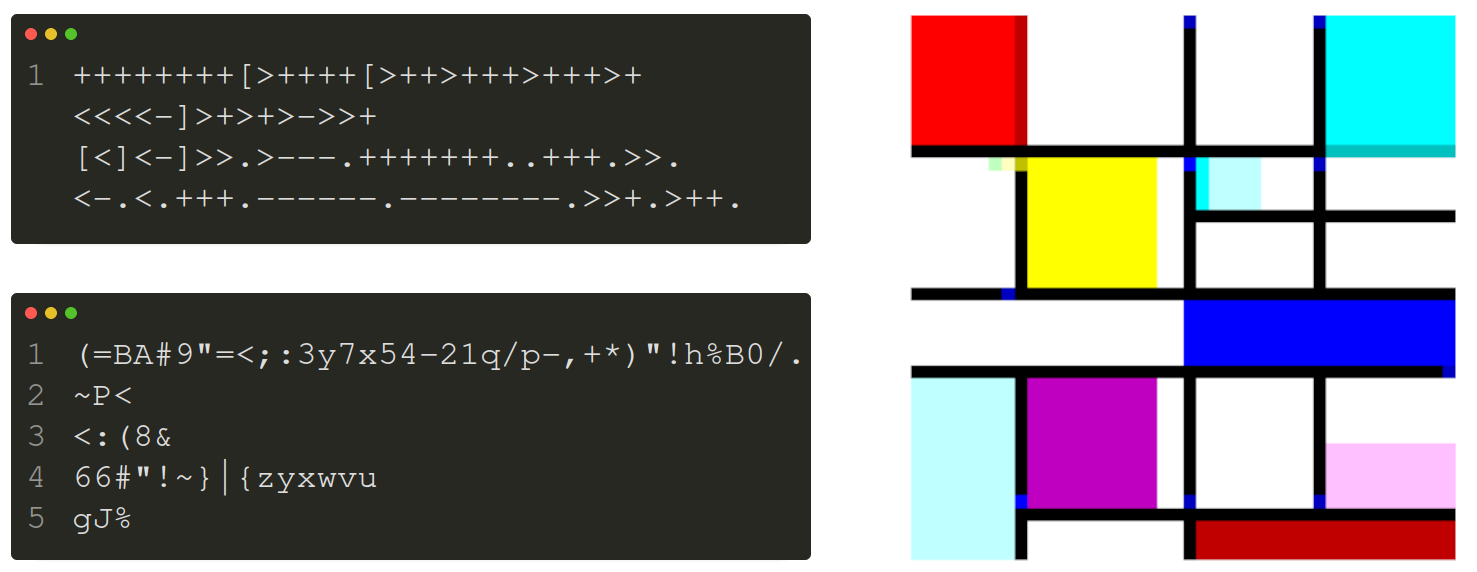
\includegraphics[width=\textwidth]{figuras/eso.png}   }
\caption{3 code snippets in esoteric languages. On the right the image that resembles a painting from Piet Mondrian is a program in the Piet language that prints the ``Piet'' string \citep{piet_image}. On the upper left is a ``Hello World!'' program written in brainfuck where only 8 characters (><+-.,[]) are available and each correspond to a different pointer operation \citep{brainfuck_codigo}. Lastly, on the lower left we have a \texttt{cat} program (that does not stop at EOF) written in Malbolge, a language designed to be as difficult to program in as possible with a ternary system, self-altering code and, once again, only 8 valid instructions \citep{malbolge_codigo}.}
\label{fig:eso}
\end{figure}



So far, this naturalness approach to programming languages has been shown to be fruitful many times. \citet{allamanis2018survey} make an extensive review of the literature compiling works that leverage in some way the ideas behind the naturalness hypothesis, there are too many to list here so we encourage interested readers to seek the original paper that is readily available online. Readers pressed for time may be interested in inspecting the tables since they compile most of the surveyed work in a systematic and well organized manner. It is important to note that this is not an exhaustive survey since it was published in 2018 and this field of study has by no means stopped since then. Two interesting and more recent works are the code2vec \citep{code2vec}, capable of abstracting the work done by a function by naming it based solely on information obtained through its abstract syntax tree and code2seq \citep{code2seq}, not only capable of predicting method names but also predicting natural language captions given partial and short code snippets, and to even generate method documentation.

We believe these ideas and the results we obtained during the course of this project serve as a proof of the soundness of our approach.


\section{Goals}

This project intends to accomplish two main goals:

\begin{itemize}
\item Understand if deep learning models are capable of predicting fine-grained refactorings, i.e. where exactly the source code should be refactored.
\item Create a model for automated function extraction.
\end{itemize}

\section{Organization}
The thesis is organized as follows: in Chapter~2 we define refactorings and propose a theoretical IDE plugin to better illustrate our objectives as well as provide some software engineering background; in
Chapter~3 we present the theoretical background of our models and other NLP and ML concepts; in Chapter~4 we present related work on automating refactorings; in Chapter~5 we explain how we built our dataset; in Chapter~6 we define the building blocks of our model followed by our experiments with those blocks in Chapter~7; and, finally, in Chapter~8 we give our concluding remarks and trace possible future steps.

%!TeX root=../tese.tex
%("dica" para o editor de texto: este arquivo é parte de um documento maior)
% para saber mais: https://tex.stackexchange.com/q/78101

\chapter{An imaginary function extraction plugin}

Although every modern IDE has a series of tools for automating common simple code refactorings, the automation of suggestions of refactorings is still lacking. E.g., renaming a variable can be easily accomplished by tools that scan your program for instances of this variable in the appropriate scope. But there is no efficient tool to our knowledge that automatically detects the need to rename a variable and suggests a new name.

In this chapter we will propose the structure of how one could create an IDE plugin that automates refactorings of the function extraction type and suggests instances of such refactorings. Our objective is by no means the construction nor the implementation of this imaginary plugin, as previously stated in our goals we only intend to create a model that, given only a function definition, is capable of performing a function extraction. We propose this plugin as a mental exercise to clarify some of the practical uses of the work proposed in this project and as a way to introduce software engineering concepts that the readers may need to fully comprehend to understand this project.






\section{Code Refactoring}

This project aims at automating refactorings but we never actually defined what refactoring is, so let us look at some definitions starting with the one who coined the term:

\begin{myquote}
    
\textit{This thesis defines a set of program restructuring operations (refactorings) that support the design, evolution and reuse of object-oriented application frameworks. [...] The refactorings are defined to be behavior preserving, provided that their preconditions are met. Most of the refactorings are simple to implement and it is almost trivial to show that they are behavior preserving.}\\ \citet{opdyke1992refactoring}
\end{myquote}

Another simpler definition from another pioneer on the subject, Martin Fowler, could be useful to those new to the term:

\begin{myquote}
\textbf{Refactoring} (noun): \textit{a change made to the internal structure of software to make it easier to understand and cheaper to modify without changing its observable behavior.} \\\citet{martinfowler}
\end{myquote}
\begin{myquote}
\textbf{Refactoring} (verb): \textit{to restructure software by applying a series of refactorings without changing its observable behavior.} \\\citet{martinfowler}
\end{myquote}


From these definitions we can gather that ideally each refactoring would be a simple and small step that a programmer could take in order to improve the perceived complexity of a program and be more compliant with best practices. After taking a series of these small steps a program will have an improved maintainability, being more readable and easier to debug while behaving the same exact way. Fig.~\ref{ilustracao_refac_func2class} shows an example of such an operation, a refactoring categorized as \textit{Combine Functions into Class}.

\begin{figure}[!ht]
\centerline{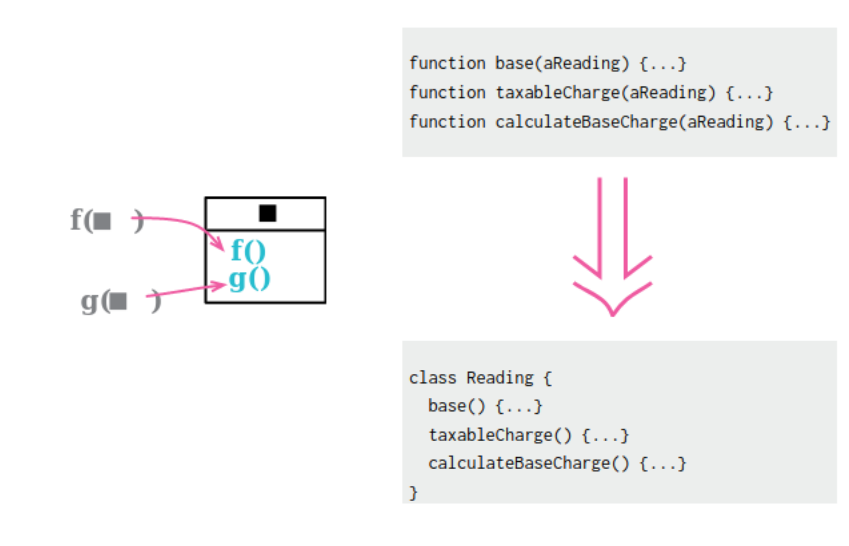
\includegraphics[width=0.8\textwidth]{figuras/class_extract.png}   }
\caption{An instance of the ``Combine Functions into Class'' refactoring. Example extracted from  \citep{martinfowler}.}
\label{ilustracao_refac_func2class}
\end{figure}


However, in practice this definition of refactoring being a behavior-preserving code transformation does not always hold true. It is not uncommon to use the term refactoring in ways that defy its academic definition, Martin Fowler addresses this:



\begin{myquote}
\textit{Over the years, many people in the industry have taken to use `refactoring' to mean any kind of code cleanup---but the definitions above point to a particular approach to cleaning up code. Refactoring is all about applying small behavior-preserving steps and
making a big change by stringing together a sequence of these behavior-preserving steps. Each individual refactoring is either pretty small itself or a combination of small steps. As a result, when I'm refactoring, my code doesn't spend much time in a broken state, allowing me to stop at any moment even if I haven't finished.}
\\
\\
\textit{If someone says their code was broken for a couple of days while they are
refactoring, you can be pretty sure they were not refactoring.}\\\citet{martinfowler}
\end{myquote}








That is to say, colloquially refactoring is often used as something more generic and less rigorous than Opdyke's or Fowler's definitions.
A survey of 328 professional software engineers at Microsoft found that developers do not necessarily consider that refactoring is confined to behavior preserving transformations \citep{7vista}. Furthermore: \begin{myquote}
\textit{[...] 78\% define refactoring as code transformation that improves some aspects of program behavior
such as readability, maintainability, or performance. 46\%
of developers did not mention preservation of behavior,
semantics, or functionality in their refactoring definition
at all. [...]
The following shows a few examples of refactoring
definitions by developers.
\\
\qquad `Rewriting code to make it better in some way.'
\\
\qquad `Changing code to make it easier to maintain. Strictly
speaking, refactoring means that behavior does not change,
but realistically speaking, it usually is done while adding
features or fixing bugs.'} 
\\
\citet{7vista} \end{myquote}


Bearing in mind those different meanings, we will stick to Martin Fowler's definition unless stated otherwise. \citet{catalog} has a catalog where he defines many different types of refactorings but we are interested in automating a specific type of refactoring, the function extraction. When our hypothetical plugin suggests a function extraction to its fictional user it will only suggest the extraction, no feature will be added or subtracted. Further code improvements are out of the scope of this project and are left as possible paths for future work.





Following Martin Fowler's nomenclature system \citep{martinfowler}, in this project we will explore the \textit{function extraction} refactoring in particular, where a long function that does many tasks is broken down into smaller functions, that only do one simple task each, being called one after the other. Each new function created from the larger original one is an instance of a function extraction. It is not uncommon to have a series of function extractions being applied sequentially to a single large function. Fig.~\ref{img:func_exract} gives an example of this refactoring.


\begin{figure}[!ht]
\centerline{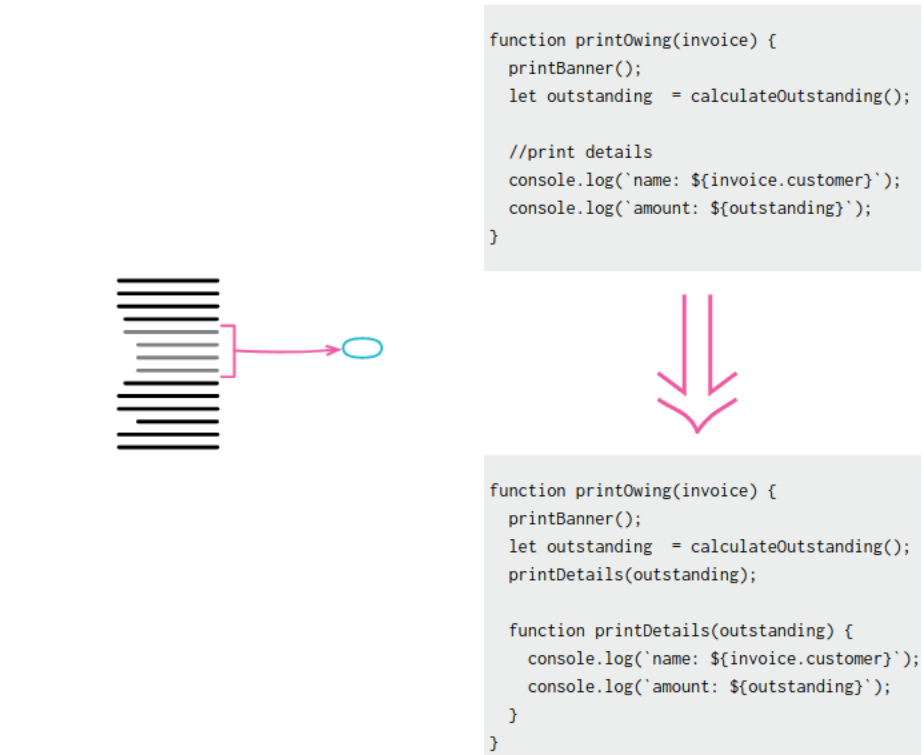
\includegraphics[width=0.8\textwidth]{figuras/func_extract.png}   }
\caption{An instance of the ``Function Extraction'' refactoring. Example extracted from  \citep{martinfowler}.}
\label{img:func_exract}
\end{figure}


\section{The Plugin}

With a clear definition of what is a refactoring and of our objectives we will explore our theoretical plugin and how it could be built. Fig.~\ref{img:plugin} presents the outline of how this plugin would work.

\begin{figure}[!ht]
\centerline{
\includegraphics[width=1.1\textwidth]{figuras/plugin.drawio.png}   }
\caption{Outline of our imaginary plugin broken down into three different parts.}
\label{img:plugin}
\end{figure}



\subsection{Detecting Refactoring Opportunities} 
\label{sec:code_metrics}

As previously stated, code refactoring is not a new subject, extensive work has already been done to classify different types of refactorings. Furthermore, there are no lack of tools \citep{bavote_smell,bavota_smell2,jdeodorant,dig_smells} to identify \textit{code smells} \citep{martinfowler}, a common pattern that may serve as an indication of a deeper problem in the way the system is structured and the need of refactoring. For example a really long function may indicate the need for a function extraction refactoring. 

There are many approaches one could take in order to identify refactoring opportunities. One approach could be to leverage said code smells and their vast literature, another way could be to construct heuristics utilizing a set of code complexity metrics.


There are quite a few metrics that aim at measuring the perceived complexity of a piece of code --- not in the sense of \textit{execution time complexity} but in the sense of \textit{readability and maintainability}. By looking solely at the source code, without executing it, it is possible to provide an estimation of the quality of the software. Some metrics can be more specific and restrictive in their use, for example being tailored to a single programming paradigm (e.g. this suite of metrics designed for Object Oriented programming \citep{OO_metrics}). Other metrics may try to identify ``code smells'' or be specific to a single programming language \citep{goreport}.


Which of these ideas is the best we cannot say without testing and the results would ultimately be dependent on the implementation of the heuristics, but since we are dealing with an imaginary plugin we are not concerned with such details. We will explore the simple code complexity metric known as \textit{maintainability index} in order to better illustrate this piece of our imaginary plugin.

In section ~\ref{sec:mauricio} we will see another possible approach that utilizes machine learning to detect refactoring opportunities and the refactoring type to be used.

\subsubsection{Cyclomatic complexity}
The cyclomatic complexity proposed in 1976 \citep{cyclomatic}, may be defined as the number of linearly independent paths within a piece of code. A program with no control flow statements (such as loops and conditionals) will have a cyclomatic complexity of 1, a program with one conditional statement $if$ will have cyclomatic complexity of 2, one independent path for a True $if$ statement and another for a False $if$ statement.
Cyclomatic complexity may be used as a bound for the number of necessary unit tests for $100\%$ code coverage and a high cyclomatic complexity may be an indicative of complex nested flow statements.


\subsubsection{Halstead Metrics}
The Halstead metrics where developed in 1977 \citep{halstead} as an attempt to define and analyze static properties of a given software, trying to capture a measure of how difficult it is to write or understand a given piece of code. They also estimate how many bugs are present in a given snippet of code.
Let,
\begin{itemize}
    \item[] $\eta_{1}=$ Number of distinct operators     
    \item[] $\eta_{2}=$ Number of distinct operands
    \item[] $N_{1}=$ Total number of operators
    \item[] $N_{2}=$ Total number of operands
\end{itemize}
Halstead defines volume, difficulty, effort and estimated number of bugs as:
\begin{itemize}
    \item[] $V = (N_{1} + N_{2}) * \lg (\eta_{1} + \eta_{2})$ 
    \item[] $D = \frac{\eta_{1}}{2} * \frac{N_{2}}{\eta_{2}} $
    \item[] $E = D*V$
    \item[] $\hat{B} = \frac{ E^{\frac{2}{3}} } {3000}  $
\end{itemize}

\subsubsection{Maintainability Index}
Throughout the years, the maintainability index formula has been tweaked and refined, but on the original paper \citep{maintainability_index} it was defined as:
$$ MI = 171 - 5.2 * \ln (V)  - 0.23 * G - 16.2 * \ln (LoC) $$
Where $V$ is the Halstead Volume, $G$ is the Cyclomatic Complexity and $LoC$ is the total number of lines of code.
Typical values for the maintainability index range from 0 to 100 with 0 being a hard to maintain code and 100 being a well structured, small and easy to maintain code.


\subsection{Refactoring Prediction}

This is the kernel of this plugin and also our main objective in this project. As such, let us treat it as a black box model that simply works until we arrive at Chapter~\ref{chap:models} where we will present our attempts at solving this problem. 


\subsection{Performing Refactorings}
\label{sec:lsp}

Language Server Protocol \citep{lsp}, or LSP as it is commonly referred, was introduced to address the duplication of effort and code across IDE's and text editors. The idea is to create a standard that allows a plugin for a given language (e.g. auto-completion for python) to work in any development tool (e.g. a plugin designed for Atom will work in VSCode) thus reducing the workload of language providers and tooling vendors. Fig~\ref{lsp_image} illustrates this idea.

\begin{figure}[!ht]
\centerline{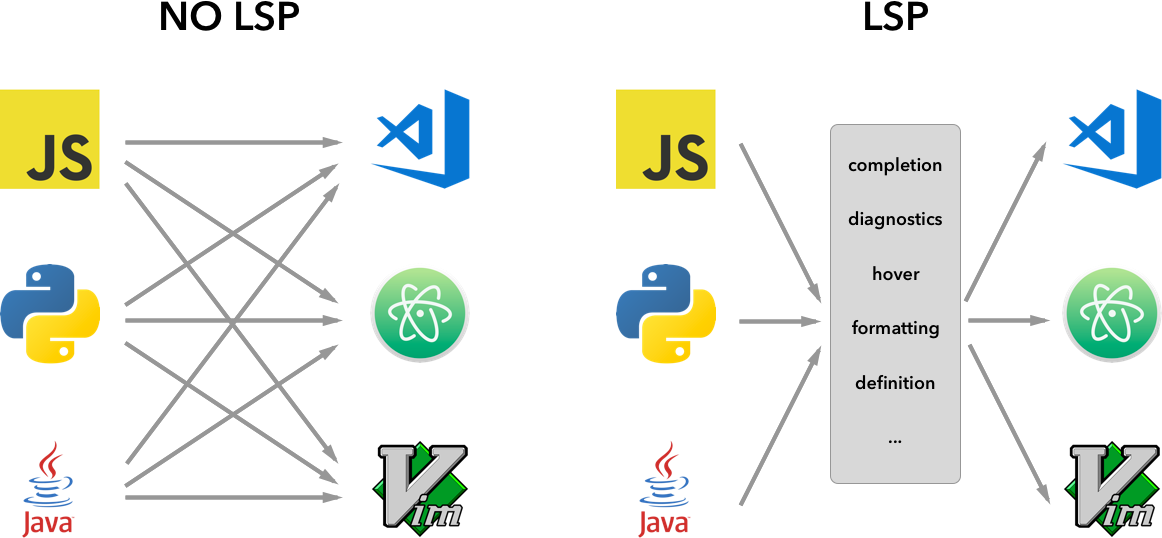
\includegraphics[scale=0.26]{figuras/lsp-ilustracao.png}   }
\caption{An illustration of the problem that LSP was designed to solve. Without LSP we have M languages that need to have support implemented in N different IDE's, but with LSP's we only need to implement support for a language once and it can be re-used anywhere \citep{lsp_ilustracao}.}
\label{lsp_image}
\end{figure}


The goal of LSP is to allow the implementation and distribution of support for a programming language without involving any particular text editor by standardizing  the interaction between the IDE's and the servers that provide language specific features.

With the use of a language server the function extraction refactoring could be easily accomplished by providing the line span to be extracted, in our particular case we could use the Eclipse JDT Language Server \citep{lsp_jdt} to potentially accomplish this for the Java programming language. By describing a refactoring in terms of operations done through the LSP the instructions generated by our model can be easily utilized in any development environment capable of communicating with a language server. It is important to note that function extractions are not always performed with a continuous set of lines which could prove itself a limitation for currently implemented LSP instructions, e.g. the Eclipse JDT Language Server expects a continuous line span. To perform more complex function extractions there may be a need to expand current LSP instruction sets.


%!TeX root=../tese.tex
%("dica" para o editor de texto: este arquivo é parte de um documento maior)
% para saber mais: https://tex.stackexchange.com/q/78101


\chapter{NLP Techniques}
In this chapter we intend to present an overview of some of the NLP concepts, mostly based on neural networks, which are relevant to comprehend this project. As previously mentioned, we intend to leverage NLP techniques to perform the code processing technique of automating function extractions. While some methods can be used as is, others can barely be used at all. In further chapters their usage and limits for our use case will be further explored, while in this chapter they are only going to be introduced to the readers to better situate them.

\section{Embeddings}

When we are dealing with neural networks, we are essentially dealing with matrix operations, so in order to apply NNs to NLP tasks one first needs to somehow transform words and sentences into numbers.


A rudimentary approach would be an one-hot-encoding, where given a vocabulary of size $V$ we have a vector of size $V$ with each word of the vocabulary being associated to a specific index of our vector in a one-to-one fashion, where it is 0 at every index except for the one corresponding to the word to be represented. Fig.~\ref{fig:poke} illustrates, with categorical variables, the one-hot-encoding. Another similar concept is called bag of words, a sentence representation obtained by adding the one-hot-encoding of the words in said sentence.


\begin{figure}
\centering
\begin{subfigure}{.5\textwidth}
  \centering
  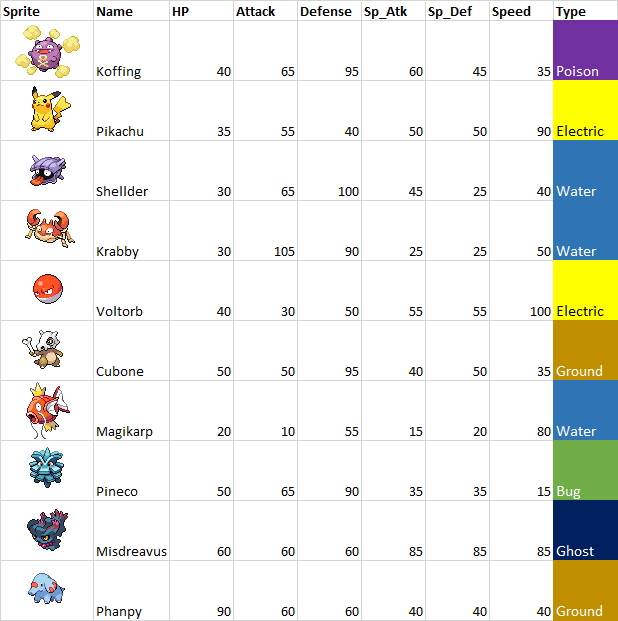
\includegraphics[width=1\linewidth]{figuras/pokemon_cate.png}
  \caption{Categorical representation of Pokémon types.}
  \label{fig:pokecat}
\end{subfigure}
\begin{subfigure}{.7\textwidth}
  \centering
  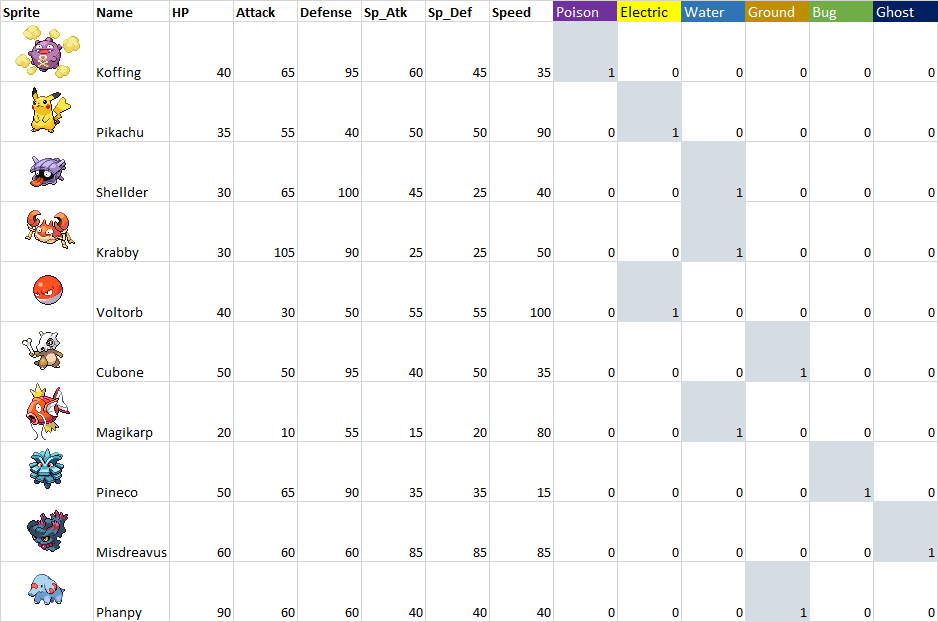
\includegraphics[width=1\linewidth]{figuras/pokemon1hot.png}
  \caption{One-hot encoding of Pokémon types.}
  \label{fig:pokehot}
\end{subfigure}
\caption{Table of a few Pokémon statistics representing its type as a \textbf{(a)} categorical variable or as an \textbf{(b)} one-hot encoding. In this case, the Pokémon types of a trainer could be represented by a bag-of-words by adding the one-hot encodings\footnote{Albeit it would be more of a ``bag-of-types'' than a bag-of-words}. Base stats from Generation VI from \citet{bulbapedia} and images from \citet{hotpokemon}.}
\label{fig:poke}
\end{figure}




However, these approaches are inefficient. Vocabularies tend to be huge, Merriam-Webster's Third New International Dictionary \citep{merriam} possesses $470,000$ different entries, but a typical sentence would not be longer than $100$ words. This leads to a sparse representation of sentences and also loses important information such as the order of appearance of the words in the sentence.

Embeddings are an efficient approach to solve these problems; an embedding is a low-dimensional space (in comparison to the huge size of typical vocabularies) into which one can translate high-dimensional vectors. In essence, an embedding tries to project into a lower dimensional space high-dimensional vectors in such a way that the ones that are ``similar'' are closer in the embedding space. In the case of words, we are interested in the semantic similarity between them but they may be similar in unexpected ways, depending on the training method antonyms may be closer than synonyms because they are used in similar ways.

Embeddings are not exclusive to natural language processing, they are used to deal with the sparsity of adjacency graphs, in graph neural networks, to permit the use of graphs as input for more conventional NNs \citep{grover2016node2vec} and may even be used with any machine learning model that deals with too many features, being particularly useful with boolean and categorical variables. They are also not exclusively used with individual words, they may be used with entire sentences \citep{sbert_paper}, paragraphs or even entire documents at once \citep{doc2vec}.


Another benefit of embeddings is that they have high re-usability, it is not uncommon to re-utilize them across different models and tasks. To further improve their performance there are many transfer learning techniques that can be leveraged, but depending on the application they may not even need fine tuning to achieve an acceptable performance.


We will now present an overview of an embedding called \textit{word2vec} to better illustrate embeddings and their uses.




\subsection{Word2vec}

Word2vec \citep{word2vec_original} is an algorithm that produces word embeddings. A word embedding as previously mentioned is a mapping of words into a vector space $\mathbb{R}^{n}$, i.e. each word can be represented as a vector of real numbers. 
The power of these embeddings created by word2vec comes from its dense distributed representation, wherein $\mathbb{R}^{n}$  is such that $n$ is smaller than the number of distinct words in the corpus and is capable of capturing some of the underlying syntactic and semantic structure of the language.

As an example of this structure we can take the vector representation for the words $king$, $queen$, $man$ and $woman$ and calculate  $king - man + woman$. This will provide us a new vector that is closer to $queen$ then any other word vector, as can be seen in the illustration of Fig.~\ref{queen}. In Figure~\ref{figur_word2vec} we can see other examples of such relationships captured by word2vec.





\begin{figure}[!ht]
\centerline{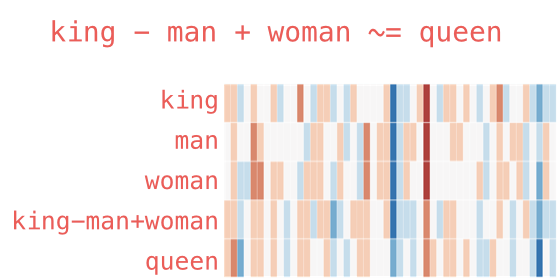
\includegraphics[width=0.8\textwidth]{figuras/queen.png}}
\caption{The resulting vector from ``king-man+woman'' doesn't exactly equal ``queen'', but ``queen'' is the closest word to it from the 400,000 word embeddings in this collection. Color coded cells based on their values (red if they’re close to 2, white if they’re close to 0, blue if they’re close to -2). \citep{jallamarword2vec}}
\label{queen}
\end{figure}




\begin{figure}[!ht]
\centerline{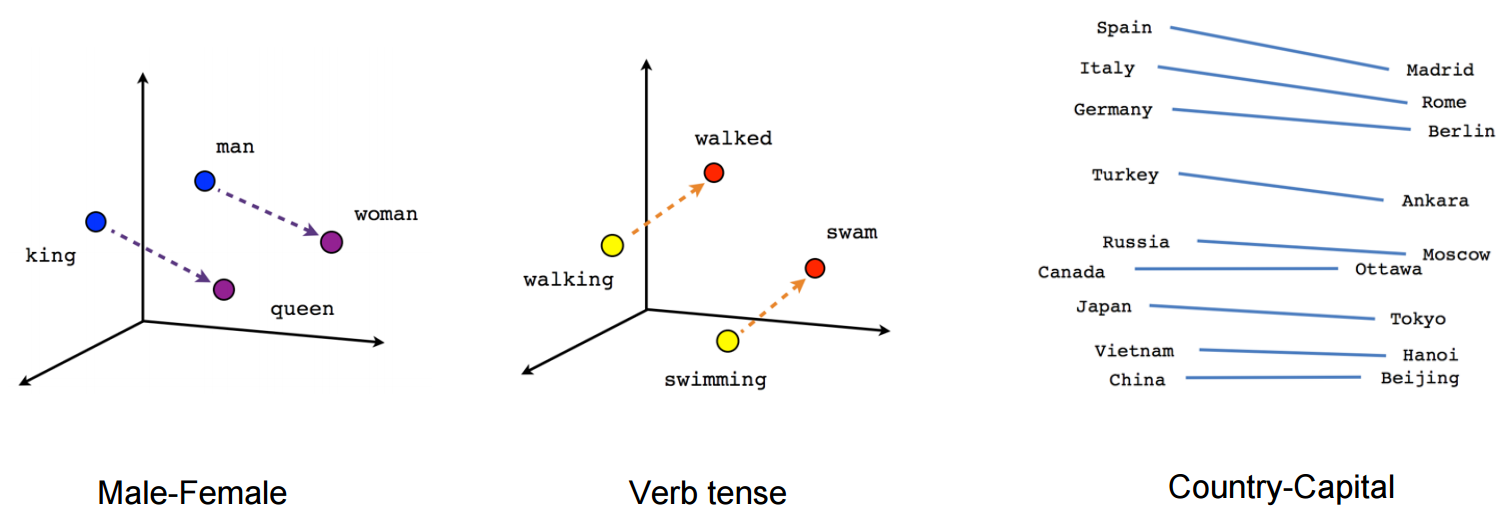
\includegraphics[scale=0.25]{ilustracao_word2vec}}
\caption{Illustration of some semantic and syntactic relations captured by word2vec embeddings, vectors whose words have similar relationships (such as gender or conjugation) tend to also have similar relations on the vector space \citep{ilustracao_word2vec}. This is nothing more than an illustration since usual embeddings are of such a high order that visualization as a simple 3D plot becomes impossible, dimensionality reduction techniques (e.g. PCA) albeit useful may lead to spurious relations, when searching for such relations it is customary to use appropriate distance metrics such as the cosine distance.}
\label{figur_word2vec}
\end{figure}

These relationships are obtained during its training process, at first each word is assigned a word embedding composed of purely random numbers that will converge into a meaningful embedding. The training process of this algorithm is based on the idea that one may deduce the meaning of a word by its context, so by updating the embedding of a word by using the embedding of its neighbors or vice-versa it is possible to capture semantic and syntactic information from the language thus construing a meaningful embedding space.

This idea of understating a word by its context is nothing new going at least as far as 1957:

\begin{myquote}
\textit{You shall know a word by the company it keeps.}\\
\citet{firth1957synopsis}
\end{myquote}

Word2vec was one of the first models to efficiently utilize this idea, being quickly followed by GloVe \citep{glove}, a model that leverages the co-ocurrence matrix of words to train its embedding, and many others. An example of a co-ocurrence matrix can be seen in Fig.~\ref{coocurence}. Even though nowadays there are many embeddings more powerful than those two, they are still useful for simpler applications as tried and tested methods or even because of their relatively high computational efficiency.


\begin{figure}[!ht]
\centerline{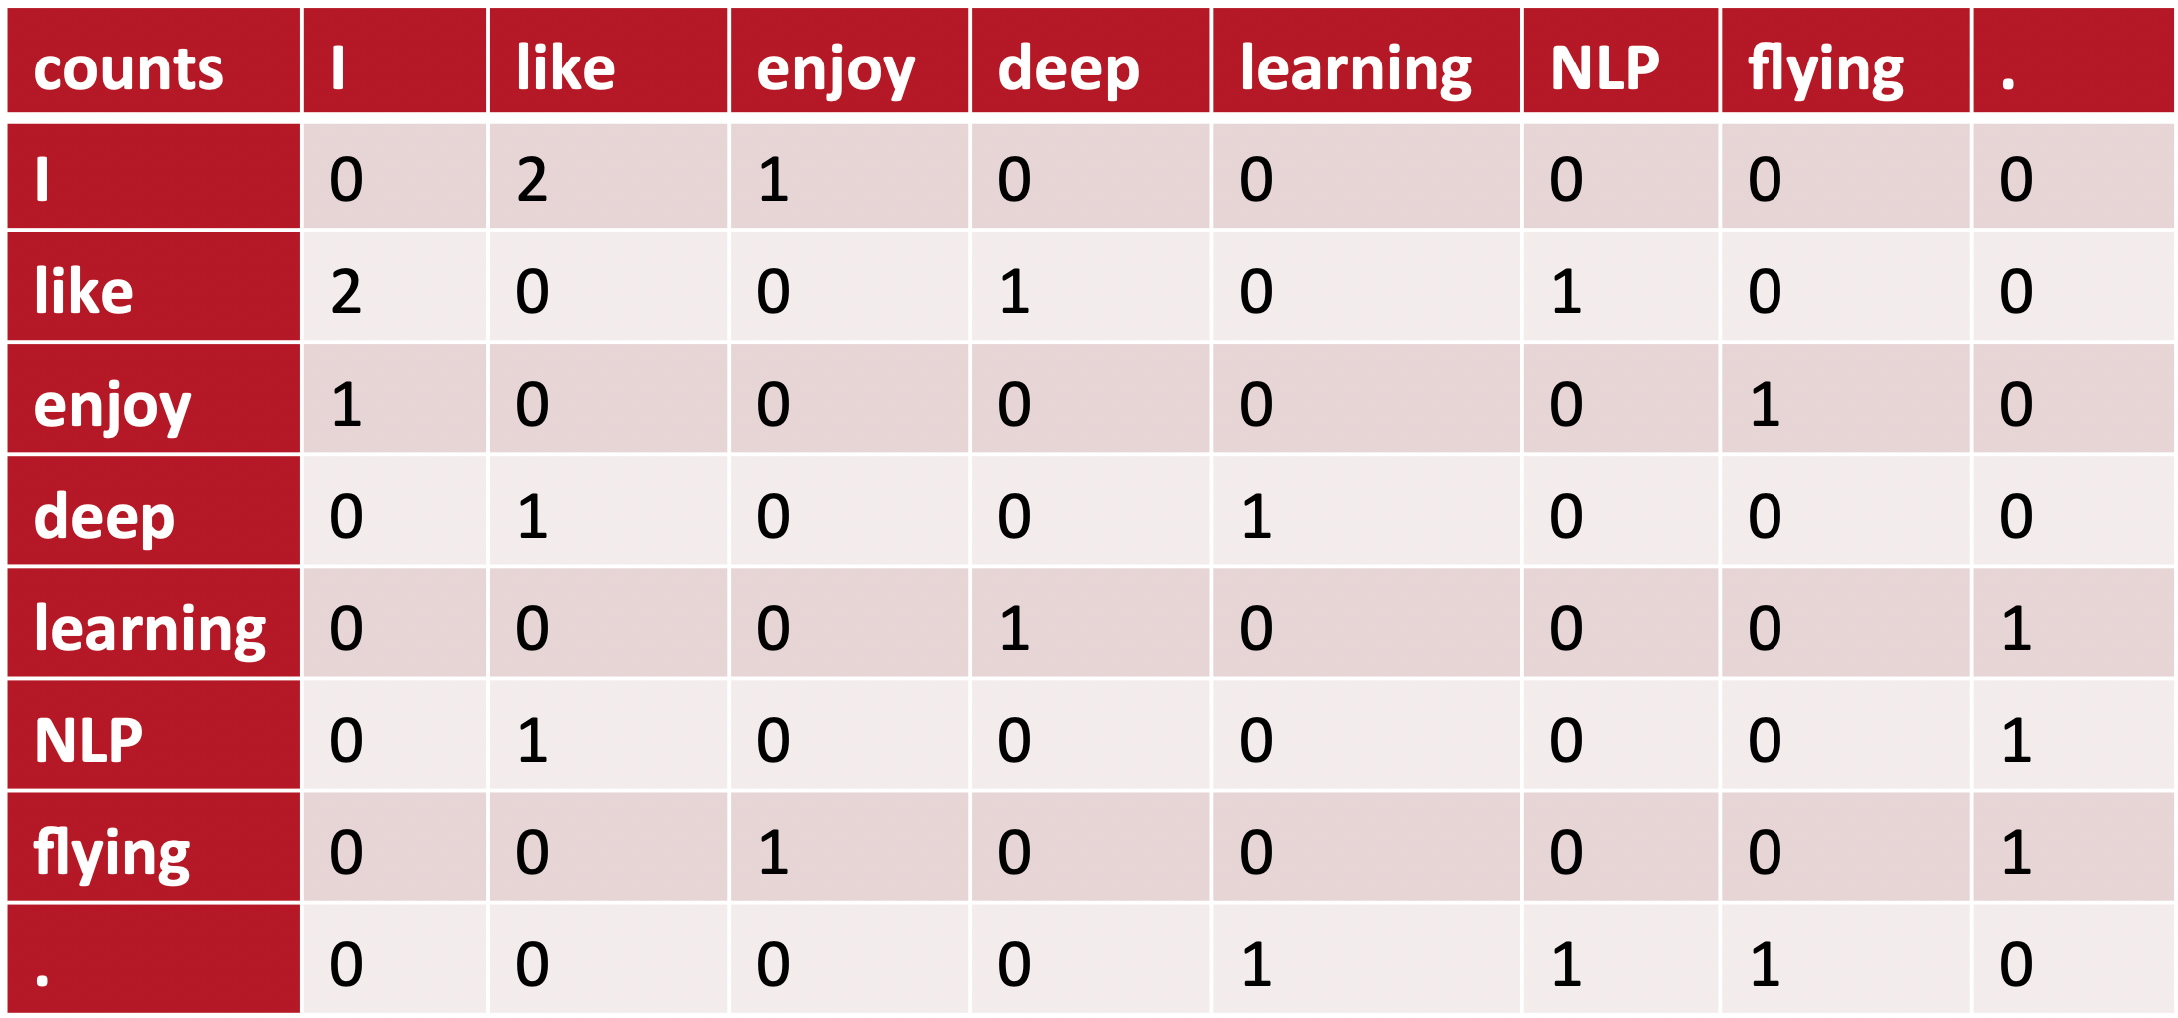
\includegraphics[width=0.85\textwidth]{figuras/coocurence.png}}
\caption{Example of a co-ocurrence matrix with a symmetrical window of size 1.\\
Corpus: I like deep learning. I like NLP. I enjoy flying.\\
Dictionary: [ 'I', 'like', 'enjoy', 'deep', 'learning', 'NLP', 'flying', '.' ] \citep{coocurrence}
}
\label{coocurence}
\end{figure}

\section{LSTM}

\begin{figure}[!ht]
\centerline{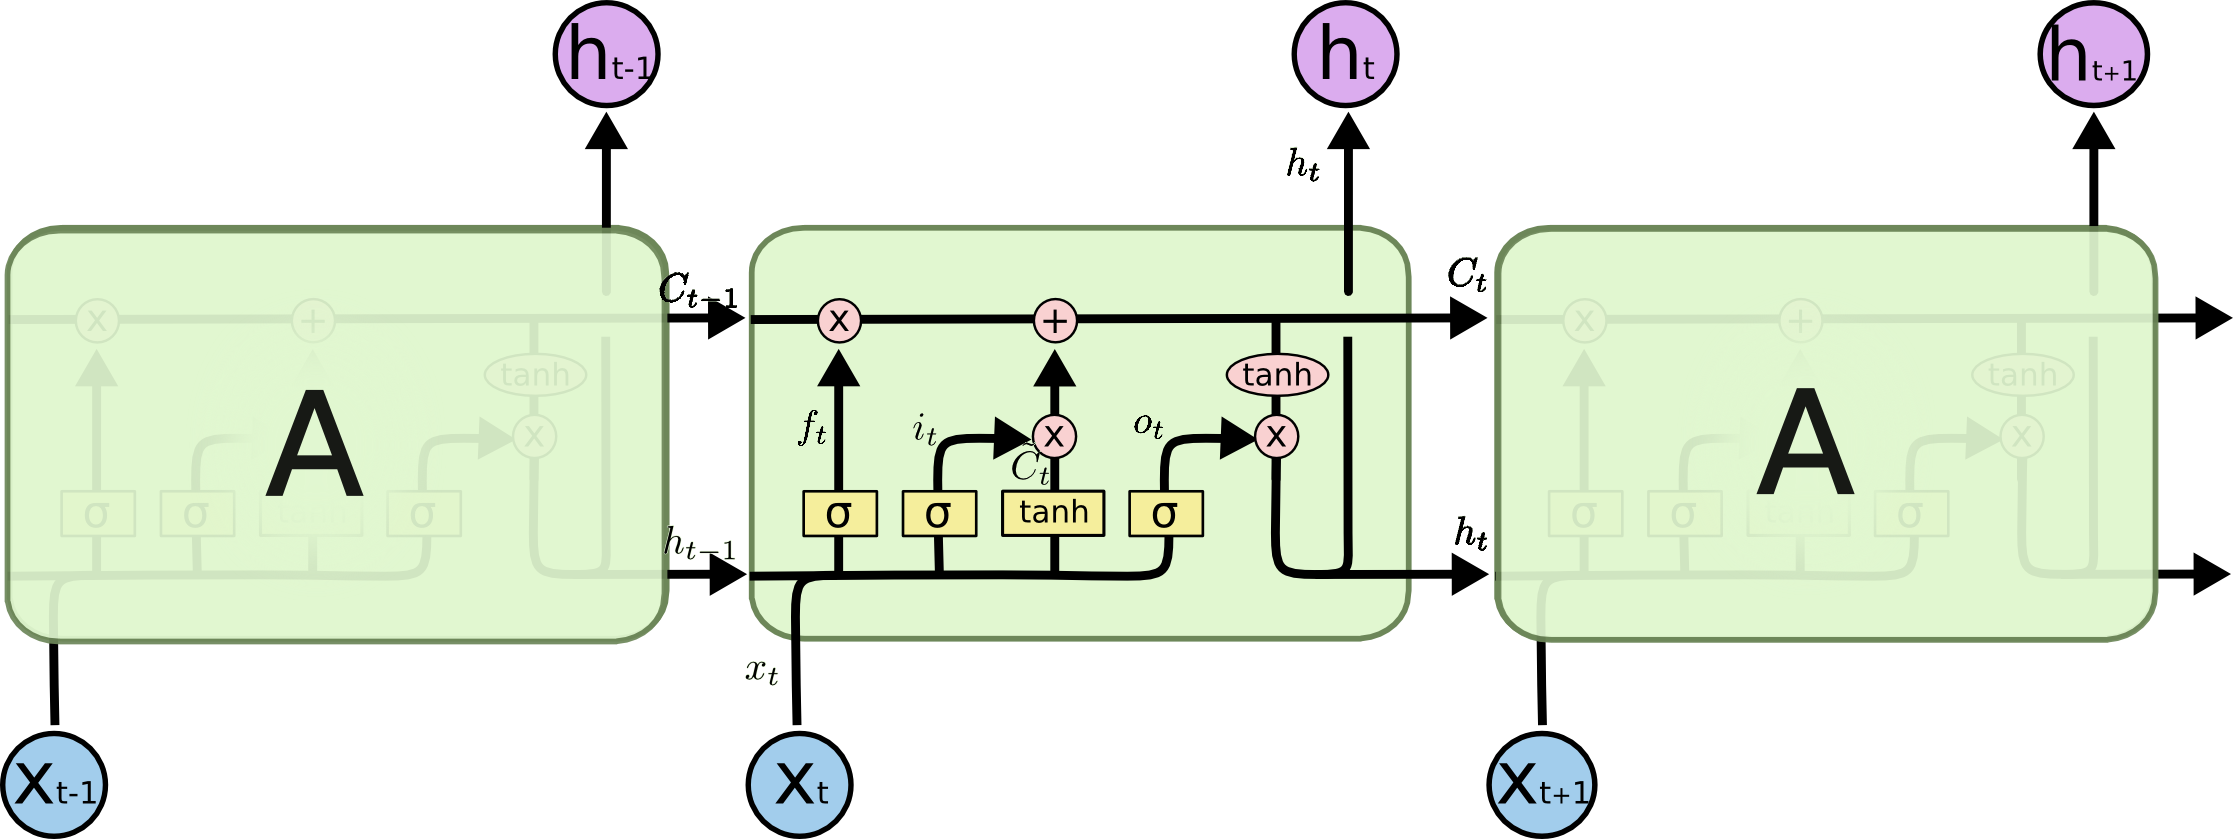
\includegraphics[width=1.1\textwidth]{figuras/lstm.png}}
\caption{An illustration of the LSTM architecture, image adapted from \citet{lstm_imagem}.
}
\label{fig:lstm}
\end{figure}

LSTM, or Long Short-Term Memory \citep{lstm}, is a recurrent neural network architecture developed to tackle the problem of vanishing gradient when dealing with long inputs in RNNs where the ``gradient flow'' would vanish, resulting in stagnation during training and the inability to deal with long distance relationships in, for example, long sentences or paragraphs. This inability to go beyond ``short-term memory'', was improved by introducing a better information flow in the network, giving it the ability to learn when to ``forget'' and when to ``update'' accordingly.
An illustration of this architecture can be seen in Fig.~\ref{fig:lstm}, but it can be described by its three gates:

\begin{itemize}
    \item[] Forget gate:  $f_t = \sigma(W_f . [h_{t-1},x_t] + b_f)$
    \item[] Input gate: $i_t = \sigma(W_i . [h_{t-1},x_t] + b_i)$
    \item[] Output gate: $o_t = \sigma(W_o . [h_{t-1},x_t] + b_o)$ 
\end{itemize}

The forget gate is responsible for ``deciding'' what to keep from earlier steps, the input gate for what to keep from the current step and the output gate for the next hidden state $h_t$. Another integral part of this model is the cell state $C_t$ and the \textit{candidate} cell state $\tilde{C}_t$, responsible for ``storing'' the information on the network, being updated at each time step based on the candidate cell state, the input gate and the forget gate:


\begin{itemize}
    \item[] $\tilde{C}_t = \textit{tanh}(W_C . [h_{t-1}, x_t] + b_C)$
    \item[] $C_t = f_t * C_{t-1} + i_t * \tilde{C}_t$ 
    \item[] $h_t = o_t * \textit{tanh}(C_t)$
\end{itemize}


\section{Encoder-Decoder}
The idea behind the encoder-decoder neural network architecture is to use an encoding layer to create an intermediary representation of the input that will subsequently be transformed by the decoder layer into the desired target.
Recurrent neural networks such as LSTMs or GRUs \citep{GRU} are commonly used as the encoding and decoding layers to avoid the vanishing gradient problem. %, they are able to do so by using feedback loops to obtain information persistency.
 A common use of the encoder-decoder architecture is machine translation through seq2seq \citep{seq2seq}. For example, an english text can be used as an input to the encoder which will generate a latent space vector, an abstract representation of the text, that will be used by the decoder to generate a french translation of the original text. This process can be visualized in Fig.~\ref{contextvec}.

\begin{figure}[!ht]
\centering
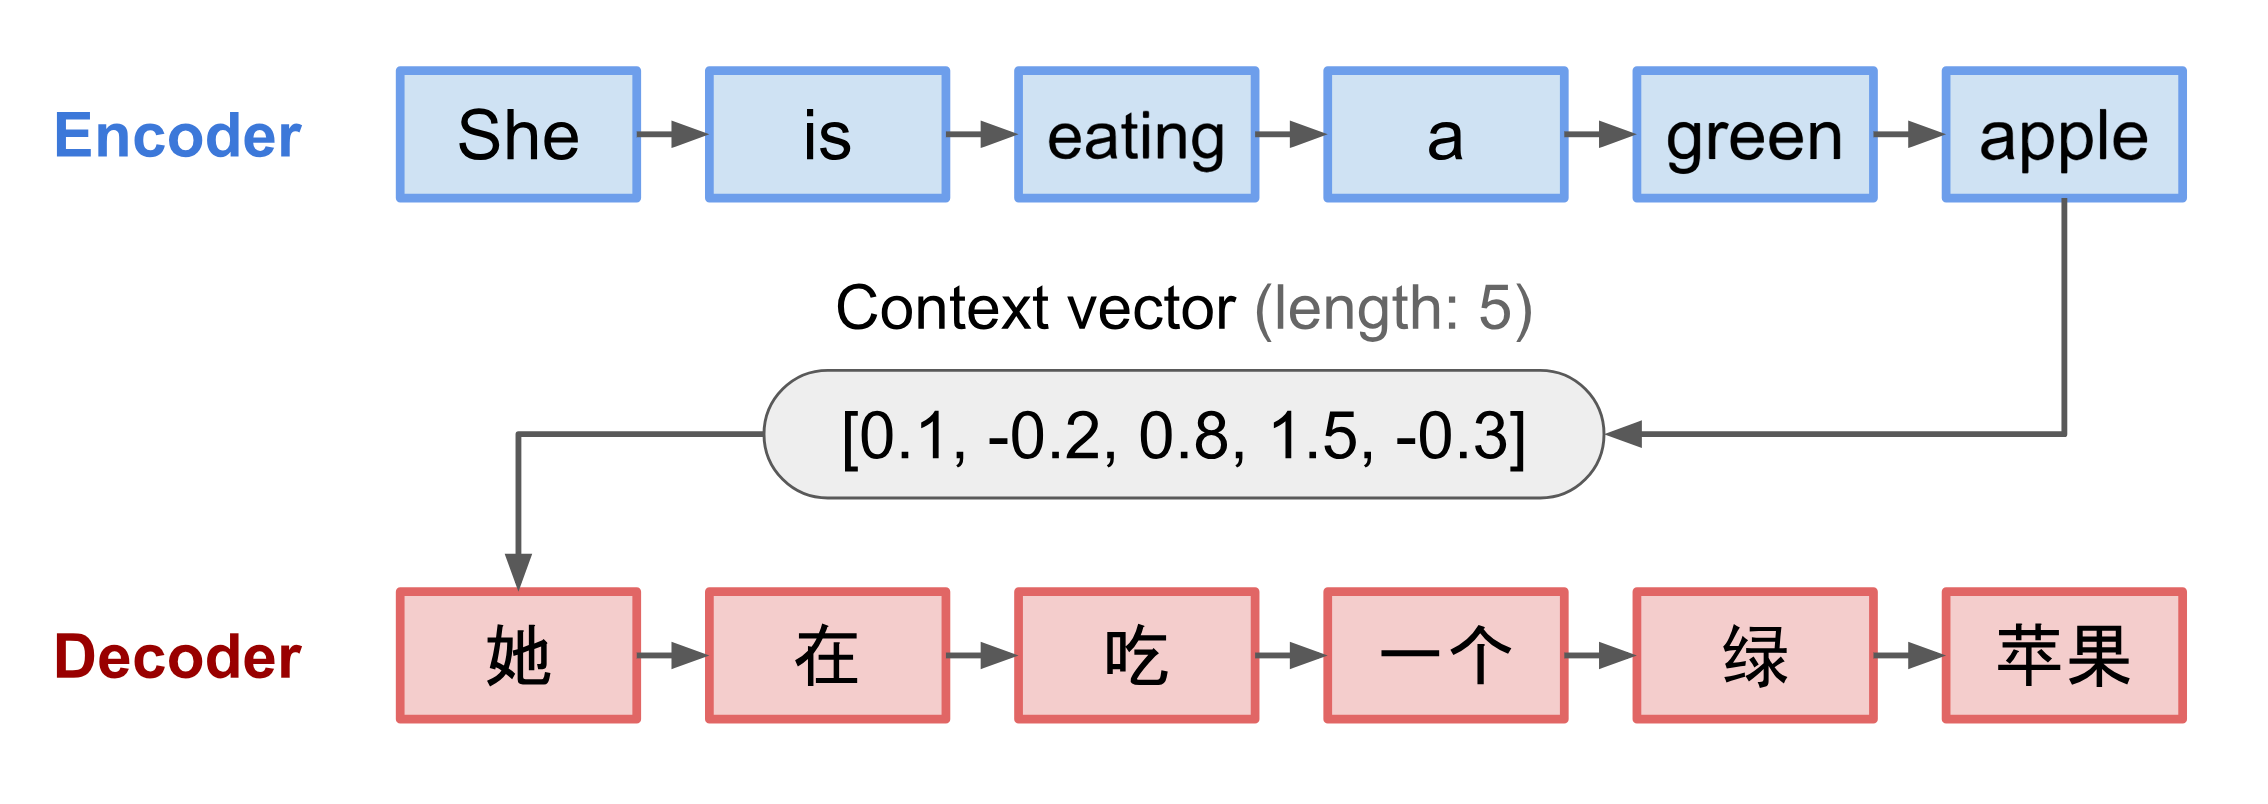
\includegraphics[width=0.9\textwidth]{figuras/context_vector.png}
\caption{\textit{The encoder-decoder model, translating the sentence ``she is eating a green apple'' to Chinese. The visualization of both encoder and decoder is unrolled in time.} \citep{weng2018attention}\\ The context vector in gray is the intermediary representation between the encoder and decoder that needs to hold all the relevant information to successfully realize the translation without referencing the original input in english. }
\label{contextvec}
\end{figure}


Another example of the encoder-decoder architecture are the autoencoders, where the objective is to make the output predict the input. The existence of an intermediate state outputted by the encoder forces the autoencoder to learn a compact representation of the input and try to reconstruct it as the output, an illustration can be seen in Fig.~\ref{autoencoder}.


\begin{figure}[!ht]
\centering
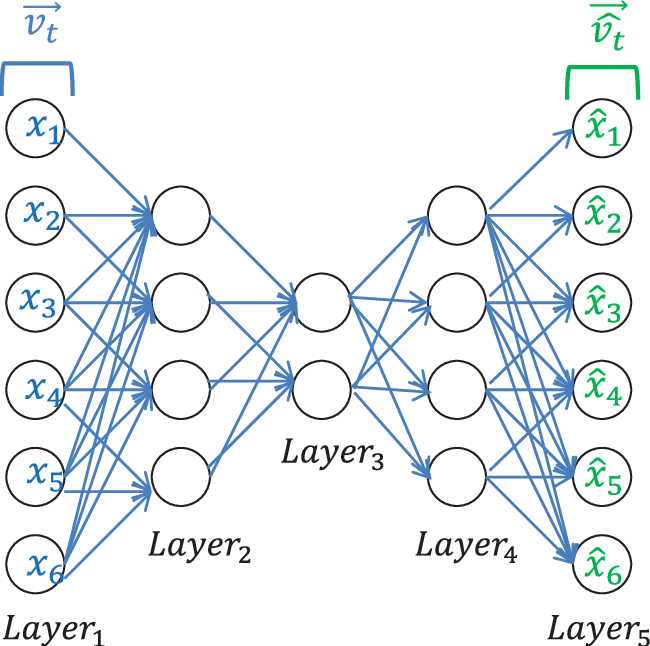
\includegraphics[scale=0.3]{An-illustration-of-AE-learner.png}
\caption{Illustration \citep{imagem_autoencoder} of a shallow autoencoder. $\vec{v}$ and $\vec{\hat{v}}$ represent the input and output respectively of the network while the output from layer 3 is responsible for the compact representation of the input on the latent space. The encoder is composed of layers 1, 2 and 3 while the decoder is composed of layers 4 and 5.}
\label{autoencoder}
\end{figure}

\section{Attention}
Attention comes to address one of the main drawbacks of the encoder-decoder architectures, the informational bottleneck. By forcing the entire sequence of information to be contained in a single vector it becomes increasingly difficult to capture long-range relations and information presented at the beginning of long input sentences. 
Attention provides a simple manner of capturing the relevant input tokens for each token of the output, generating an attention matrix that represents the relevant context for each token and improving interpretability.


\begin{figure}[!ht]
\centerline{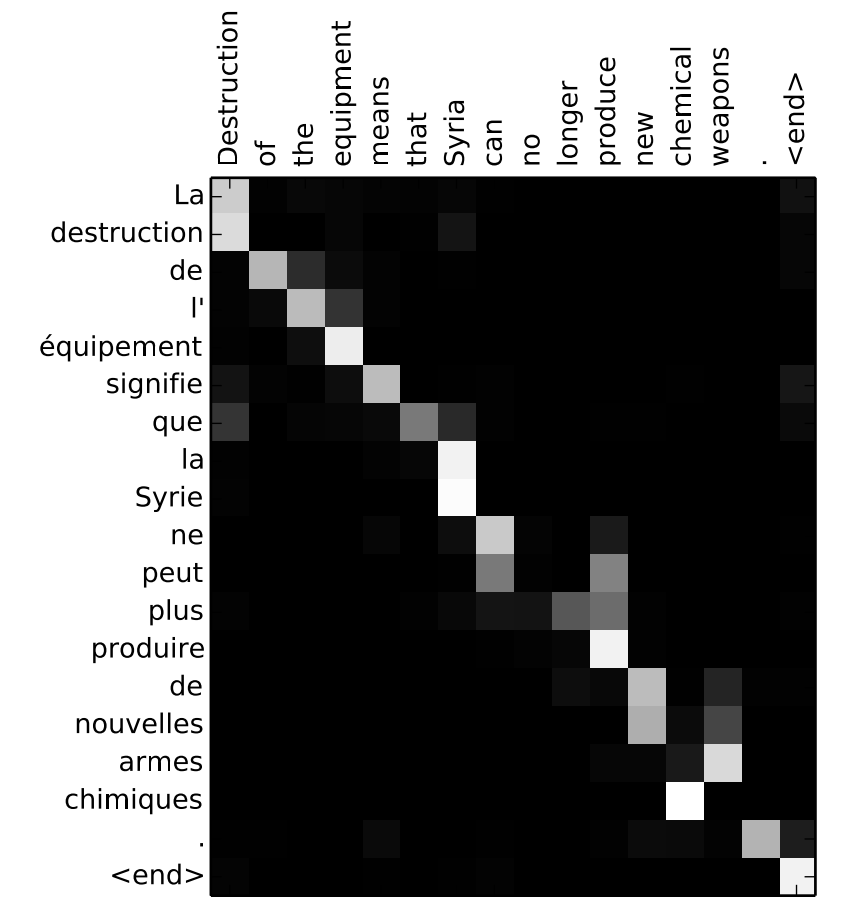
\includegraphics[scale=0.5]{attention_matrix.png}}
\caption{Illustration \citep{attention_matrix} of an example attention matrix for a sentence in english and it's french translation. }
\end{figure}

This provides another counter-measure against the vanishing gradient problem by connecting the entirety of the input to the training process, but the biggest insight of attention is this idea of paying attention to a specific part of the input that is more relevant to obtain our desired output. For example, given the obscured photo in Fig.~\ref{img:dog_escondido} how would one describe its content? We could guess about the gender, origins or facial expression of the depicted person, but we would most likely assume it depicts a human and not a dog as can be seen in Fig.~\ref{img:dog}, but how did we arrive at this conclusion? Which part of the image implies the presence of a human? This is the essence of the idea behind attention, where to look at to answer something. 





\begin{figure}
\centering
\begin{subfigure}{.45\textwidth}
  \centering
  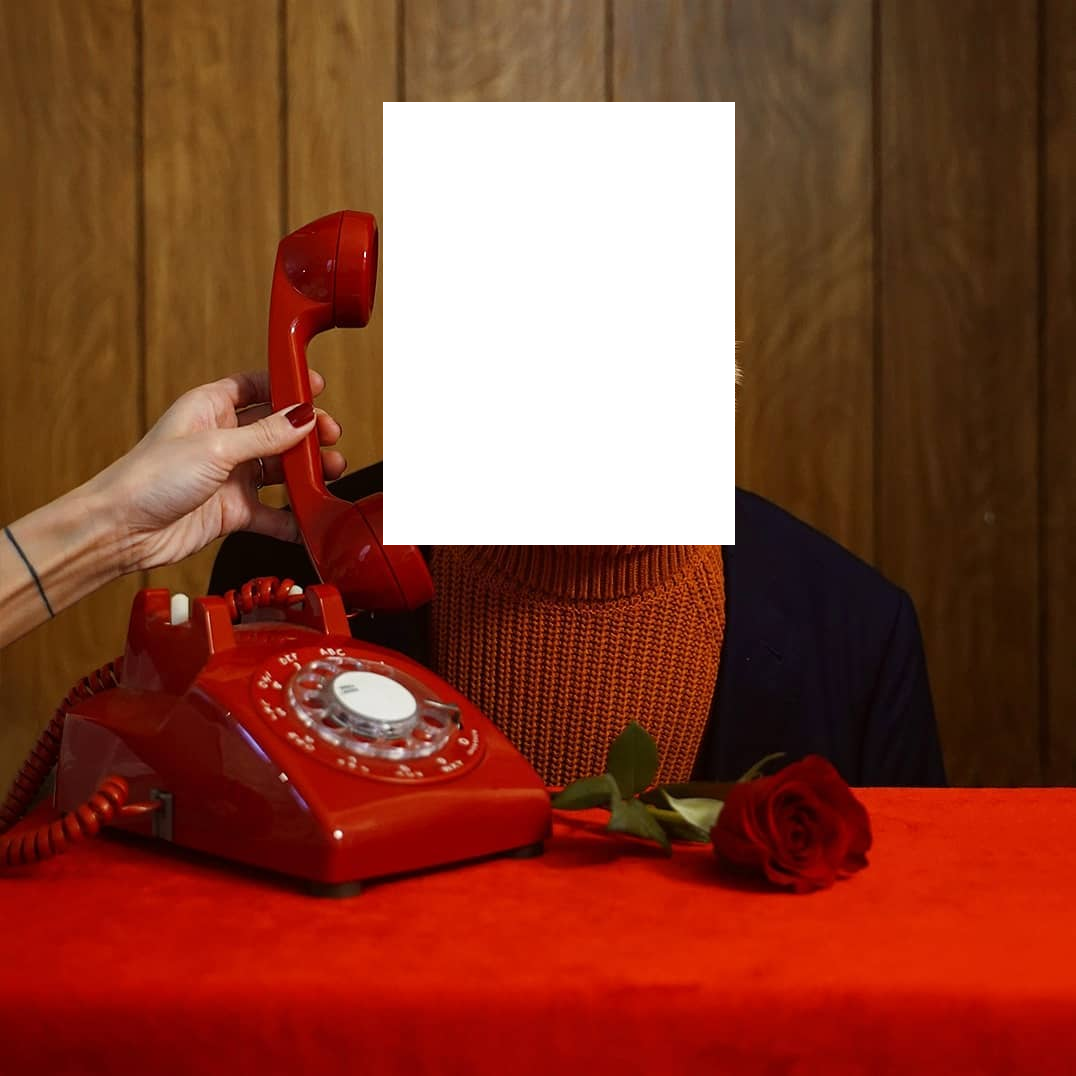
\includegraphics[width=1\linewidth]{figuras/dog_obscuro.png}
  \caption{}
  \label{img:dog_escondido}
\end{subfigure}
\begin{subfigure}{.45\textwidth}
  \centering
  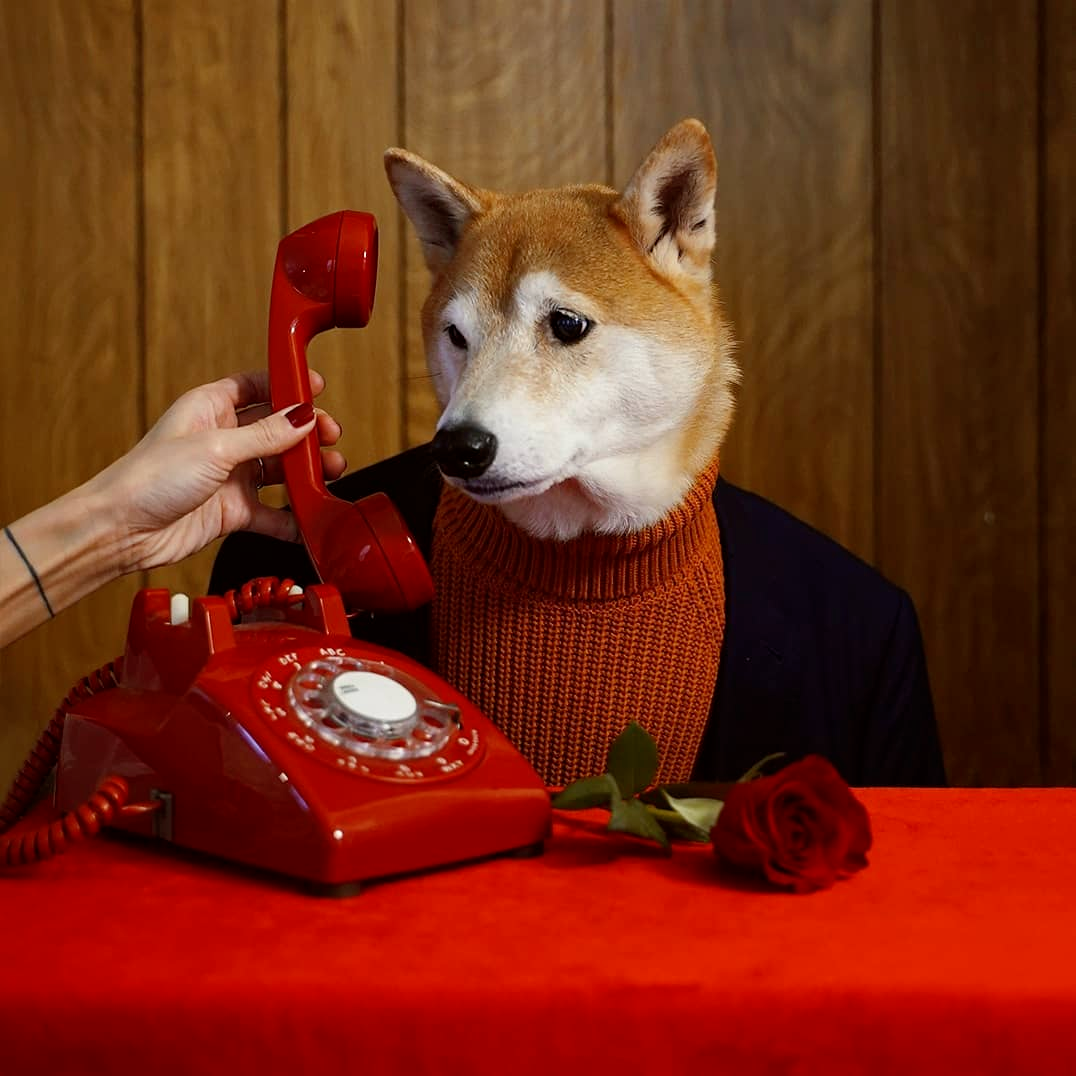
\includegraphics[width=1\linewidth]{figuras/dog.png}
  \caption{}
  \label{img:dog}
\end{subfigure}
\caption{A collage to illustrate the idea of attention and visual attention. Photo obtained from \citet{dog}.}
\end{figure}



\citet{atencao_review} generalized attention by breaking it into three swappable components: the 3-tuple (key, query, value), the score function and the distribution function. 
% Since many new types of attention were being continuously developed, a framework to generalize them was, and still is, necessary to better understand and differentiate them. If this particular nomenclature will take root on the machine learning community or not only time can tell, but we will be adopting it in this work nevertheless.


The tuple (key, query, value) are the input for the score function, the objects upon which we desire to calculate the attention. The score function is used to calculate the energy scores that will be subsequently passed through the distribution function to produce the attention scores such as the \textit{softmax} function that also normalizes the scores into a probability distribution.

Fig.~\ref{fig:atencao_geral} illustrates this general framework and Fig.~\ref{img:luong} gives an illustrative example of one of the first attention implementations.

  
\begin{figure}[!ht]
\centering
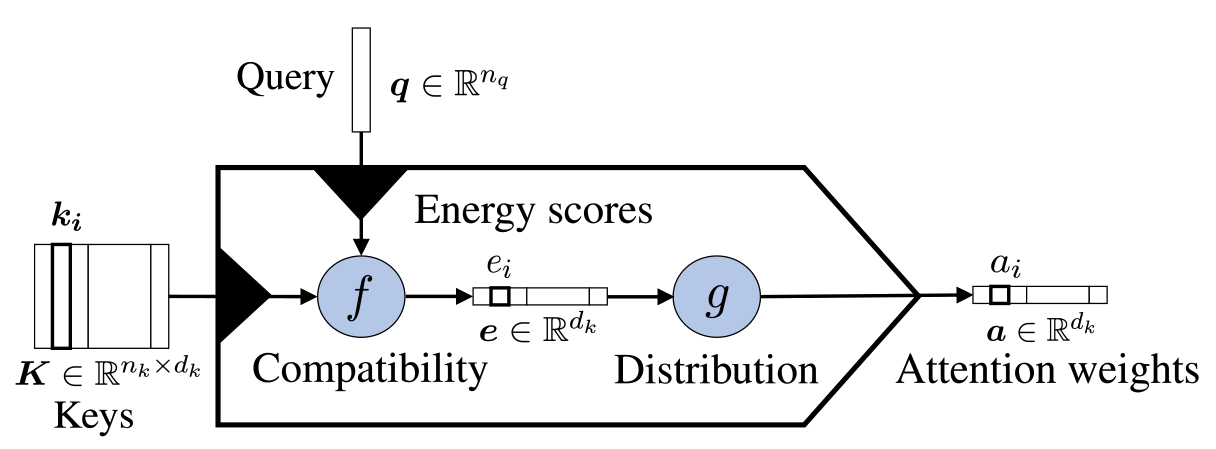
\includegraphics[width=0.8\linewidth]{figuras/atencao_geral.png}
\caption{Illustration of \citet{atencao_review} general attention framework. The ``Value'' component is not present in this illustration but could be used in a subsequent step to process the attention scores to create a context vector. }
\label{fig:atencao_geral}
\end{figure}


\begin{figure}
\centering
\begin{subfigure}{.5\textwidth}
  \centering
  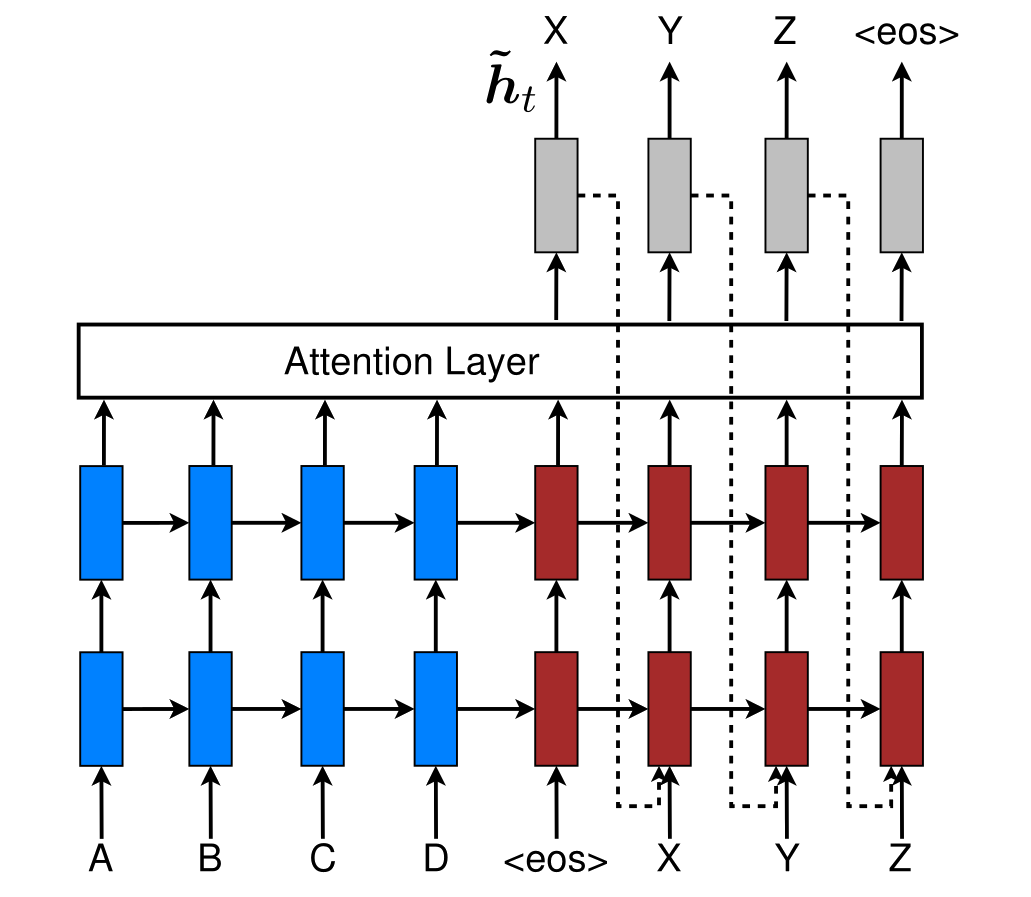
\includegraphics[width=1\linewidth]{figuras/luong1.png}
  \caption{Illustration of an encoder decoder model with attention, every decoder step decides the next token based on the context vector and the last decoder hidden state. The blue rectangles represent the encoder and the red ones the decoder.}
  \label{img:luong1}
\end{subfigure}
\begin{subfigure}{.75\textwidth}
  \centering
  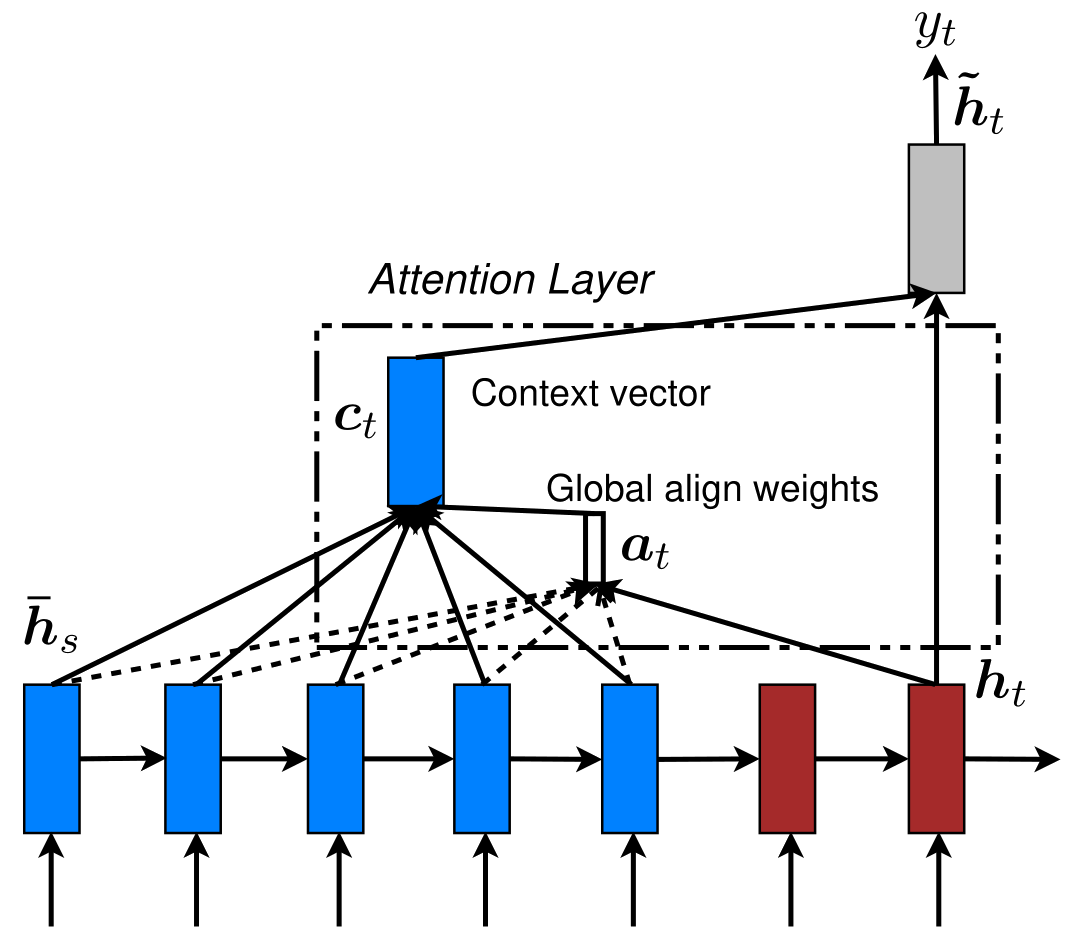
\includegraphics[width=1\linewidth]{figuras/luong2.png}
  \caption{To calculate the attention all encoder hidden states $\bar{h_s}$ (Keys)\footnote{In this case Key and Value are the same} and the current decoder hidden state $h_t$ (Query) are passed to the score function $score(h_t, \bar{h}_s) = h_t^\top \bar{h}_s$ to calculate the energy scores. Then the energy scores are passed to the distribution function softmax $a_t(s)= \frac{exp(score(h_t, \bar{h}_{s}))}{\sum_{{{s}}'} exp(score(h_t, \bar{h}_{{s}'}))}$ to generate the attention score.
    How to use an attention score may vary between architectures and applications, in this particular case \citet{luong2015effective} takes the weighted average $c_t =\frac{\sum_s \bar{h}_i a_i}{|s|}$ of all attention scores to create a context vector which will be used with the decoder hidden state to predict the next word.
}
  \label{img:luong2}
\end{subfigure}
\caption{Fig.~\ref{img:luong1} illustrates an encoder decoder model and Fig.~\ref{img:luong2} illustrate its attention mechanism, both images extracted from \citet{luong2015effective}.}
  \label{img:luong}

\end{figure}






\section{Pointer Networks}
\label{sec:ptrnet}
Pointer Net \citep{pointer}, or Ptr-Net, is a neural architecture that learns the conditional probability of an output sequence composed of index positions of the input sequence. It is essentially an encoder-decoder architecture with attention, but the attention mechanism is used at each step to determine an index of the input. Fig~\ref{ptr_hull} illustrates the difference from a normal encoder-decoder.


\begin{figure}[!ht]
\centering
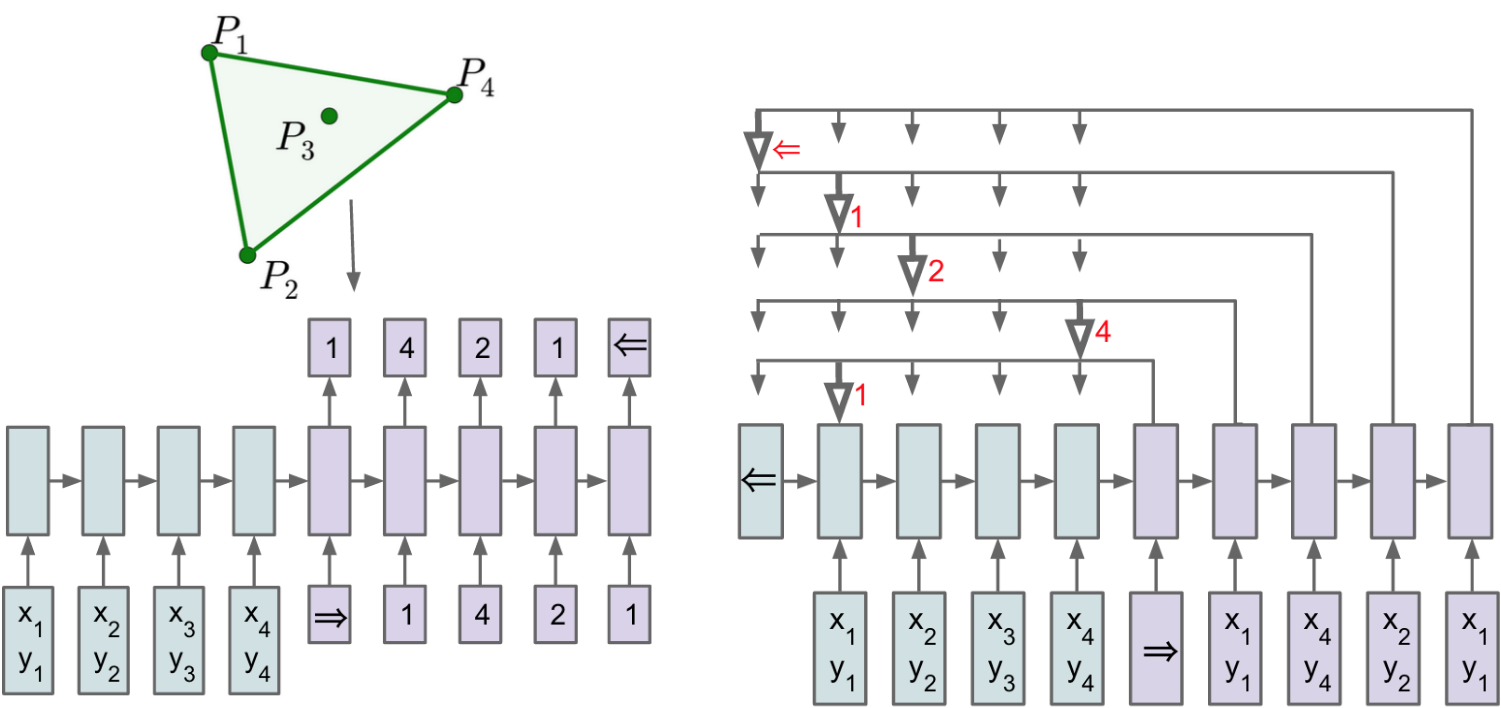
\includegraphics[scale=1.2]{figuras/ptrjunto.png}
\caption{This illustration represents 2 different architectures used to find the convex hull of a set of points \citep{pointer}. The left one is a normal encoder-decoder while on the right we have a Ptr-Net. } 
\label{ptr_hull}
\end{figure}

The original paper explores the use of this architecture with geometric problems, such as finding the convex hull as can be seen in Fig~\ref{ptr_hull}, but it can also be used for other problems. Another use of Ptr-Nets are in Q\&A tasks such as in the SQuAD dataset \citep{squad1} where a question is provided paired with a text that contains the answer to this question. A common approach \citep{squad_pointer} to answer the question is to train a model that finds in the provided text an initial and a final token that together delimit a minimal portion of the text that contains the answer. An example of such a Q\&A task can be seen on Fig.~\ref{squad}.

  
\begin{figure}[!ht]
\centering
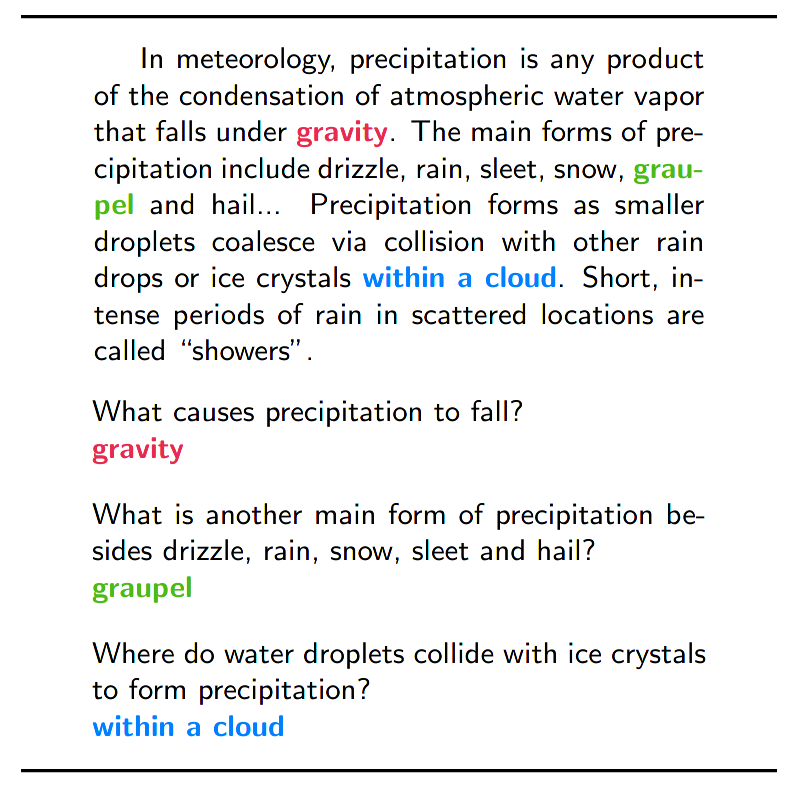
\includegraphics[scale=0.3]{squad.png}
\caption{This excerpt illustrates 3 different questions for a single paragraph of text, for the first two questions the initial and final tokens overlap as the answer is composed of a single word. On the third question the initial token would be the word ``within'' and the final token would be ``cloud'' and the resulting answer delimited by them would be ``within a cloud''. Example extracted from \citep{squad1}.}
\label{squad}
\end{figure}




\section{Transformer}
The transformer \citep{attention_is_all_you_need} is another encoder-decoder architecture but with a major difference: it shifts from the use of recurrent neural networks in favor of attention. More precisely, the encoder uses word vectors as input and is composed of a self-attention layer followed by a feed forward network.
Self-attention is capable of capturing strong semantic information, for example in the sentence ``Marie bought a cookie and ate it.'' the self-attention model is capable of determining that the token ``it'' refers to the token ``cookie''.


The transformer starts by using self-attention on the word embeddings to aggregate information from each token, creating a new context-rich representation for each word simultaneously. The decoder on the other hand takes an iterative approach, instead of outputting the entire translated sentence at the same time it generates one word at a time. The decoder utilizes the final representation output by the encoder and every word it already output to generate the next word until it predicts and $<END>$ tag. In essence it will receive the sentence to be translated as input and will output the translated sentence one word at a time. Figs.~\ref{trans_arq} and \ref{self-att} illustrate the architecture of the transformer model and the self attention mechanism.

\begin{figure}[!ht]
\centering
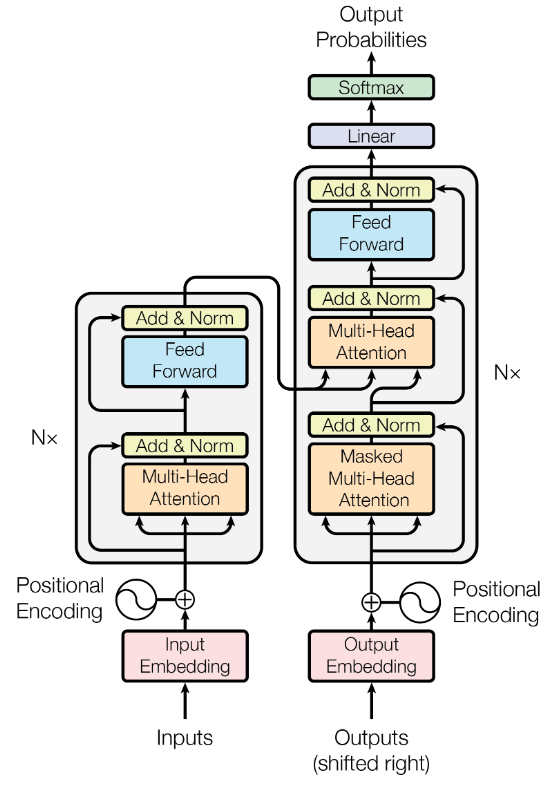
\includegraphics[scale=0.6]{figuras/transformer_arquitetura.png}
\caption{The Transformer - model architecture. \citep{attention_is_all_you_need}}
\label{trans_arq}
\end{figure}


\begin{figure}[!ht]
\centering
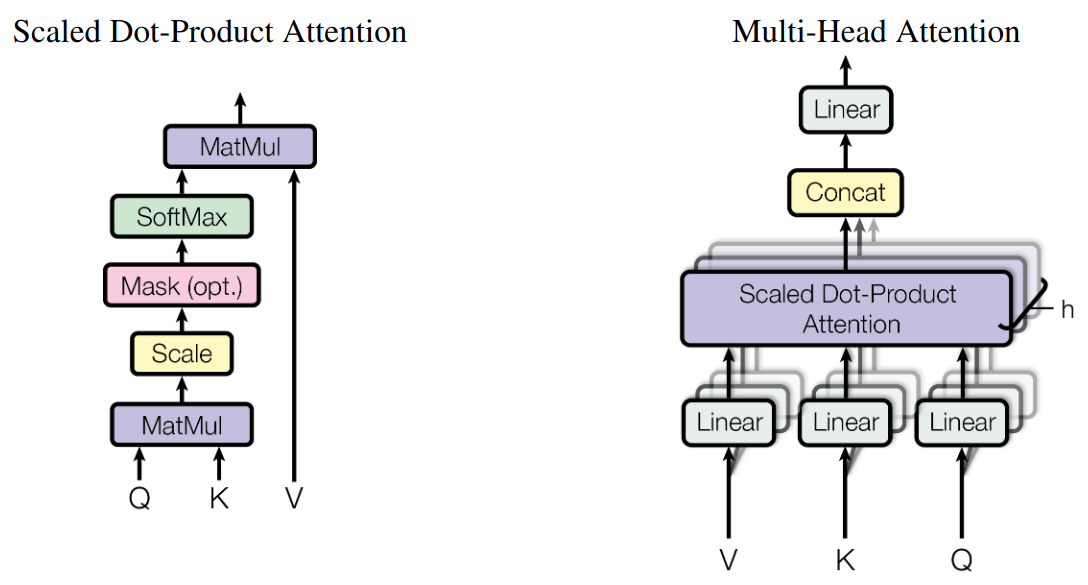
\includegraphics[width=0.9\textwidth]{figuras/self-att.png}
\caption{(left) Scaled Dot-Product Attention. (right) Multi-Head Attention consists of several
attention layers running in parallel. \citep{attention_is_all_you_need}}
\label{self-att}
\end{figure}

The transformer architecture achieved state of the art performance in translation tasks and, due to its focus in attention, it was able to be trained significantly faster than other models centered around recurrent or convolutional layers. This led to a series of new models based on the transformer architecture and the idea that attention is all you need,  one of its variants, a masked-language model composed of stacked Transformer encoders called BERT \citep{BERT}, quickly became the new baseline for NLP tasks such as \citep{rogers-etal-2020-primer}, including classification tasks.

The BERT model is capable of considering the context of a word occurrence, differently than the previously mentioned context-free embeddings word2vec an GloVe. For example, the vector for ``running'' would have different embeddings in BERT for the phrases ``He is running the company into the ground.'' and ``He is running away'' while word2vec would produce the exact same embedding.




\section{Typical seq2seq Metrics}
~\label{sec:bleu}


BLEU \citep{bleu}, or \underline{b}i\underline{l}ingual \underline{e}valuation \underline{u}nderstudy, is a corpus wide NLP metric frequently used for sequence to sequence tasks such as machine translation or text summarization. This metric is a normalized score for \textit{n}-grams overlap between the output and reference outputs (e.g. reference translations in a machine translation task) with a brevity penalty for shorter outputs.

Despite BLEU's wide spread use, it has some flaws. Among the main problems pointed out by the community are the metric's inability to take meaning and sentence structure into account, e.g. a rarer synonym could penalize a correct translation and a random shuffle of words of a correct translation could have a similar BLEU score albeit being complete nonsense \citep{bleu_shuffle}.


Another famous benchmark is the previously mentioned SQuAD 1.X \citep{squad1} and its successor SQuAD 2.0 \citep{squad2}, these are reading comprehension datasets that consist of questions posed by crowdworkers on a set of Wikipedia articles. The answers may or may not be contained in the corresponding reading passage upon which the question is theoretically posed, SQuAD 2.0 being composed of the questions from SQuAD 1.1 and 50,000 unanswerable ones written to look similar to answerable questions.

%!TeX root=../tese.tex
%("dica" para o editor de texto: este arquivo é parte de um documento maior)
% para saber mais: https://tex.stackexchange.com/q/78101

\chapter{Automated Refactoring}
\label{chap:related_work}




The ``code processing community''\footnote{There does not seem to be a consensus for a name for the area, some common names are big code and programming language processing.} may be comparatively small to the NLP community, but it is not by any means non-existent. This chapter will present related work to our goal of automating function extractions, our objective is to situate the reader about recent relevant developments and to explicitate how this project differs from recent and current works in the area.



\section{Rename Method}
The rename method refactoring is one of the most commonly performed refactorings \citep{mauricio_paper}, an illustration of it can be seen in Fig.~\ref{fig:rename_method}. Due to it essentially being an act of naming something for humans to read, it is a task that can be greatly benefited from natural language processing techniques and insights. 


\begin{figure}[!ht]
\centerline{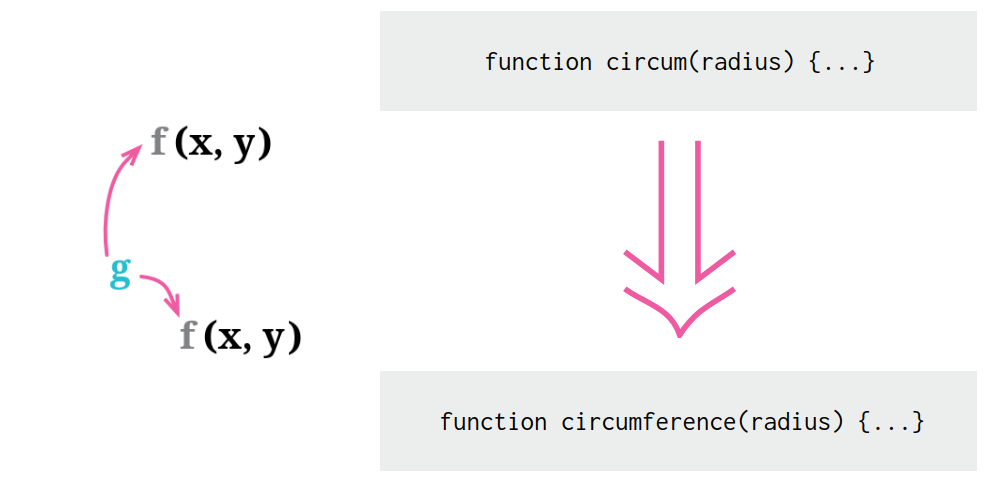
\includegraphics[width=0.6\textwidth]{figuras/rename_method.png}}
\caption{Illustration of a refactoring of the \textit{Rename Method} type. Illustration adapted from \citet{rename_method}.}
\label{fig:rename_method}
\end{figure}


In this section we will explore a few recent works that attained state of the art performance in this task at the time of their publication. But since many of them utilize an AST to achieve that, we will start by explaining what an AST is.



\subsection{AST}

For source code to become an executable program it needs to be translated into a low level language capable of being run by the machine or into machine code directly. A common approach is to write a compiler that will take the source code and compile it into an executable binary that may be used any time. A compiler is composed of numerous processing steps that can be somewhat separated into 2 categories: analysis and synthesis \citet{batata}.
The analysis part pre-processes the inputted code and generates an intermediary representation of it to be used by the synthesis step. If during the analysis the code is found to be grammatically incorrect (in respect to the programming language formal grammar) or to have any other problem of lexical, syntactical or semantic nature it will abort the compilation process and report to the user an error message. By the end of a successful analysis step an intermediary representation of the source code will be generated, e. g. an Abstract Syntax Tree.


The AST is created by taking its concrete counterpart the concrete parse tree, also known as a parse tree, and removing any redundant or unnecessary information such as idiosyncrasies related to the source language or precedence and punctuation tokens (such as parenthesis in arithmetic expressions or ``;'' to denote the end of a statement) that are made unnecessary once the parse tree is built. 
Or as it is succinctly described in the book \textit{Modern Compiler Implementation in Java}:


\begin{myquote}
\textit{The abstract syntax tree conveys the phrase structure of the source program, with all parsing issues resolved but without any semantic interpretation.} \\\citet{java_tigre}
\end{myquote}


It is no surprise that ASTs are often selected as a starting point for code embeddings, as it captures the structure of the source code that is not readily available when analyzing solely the source code.
An AST can be seen in Fig.~\ref{fig:ast} and its corresponding source code in Listing~\ref{listing:hello}.




\begin{listing}[!ht]
\inputminted[linenos, breaklines]{java}{conteudo/code/hello.java}
\caption{Small Java script, its AST can be seen in Fig.~\ref{fig:ast}.}
\label{listing:hello}
\end{listing}



\begin{landscape}
\begin{figure}[!ht]
\centerline{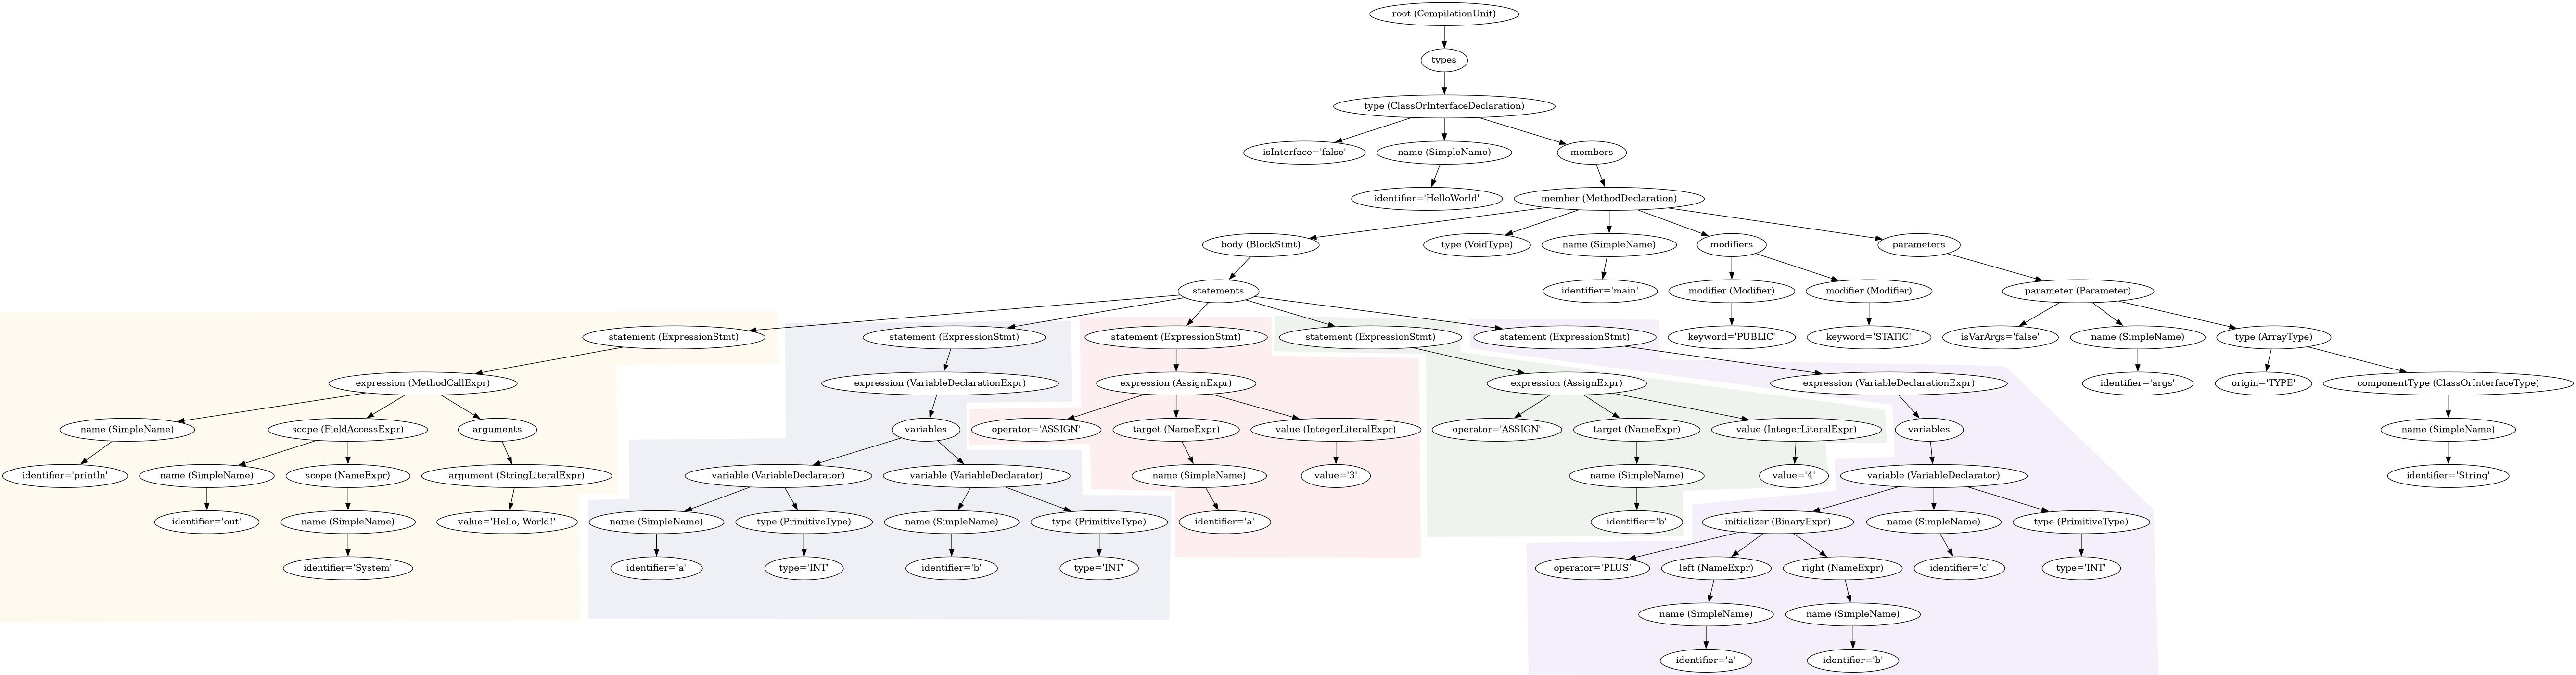
\includegraphics[height=0.5\textheight]{figuras/hello_astfinal_colorido.png}}
\caption{AST of Listing~\ref{listing:hello}. In an attempt to make the AST more intuitive and easier to read for those that never worked with them, we colored the sub-trees that correspond to the lines of the function body with one color per corresponding line\footnote{Since Java utilizes ``;'' to denote the end of a statement, multiple statements could be present in a single line of code but the AST would break down each line in its composing statements with one sub-tree for each. The existence of different lines is simply syntactic sugar, all Java programs could be expressed in single lines}. AST printed through the \texttt{dot} utility and the \texttt{JavaParser}  package, the code utilized to print the AST is available at Appendix~\ref{an:astcoisas} as Listing~\ref{listing:printer}.}
\label{fig:ast}
\end{figure}
\end{landscape}




\subsection{code2vec and code2seq}

Code2vec \citep{code2vec} is an algorithm that generates code embeddings, i.e. distributed representation of code and similar in spirit to word2vec. 
A path-based attention model was developed for learning embeddings of arbitrary-sized snippets of code, which was done through the use of paths in the program’s abstract syntax tree as a representation for code.
The authors managed to leverage the underlying structure of the programming language to develop a scalable and efficient code embedding generator.


\begin{figure}[!ht]
\centerline{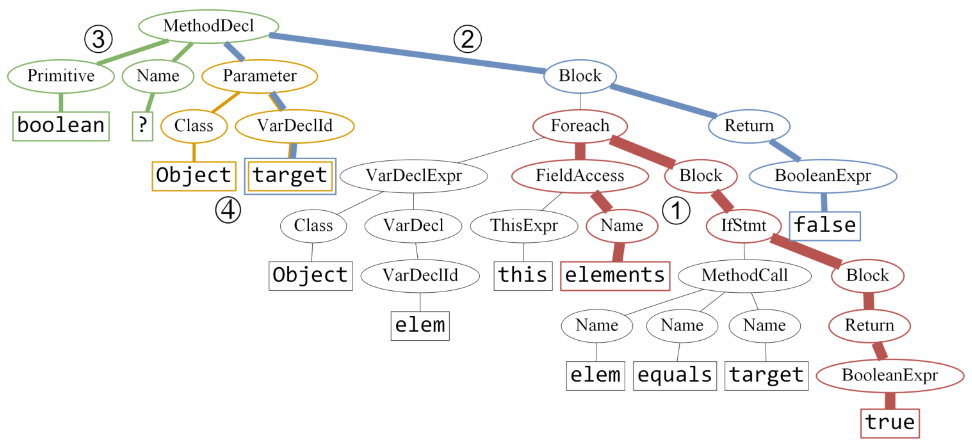
\includegraphics[width=\textwidth]{figuras/code2vecpaths.png}}
\caption{Illustration of the path-based attention model from code2vec. The width of each colored path is proportional to the attention it was given (red 1: 0.23, blue 2: 0.14, green 3: 0.09, orange 4: 0.07). \citep{code2vec}}
\label{fig:code2vec}
\end{figure}

Similarly to word2vec, this representation was successful in learning syntactic and semantic information, being able to generate analogies such as ``$receive$ is to $send$ as $download$ is to: $upload$''. 

Furthermore, code2vec was shown to be capable of capturing the resulting effect of two different function calls in succession, e.g. when given the embedding for the functions ``equals'' and ``toLower'', their sum is predicted to be equivalent to the function ``equalsIgnoreCase'', i.e. ``$equals$ + $toLower \approx  equalsIgnoreCase$''. %It is important to note that since the code2vec embeddings are generated from the program AST the function names are never used in the training process and as such the only information utilized is the underlying structural information captured by the AST and the path-based attention.


Code2seq \citep{code2seq} is another model created by the same group that built code2vec, building upon their previous findings and successes working with AST paths. It represents a code snippet as the set of compositional paths in its abstract syntax tree and uses attention to select the relevant paths while decoding.
This new approach achieved better performance than code2vec, achieving a new state of the art while expanding the abilities of their model. It is capable of performing code summarization, caption and documentation. 







\subsection{Code Transformer}

The code transformer model from \citet{code_transformer} has a more holistic approach, instead of utilizing the pure source code or the AST it chooses to do both. By utilizing what they define as context (source code) and structure (AST) they were able to combine two facets of programs and obtain state-of-the-art performance on monolingual code summarization in five languages and propose the first multilingual code summarization model.
This multilingual model substantially outperformed its mono-lingual variants on all programming languages of the study. 

The authors also noted that multilingual training only from context did not lead to the same improvements, highlighting the benefits of combining structure and context.
An overview of the code transformer structure can be seen in Fig.~\ref{fig:codetransf}.

\begin{figure}[!ht]
\centerline{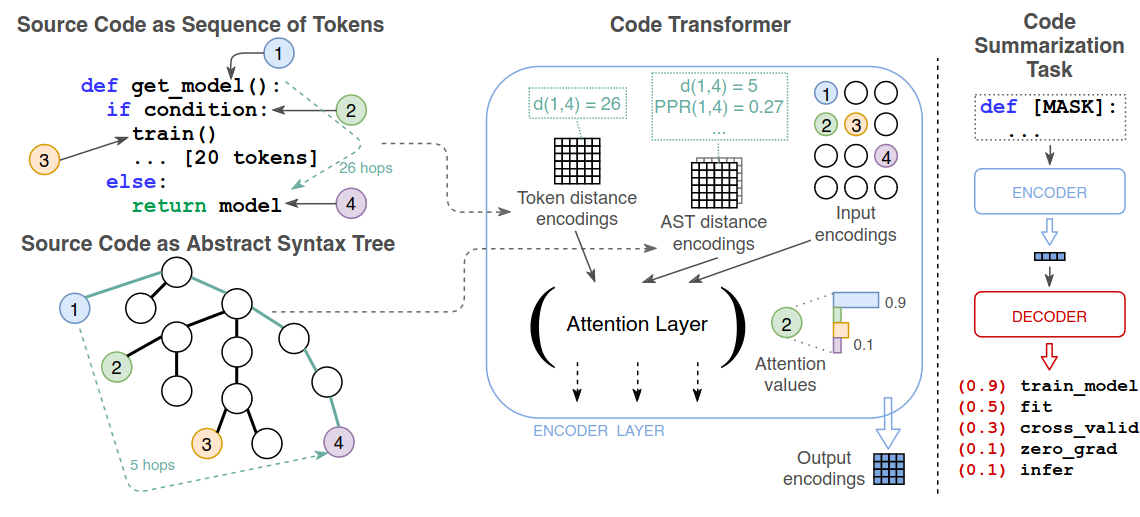
\includegraphics[width=\textwidth]{figuras/code-transformer.png}}
\caption{``\textbf{Left:} Sequence (Context) and AST (Structure) representation of an input code snippet. \textbf{Center:} The CODE TRANSFORMER jointly leverages the sequence of tokens and the Abstract Syntax Tree to learn expressive representations of source code. In addition to the input token and node embeddings the model uses different distances between the tokens, e.g., shortest paths on the AST or personalized PageRank, to reason about their relative positions. The output embeddings can be used for downstream tasks such as code summarization \textbf{(right)}.'' \citep{code_transformer}}
\label{fig:codetransf}
\end{figure}







\section{Github Copilot X, Code Whisperer and Code Assistants}

In recent years there has been an influx of code assisting tools based on machine learning models. Most of them are closed source with no details about their implementation, such as TabNine's autocompleter \citep{tabnine}, Amazon's CodeWhisperer code assistant \citep{whisperer} and Microsoft's Copilot, or even platform specific such as Replit's Ghostwriter \citep{ghost_writer}. With the release of Copilot X \citep{copilotx}, the latest iteration of the GitHub Copilot project, some details were made available to the public about its implementation but not that much is known besides the fact that they claim to use GPT-4.


Another interesting experimental project by the \citet{brushes} team are the code brushes , where the user can choose ``brushes'' to apply certain effects on code, such as making it more readable, adding types or including debugging statements, among other code transformations. Most of its brush operations are essentially refactorings, small operations with the intent of making code more readable and maintainable without altering its behavior. 
However, currently there is not a brush for function extractions.


These ``AI'' assisted tools have managed to achieve great popularity among developers, however due to their closed source nature, wait lists and paywalls, it is difficult to even try to compare them with the work developed in this project since we lack access to them and the knowledge about what is going on under the hood. The more flexible systems based on LLMs, such as Copilot X, could be tailored through prompts to attempt to realize function extractions, but doing so in a programmatical manner to measure its performance would be a challenge. We are still awaiting for the opportunity to test the Copilot X but even if we had access to it and achieved a good performance in the function extraction task there would be the doubt about the nature of this performance: is the model performing well or is it simply overfitted? Since our training, validation and test sets come from Java projects in GitHub, it would be hard to determine if the test files were never used during the Copilot X training leading to data snooping.

For these reasons, there won't be any comparisons between these tools and the models we developed, however we felt the need to mention them for the sake of completeness.





\section{Machine learning based code refactoring prediction}
\label{sec:mauricio}

Work from \citet{mauricio_paper} has shown that supervised machine learning methods are effective in predicting refactoring opportunities and, more importantly, such models can accurately model the refactoring recommendation problem. 
For this task, process and ownership metrics where shown to be essential for model creation, were the ownership metrics correspond to the suite proposed by \citet{ownership_metrics} and the process metrics are: quantity of commits, number of bug fixes, the sum of lines added, the sum of lines removed,  and number of previous refactoring operations.

Albeit an important milestone, it's important to emphasize that the model proposed on this work was only capable of predicting refactoring \textit{types} and \textit{opportunities}, not the refactoring operations themselves.
The models generated have also been shown to be robust with context change, i.e. a model trained in one context (e.g. Apache projects) can accurately predict refactoring opportunities on another context/project (e.g. F-droid projects). In Table~\ref{table:mau_modelos} we present the performance of the different models trained by \citet{mauricio_paper}.




\begin{table}[!ht]
\centering
\caption{The precision (Pr), recall (Re), and accuracy (Acc) of the different machine learning models, when trained and tested in the entire dataset (Apache + F-Droid + GitHub). Values range between [0,1]  \citep{mauricio_paper}. Table reconstructed from the original paper.}

\label{table:mau_modelos}

\resizebox{\textwidth}{!}{

\begin{tabular}{l c c c|c c c|c c c|c c c|c c c|c c c}
\hline & \multicolumn{3}{c}{$\begin{array}{c}\text { \textbf{Logistic} } \\
\text { \textbf{Regression} }\end{array}$} & \multicolumn{3}{c}{$\begin{array}{c}\text { \textbf{SVM} } \\
\text { \textbf{(linear)} }\end{array}$} & \multicolumn{3}{c}{$\begin{array}{c}\text { \textbf{Naive Bayes} } \\
\text {\textbf{ (gaussian)} }\end{array}$} & \multicolumn{3}{c}{$\begin{array}{c}\text { \textbf{Decision} } \\
\text { \textbf{Tree} }\end{array}$} & \multicolumn{3}{c}{$\begin{array}{c}\text { \textbf{Random} } \\
\text { \textbf{Forest} }\end{array}$} & \multicolumn{3}{c}{$\begin{array}{c}\text { \textbf{Neural} } \\
\text { \textbf{Network} }\end{array}$} \\
\hline & $\operatorname{Pr}$ & $\operatorname{Re}$ & $\operatorname{Acc}$ & $\operatorname{Pr}$ & $\operatorname{Re}$ & $\operatorname{Acc}$ & $\operatorname{Pr}$ & $\operatorname{Re}$ & $\operatorname{Acc}$ & $\operatorname{Pr}$ & $\operatorname{Re}$ & $\operatorname{Acc}$ & $\operatorname{Pr}$ & $\operatorname{Re}$ & $\operatorname{Acc}$ & $\operatorname{Pr}$ & $\operatorname{Re}$ & $\operatorname{Acc}$ \\
\hline \multicolumn{19}{l}{ \textbf{Class-level refactorings} } \\
Extract Class & 0.78 & 0.91 & 0.82 & 0.77 & 0.95 & 0.83 & 0.55 & 0.93 & 0.59 & 0.82 & 0.89 & 0.85 & 0.85 & 0.93 & 0.89 & 0.80 & 0.94 & 0.85 \\
 Extract Interface & 0.83 & 0.93 & 0.87 & 0.82 & 0.94 & 0.87 & 0.58 & 0.94 & 0.63 & 0.90 & 0.88 & 0.89 & 0.93 & 0.92 & 0.92 & 0.88 & 0.90 & 0.89 \\
 Extract Subclass & 0.85 & 0.94 & 0.89 & 0.84 & 0.95 & 0.88 & 0.59 & 0.95 & 0.64 & 0.88 & 0.92 & 0.90 & 0.92 & 0.94 & 0.93 & 0.84 & 0.97 & 0.89 \\
 Extract Superclass & 0.84 & 0.94 & 0.88 & 0.83 & 0.95 & 0.88 & 0.60 & 0.96 & 0.66 & 0.89 & 0.92 & 0.90 & 0.91 & 0.93 & 0.92 & 0.86 & 0.94 & 0.89 \\
 Move And Rename Class & 0.89 & 0.93 & 0.91 & 0.88 & 0.95 & 0.91 & 0.69 & 0.94 & 0.76 & 0.92 & 0.95 & 0.94 & 0.95 & 0.95 & 0.95 & 0.88 & 0.94 & 0.91 \\
 Move Class & 0.92 & 0.96 & 0.94 & 0.90 & 0.97 & 0.93 & 0.67 & 0.96 & 0.74 & 0.98 & 0.96 & 0.97 & 0.98 & 0.97 & 0.98 & 0.92 & 0.97 & 0.94 \\
 Rename Class & 0.87 & 0.94 & 0.90 & 0.86 & 0.96 & 0.90 & 0.63 & 0.96 & 0.69 & 0.94 & 0.91 & 0.93 & 0.95 & 0.94 & 0.94 & 0.88 & 0.94 & 0.91 \\
\hline \multicolumn{19}{l}{ \textbf{Method-level refactorings} } \\
 Extract And Move Method & 0.72 & 0.86 & 0.77 & 0.71 & 0.89 & 0.76 & 0.63 & 0.94 & 0.69 & 0.85 & 0.75 & 0.81 & 0.90 & 0.81 & 0.86 & 0.79 & 0.85 & 0.81 \\
 Extract Method & 0.80 & 0.87 & 0.82 & 0.77 & 0.88 & 0.80 & 0.65 & 0.95 & 0.70 & 0.81 & 0.86 & 0.82 & 0.80 & 0.92 & 0.84 & 0.84 & 0.84 & 0.84 \\
 Inline Method & 0.72 & 0.88 & 0.77 & 0.71 & 0.89 & 0.77 & 0.61 & 0.94 & 0.67 & 0.94 & 0.87 & 0.90 & 0.97 & 0.97 & 0.97 & 0.77 & 0.85 & 0.80 \\
 Move Method & 0.72 & 0.87 & 0.76 & 0.71 & 0.89 & 0.76 & 0.63 & 0.93 & 0.70 & 0.98 & 0.87 & 0.93 & 0.99 & 0.98 & 0.99 & 0.76 & 0.84 & 0.78 \\
 Pull Up Method & 0.78 & 0.90 & 0.82 & 0.77 & 0.91 & 0.82 & 0.68 & 0.95 & 0.75 & 0.96 & 0.88 & 0.92 & 0.99 & 0.94 & 0.96 & 0.82 & 0.87 & 0.84 \\
 Push Down Method & 0.75 & 0.89 & 0.80 & 0.75 & 0.90 & 0.80 & 0.66 & 0.94 & 0.73 & 0.97 & 0.76 & 0.87 & 0.97 & 0.83 & 0.90 & 0.81 & 0.92 & 0.85 \\
 Rename Method & 0.77 & 0.89 & 0.80 & 0.76 & 0.90 & 0.80 & 0.65 & 0.95 & 0.71 & 0.78 & 0.84 & 0.80 & 0.79 & 0.85 & 0.81 & 0.81 & 0.82 & 0.81 \\
\hline \multicolumn{19}{l}{\textbf{Variable-level refactorings} } \\
Extract Variable & 0.80 & 0.83 & 0.82 & 0.80 & 0.83 & 0.82 & 0.62 & 0.94 & 0.68 & 0.82 & 0.83 & 0.82 & 0.90 & 0.83 & 0.87 & 0.84 & 0.89 & 0.86 \\
Inline Variable & 0.76 & 0.86 & 0.79 & 0.75 & 0.87 & 0.79 & 0.60 & 0.94 & 0.66 & 0.91 & 0.85 & 0.88 & 0.94 & 0.96 & 0.95 & 0.81 & 0.82 & 0.82 \\
Parameterize Variable & 0.75 & 0.85 & 0.79 & 0.74 & 0.86 & 0.78 & 0.59 & 0.94 & 0.65 & 0.88 & 0.81 & 0.85 & 0.93 & 0.92 & 0.92 & 0.80 & 0.83 & 0.81\\
Rename Parameter & 0.79 & 0.88 & 0.83 & 0.80 & 0.88 & 0.83 & 0.65 & 0.95 & 0.71 & 0.99 & 0.92 & 0.95 & 0.99 & 0.99 & 0.99 & 0.82 & 0.87 & 0.84 \\
Rename Variable & 0.77 & 0.85 & 0.80 & 0.76 & 0.86 & 0.79 & 0.58 & 0.92 & 0.63 & 0.99 & 0.93 & 0.96 & 1.00 & 0.99 & 0.99 & 0.81 & 0.84 & 0.82 \\
Replace Variable With Attribute & 0.79 & 0.88 & 0.82 & 0.78 & 0.89 & 0.82 & 0.64 & 0.95 & 0.71 & 0.90 & 0.84 & 0.88 & 0.94 & 0.92 & 0.93 & 0.79 & 0.92 & 0.84 \\
\hline
\end{tabular}
}
\end{table}



\subsection{DataSet}
\label{sec:mauricio_dataset}



\citet{mauricio_paper} constructed a 40Gb dataset of source code from Java libraries, their entire Git commits history and metrics calculated on each commit. This was built upon 3 different ecosystems: Apache, F-droid and Github; an outline of the dataset can be referenced in Table~\ref{table:mau_dataset}.
The Apache ecosystem is composed of all Java-based Apache software projects supported by the \citet{apache} and the \citet{fdroid} ecosystem is a repository of FOSS Android mobile apps. Lastly, the GitHub ecosystem is composed of the first 10,000 most starred Java projects hosted on GitHub (removing duplicates of the Apache and F-Droid cohorts that are also hosted on GitHub as mirrors).

\begin{table}[!ht]
\caption{Number of projects and commits per ecosystem and in total.}
\label{table:mau_dataset}

\begin{tabular}{l|c|c}
               & Number of projects & Total number of commits \\ \hline
Apache         & 844                & 1,471,203                 \\
F-Droid        & 1,233               & 814,418                  \\
GitHub         & 9,072               & 6,517,597                 \\ \hline
\textbf{Total} & 11,149              & 8,803,218                
\end{tabular}
\end{table}




By utilizing RefactoringMiner \citep{refactoringminer_2.0}, the current state-of-the-art tool for refactoring identification in Java, on only the production files they were able to identify 20 different refactoring classes with varying number of occurrences, e.g. the dataset contains $327,493$ instances of the \textit{Extract Method} refactoring class but only 654 of \textit{Move and Rename Class}. Table~\ref{table:mau_refacs} presents an overview of each refactoring instance obtained by different cohort and refactoring type.


At the same time that the refactoring instances were identified, non-refactoring instances and metrics for both of them were also obtained. 



\begin{table}[!ht]
\centering
\caption{The number of instances of refactoring and non-refactoring classes used in \citet{mauricio_paper}. Table reconstructed from the original paper, our emphasis.}
\label{table:mau_refacs}

\resizebox{.7\textwidth}{!}{
\begin{tabular}{lrrrr} 
& All & Apache & GitHub & F-Droid \\
\hline \textbf{Class-level refactorings} & & & & \\
Extract Class & 41,191 & 6,658 & 31,729 & 2,804 \\
Extract Interface & 10,495 & 2,363 & 7,775 & 357 \\
Extract Subclass & 6,436 & 1,302 & 4,929 & 205 \\
Extract Superclass & 26,814 & 5,228 & 20,027 & 1,559 \\
Move And Rename Class & 654 & 87 & 545 & 22 \\
Move Class & 49,815 & 16,413 & 32,259 & 1,143 \\
Rename Class & 3,991 & 557 & 3,287 & 147 \\
\hline \textbf{Method-level refactoring}s & & & & \\
Extract And Move Method& 9,723 & 1,816 & 7,273 & 634 \\
\rowcolor{backquote}Extract Method & 327,493 & 61,280 & 243,011 & 23,202 \\
Inline Method & 53,827 & 10,027 & 40,087 & 3,713 \\
Move Method & 163,078 & 26,592 & 124,411 & 12,075 \\
Pull Up Method & 155,076 & 32,646 & 116,953 & 5,477 \\
Push Down Method & 62,630 & 12,933 & 47,767 & 1,930 \\
\rowcolor{backquote}Rename Method & 427,935 & 65,667 & 340,304 & 21,964 \\
\hline \textbf{Variable-level refactorings} & & & & \\
Extract Variable & 6,709 & 1,587 & 4,744 & 378 \\
Inline Variable & 30,894 & 5,616 & 23,126 & 2,152 \\
Parameterize Variable & 22,537 & 4,640 & 16,542 & 1,355 \\
Rename Parameter & 33,6751 & 61,246 & 261,186 & 14,319 \\
Rename Variable & 324,955 & 57,086 & 250,076 & 17,793 \\
Replace Variable w/ Attr. & 25,894 & 3,674 & 18,224 & 3,996 \\
\hline \textbf{Non-refactoring instances} & & & & \\
Class-level & 10,692 & 1,189 & 8,043 & 1,460 \\
Method-level & 293,467 & 38,708 & 236,060 & 18,699 \\
Variable-level & 702,494 & 136,010 & 47,811 & 518,673
\end{tabular}
 }
\end{table}


%!TeX root=../tese.tex
%("dica" para o editor de texto: este arquivo é parte de um documento maior)
% para saber mais: https://tex.stackexchange.com/q/78101


% One of our working hypothesis is that a refactoring commit is only a refactoring commit, that is no new features have been added nor there are other code alterations in this single commit. Even if a refactoring commit has other alterations to the code base, those alterations may not be in the same file of the refactoring or even in the same function so with some processing we should be able to obtain ``pure'' refactoring commits for a reasonable portion of our dataset.


\chapter{(Re)Building a Dataset}
 Originally, this project was conceived as a partnership with the TUDelft where we would build upon their previous work by training our models on the dataset they build in \citet{mauricio_paper} and that we previously presented in Section~\ref{sec:mauricio_dataset}. However once we received the full dataset %, after months of wait,  
  we realized that it was not suitable for our needs. Since they did not capture any information regarding which lines were extracted in the function extractions nor any other more minute details about where and how  exactly the refactorings occurred, there was no way to train a supervised machine learning model. The dataset could still be used for unsupervised approaches and other less granular tasks, however we decided to collect our own dataset to be able to accomplish our original objectives. We briefly explored the possibility of leveraging the existing dataset to obtain the extracted lines but we reached the conclusion that scrapping them from scratch would be simpler and faster.
This heavily impacted our proposed timeline since there was a need to create an usable dataset from scratch. Utilizing a list of over 40.000 Java repositories %from\citet{lista_repos} 
provided by SERG - TUDelft, and made available at \citet{lista_repos},
we created a data pipeline with a tool called RefactoringMiner \citep{refactoringminer_2.0} at its core. 
In this chapter we will detail how we constructed this dataset and the reasoning behind some of our decisions, this new objective of creating a dataset instead of using a pre-built one led us to a series of new decisions. The first of them being our decision to maintain our objective of working with function extractions. 
If we reference Table~\ref{table:mau_refacs} one might notice that the most common refactoring was of the \textit{Rename Method} type. Although they were not originally published with this sole task or problem formulation in mind, code2vec, code2seq and code transformer achieve an impressive performance in this task \citep{code2vec, code2seq, code_transformer}.  In contrast, the second most common refactoring was of the type \textit{Extract Method} and to the best of our knowledge there is no model for automating this refactoring. Tackling this new and interesting task was the biggest motivator behind our choice of working with function extractions instead of other less common refactorings.

% \footnote{If the cohorts analyzed by \citet{mauricio_paper} are a big and general enough segment of Java projects to be considered representative of Java projects and/or Java programmers at large could be cause for debate, however investigating this would be out of the scope for this project.}

 This leads us to the next decision in our data building task, what tool should we use to obtain function extractions?


 \section{RefactoringMiner}


To create a model for automatic function extraction our dataset needs to have examples of function extractions with the lines extracted being appropriately tagged. Doing so by hand would be error prone and time consuming, so tools crafted to ``mine'' git repositories for such refactorings are commonly used.

One of such tools is RefactoringMiner 2.0. It can detect 40 different refactoring types through rules based on statement mapping information and AST node replacements. In its 1.0 version \citep{refactoring_miner1} it attained a state of the art performance and, maybe more importantly, introduced a refactoring oracle of validated refactoring instances, providing a new rigorous benchmark for the field. RefactoringMiner 2.0 expanded this oracle into 7,226 true positives in total, for 40 different refactoring types detected
by one (minimum) up to six (maximum) different tools. These refactorings were mined from 536 commits from 185 open-source Java projects hosted on GitHub.
Another important feature present in RefactoringMiner 2.0 is the ability to detect nested refactorings:

\begin{myquote}
\textit{A refactoring operation that takes place in code resulting from the application of another refactoring operation is a nested refactoring. For example, the renaming or extraction of local variables inside the body of an extracted method are nested refactoring operations[...].}
\\\citet{refactoringminer_2.0}
\end{myquote}

Fig.~\ref{img:nested_refac} shows a real case of nested extract method refactorings. 

\begin{figure}[!ht]
\centerline{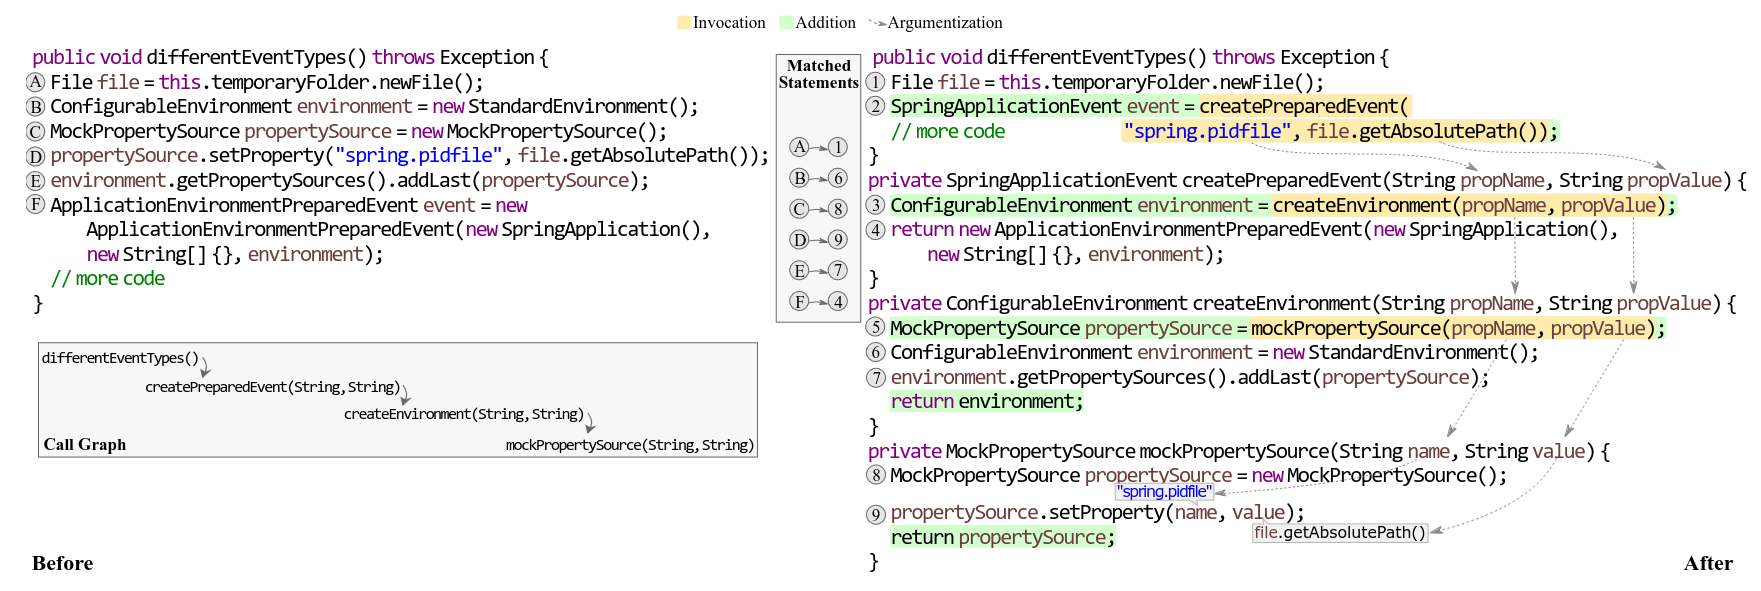
\includegraphics[width=1.2\textwidth]{figuras/nested_refacs.png}   }
\caption{Nested extract method refactorings mined from \url{github.com/spring-projects/spring-boot/commit/becce}. There
are 3 levels of nested extracted methods with each extracted
method calling the subsequent one. Image from \citet{refactoringminer_2.0}.}
\label{img:nested_refac}
\end{figure}

This tool is the same one utilized to create the dataset described in Section~\ref{sec:mauricio_dataset}, so when we were choosing a refactoring detection tool it was naturally considered. But with the release of new tools and versions we were interested if RefactoringMiner could still be considered the state of the art in all Java refactoring detections so we explored the possibility of using other tools such as RefDiff \citep{silva2020refdiff} and RefDetect \citep{moghadam2021refdetect}. However, we found that specifically for function extractions RefactoringMiner still outperforms its competitors, as can be seen in Tables~\ref{img:tabela_refdetect_refacminer} and \ref{img:tabela_refminer_refdiff}.


\begin{table}[!ht]
\centerline{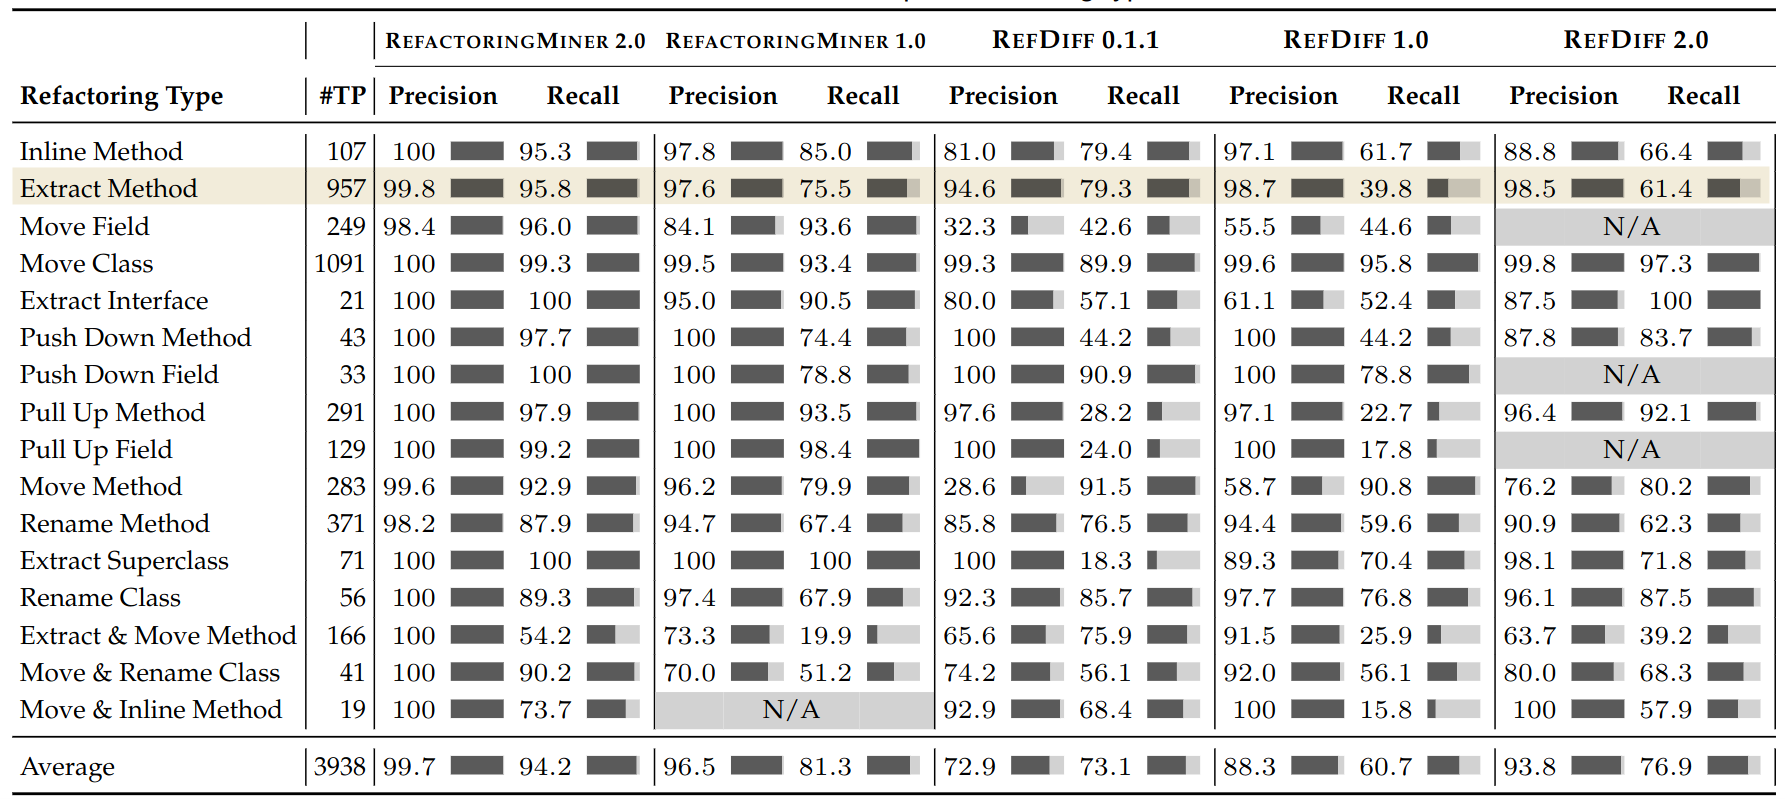
\includegraphics[width=\textwidth]{figuras/tabela_refminer_refdiff.png}   }
\caption{Precision and recall per refactoring type. Values calculated based on a refactoring
oracle of validated instances containing 7,226 true
positives in total, for 40 different refactoring types detected
by one (minimum) up to six (maximum) different tools. Table  and caption from \citet{refactoringminer_2.0}, our highlight.}
\label{img:tabela_refminer_refdiff}
\end{table}

\begin{table}[!ht]
\centerline{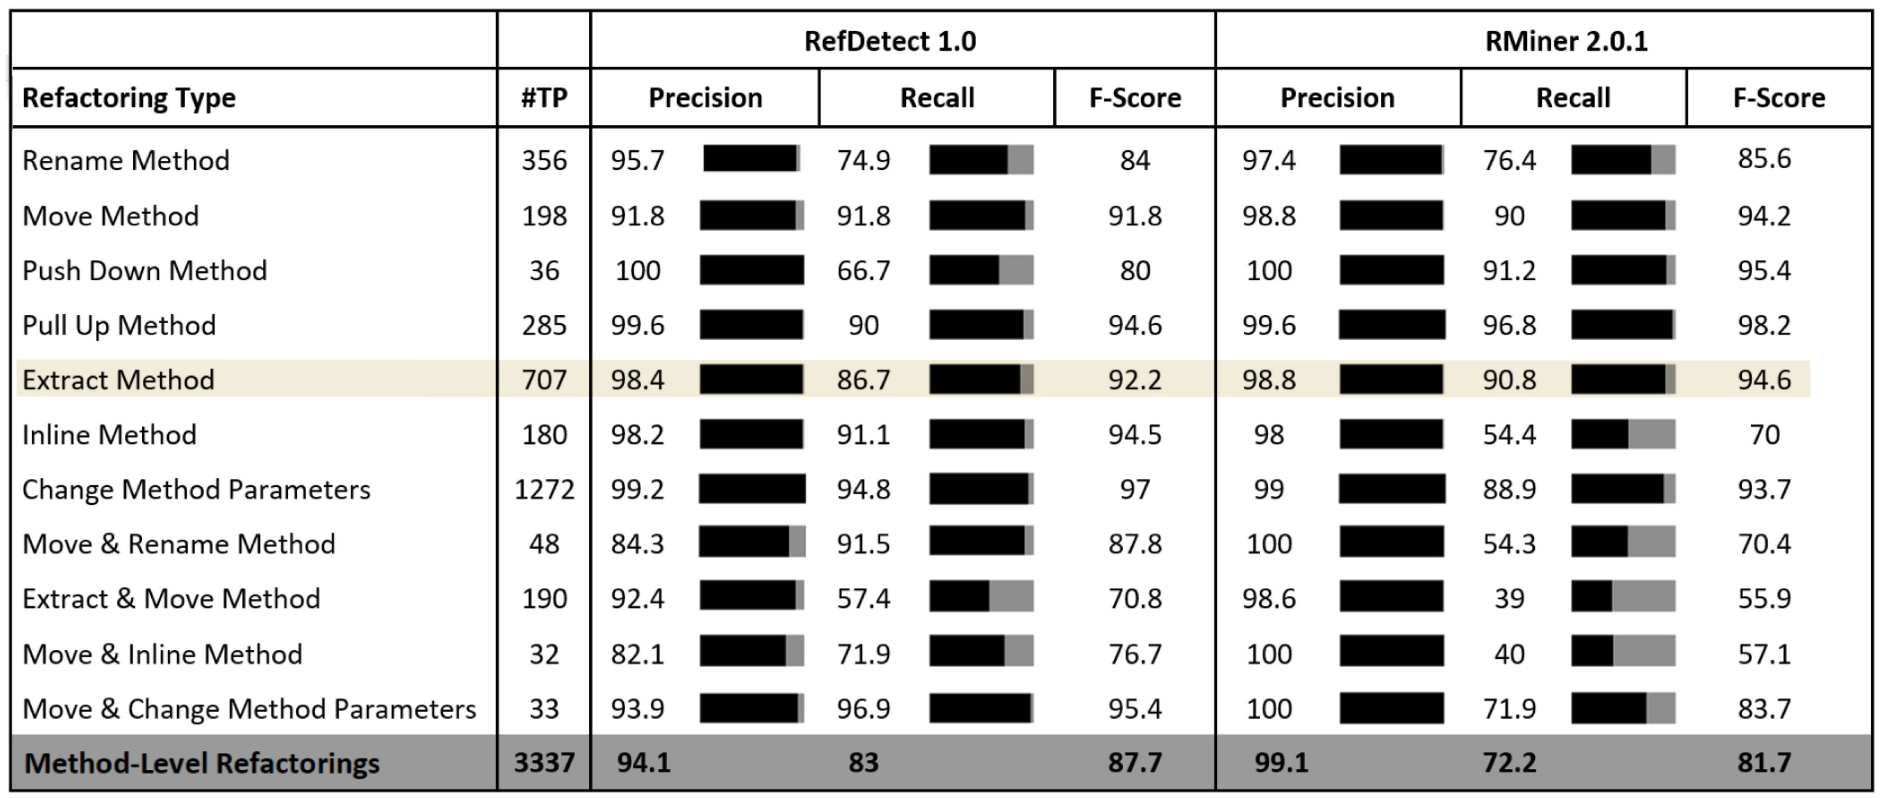
\includegraphics[width=\textwidth]{figuras/tabela_refdetect_refacminer.png}   }
\caption{Precision, recall and f-score results per method-level refactoring type. Values calculated based on a refactoring
oracle of validated instances from \citet{refactoringminer_2.0}, containing 7,226 true
positives in total for 40 different refactoring types detected
by one (minimum) up to six (maximum) different tools. Table from \citet{moghadam2021refdetect}, our highlight.}
\label{img:tabela_refdetect_refacminer}
\end{table}


With this, we also decided to utilize RefactoringMiner to build our dataset, but if in future work we expand on the refactorings we deal with or the targeted programming languages, RefDetect, a multilingual refactoring detection tool, may be a better pick:  

\begin{myquote}
\textit{RefDetect clearly outperformed R\textbf{(efactoring)}Miner in method and class based refactorings, achieving f-scores respectively of 87.7\% vs. 81.7\% for method-level refactorings and 92.1\% vs. 86.9\% for class-level refactorings.}
\\\citet{moghadam2021refdetect}
\end{myquote}


\section{Pipeline}

The overall structure of our pipeline is quite simple, as can be seen in Fig.~\ref{pipeline}. We start by cloning over 40.000 repositories of Java projects, these projects come from a list curated by the SERG group of the TUDelft university and available at \citet{lista_repos}.
With the repositories cloned we can start mining refactorings with RefactoringMiner. 
RefactoringMiner outputs one json file per mined repository, so our next step is to process all these json files and filter only the relevant features into our SQLite database. For this project we are only interested in function extraction refactorings, so we drop every other refactoring found. Then we check if the function extraction found covers a continuous span of lines, and if they are not continuous if maybe only blank lines or comments separate the continuous chunks; Fig.~\ref{img:dfa} illustrates this process with a Discrete Finite Automata. Lastly, we exclude any refactorings that happen at the same function in a same git commit. We do so to simplify our model and training process, we believe keeping these refactorings would negatively impact our performance and raise an issue of non determinism since multiple predictions could be found to be correct.

\begin{figure}[!ht]
\centerline{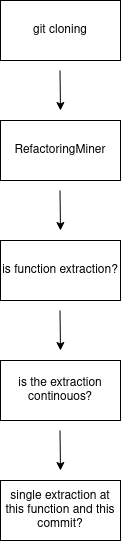
\includegraphics[scale=0.50]{pipeline.png}   }
\caption{A short visualization of the steps present in our data pipeline.}
\label{pipeline}
\end{figure}


The entirety of the code utilized in the construction of this dataset is available in Appendix~\ref{an:code_data}.




\begin{figure}[!ht]
\centerline{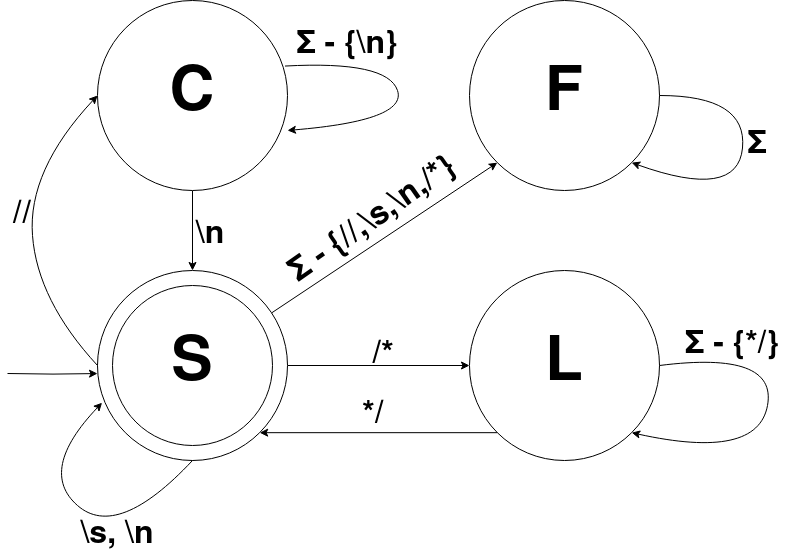
\includegraphics[width=0.6\textwidth]{figuras/DFA.png}   }
\caption{A Discrete Finite Automata that detects if any of the lines analyzed is not a comment or blank line. For the sake of simplicity and illustration, let us consider that symbols such as ``//'', ``/*'', ``*/'', ``\textbackslash n'' and ``\textbackslash s'' are single characters. Building a real DFA that breaks each of these ``signals'' into their constituent characters would increase the complexity of the system and loose its meaning as an illustration to clarify our data processing.
Following convention, $\Sigma$ represents the alphabet of this DFA, i.e. the set of all valid characters in the java language. State \textbf{S} represents blank lines, the \textbf{C} state represents comments and \textbf{L} long comments, lastly the \textbf{F} state represents a failure, once something that does not constitute a comment, long comment or blank line is detected the process gets stuck in the \textbf{F} state unable to ever reach the accepting state 
\textbf{S}.}
\label{img:dfa}
\end{figure}

\section{Exploration of the dataset}

Even though we started with a list of 49,982 Java repositories, we only managed to obtain function extractions from 19,936 of them. Many factors played a part in this, such as problematic encodings when processing the files, repositories not found due to renaming or migration, RefactoringMiner limitations, only refactorings other than function extraction found or even repositories that weren't purely written in Java (some were mostly written in Kotlin with just a few files in Java, for example).

However, even with all these issues we obtained 523,667 different instances of function extraction, an increase of over 60\% in comparison with the dataset we originally intended to use from \citet{mauricio_paper}. Interestingly, over 80\% of the function extractions found  are continuous, given the diverse range of Java projects used in this analysis we believe this should be a good approximation to the real proportion of continuous function extractions in relation to non-continuous. This further solidified our decision to focus on only continuous extractions for our model, since they are not only simpler to train but also arguably a more useful and actionable suggestion for developers.



%!TeX root=../tese.tex
%("dica" para o editor de texto: este arquivo é parte de um documento maior)
% para saber mais: https://tex.stackexchange.com/q/78101


\chapter{Models}
\label{chap:models}

In this chapter we will be exploring the different components of the models we developed and the motivation behind our decisions. Lastly the hyper-parameters choice and the optimization of the different models trained  will also be briefly explored. 



\section{Embeddings}

To create our function extraction models we need to be able to calculate an embedding for code functions. However, none of the previously explored code embeddings in Chapter~\ref{chap:related_work} are granular enough for our needs, they expect whole functions while we need to be able to at the very least create embeddings per line of code. Exploring the literature, in particular \citet{allamanis2018survey} which presents a table of over 30 code embedding generators for a diverse range of tasks, we were not able to find a fitting embedding. One of our original objectives was to develop our own code embedding for this task, however due to time constraints caused by the dataset delay this was no longer feasible.



So, once again leveraging the idea of naturalness of programming languages that we introduced in Chapter~\ref{chap:intro} we opted to utilize embeddings for natural languages --- in particular english --- to represent our code.


There were two main types of embeddings tested in this project: the more traditional GloVe based embeddings and the transformer based embeddings that we had the opportunity of exploring during the semester abroad at TUDelft thanks to the FAPESP BEPE program. Both embeddings are sentence embeddings, i.e. each line of code will have its own vector embedding. Here we will give a short  overview of how these embeddings work and how they were built.



\subsubsection{Transformer based}


Following our initial goal of exploring the use of transformers for refactoring tasks we arrived at two main approaches: utilizing transformers in our embedding and/or as our model. However, due to our time constraints imposed by our need to create our dataset from scratch, we focused on utilizing transformer based embeddings as the first step since adapting the dataset to be compatible with training a transformer model would be an extremely manual and time consuming process. Another relevant point is the maxim of ``garbage in garbage out'', that essentially states that if your data is bad your results will also be bad. We concluded that it would be more beneficial to first make sure that we have at least one reasonable embedding for our code before we start investing such a huge amount of our scarce time in adopting this new architecture. Unfortunately, by the time we finished exploring the use of transformer based embeddings, there was no feasible way of training a transformer model in the remaining time of the BEPE project. Therefore, in this section we will be exploring the use of transformer based embeddings and their performance compared to more traditional embeddings.


Among the many embedding options available for our analysis we chose to utilize the transformer based models of the SBERT project \citep{sbert_paper}. Until recently this project was referred to as the state of the art in many tasks involving sentence embeddings, furthermore it possesses embeddings trained through a diverse number of transformer based architectures with most of them being more computationally efficient when compared to other models such as BERT \citep{BERT} or RoBERTa \citep{roberta}.



In Fig.~\ref{embeddings}, also available as an interactive table at \citet{link_sbert_tabela}, we can see the main 13 models of interest available in the SBERT project and some metrics regarding them. Due to our time constraints we were forced to select only a few of these embeddings for our experiment, since they may take an entire day to train a single epoch. From this list we discarded all models solely trained on Q\&A datasets since they are too distinct from our real objective and other models that were too derivative of another model already present in the list such as \textit{all-MiniLM-L6-v2} (half the layers of \textit{all-MiniLM-L12-v2}), \textit{distiluse-base-multilingual-cased-v2} (trained in an additional 35 languages in comparison to \textit{distiluse-base-multilingual-cased-v1} but since most of our Java files are believed to be written in english we don't believe this would bring us significant gains in performance) and \textit{paraphrase-multilingual-mpnet-base-v2} (a slow and more inefficient version of \textit{all-mpnet-base-v2} that was trained in a smaller and more specific dataset). 


\begin{figure}[!ht]
\centerline{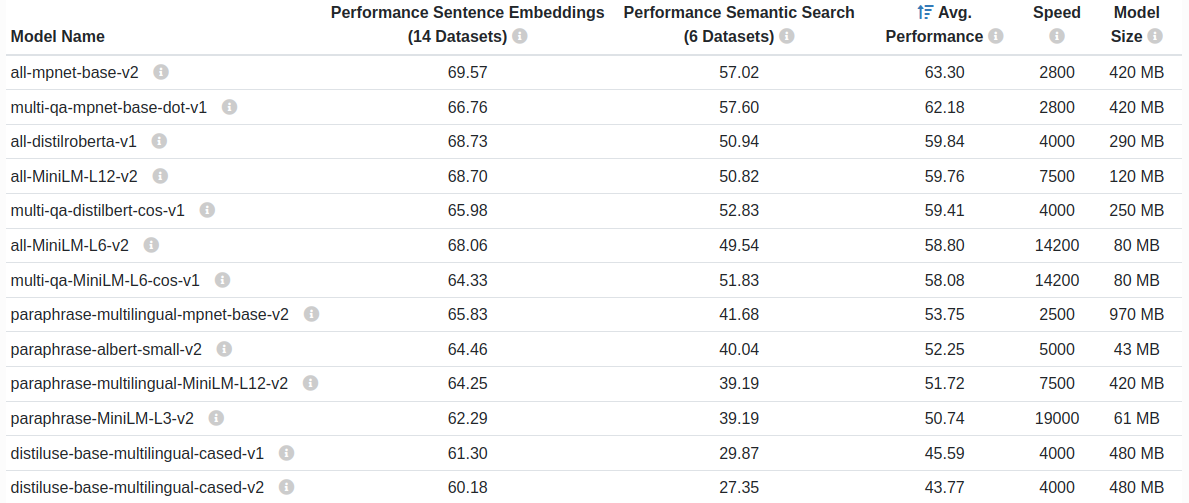
\includegraphics[scale=0.62]{embeddings.png}   }
\caption{Table of 13 embedding models available in the SBERT project and some metrics regarding them. \citep{link_sbert_tabela}}
\label{embeddings}
\end{figure}


After short-listing the available embeddings we were left with 7 embeddings to test out:
\begin{itemize}
    \item all-mpnet-base-v2 \citep{mpnet} \href{https://huggingface.co/sentence-transformers/all-mpnet-base-v2}{(Model Card)}
    \item all-distilroberta-v1 \citep{roberta, distillbert} \href{https://huggingface.co/sentence-transformers/all-distilroberta-v1}{(Model Card)}
    \item all-MiniLM-L12-v2 \citep{minilm}  \href{https://huggingface.co/sentence-transformers/all-MiniLM-L12-v2}{(Model Card)}
    \item paraphrase-albert-small-v2 \citep{albert}  \href{https://huggingface.co/sentence-transformers/paraphrase-albert-small-v2}{(Model Card)}
    \item paraphrase-multilingual-MiniLM-L12-v2 \citep{minilm}  \href{https://huggingface.co/sentence-transformers/paraphrase-multilingual-MiniLM-L12-v2}{(Model Card)}
    \item paraphrase-MiniLM-L3-v2 \citep{minilm}  \href{https://huggingface.co/sentence-transformers/paraphrase-MiniLM-L3-v2}{(Model Card)}
    \item distiluse-base-multilingual-cased-v1 \citep{distillbert}  \href{https://huggingface.co/sentence-transformers/distiluse-base-multilingual-cased-v1}{(Model Card)}
\end{itemize}


\subsubsection{GloVe}

GloVe \citep{glove} is a more traditional model that combines the advantages of two model families, local context windows and global matrix factorization. 
The model produces a vector space with meaningful sub-structure by leveraging statistical information in an efficient manner when training only on the nonzero elements in a word-word co-occurrence matrix, rather than on individual context windows in a large corpus or on the entire sparse matrix. 

At the time this method was published it attained state-of-the-art performance on the word analogy task, and outperformed other methods (such as word2vec) on several word similarity tasks.



By utilizing GloVe we also have an interesting counter-point to our transformer based embedding, we are essentially comparing an older and well established model that is still relevant even in this ever evolving field (the same cannot be said about bag-of-words for example) to what is essentially the more recent and generally successful approach.


By taking the average of the word embeddings of a sentence it is possible to generate an embedding for that sentence. This is what was done by \citet{sbert_site} in order to generate two GloVe sentence embedding models, one trained with 6 billion parameters and the other with 840 billion parameters.





\section{Architecture}

An important issue to be addressed here comes from a fundamental difference between natural languages and programming languages: even if a sentence in english has a grammatical mistake it is capable of transmitting meaning, of carrying a semantic value. The same cannot be said about a grammatically incorrect piece of code.
For this reason we are not able to blindly apply seq2seq NLP models on source code, we need to ensure that the code transformations we generate will not grammatically break the inputted code. To ensure the grammatical correctness of our refactoring we briefly explored the possibility of using language servers to intermediate our operations in Section~\ref{sec:lsp}.


Given this, our models simply needs to predict the line number of the start and end of the extracted linespan.


\begin{figure}[!ht]
\centering
\centerline{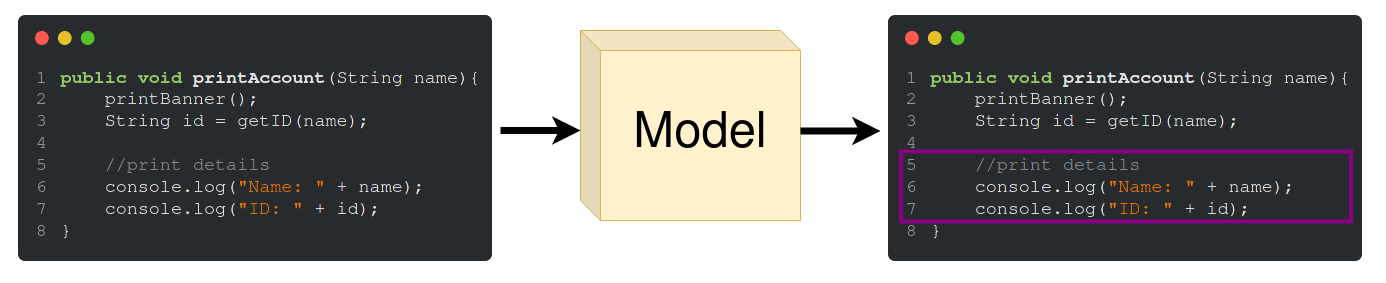
\includegraphics[scale=0.35]{figuras/modelo.png}}
\caption{Our model will receive the source code of a function definition that needs to be refactored and will output the line span that needs to be extracted. In this particular example the lines 5 to 7 of the \texttt{printAccount()} function need to be extracted.}
\label{modelo}
\end{figure}

\begin{figure}[!ht]
\centering
\centerline{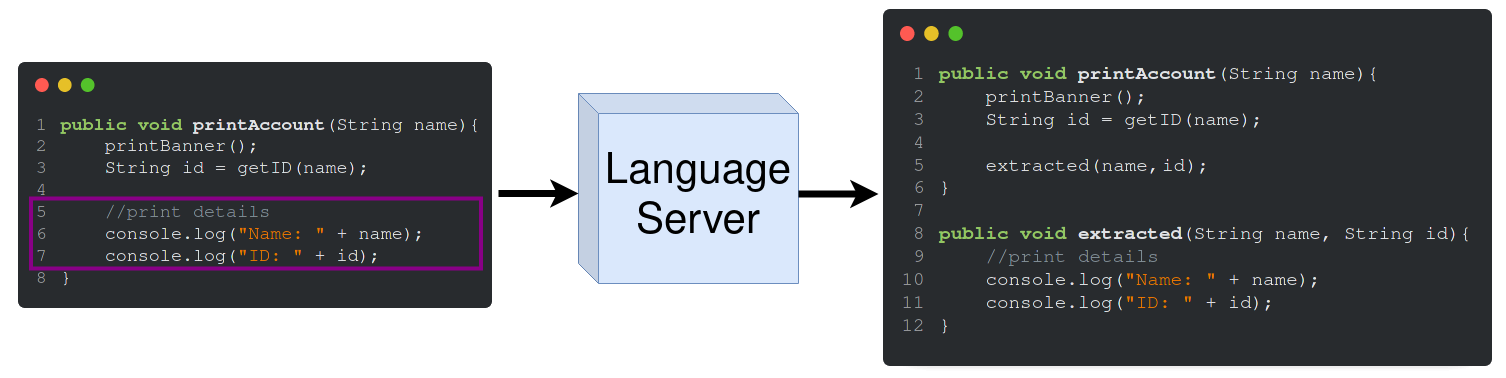
\includegraphics[scale=0.33]{figuras/lsp_refac.png}}
\caption{Once the line span of the extraction has been determined, the language server is contacted and it will be responsible for realizing the extraction and returning the refactored code. In this example the lines 5 to 7 are refactored by the language server and become the function \texttt{extracted()}.}
\label{lsp_refac}
\end{figure}

 In short, the model will be fed with the lines of a function one by one and it will generate as an output 2 pointers, one indicating the first line to be extracted and a second pointer indicating the last line to be extracted. Together these 2 pointers will define the line span to be refactored. Fig~\ref{modelo} presents a general illustration of our models, working as a black box, and Fig~\ref{lsp_refac} illustrates the refactoring done through a language server with the output of the black box model from Fig.~\ref{modelo}.



\subsubsection{Simple RNN}

Our first architecture is extremely simple; it consists of a LSTM layer that receives the embedded inputs and then passes on its hidden state to two different feedforward linear layers which will predict the start and end lines of the function extraction. 
As for the loss we chose the L1 distance function.



\subsubsection{Pointer Network (Ptr-Net)}

 Pointer Networks \citep{pointer} are a flexible encoder decoder model that utilizes attention to select one of the inputs as an output at each decoding step. As mentioned in Section~\ref{sec:ptrnet}, this model has been used in a variety of tasks that involve re-ordering and/or selecting elements of the inputted data. This is particularly useful in our case since our objective can be formulated as selecting which lines of an inputted function that need to be extracted, in particular at which line the extraction begins and ends. 

Our implementation of the pointer network utilizes a 1 layer LSTM as the encoder and another 1 layer LSTM as the decoder with the additive attention mechanism from \citet{bahdanau} tying them together. Lastly, to convert from the attention scores into the predicted lines we apply the softargmax function in order to apply the argmax function in a differentiable manner.



$$\textit{softargmax}(x)=\sum_i \frac{e^{\beta x_i}}{\sum_j e^{\beta x_j}}i$$

$\beta$ essentially controls how well this function approximate the argmax function, however a high enough $\beta$ will approximate it so well that back-propagation will start to fail. In Appendix~\ref{ap:beta} we present a brief exploration of the impact of $\beta$ on the model capability to learn. Luckily, our experiments did not detect any significant increase in performance by increasing $\beta$ over the value of 10, which is well below the point were back-propagation starts to fail.

We opted to use this function instead of the more commonly utilized softmax function in order to use the L1 loss instead of negative log likelihood loss. Since we are not predicting simple classes as our output, the error from missing the start of a refactoring by one line should be smaller than that of missing by 10 lines and this isn't possible with negative log likelihood. 
In Fig.~\ref{arquitetura} we can see an illustration of how this model works, particularly how the attention mechanism ``chooses'' the start and end of a function extraction. 





\begin{figure}[!ht]
\centerline{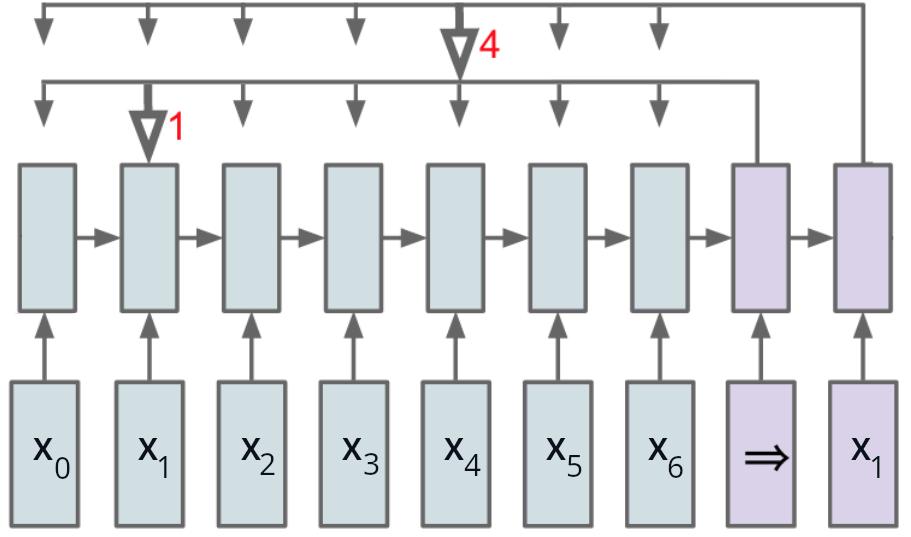
\includegraphics[scale=1.62]{arquitetura.png}   }
\caption{An illustration of how the model works, with green blocks representing the encoder and the purple ones the decoder. Each $x_i$ value fed to the encoder represents the embedding of a single line from the function being analyzed. The decoder receives as an input the hidden state from the last step (if available) and all the encoder hidden states, so to predict the last line to be extracted the decoder will receive all the hidden states from the encoder and the hidden state from last step that represents the first line to be extracted. Lastly, the attention mechanism is represented by the arrows pointing into the different encoder hidden states/inputs, the arrows may be seen as the final output of the model after the attention scores go through the softargmax function. So in this particular example being illustrated, the function is composed of 7 lines and it should go through an extraction of lines 1 through 4.}
\label{arquitetura}
\end{figure}




\section{Metrics}

When dealing with a well researched topic one is able to build upon previous knowledge and conventions in the area. However, to the best of our knowledge, there is no previous research that aims to automate the task of function extractions so we are faced with the challenge of defining how to best evaluate the quality of a predicted refactoring. In Section~\ref{sec:bleu} we explored a few common seq2seq metrics of NLP and their limitations, however none of the metrics presented are applicable for this particular use case, neither are the other metrics we could find in the literature. They may not be applicable to our particular use case but we may still take insights from them, such as BLEU's limitations that do not take into account if a sentence actually makes any semantic or grammatical sense. 

So without being able to resort to a readily available NLP metric we turned ourselves to typical code quality metrics, such as the ones presented in Section~\ref{sec:code_metrics}. Albeit these metrics can be useful in certain occasions we found them to be lacking for our needs. They can present a score of the code quality but by their very nature they are subjective since they try to give a concrete score to an abstract and subjective concept like code quality. Simply deciding which metric to use can bring vastly different results since not all of them are tailored towards the same issues and they do not operate on the same scales, comparing the pure score of different code metrics is akin to comparing apples to oranges.
Apart from that, our model performs only function extractions, the only code operation would be a transfer of code lines from an existing function to a newly created one, this would not bring a big impact in most code quality metrics. We could directly measure the size of functions instead of relying in more complicated code metrics but this would pose a new problem on itself, fewer lines of code does not necessarily equate to a better piece of code nor does a bigger extraction imply a better refactoring than a shorter one.
Besides, these metrics are not very actionable, they do not always present a clear path on how to improve the refactoring to maximize them.


Another early idea was to leverage unit tests to verify code integrity, however it is not guaranteed that all functions being refactored have unit tests nor that we would be able to easily identify them in a programmatic manner. Also, unless the linespan breaks a loop or some other flow control structure (which could be easily detected) the extraction would necessarily be a code preserving transformation so code integrity is not a concern.

Lastly we turned to classic ML metrics, such as accuracy.
We decided to utilize the binary accuracy, which is essentially equivalent to jaccard score, to measure how close the overlap between the predicted linespan and the ground truth is.

The jaccard coefficient is a measure of similarity between sets, defined as \citep{jaccard1912distribution}:
$$J(A,B) = \frac{|A \cap B|}{|A \cup B|} $$

An illustration of the jaccard index can be seen in Fig.~\ref{fig:jaccard_iou}.

\begin{figure}[!ht]
\centerline{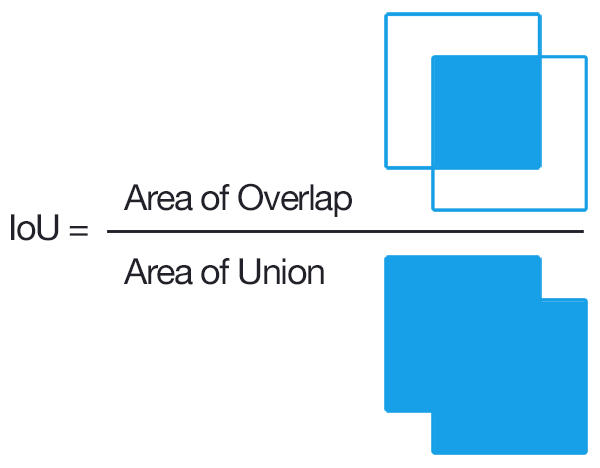
\includegraphics[scale=0.4]{figuras/iou.png}   }
\caption{A visual representation of the jaccard index. Image from \citet{iou}.}
\label{fig:jaccard_iou}
\end{figure}


Lastly, if an IDE plugin were to be implemented there would be the possibility of utilizing telemetry to evaluate user response to suggested refactorings. This would be a way to grasp the quality of suggested refactorings and to better understand when and why our model fails, however this is left for future work since such an endeavor was unfeasible given the time constraints of this project.


\section{Hyper-parameter choice}
\label{optuna}

Many scientific fields currently suffer from a reproducibility crisis \citep{reproducibility} and machine learning is no exception \citep{repro1, repro2, repro3, repro4}. So in the interest of transparency and reproducibility we include this section to explicitate how we arrived at our models hyper-parameters, i.e. the motivation and constraints behind our choices and the techniques used.


Originally we intended to optimize every single one of our models to the best of our ability in order to obtain the best performance possible, given our choices of architecture and embeddings. However due to time constraints this was simply not feasible, for instance training one epoch of some of the models that used transformer-based embeddings could take more than a whole day of training. That's why we had to compromise and decide exactly what was feasible to optimize and what would bring the greatest chance of improving the performance of our models.


We ended up deciding to optimize our pointer network models that utilized the GloVe based embeddings and when applicable to extrapolate our findings into the other models. More specifically we decided to optimize the following hyperparameters:


\begin{itemize}
\item Learning rate
\item Weight decay
\item Embedding
\item Batch size
\item Hidden size
\end{itemize}


To perform this optimization we split our dataset into training, validation and test and then we utilized the Optuna library from \citet{optuna} to optimize our model by training many trial runs on the training set and testing their performance in the validation set. 

\begin{figure}[!ht]
\centerline{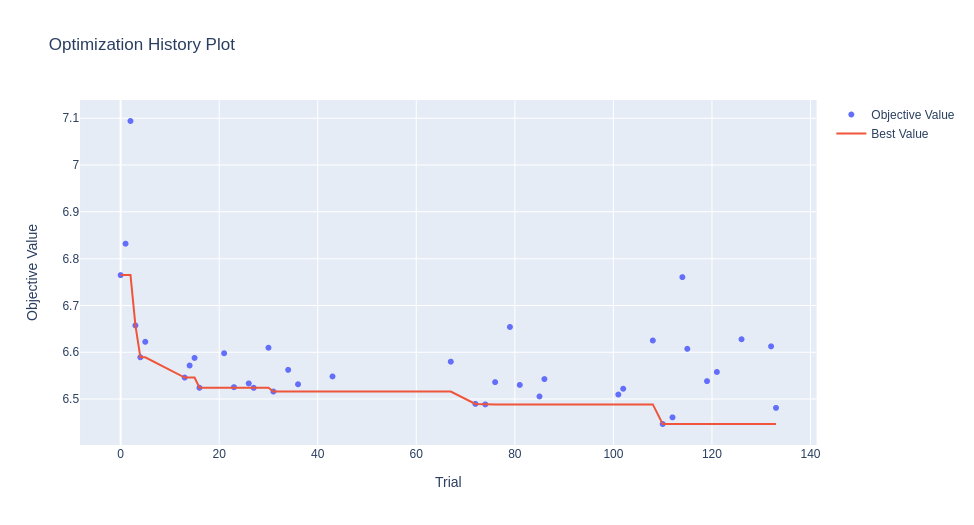
\includegraphics[scale=0.45]{opt_history.png}   }
\caption{Optimization history plot of the 136 Optuna trials.}
\label{hist}
\end{figure}


 After a warm-up period this library is capable of pruning any given run that is not achieving a satisfactory performance,  by doing this it is capable of exploring the parameter space in a more time efficient manner by only completing trial runs that have the possibility of achieving a better performance. 



There are many different samplers available in this toolbox, which essentially help us explore the parameter space by sampling different parameter values, and between all of them we chose to utilize the TPE (Tree-structured Parzen Estimator) \citep{tpe}.  
An important point of note about this sampler is that it assumes that the different hyperparameters are independent so it determines the value of a single parameter without considering any relationship between parameters. If this assumption is false the optimization  process may take more time or in some cases even miss some opportunities for further improvement when such hyperparameters have a strong relationship. We hypothesize that the hyperparameters that we chose are  independent or at the least have a weak impact on one another but since we have never tested this hypothesis it is possible that our model could be further optimized by simply picking a more robust sampler. Due to our time constraints we were unable to further explore this point.




Fig.~\ref{hist} presents the plot with the optimization history of our study and it's 196 trial runs and Fig.~\ref{optuna_all_runs} presents the loss and accuracy plots of these trials.

\begin{figure}[!ht]
\centerline{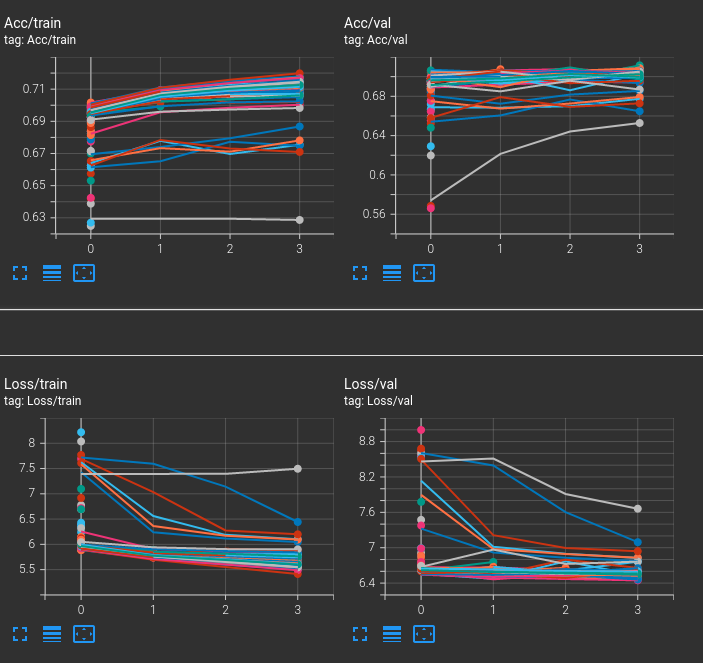
\includegraphics[scale=0.6]{figuras/optuna_all_glove_runs.png}   }
\caption{Loss and accuracy plots of the 196 Optuna trial runs.}
\label{optuna_all_runs}
\end{figure}


\begin{figure}[!ht]
\centerline{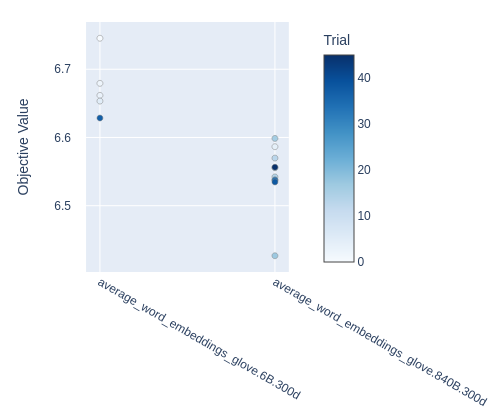
\includegraphics[scale=0.5]{slice glove editado.png}   }
 \caption{Slice plot of 43 Optuna trial runs, since the GloVe embedding trained with 840 billion parameters could achieve a better performance over it's counterpart trained with only 6 billion parameters we decided to exclude the embedding choice from the search space from our subsequent runs, as can be seen in Fig.~\ref{slice}.}
\label{sliceglove}
\end{figure}



\begin{figure}[!ht]
\centerline{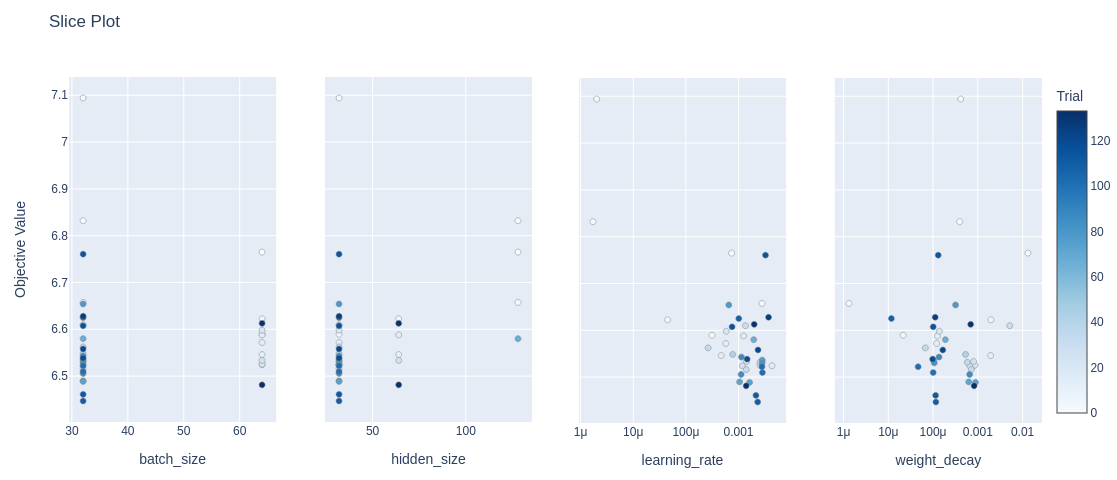
\includegraphics[scale=0.35]{slice2.png}   }
\caption{Slice plot of the optimization results found through Optuna. From the 136 trials, 95 were pruned before completion and 39 were completed. The best trial achieved a loss value of 6.446797407 with the following hyperparameter values:
    batch size= 32,
    hidden size= 32,    learning rate= 0.00231519996,
    weight decay= 0.0001155681898}
\label{slice}
\end{figure}


In Fig.~\ref{sliceglove} and Fig.~\ref{slice} we are able to see the slice plots of our parameters. Originally we were going to explore all parameters at the same time in a single study, but while we were still learning how to use Optuna it became clear that the GloVe embedding trained with 840 billion parameters could achieve a better performance over it's counterpart trained with only 6 billion parameters so we decided to exclude the embedding choice from the search space.










%!TeX root=../tese.tex
%("dica" para o editor de texto: este arquivo é parte de um documento maior)
% para saber mais: https://tex.stackexchange.com/q/78101

\chapter{Results and experiments}
\label{results}

In this chapter we will describe the experiments we performed to compare the different building blocks for our model that we described in Chapter~\ref{chap:models}. To better understand the options available to build the best model possible, we begin by analyzing the proposed embeddings, first we compare the transformer based embeddings and then add GloVe to the analysis. With the ``best'' embedding selected we compare both proposed architectures and then lastly we train our definitive model based on the results of the previous experiments.





\section{Comparing transformer based embeddings}

To compare the transformer embeddings, we trained 7 pointer networks to compute the loss and accuracy graphs for these models in the validation and training datasets. In general, after the fourth epoch of training we began to see signs of overfitting in all of our models so here we only present training results up to the fourth epoch. In Fig~\ref{7loss} we can see the L1 loss plots of training and validation. In both cases ``paraphrase-albert-small-v2''  performed significantly worse than other models at all times. The best performing model isn't as clean cut as the worst but ``distiluse-base-multilingual-cased-v1'' --- or dbmc1 as we will call it from now on --- was able to attain the lowest validation loss at the third epoch.


\begin{table}[]
\begin{tabular}{lllll}
\multicolumn{1}{l|}{Embedding}                             & Acc train & Acc val & Loss train & Loss val \\ \hline
\multicolumn{1}{l|}{distiluse-base-multilingual-cased-v1}  & 0.7296    & 0.7263  & 5.485      & 6.423    \\
\multicolumn{1}{l|}{all-mpnet-base-v2}                     & 0.7215    & 0.7172  & 5.596      & 6.407    \\
\multicolumn{1}{l|}{all-distilroberta-v1}                  & 0.724     & 0.7178  & 5.554      & 6.442    \\
\multicolumn{1}{l|}{all-MiniLM-L12-v2}                     & 0.7234    & 0.7121  & 5.549      & 6.494    \\
\multicolumn{1}{l|}{paraphrase-albert-small-v2}            & 0.709     & 0.6961  & 5.747      & 6.559    \\
\multicolumn{1}{l|}{paraphrase-multilingual-MiniLM-L12-v2} & 0.7242    & 0.7102  & 5.546      & 6.496    \\
\multicolumn{1}{l|}{paraphrase-MiniLM-L3-v2}               & 0.7245    & 0.714   & 5.51       & 6.449    \\
\multicolumn{1}{l|}{distiluse-base-multilingual-cased-v2}  & 0.7271    & 0.7144  & 5.528      & 6.437
\end{tabular}
\caption{Accuracy and Loss of the final epoch for the eight different transformer based embeddings. Amongst the eight models ``distiluse-base-multilingual-cased-v2'' achieved the lowest loss validation score at the third epoch with a loss value of 6.334 followed by dbmc1 with a loss validation of 6.374 also at the third epoch.}
\label{table:8}
\end{table}


Alongside the L1 loss we recorded the jaccard binary accuracy score of the predictions at each epoch, which can be seen in Fig.~\ref{7acc} as the train and validation accuracy.
Once again ``paraphrase-albert-small-v2'' was the worst performing model and dbmc1 was the best performing model. 


\begin{figure}[!ht]
\centerline{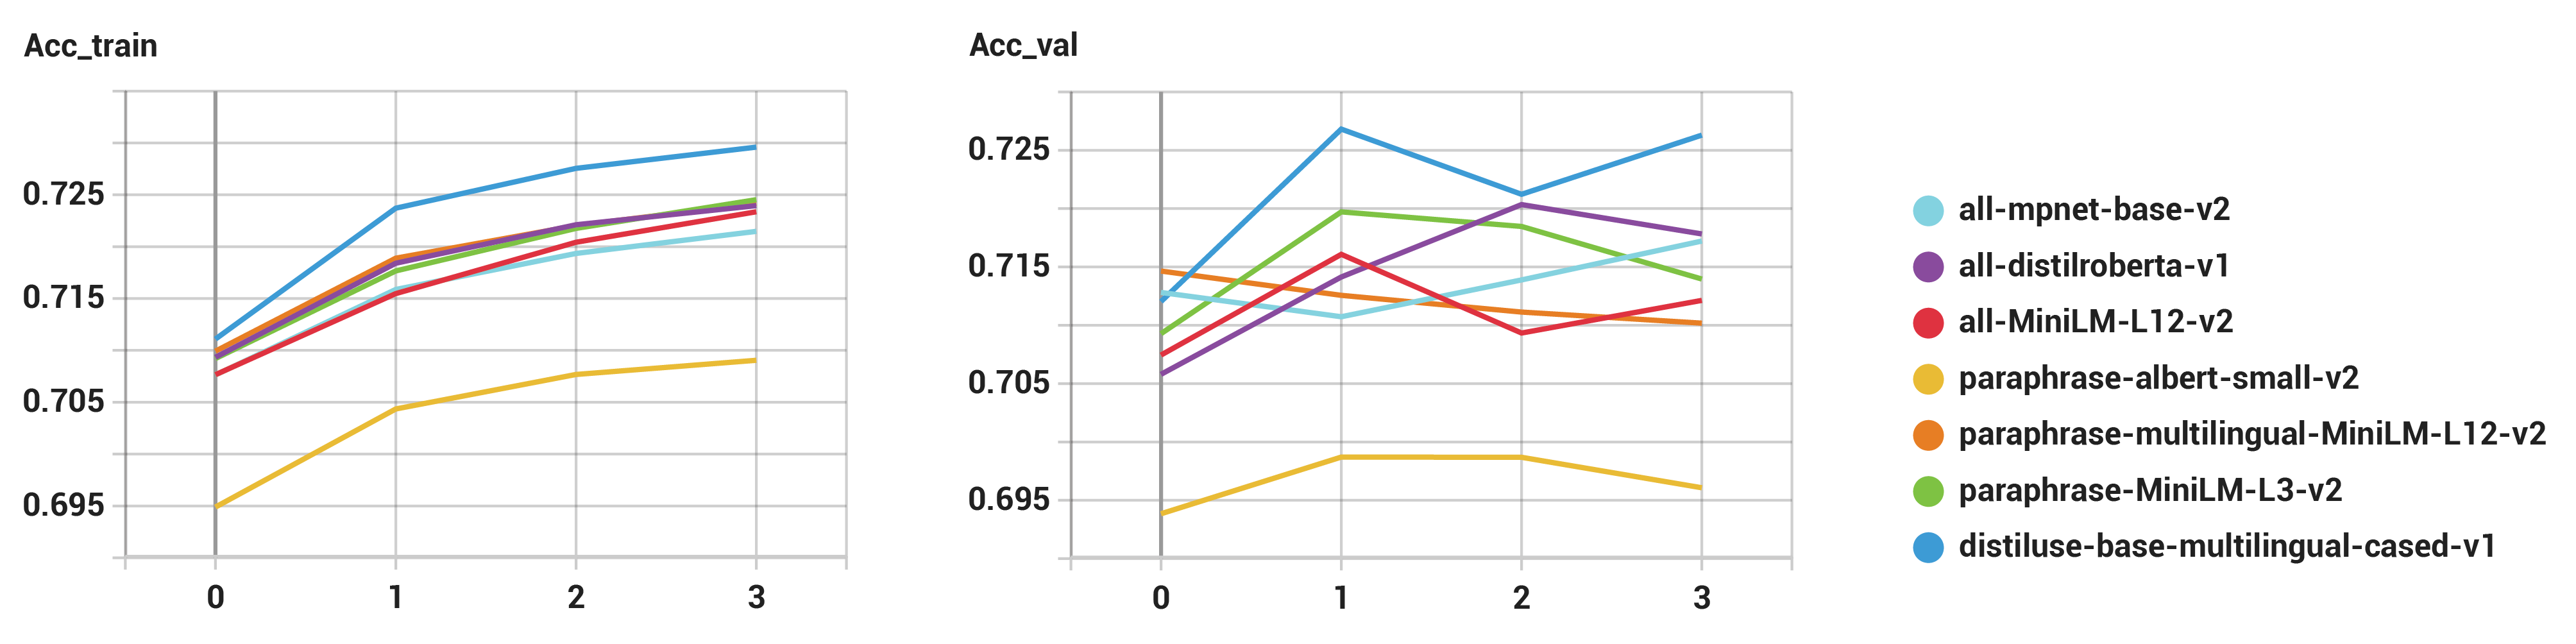
\includegraphics[width=1.1\textwidth]{figuras/7embeddings_transformer_-ACC.png}   }
\caption{Train and validation binary accuracy score of the seven transformer based models.}
\label{7acc}
\end{figure}

\begin{figure}[!ht]
\centerline{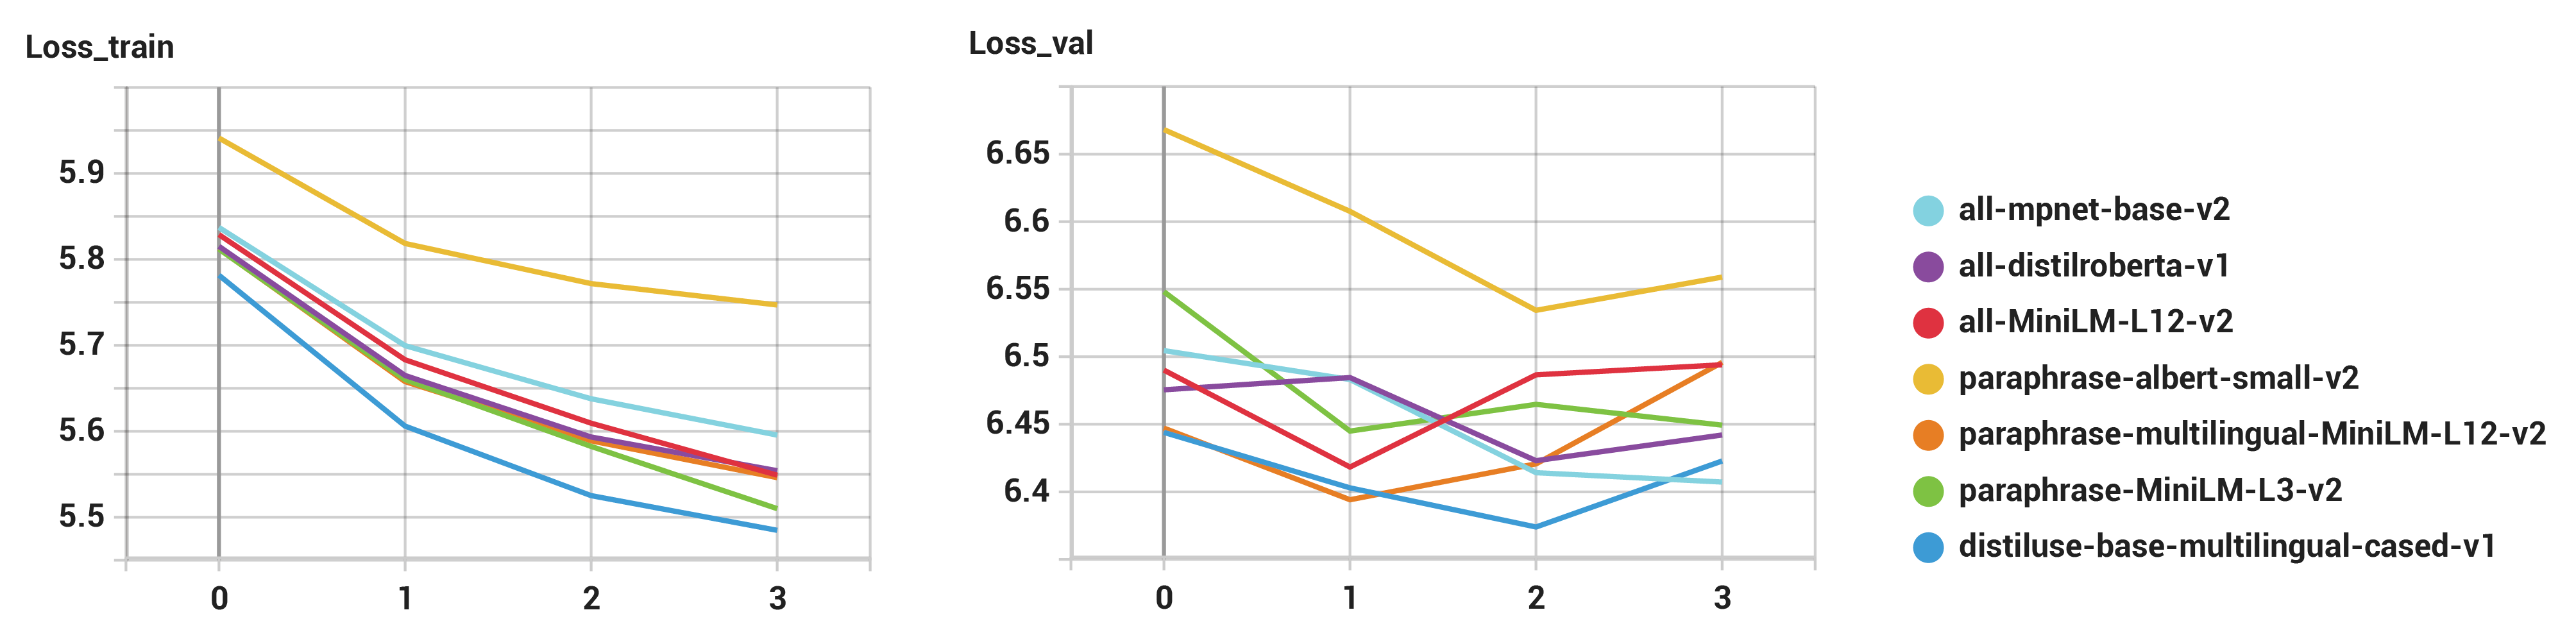
\includegraphics[width=1.1\textwidth]{figuras/7embeddings_transformer_-Loss.png}   }
\caption{L1 training and validation loss of the seven transformer based models. }
\label{7loss}
\end{figure}

Due to the unexpectedly great performance of dbmc1 we decided to test ``distiluse-base-multilingual-cased-v2'' to validate if we were correct in our initial assumption that including another 35 languages in the training process wouldn't  bring us much benefit. In Fig.~\ref{multilingual_acc} and Fig.~\ref{multilingual_loss} we can see the results of their comparison.
Against our expectations, ``distiluse-base-multilingual-cased-v2'' was capable of obtaining a lower validation  loss than its predecessor at the third epoch, however its accuracy was consistently lower in both training and validation. Since accuracy should better translate into real world performance we will be keeping dbmc1 as the best performing model overall with a validation accuracy of 72.63\%. Table~\ref{table:8} compiles the loss and accuracy results of these models.

\begin{figure}[!ht]
\centerline{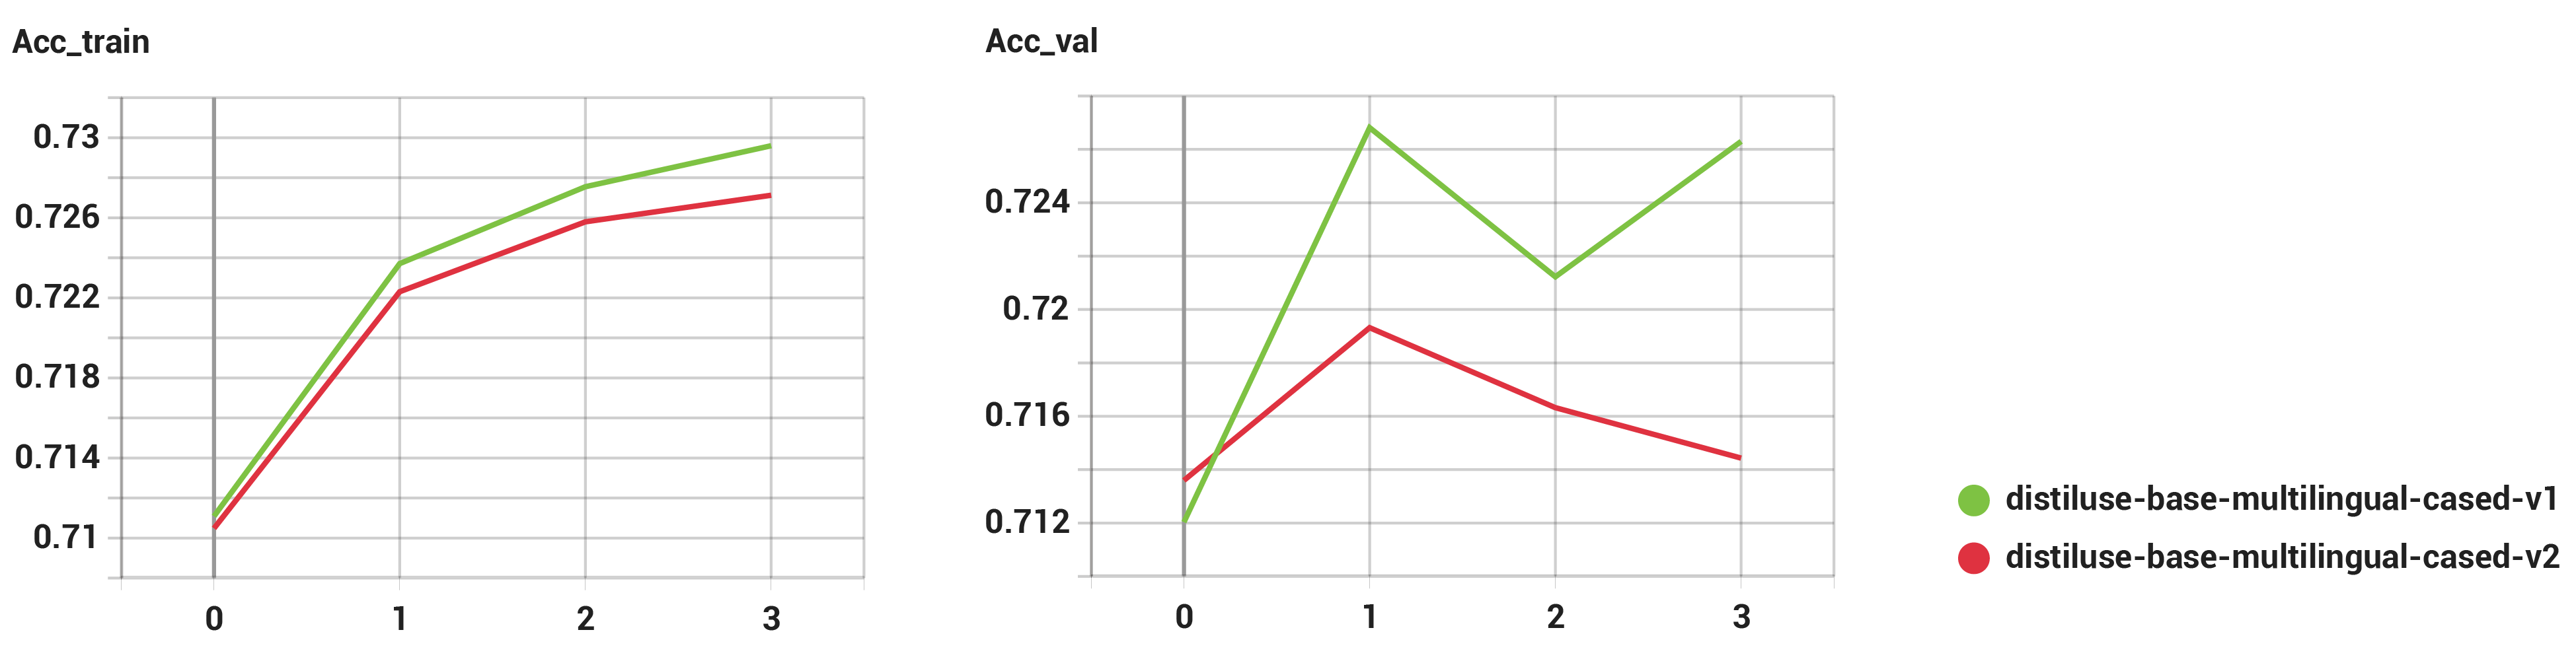
\includegraphics[width=1.1\textwidth]{figuras/multilingual_1vs2_-Acc.png}   }
\caption{Comparison of accuracy in validation and train sets between models dbmc1 and ``distiluse-base-multilingual-cased-v2''.}
\label{multilingual_acc}
\end{figure}


\begin{figure}[!ht]
\centerline{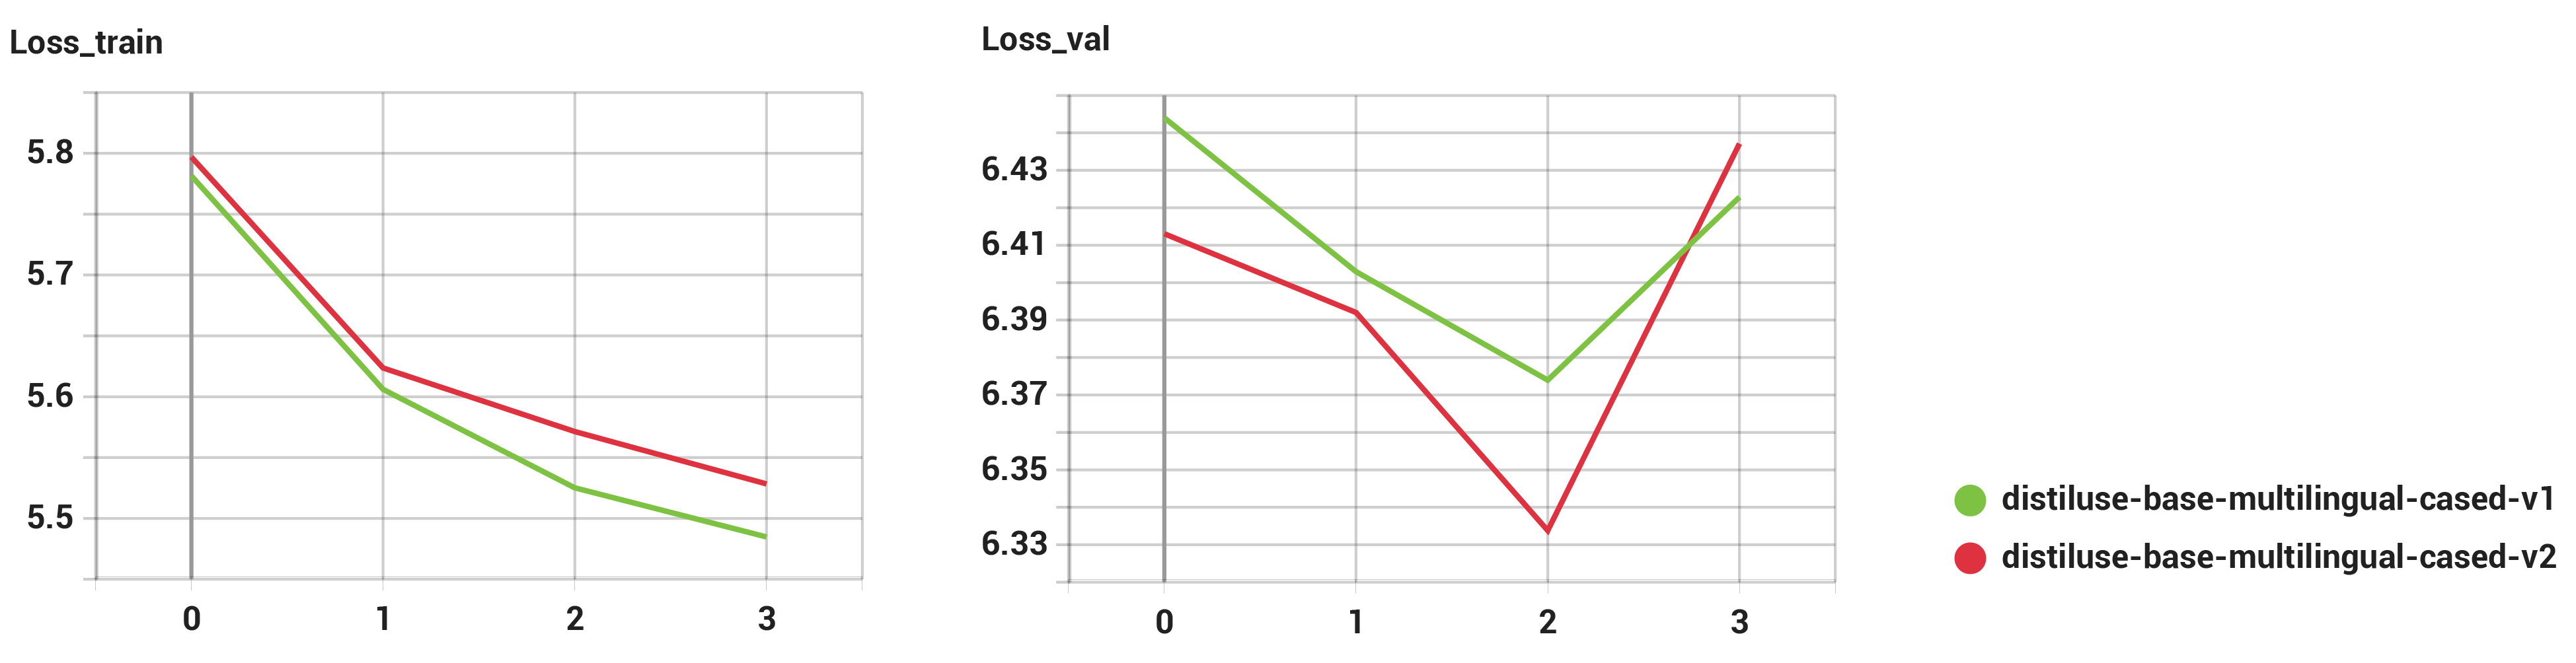
\includegraphics[width=1.1\textwidth]{figuras/multilingual_1vs2_-Loss.png}   }
\caption{Comparison of loss in validation and train sets between models dbmc1 and ``distiluse-base-multilingual-cased-v2''.}
\label{multilingual_loss}
\end{figure}

\newpage

\section{Adding GloVe to the comparison}


In Fig.~\ref{glove_loss} and Fig.~\ref{glove_acc} we compare the pointer network models trained with transformer based embeddings with their GloVe counterpart, which was the best performing model we obtained through Optuna in section \ref{optuna}. In the interest of clarity we decided to omit some of the  transformer models from the graphs to avoid clutter, we plot only the best performing transformer-based model and the two other that are adjacent in performance to the GloVe-based model. The graph makes it clear that the GloVe-based model performed consistently worse than all the transformer-based models, except for model ``paraphrase-albert-small-v2'' which was the worst performing one. Table~\ref{table:glove} compiles the final accuracy and loss of all of the presented transformer models and the GloVe model.

% Please add the following required packages to your document preamble:
% \usepackage[table,xcdraw]{xcolor}
% If you use beamer only pass "xcolor=table" option, i.e. \documentclass[xcolor=table]{beamer}
\begin{table}[]
\begin{tabular}{l|llll}
Embedding                             & Acc train & Acc val & Loss train & Loss val \\ \hline
distiluse-base-multilingual-cased-v1  & 0.7296    & 0.7263  & 5.485      & 6.423    \\
all-mpnet-base-v2                     & 0.7215    & 0.7172  & 5.596      & 6.407    \\
all-distilroberta-v1                  & 0.724     & 0.7178  & 5.554      & 6.442    \\
all-MiniLM-L12-v2                     & 0.7234    & 0.7121  & 5.549      & 6.494    \\
paraphrase-albert-small-v2            & 0.709     & 0.6961  & 5.747      & 6.559    \\
paraphrase-multilingual-MiniLM-L12-v2 & 0.7242    & 0.7102  & 5.546      & 6.496    \\
paraphrase-MiniLM-L3-v2               & 0.7245    & 0.714   & 5.51       & 6.449    \\
distiluse-base-multilingual-cased-v2  & 0.7271    & 0.7144  & 5.528      & 6.437    \\
\rowcolor[HTML]{F9F5E9} 
glove.840B.300d                         & 0.7123    & 0.7046  & 5.64       & 6.447   
\end{tabular}
\caption{Accuracy and Loss of the final epoch for the eight different transformer based embeddings and the GloVe based embedding.}
\label{table:glove}
\end{table}


\begin{figure}[!ht]
\centerline{\includegraphics[width=1.1\textwidth]{figuras/glove_vs_transformer_-ACC.png}   }
\caption{Plots comparing the training and validation accuracy of four pointer networks trained with a GloVe embedding and 3 other transformer based embedding.}
\label{glove_acc}
\end{figure}

\begin{figure}[!ht]
\centerline{\includegraphics[width=1.1\textwidth]{figuras/glove_vs_transformer_-Loss.png}} 
\caption{Plots comparing the training and validation loss of four pointer networks trained with a GloVe embedding and 3 other transformer based embedding.}
\label{glove_loss}
\end{figure}


\newpage

\section{Comparing architectures}

 
In Fig.~\ref{arq_acc} and Fig.~\ref{arq_loss} we compare our two architectures, the pointer network and our so-called ``simple RNN''. We trained both models with the best performing embedding we found in previous sections, the dbmc1 embedding, and found that the Ptr-Net outperformed the simple RNN in all 4 metrics as can be seen in Table~\ref{table:arq}. 


\begin{figure}[!ht]
\centerline{\includegraphics[width=1.1\textwidth]{figuras/arquiteturas_-ACC.png}   }
\caption{Plots comparing the training and validation accuracy of our two architectures trained with the  dbmc1 embedding.}
\label{arq_acc}
\end{figure}

\begin{figure}[!ht]
\centerline{\includegraphics[width=1.1\textwidth]{figuras/arquiteturas_-Loss.png}   }
\caption{Plots comparing the training and validation loss of our two architectures trained with the dbmc1 embedding.}
\label{arq_loss}
\end{figure}

\begin{table}[]
\begin{tabular}{l|llll}
Architecture & Acc train & Acc val & Loss train & Loss val \\ \hline
Ptr-Net      & 0.7296    & 0.7263  & 5.485      & 6.423    \\
Simple RNN   & 0.7105    & 0.7115  & 5.827      & 6.589   
\end{tabular}
\caption{Table of the final (fourth epoch) loss and accuracy in the training and validation sets for our two different architectures.}
\label{table:arq}
\end{table}

\section{Best Model}

Taking into account all our previous findings we can conclude that the pointer network architecture combined, with the dbmc1 embedding and the hyperparameters found by Optuna form our best performing model, Fig.~\ref{fig:final_model} illustrates succinctly this final model.  In Fig.~\ref{best_acc} and Fig.~\ref{best_loss} we present the accuracy and loss plots for this model in the training and testing datasets and in Table~\ref{table:best} we compile its final accuracy and loss scores.


\begin{figure}[!ht]
\centerline{\includegraphics[width=0.8\textwidth]{figuras/final_model.png}   }
\caption{Illustration of our final and best performing model. As previously mentioned, the hyper-parameters were chosen based on our Optuna experiments.}
\label{fig:final_model}
\end{figure}

\begin{table}[]
\begin{tabular}{l|llll}
Architecture                                                                                                & Acc train & Acc test & Loss train & Loss test \\ \hline
\begin{tabular}[c]{@{}l@{}}Ptr-Net and distiluse-base-\\ multilingual-cased-v1 \\ (Best Model)\end{tabular} & 0.7274    & 0.7275   & 5.529      & 5.768    
\end{tabular}
\caption{Accuracy and loss of the final epoch in the training and test sets for the final model, trained with the Ptr-Net architecture and the dbmc1 embedding.}
\label{table:best}
\end{table}

\begin{figure}[!ht]
\centerline{\includegraphics[width=1.1\textwidth]{figuras/best_model_-ACC.png}   }
\caption{Training and testing plots of accuracy of our best performing model in validation. Final accuracy value: 0.7275.}
\label{best_acc}
\end{figure}

\begin{figure}[!ht]
\centerline{\includegraphics[width=0.8\textwidth]{figuras/best_model_-Loss.png}   }
\caption{Training and testing plots of loss of our best performing model in validation. Final loss value: 5.768.}
\label{best_loss}
\end{figure}


As an alternative, dbmc1 could be swapped by the GloVe embedding in the interest of speeding up inference time. Albeit when doing a single prediction the inference time of dbmc1 is greater than that of GloVe it is not as significant of an increase as when training the models where the process takes multiple days for each transformer based embedding over the few hours of GloVe based models. This decision should be taken case by case, for some applications keeping the inference time as small as possible may be more important than the 0.01\% performance gain of using dbmc1.



Whatever choice is made in a hypothetical deployment aside, we believe this model achieved the objectives we set. In conjunction with a language server it can easily execute function extraction refactorings and in conjunction with a refactoring opportunity detector these 3 components together could become a IDE plugin that automates the entirety of the function extraction process.

\subsection{Publication of results}

The student is preparing to submit these results as a scientific paper to a peer reviewed journal.



%!TeX root=../tese.tex
%("dica" para o editor de texto: este arquivo é parte de um documento maior)
% para saber mais: https://tex.stackexchange.com/q/78101

\chapter{Conclusion}



In conclusion we believe we were able to achieve both of the goals set at the beginning of this project, our results show that is indeed possible for a deep learning model to predict fine-grained refactorings and we were successful in creating a number of models for automated function extraction refactoring. 

Our final model consisted of the pointer network architecture the ``distiluse-base-multilingual-cased-v1'' embedding  and the hyperparameter values obtained with Optuna,  with this model we achieved a test loss and a test accuracy of  5.768 and 0.7275 respectively. We believe this results once again corroborate the hypothesis of naturality and show the soundness of our approach.

However, the models we trained were always hovering an accuracy of around 70\%. Changing architectures, embeddings and hyperparameter values had a clear effect in the performance of the models but always in an incremental fashion with small gains to performance.

We hypothesize that to achieve significant gains in performance we would need to explore embeddings that also leverage the source code itself (by, for example, utilizing abstract syntax trees) instead of solely relying on natural language models. This is a hypothesis that we are interested in pursuing in future work.


We were also able to develop a new Java code refactoring dataset for function extractions that was over 60\% bigger than the biggest dataset of its type published at the moment of elaboration of this report.


Through this we also hope to show that deep learning models are capable of predicting fine-grained refactorings, that they are able to dictate how exactly a snippet of code should be altered to obtain a successful refactoring.



% \par   %(???? ta na quali mas n no novo template, acho.)
%%%%%%%%%%%%%%%%%%%%%%%%%%%% APÊNDICES E ANEXOS %%%%%%%%%%%%%%%%%%%%%%%%%%%%%%%%

% Um apêndice é algum conteúdo adicional de sua autoria que faz parte e
% colabora com a ideia geral do texto mas que, por alguma razão, não precisa
% fazer parte da sequência do discurso; por exemplo, a demonstração de um
% teorema intermediário, as perguntas usadas em uma pesquisa qualitativa etc.
%
% Um anexo é um documento que não faz parte da tese (em geral, nem é de sua
% autoria) mas é relevante para o conteúdo; por exemplo, a especificação do
% padrão técnico ou a legislação que o trabalho discute, um artigo de jornal
% apresentando a percepção do público sobre o tema da tese etc.
%
% Os comandos appendix e annex reiniciam a numeração de capítulos e passam
% a numerá-los com letras. "annex" não faz parte de nenhuma classe padrão,
% foi criado para este modelo. Se o trabalho não tiver apêndices ou anexos,
% remova estas linhas.
%
% Diferentemente de \mainmatter, \backmatter etc., \appendix e \annex não
% forçam o início de uma nova página. Em geral isso não é importante, pois
% o comando seguinte costuma ser "\chapter", mas pode causar problemas com
% a formatação dos cabeçalhos. Assim, vamos forçar uma nova página antes
% de cada um deles.

%%%% Apêndices %%%%

\makeatletter
\if@openright\cleardoublepage\else\clearpage\fi
\makeatother

\pagestyle{appendix}

\appendix

% \addappheadtotoc acrescenta a palavra "Apêndice" ao sumário; se
% só há apêndices, sem anexos, provavelmente não é necessário.
\addappheadtotoc

%!TeX root=../tese.tex
%("dica" para o editor de texto: este arquivo é parte de um documento maior)
% para saber mais: https://tex.stackexchange.com/q/78101

\chapter{AST Printer}
\label{an:astcoisas}


The code utilized to print the AST present in Fig.~\ref{fig:ast} can be seen in Listing~\ref{listing:printer}.


\begin{listing}[!ht]
\inputminted[linenos, ]{java}{conteudo/code/ast_printer.java}
\caption{Code utilized to print Java ASTs using the \texttt{JavaParser} package.}
\label{listing:printer}
\end{listing}


\chapter{Data Scrapping Source Code}
\label{an:code_data}


In the interest of reproducibility and a higher scientific standard, we provide the source code utilized to generate the dataset described in this work and most of its results.

\begin{listing}[!ht]
\inputminted[linenos, breaklines]{bash}{conteudo/code/clona_tudo.sh}
\caption{Small bash script used to clone all the repositories listed in 'repos.txt'.}
\label{listing:clona}
\end{listing}




\begin{listing}[!ht]
\inputminted[linenos, breaklines]{bash}{conteudo/code/mina_tudo.sh}
\caption{Small bash script used to parallelize the mining of refactorings in all the repositories previously cloned.}
\label{listing:mina}
\end{listing}

\newpage


\begin{code}
\inputminted[linenos, breaklines]{python}{conteudo/code/create_db.py}
\caption{Python script used to process the JSON files into an actionable SQLite database of function extraction refactorings and their metadata.}
\label{listing:db}
\end{code}



\chapter{$\beta$ impact on \textit{softargmax}}
\label{ap:beta}


Normally this discussion would be a part of the main thesis, however we feel that it lacks in rigor to convince skeptic readers but simply discarding it would be omission on our part. We wished to replicate this experiment in a matter to have statistical significance to demonstrate our findings but due to time constraints and the somewhat out-of-scope aspect of this experiment, training thousands of models for this was not feasible. So here we present a simple snapshot of what trying to overfit a model over a reduced dataset while varying the value of $\beta$ would look like, Fig.~\ref{beta_loss} presents the training loss plot.

While we were performing this experiment we realized that there was too much variability between runs with a same $\beta$ value to be able to precisely describe its impact. However, some behaviors were found to be consistent: no model with a $\beta$ value of $1000$ or above was able to overfit the data, i.e. they were incapable of learning with an essentially fixed loss across epochs. Higher values of $\beta$ lead to a better approximation of the argmax function but when $\beta$ is to big it also starts approximating its discontinuity leading to a broken gradient flow and making the model ability to learn to come to a halt. To better understand this phenomenon and $\beta$ impact on learning more experiments to analyze the spread of the loss function would be necessary.



\begin{figure}[!ht]
\centerline{\includegraphics[width=0.9\textwidth]{figuras/betas_-Loss.png}   }
\caption{Training loss plot over the training epochs of a pointer network model for varying $\beta$ values. Training was done over only 10 data points in order o explore the ability of the model to overfit, the initial rational was that if a model cannot even overfit a minuscule dataset it is not suitable for training with the entire dataset or that it may even be be broken.}
\label{beta_loss}
\end{figure}
\par

%%%% Anexos %%%%

% \makeatletter
% \if@openright\cleardoublepage\else\clearpage\fi
% \makeatother

% \pagestyle{appendix} % repete o anterior, caso você não use apêndices

% \annex

% % \addappheadtotoc acrescenta a palavra "Anexo" ao sumário; se
% % só há anexos, sem apêndices, provavelmente não é necessário.
% \addappheadtotoc

% %!TeX root=../tese.tex
%("dica" para o editor de texto: este arquivo é parte de um documento maior)
% para saber mais: https://tex.stackexchange.com/q/78101

% \par


%%%%%%%%%%%%%%% SEÇÕES FINAIS (BIBLIOGRAFIA E ÍNDICE REMISSIVO) %%%%%%%%%%%%%%%%

% O comando backmatter desabilita a numeração de capítulos.
\backmatter

\pagestyle{backmatter}

% Espaço adicional no sumário antes das referências / índice remissivo
\addtocontents{toc}{\vspace{2\baselineskip plus .5\baselineskip minus .5\baselineskip}}

% A bibliografia é obrigatória

\printbibliography[
  title=\refname\label{bibliografia}, % "Referências", recomendado pela ABNT
  %title=\bibname\label{bibliografia}, % "Bibliografia"
  heading=bibintoc, % Inclui a bibliografia no sumário
]

% \printindex % imprime o índice remissivo no documento (opcional)

\end{document}
